%! TEX program = xelatex
% 
% Versi 1.1
%
% Template Tugas Akhir 
% Program Studi Sistem dan Teknologi Informasi
% Sekolah Teknik Elektro dan Informatika
% Institut Teknologi Bandung
% 
% Dibuat oleh: IGB Baskara Nugraha 
% Email: baskara@itb.ac.id 
% 
%
% Petunjuk penggunaan:
% 1. Ada 2 file utama, yaitu TA.tex (file ini) dan daftar-pustaka.bib (file daftar pustaka).
% 2. Sunting TA.tex sesuai dengan kebutuhan Anda.
% 3. Sunting atau generate isi daftar-pustaka.bib dengan referensi yang Anda gunakan, sesuai dengan format BibLaTeX.
% 4. Simpan kedua file tersebut dalam satu folder yang sama.
% 5. Kompilasi file TA.tex menggunakan XeLaTeX dan Biber (lihat urutan cara kompilasi di bawah).
% 6. Hasil kompilasi adalah file TA.pdf yang siap dicetak.
% 
% Urutan cara kompilasi (melalui command line):
% 1. xelatex TA.tex
% 2. biber TA      
% 3. xelatex  TA.tex
% 4. xelatex  TA.tex
%
% Catatan:
% - Pastikan Anda telah menginstal paket-paket LaTeX yang diperlukan, termasuk
%   biblatex-chicago dan fontspec.
% - Gunakan editor LaTeX yang mendukung XeLaTeX, seperti TeXstudio, Overleaf, atau lainnya.
% - Jika meenggunakan Visual Studio Code sebagai editor, pastikan mengatur "latex-workshop.latex.tools" dan
%   "latex-workshop.latex.recipes" untuk mendukung XeLaTeX dan Biber dengan cara menambahkan konfigurasi berikut:
%   "latex-workshop.latex.tools": [ 
%       {
%           "name": "xelatex",
%           "command": "xelatex",
%           "args": [
%               "-synctex=1",
%               "-interaction=nonstopmode",
%               "-file-line-error",
%               "%DOC%"
%           ]
%       },
%       {
%           "name": "biber",
%           "command": "biber",
%           "args": [
%               "%DOCFILE%"
%           ]
%       }
%   ],
%   "latex-workshop.latex.recipes": [
%       {
%           "name": "xelatex -> biber -> xelatex*2",
%           "tools": [
%               "xelatex",
%               "biber",
%               "xelatex",
%               "xelatex"
%           ]
%       }
%   ]
% - Untuk referensi lebih lanjut tentang penggunaan BibLaTeX dengan gaya Chicago, silakan merujuk ke dokumentasi resmi BibLaTeX.
%   https://ctan.org/pkg/biblatex-chicago
% - Untuk referensi lebih lanjut tentang penggunaan XeLaTeX dan fontspec, silakan merujuk ke dokumentasi resmi fontspec.
%   https://ctan.org/pkg/fontspec
% - Selamat menyusun dokumen tugas akhir Anda!
%
\documentclass[12pt,a4paper]{book}

% --- Main packages ---
\usepackage[utf8]{inputenc} % for UTF-8 encoding
\usepackage{fontspec} % for font selection
\usepackage[indonesian]{babel} % untuk bahasa Indonesia
\usepackage{csquotes} % for context-sensitive quotation facilities
\usepackage{setspace} % for line spacing
\usepackage{graphicx} % for images
\usepackage{caption} % for customizing captions
\usepackage{subcaption} % for sub-figures

\usepackage{tocloft} % for customizing table of contents
\usepackage{titlesec} % for customizing titles
\usepackage{lipsum} % for dummy text (lorem ipsum text)
\usepackage{floatrow} % for customizing float (figure and table) positions
\usepackage{listings} % for code listing
\usepackage{amsmath} % for math
\usepackage{amssymb} % for math symbols
\usepackage[shortlabels]{enumitem} % for customizing lists
\usepackage[skip=12pt]{parskip} % for spacing between paragraphs
\usepackage{longtable} % for long tables
\usepackage{booktabs} % for better table rules
\usepackage[bahasai]{datetime2} % for date formatting in Indonesian
\usepackage{geometry} % for page margins
\usepackage{algorithm} % for algorithms
\usepackage{algorithmicx} % for algorithmic environment
\usepackage{algpseudocode} % for pseudocode
\usepackage{microtype} % Untuk optimasi typography dan spacing
\usepackage{floatrow} % for customizing float (figure and table) positions
\usepackage{array} % for better arrays (eg. in tabular environment)
\usepackage{threeparttable} % for tables with notes
\usepackage{tabularx} % for tables with adjustable-width columns
\usepackage{xcolor} % for color definitions
\usepackage[title,titletoc]{appendix} % for appendix management
\usepackage{csquotes} % for context-sensitive quotation facilities
\usepackage[hidelinks]{hyperref} % for hyperlinks


\setmainfont{Times New Roman} % set main font to Times New Roman
\onehalfspacing % spasi 1.5

% --- Bibliography menggunakan BibLaTeX dengan gaya Chicago ---
\usepackage[
    backend=biber,
    authordate,
    language=english,
    autolang=other
]{biblatex-chicago}
\addbibresource{daftar-pustaka.bib}

% --- Terjemahan istilah daftar pustaka ke Bahasa Indonesia ---
\DefineBibliographyStrings{english}{
  and          = {dan},
  andothers    = {dkk.},
  editor       = {penyunting},
  editors      = {penyunting},
  translator   = {penerjemah},
  byeditor     = {disunting oleh},
  bytranslator = {diterjemahkan oleh},
  in           = {dalam},
  edition      = {edisi},
  pages        = {hal.},
  page         = {hal.},
  volume       = {vol.},
  number       = {no.},
  urlseen      = {diakses pada},
  url          = {tautan},
}

% --- ubah format sitasi menjadi (Author Year) ---
\let\oldcite\cite
\renewcommand{\cite}{\parencite}

% --- hilangkan koma sebelum 'dan' pada daftar pustaka ---
\renewcommand*{\finalandcomma}{} 

% --- hyperlinks setup ---
\hypersetup{
    colorlinks=true,
    linkcolor=black,
    citecolor=black,
    urlcolor=black
}

% -- No Header dan No Footer ---
\pagestyle{plain}

% --- Ubah nama list of listing ke "DAFTAR LISTING" ---
\renewcommand{\lstlistlistingname}{DAFTAR \textit{LISTING}} 
\renewcommand{\lstlistingname}{\textit{Listing}}
\lstset{basicstyle=\ttfamily\footnotesize,breaklines=true}

% --- Ubah nama list of algorithm ke "DAFTAR ALGORITMA" ---
\renewcommand{\algorithmname}{Algoritma}
\renewcommand{\listalgorithmname}{DAFTAR ALGORITMA}
\lstset{basicstyle=\ttfamily\footnotesize,breaklines=true}
\renewcommand{\thealgorithm}{\thechapter.\arabic{algorithm}}

% Create list of equations
\newlistof{myequations}{equ}{DAFTAR PERSAMAAN}
\setlength{\cftmyequationsnumwidth}{3em}
\renewcommand{\cftmyequationsaftersnum}{\hspace{0.5em}}

% Equation caption command (must be used inside numbered line)
\newcommand{\eqcaption}[1]{%
  \addcontentsline{equ}{myequations}
  {\protect\numberline{\theequation}#1}
}
\makeatletter
\renewcommand{\listofmyequations}{%
  \chapter*{\centering\large\bfseries DAFTAR PERSAMAAN}
  \@starttoc{equ}
}
\makeatother

\renewcommand \cftchapdotsep{4.5} % Atur jarak titik-titik pada daftar isi

%\cftsetrmarg{4em}  % agar judul subbab tidak mepet ke nomor halaman di daftar isi (optional)
% -- Atur indentasi judul bab, subbab, dan subsubbab di daftar isi ---
\setlength{\cftchapindent}{0em}
\setlength{\cftchapnumwidth}{1.8em}
\setlength{\cftsecindent}{1.8em}
\setlength{\cftsecnumwidth}{2.4em}
\setlength{\cftsubsecindent}{4.2em}
\setlength{\cftsubsecnumwidth}{2.8em}
\setlength{\cftsubsubsecindent}{7.0em}
\setlength{\cftsubsubsecnumwidth}{3.2em}

% --- Ubah nama bulan ke Bahasa Indonesia ---
\renewcommand*{\DTMbahasaimonthname}[1]{%
  \ifcase#1 %
    \or Januari%  % 1st month
    \or Februari%  % 2nd month
    \or Maret%  % 3rd month
    \or April%  % 4th month
    \or Mei%  % 5th month
    \or Juni%  % 6th month
    \or Juli%  % 7th month
    \or Agustus%  % 8th month
    \or September%  % 9th month
    \or Oktober%  % 10th month
    \or November%  % 11th month
    \or Desember%  % 12th month
  \fi
}

% --- Atur margin halaman untuk single-sided format (satu muka) ---
\geometry{
      a4paper,
      inner=4cm,
      outer=3cm,
      top=3cm,
      bottom=3cm
}

% --- LISTINGS STYLE FOR PYTHON CODE ---
% --- Silakan diubah sesuai selera dan kebutuhan ---
% Define colors for syntax highlighting
\definecolor{codegreen}{rgb}{0,0.6,0}
\definecolor{codegray}{rgb}{0.5,0.5,0.5}
\definecolor{codepurple}{rgb}{0.58,0,0.82}
\definecolor{backcolour}{rgb}{0.95,0.95,0.92}

% Configure listings style
\lstdefinestyle{pythonstyle}{
    backgroundcolor=\color{backcolour},   
    commentstyle=\color{codegreen},
    keywordstyle=\color{magenta},
    numberstyle=\tiny\color{codegray},
    stringstyle=\color{codepurple},
    basicstyle=\ttfamily\footnotesize,
    breakatwhitespace=false,         
    breaklines=true,                 
    captionpos=b,                    
    keepspaces=true,                 
    numbers=left,                    
    numbersep=5pt,                  
    showspaces=false,                
    showstringspaces=false,
    showtabs=false,                  
    tabsize=4,
    language=Python
}
\lstset{style=pythonstyle}
% --- END OF LISTINGS STYLE FOR PYTHON CODE ---

% --- LISTINGS STYLE FOR JAVASCRIPT CODE ---
\lstdefinestyle{jsstyle}{
    backgroundcolor=\color{backcolour},
    commentstyle=\color{codegreen},
    keywordstyle=\color{magenta},
    numberstyle=\tiny\color{codegray},
    stringstyle=\color{codepurple},
    basicstyle=\ttfamily\footnotesize,
    breakatwhitespace=false,
    breaklines=true,
    captionpos=b,
    keepspaces=true,
    numbers=left,
    numbersep=5pt,
    showspaces=false,
    showstringspaces=false,
    showtabs=false,
    tabsize=2,
    language=Java,
    morekeywords={const,let,async,await,function,class,require,module,exports,
                  try,catch,finally,this,new,typeof,for,of,if,else,return}
}
% --- END OF LISTINGS STYLE FOR JAVASCRIPT CODE ---

% --- FORMAT TAMPILAN JUDUL BAB, SUBBAB, JUDUL GAMBAR DAN TABEL ---
\setcounter{tocdepth}{4} % kedalaman daftar isi sampai subsubbab
\setcounter{secnumdepth}{4} % kedalaman penomoran sampai subsubbab
% --- Judul Bab ---
\titleformat{\chapter}[display]
      {\centering\normalfont\large\bfseries} % Commands for the entire chapter title
      {\MakeUppercase \chaptertitlename\ \thechapter}{0pt}{\large} % Chapter number format
      \renewcommand\thechapter{\Roman{chapter}}
% --- Atur spasi sebelum dan sesudah judul bab/chapter ---  
\titlespacing{\chapter}{0pt}{0pt}{5pt}
\titlespacing{\section}{0pt}{6pt}{6pt}
\titlespacing{\subsection}{0pt}{6pt}{6pt}
\titlespacing{\subsubsection}{0pt}{6pt}{6pt}

% --- Judul Subbab dan Subsubbab ---
\titleformat{\section}
	{\normalfont\bfseries}
	{\thesection}{1em}{}
\titleformat{\subsection}
	{\normalfont\bfseries}
	{\thesubsection}{1em}{}
\titleformat{\subsubsection}
	{\normalfont\bfseries}
	{\thesubsubsection}{1em}{}

% --- Gambar ---
\captionsetup[figure]{
  labelsep=space, 
  format=hang
}  
\floatsetup[figure]{
  capposition=bottom
} 
% --- Tabel ---
\captionsetup[table]{
  labelsep=space, 
  format=hang
} 
\floatsetup[table]{
  capposition=top, 
  objectset=centering, 
  captionskip=6pt
} 
% --- Listing ---
\captionsetup[lstlisting]{
  labelsep=space, 
  format=hang, 
  justification=raggedright, 
  singlelinecheck=false
}
\floatsetup[lstlisting]{
  capposition=top
}
% --- Algoritma ---
\captionsetup[algorithm]{
  labelsep=space, 
  format=hang, 
  justification=raggedright, 
  singlelinecheck=false
}
\floatsetup[algorithm]{
  capposition=top
}

% --- Atur indentasi paragraf ---
\setlength{\parindent}{0pt}
\setlength{\parskip}{12pt plus 2pt minus 1pt}

\setlist[enumerate]{nosep, topsep=-10pt} % mengurangi spasi antar item dan atas bawah daftar
\setlist[itemize]{nosep, topsep=-10pt} % mengurangi spasi antar item dan atas bawah daftar
\usepackage{multirow}
\usepackage[table]{xcolor} % Required for \cellcolor
\usepackage{float}         % Required for the [H] placement

% ==========================================
% AWAL DOKUMEN
% ==========================================
\begin{document}

% ==========================================
% HALAMAN AWAL (FRONTMATTER)
% ==========================================
\frontmatter
% --- Atur format daftar isi untuk bagian frontmatter ---
\addtocontents{toc}{\protect\setlength{\cftbeforechapskip}{0pt}}
\addtocontents{toc}{\protect\renewcommand{\protect\cftchapfont}{\protect\normalfont}}
\addtocontents{toc}{\protect\renewcommand{\protect\cftchappagefont}{\protect\normalfont}}
\renewcommand{\cftchapleader}{\cftdotfill{\cftchapdotsep}}


% ==========================================

\begin{titlepage}
\begin{center}

    
    \vspace*{2cm}
    
    {\Large\bfseries\uppercase{PERANCANGAN SISTEM \textit{BUSINESS INTELLIGENCE} BERBASIS \textit{RULE-BASED CHATBOT} DENGAN \textit{TIME SERIES FORECASTING} DAN TEKNOLOGI BAHASA ALAMI UNTUK ANALISIS DAN PREDIKSI KINERJA BISNIS} 
}\\
     \vspace{2cm}

    {\Large \textbf{Laporan Tugas Akhir}}\\


    \vspace{2cm}
    
    
    {\large Oleh}\\[0.3cm]
    \textbf{
    {\large Thalita Zahra Sutejo}\\
    {\large 18222023}
    }\\

    \vspace{2cm}
    
    \begin{figure}[h]
    \centering
    
\includegraphics[width=0.2\textwidth]{images/ganesha.jpg}
    \end{figure}
    
    
    % \vspace{1cm}
    \vfill

    \textbf{
    {\large PROGRAM STUDI SISTEM DAN TEKNOLOGI INFORMASI}\\
    {\large SEKOLAH TEKNIK ELEKTRO DAN INFORMATIKA}\\
    {\large INSTITUT TEKNOLOGI BANDUNG}\\
    {\large \DTMlangsetup{showdayofmonth=false,showmonthname=true,showyear=true}\today}
    }
\end{center}
\end{titlepage}
\chapter*{LEMBAR PENGESAHAN}
\addcontentsline{toc}{chapter}{LEMBAR PENGESAHAN}


\begin{center}
    \vspace{2cm}
  {\large\bfseries PERANCANGAN SISTEM \textit{BUSINESS INTELLIGENCE} BERBASIS \textit{RULE-BASED CHATBOT} DENGAN \textit{TIME SERIES FORECASTING} DAN TEKNOLOGI BAHASA ALAMI UNTUK ANALISIS DAN PREDIKSI KINERJA BISNIS}\\
     \vspace{2cm}

  {\Large \textbf{Laporan Tugas Akhir}}\\


  \vspace{1.5cm}


  {\large Oleh}\\[0.3cm]
    \textbf{
    {\large Thalita Zahra Sutejo}\\
    {\large 18222023}
  }\\
    
  \vspace{0.5cm}
 
  {\large Program Studi Sistem dan Teknologi Informasi}\\
  {\large Sekolah Teknik Elektro dan Informatika}\\
  {\large Institut Teknologi Bandung}\\

  \vspace{1.5cm}

  Laporan Tugas Akhir ini telah disetujui dan disahkan\\ 
  di Bandung, pada tanggal \today\\[1cm]

% ==========================================
% Versi 1 pembimbing (default)
% ==========================================
	Pembimbing  \\[0.5cm]
  
\includegraphics[height=1cm]{images/tandatanganpakdimitri} \\[0.2cm]
	Dr. Ir. Dimitri Mahayana, M.Eng.   \\[0.2cm]
	NIP. 196808091991021001 
% ==========================================

\end{center}

\vspace{1cm}
\noindent

% ==========================================
% Jika ada 2 pembimbing TA, uncomment dan edit 
% tabular di bawah ini. Kemudian, comment out atau hapus
% bagian versi 1 pembimbing di atas.
% ==========================================

%\begin{tabular}{p{1cm}p{7cm}p{7cm}}
%   & Pembimbing 1 & Pembimbing 2 \\[3cm]
%   & Dr. Ir. John Doe, M.T. & Dr. Mary Doe, M.Sc. \\[0.2cm]
%   &  NIP. 123456789 & NIP. 987654321
%\end{tabular}


\chapter*{PERNYATAAN ORISINALITAS}
\addcontentsline{toc}{chapter}{PERNYATAAN ORISINALITAS}
\vspace{2cm}
Saya yang bertanda tangan di bawah ini menyatakan dengan sesungguhnya bahwa:
\begin{enumerate}
    \item Tugas Akhir ini adalah hasil karya saya sendiri yang dibuat dengan sebenar-benarnya sesuai dengan kaidah ilmiah dan etika akademik.
    \item Semua sumber rujukan dan data yang saya gunakan dalam penyusunan laporan tugas akhir ini, baik yang berupa kutipan langsung maupun tidak langsung, telah saya cantumkan sumbernya dengan baik dan benar sesuai dengan ketentuan penulisan laporan tugas akhir.
    \item Isi laporan ini belum pernah diajukan pada program pendidikan di institusi mana pun.
\end{enumerate}
Apabila di kemudian hari terbukti bahwa laporan ini melanggar hal-hal di atas, saya bersedia menerima sanksi sesuai dengan peraturan yang berlaku di Institut Teknologi Bandung.
\\[2cm]
Bandung, \today\\
\\[2cm]

\underline{Thalita Zahra Sutejo} \\
NIM: 18222023
  
\chapter*{PERNYATAAN PENGGUNAAN AI}
\addcontentsline{toc}{chapter}{PERNYATAAN PENGGUNAAN AI}
Saya yang bertanda tangan di bawah ini menyatakan bahwa dalam penulisan dokumen Tugas Akhir ini,
saya menggunakan alat bantu kecerdasan artifisial (AI) untuk beberapa aspek tertentu di dalam proses penulisan,
seperti yang tercantum dalam tabel berikut.
\begin{table}[H]
\centering
\begin{tabular}{|p{0.5cm}| p{4cm} | p{2.5cm} | p{2.5cm} | p{3cm} @{}| }
\hline
\textbf{No.} & \textbf{Jenis} & \textbf{Alat Bantu} & \textbf{Tingkat} & \textbf{Tempat}\\
\hline
1 & \textit{Debugging} kode dan identifikasi \textit{error} & Gemini, Copilot & Menengah & Kode \textit{frontend}, \textit{backend}, dan ML \\
\hline
2 & \textit{Brainstorming} alur logika program & Gemini & Rendah & Perancangan sistem \\
\hline
3 & Pembuatan teks & Tidak ada & Tidak ada & Tidak ada \\
\hline
4 & Pembuatan grafik, gambar, atau ilustrasi & Tidak ada & Tidak ada & Tidak ada \\
\hline
5 & Penyusunan analisis data & Tidak ada & Tidak ada & Tidak ada \\
\hline
\end{tabular}
\end{table}


Bandung, \today\\
\\[2cm]

\underline{Thalita Zahra Sutejo} \\
NIM: 18222023
\chapter*{ABSTRAK}
\addcontentsline{toc}{chapter}{ABSTRAK}

\begin{center}

    \textbf{Perancangan Sistem \textit{Business Intelligence} Berbasis \textit{Rule-Based Chatbot} dengan \textit{Time Series Forecasting} dan Teknologi Bahasa Alami untuk Analisis dan Prediksi Kinerja Bisnis} \\
    \vspace{0.4cm}
    oleh \\
    \vspace{0.4cm}
    Thalita Zahra Sutejo\\
    18222023\\
\end{center}


\begin{spacing}{1.0}
Sistem \textit{Business Intelligence} konvensional di lingkungan internal perusahaan umumnya masih mengandalkan pelaporan manual dan memerlukan keahlian teknis dalam bahasa kueri, sehingga menghambat pengguna nonteknis dalam memperoleh \textit{insight} bisnis secara cepat dan efisien. Penelitian ini bertujuan untuk merancang dan mengimplementasikan sistem \textit{Business Intelligence} berbasis \textit{rule-based chatbot} yang mengintegrasikan tiga komponen utama: klasifikasi maksud berbasis pencocokan pola berbobot (\textit{weighted keyword matching}), pembangkitan bahasa alami berbasis templat (\textit{template-based Natural Language Generation}), dan peramalan deret waktu berbasis pembelajaran mendalam (\textit{deep learning}) menggunakan arsitektur GRU (\textit{Gated Recurrent Unit}) dan LSTM (\textit{Long Short-Term Memory}). Sistem dibangun dengan arsitektur tiga lapis yang terdiri dari \textit{frontend} berbasis React.js, \textit{backend} berbasis Node.js/Express yang terhubung ke \textit{Enterprise Data Warehouse} Oracle, serta layanan \textit{machine learning} berbasis FastAPI/PyTorch. Mesin aturan (\textit{rule engine}) mendukung lebih dari 30 aturan analitik yang mencakup lima domain data bisnis, yaitu penjualan, pendapatan, target, proses data pelanggan, dan \textit{churn}. Modul NLG menghasilkan respons naratif dalam bahasa Indonesia dengan akurasi faktual 100\% karena seluruh data numerik berasal langsung dari hasil kueri basis data. Model peramalan deret waktu dievaluasi menggunakan protokol \textit{walk-forward validation} dengan metrik sMAPE, MASE, dan \textit{Skill Score} terhadap \textit{seasonal naive baseline}. Hasil evaluasi menunjukkan bahwa sistem mampu memproses kueri analitik dan menghasilkan respons naratif yang informatif, serta memberikan prediksi indikator bisnis pelanggan kepada pengguna internal perusahaan melalui antarmuka percakapan berbasis web.

Kata kunci: \textit{Business Intelligence}, \textit{Chatbot}, \textit{Rule-Based}, \textit{Natural Language Generation}, \textit{Time Series Forecasting}, GRU, LSTM.
\end{spacing}



\chapter*{KATA PENGANTAR}
\addcontentsline{toc}{chapter}{KATA PENGANTAR}

Puji dan syukur yang tak terhingga penulis panjatkan ke hadirat Allah SWT, Tuhan semesta alam, karena hanya kepada-Nya lah penulis kembali, meminta petunjuk, dan terus berserah diri. Atas segala limpahan rahmat, karunia, serta kekuatan yang dianugerahkan-Nya, penulis dapat menjalankan dan menyelesaikan seluruh rangkaian Tugas Akhir yang berjudul ``Perancangan Sistem \textit{Business Intelligence} Berbasis \textit{Rule-Based Chatbot} dengan \textit{Time Series Forecasting} dan Teknologi Bahasa Alami untuk Analisis dan Prediksi Kinerja Bisnis''. 

Laporan ini disusun sebagai salah satu persyaratan untuk memperoleh gelar sarjana pada Program Studi Sistem dan Teknologi Informasi, Sekolah Teknik Elektro dan Informatika, Institut Teknologi Bandung. Penyusunan tugas akhir ini dan seluruh perjalanan perkuliahan penulis tidak terlepas dari bantuan, doa, serta dukungan tanpa henti dari berbagai pihak. Oleh karena itu, dengan penuh kerendahan hati penulis menyampaikan ucapan terima kasih yang sebesar-besarnya kepada:

\begin{enumerate}
    \item Kepada Tuhan, Allah SWT., yang telah memberikan penulis kekuatan dalam menjalankan seluruh hal, hanya kepada-Nya lah tempat penulis kembali, meminta petunjuk, dan terus berserah diri. Dengan keajaiban, Engkau telah membuat semua perjalanan ini menjadi mungkin. Terima kasih dan saya sangat bersyukur dengan segala hal yang Engkau berikan.
    \item Bapak Dr. Ir. Dimitri Mahayana, M.Eng., selaku dosen pembimbing tugas akhir, yang telah meluangkan waktu untuk memberikan arahan, bimbingan, serta masukan yang sangat berarti bagi penulis selama proses pengerjaan tugas akhir ini.
    \item Kak Naufal Pandu Irsyadi, selaku asisten dosen pembimbing, yang telah memberikan bantuan, pandangan, dan saran teknis yang sangat mendukung kelancaran proses penyusunan tugas akhir.
    \item Bapak Renno Rifaldo, selaku \textit{Officer Data Mining and Processing} di Telkom Indonesia, dan Bapak Purwanto, selaku \textit{Manager Data Management} di Telkom Indonesia, yang telah memberikan kesempatan, pendampingan, serta dukungan tak terhingga kepada penulis selama pelaksanaan penelitian.
    \item Bapak I Gusti Bagus Baskara Nugraha, S.T., M.T., Ph.D., selaku Ketua Program Studi Sistem dan Teknologi Informasi, Institut Teknologi Bandung, yang senantiasa memberikan dukungan dalam penyelenggaraan kegiatan akademik dan pelaksanaan tugas akhir.
    \item Orang tua dan keluarga penulis yang tersayang, yang selalu memberikan doa yang tak pernah putus, kasih sayang, serta dukungan penuh baik secara mental maupun material selama penulis menempuh pendidikan hingga menyelesaikan tugas akhir ini. Tanpa semua hal yang kalian berikan, mungkin penulis tidak akan bisa beranjak di posisi ini. Seluruh hal yang telah penulis terima dari orang tua dan keluarga akan terus penulis syukuri.
    \item \textbf{The DAIM} (Eleanor dan Marsya), dua orang yang paling menyemangati penulis. Untuk Elen yang selalu ada di samping penulis, menjadi orang pertama yang mengetahui segalanya tentang perjuangan penulis sejak hari pertama di ITB, tidak pernah lelah untuk selalu mengingatkan aku untuk semua hal, tempat aku berkeluh kesah setiap hari, bersedia ada bersamaku dan melalui seluruh hal bersama. Serta untuk Marsya, yang selalu memberikan semangat dan menemani perjalanan penulis sedari masa SMA hingga di penghujung perjalanan perkuliahan ini, dan yang terpenting selalu memberikan semangat dan kebahagiaan yang sama setiap kami bertemu.
    \item Attara, yang senantiasa menjadi tempat keluh kesah dan cerita, serta selalu menyemangati, mendukung, dan menemani perjalanan penulis sejak masa TPB hingga titik ini, dan selalu berjuang bersama, baik dalam perlombaan maupun non-akademik, selalu ada bersama penulis.
    \item Daryl, yang senantiasa selalu menemani penulis, mendukung penulis, dan benar-benar menyaksikan perjalanan penulis dari titik nol, selalu hadir untuk menanyakan kabar dan kesehatan penulis, selalu ada ketika dibutuhkan, dan menjadi penyemangat terbesar bagi penulis dalam keberjalanan TA dan ITB ini.
    \item \textbf{The CTE} (Kak Cilla dan Eleanor), sebagai keluarga asuh yang telah mengenalkan penulis pada HMIF, dinamika STI, dan dunia perlombaan. Terima kasih atas panduan dan dukungannya; tanpa kalian, penulis mungkin tidak akan sampai pada tahap ini.
    \item \textbf{Ginjal+S} dan teman-teman yang menemani kisah STI penulis (Eleanor, Awa, Jihan, Firsa, Naomi, Syakira). Segala dukungan, waktu belajar bersama, dan cerita yang dibagikan sangat berharga bagi perjalanan penyusunan TA ini. Penulis banyak belajar dari teman-teman. Tanpa Ginjal+S, mungkin penulis tidak akan sampai pada tahap ini.
    \item \textbf{The CADY} (Catherine dan Ody), adik-adik asuh penulis yang selalu ikut merayakan setiap pencapaian dan mengajarkan penulis banyak hal bermakna. Terima kasih juga kepada keluarga asuh lainnya (Kak Clara, Flori, Lidya, Arra, Cia) yang sangat berjasa dalam perjalanan akademik penulis.
    \item Maira, rekan \textit{intern} penulis, yang telah mendukung penuh perjuangan dalam mengembangkan BrightAI serta memastikan kelancaran TA ini. Terima kasih telah selalu peduli dan merayakan keberhasilan ini bersama.
    \item Keluarga \textbf{ITBJazz} (BP ITBJazz \#JazzDoIt), yang selalu menyemangati dan mewarnai kehidupan penulis di ITB, termasuk teman baik penulis (Daryl, Marsya, Echa, Yasmin), serta keluarga \textbf{Jabejes} (Aliya, Mela, Ruth) yang senantiasa merayakan pencapaian penulis, dan seluruh pihak yang tidak dapat disebutkan satu per satu.
    \item Keysha, Alya, dan sahabat \textbf{ANON} lainnya yang telah menjadi sumber semangat dan selalu hadir dalam hidup penulis semenjak masa SMP, memberikan dukungan selalu untuk kelancaran Tugas Akhir ini.
    \item Sahabat-sahabat SMA penulis, \textbf{The ARMY dan The SQUIDWARD}, yang senantiasa mendukung perjalanan penulis hingga saat ini.
    \item Keluarga \textbf{Besar Djarum Foundation}, yang telah menemani kisah TA ini seraya merajut pengalaman bersama dalam program beasiswa.
    \item Keluarga \textbf{KSEP} (\textit{Galamoris}), yang turut mewarnai dan menemani perjalanan penulis selama berkuliah di ITB.
    \item Seluruh teman-teman \textbf{HMIF 2022 (BYTE)}, yang telah bersama-sama melewati berbagai tugas besar dan tantangan yang tidak mudah, mulai dari TPB hingga saat ini.
    \item Seluruh sahabat, kerabat, dan pihak-pihak lain yang tidak dapat penulis sebutkan satu per satu, namun telah memberikan kontribusi besar dalam menciptakan semangat dan membangun motivasi agar tugas akhir ini dapat diselesaikan dengan baik.
\end{enumerate}

Penulis menyadari bahwa laporan tugas akhir ini masih jauh dari kata sempurna. Oleh karena itu, penulis sangat terbuka terhadap segala kritik dan saran yang membangun sebagai bahan pembelajaran di masa mendatang. Akhir kata, penulis berharap laporan ini dapat memberikan manfaat yang nyata bagi para pembaca.
\begin{flushright}
    Bandung, 8 Juni 2026\\[0.5cm]
    
\includegraphics[height=2.5cm]{images/tandatanganthalita}\\[0.2cm]
    Thalita Zahra Sutejo
\end{flushright}
% ==========================================
% --- Atur margin halaman untuk double-sided format (bolak-balik) ---
% --- Comment baris di bawah ini jika ingin tetap menggunakan single-sided format ---
% --- atau pindahkan ke bagian setelah \mainmatter jika hanya ingin halaman utama saja yang bolak-balik ---

\newgeometry{
      twoside,
      a4paper,
      inner=4cm,
      outer=3cm,
      top=3cm,
      bottom=3cm
}
% ==========================================


\cleardoublepage
\phantomsection
\addcontentsline{toc}{chapter}{DAFTAR ISI}

\vspace{2cm}
\begin{center}
      {\fontsize{14}{16.8}\selectfont\textbf{DAFTAR ISI}}\\[1em]
\end{center}
\vspace{1em}

{\singlespacing\setlength{\parskip}{0pt}
      \makeatletter
     \@starttoc{toc}
      \makeatother
}

%\input{7a Daftar Lampiran.tex} % Optional. Daftar lampiran sudah ada di dalam daftar isi.
\cleardoublepage
\renewcommand{\cftloftitlefont}{\hfill\large\bfseries\MakeUppercase}
\renewcommand{\cftafterloftitle}{\hfill}
\titlespacing*{\chapter}{0pt}{40pt}{20pt}
\phantomsection
\addcontentsline{toc}{chapter}{DAFTAR GAMBAR}
\listoffigures

\cleardoublepage
\renewcommand{\cftlottitlefont}{\hfill\large\bfseries\MakeUppercase}
\renewcommand{\cftafterlottitle}{\hfill}
\titlespacing*{\chapter}{0pt}{40pt}{20pt}
\phantomsection
\addcontentsline{toc}{chapter}{DAFTAR TABEL}
\listoftables

\cleardoublepage
\renewcommand{\cftlottitlefont}{\hfill\large\bfseries\MakeUppercase}
\renewcommand{\cftafterlottitle}{\hfill}
\titlespacing*{\chapter}{0pt}{40pt}{20pt}
\listofmyequations
\addcontentsline{toc}{chapter}{DAFTAR PERSAMAAN}
\input{11 Daftar Algoritma.tex}
\cleardoublepage
\titlespacing*{\chapter}{0pt}{40pt}{20pt}
\lstlistoflistings
\addcontentsline{toc}{chapter}{DAFTAR \textit{LISTING}}
\label{chap:daftar-listing}
\setcounter{chapter}{0}
\cleardoublepage
\vspace{2cm}
\begin{center}
{\fontsize{14}{16.8}\selectfont\textbf{DAFTAR SIMBOL}}\\[1em]
\end{center}
\label{chap:simbol}
\addcontentsline{toc}{chapter}{DAFTAR SIMBOL}
\setcounter{chapter}{0}
\setcounter{section}{0}
\vspace{2em}




\begin{longtable}{@{} l >{\raggedright\arraybackslash}p{6.5cm} c @{}}
\multicolumn{1}{l}{\textbf{Notasi}} & \multicolumn{1}{l}{\textbf{Deskripsi}} & \multicolumn{1}{l}{\parbox[c]{3.5cm}{\raggedright \textbf{Pemakaian pertama kali}}} \\



% \multicolumn{2}{l}{\textbf{Huruf Yunani (Parameter Model dan Metrik)}} \\

$\alpha$ & Tingkat signifikansi statistik (\textit{significance level}) & 45 \\
$\theta$ & Parameter bobot dalam model \textit{neural network} & 34 \\
$\sigma$ & Deviasi standar (\textit{standard deviation}) & 38 \\
$\mu$ & Rata-rata (\textit{mean}) & 38 \\
$\epsilon$ & Konstanta kecil untuk mencegah pembagian dengan nol pada sMAPE & 42 \\[1ex]

% \multicolumn{2}{l}{\textbf{Operator Matematis}} \\

$\sum$ & Operator penjumlahan & 40 \\
$\prod$ & Operator perkalian & 41 \\
$\min$ & Nilai minimum dari suatu himpunan & 43 \\
$\max$ & Nilai maksimum dari suatu himpunan & 43 \\
$|x|$ & Nilai absolut dari $x$ & 40 \\[1ex]

% \multicolumn{2}{l}{\textbf{Variabel Deret Waktu dan Jaringan Saraf Tiruan}} \\

$t$ & Indeks waktu (\textit{timestep}) pada data deret waktu & 30 \\
$y_t$ & Nilai aktual observasi pada waktu ke-$t$ & 30 \\
$\hat{y}_t$ & Nilai prediksi/ramalan (\textit{forecast}) pada waktu ke-$t$ & 30 \\
$x_t$ & Vektor masukan (\textit{input}) pada waktu ke-$t$ & 32 \\
$h_t$ & \textit{Hidden state} pada sel berulang (GRU/LSTM) waktu ke-$t$ & 35 \\
$c_t$ & \textit{Cell state} pada sel LSTM waktu ke-$t$ & 36 \\
$m$ & Periode musiman (\textit{seasonality period}, e.g. 12 untuk data bulanan) & 43 \\
$n$ & Jumlah sampel atau \textit{horizon} prediksi & 40 \\
$W$ & Matriks bobot (\textit{weight matrix}) pada lapisan \textit{neural network} & 34 \\
$b$ & Vektor bias (\textit{bias vector}) pada lapisan \textit{neural network} & 34 \\[1ex]

% \multicolumn{2}{l}{\textbf{Fungsi Aktivasi dan Gerbang (Gates)}} \\

$\sigma(x)$ & Fungsi aktivasi \textit{sigmoid} & 34 \\
$\tanh(x)$ & Fungsi aktivasi \textit{hyperbolic tangent} & 34 \\
$i_t$ & \textit{Input gate} pada sel LSTM & 36 \\
$f_t$ & \textit{Forget gate} pada sel LSTM & 36 \\
$o_t$ & \textit{Output gate} pada sel LSTM & 36 \\
$r_t$ & \textit{Reset gate} pada sel GRU & 35 \\
$z_t$ & \textit{Update gate} pada sel GRU & 35 \\[1ex]

% \multicolumn{2}{l}{\textbf{Metrik Evaluasi dan Analisis}} \\

$MAE$ & \textit{Mean Absolute Error} & 40 \\
$RMSE$ & \textit{Root Mean Squared Error} & 41 \\
$MAPE$ & \textit{Mean Absolute Percentage Error} & 41 \\
$sMAPE$ & \textit{symmetric Mean Absolute Percentage Error} & 42 \\
$MASE$ & \textit{Mean Absolute Scaled Error} & 43 \\
$SS$ & \textit{Skill Score} & 44 \\[1ex]

\end{longtable}

\cleardoublepage
\vspace{2cm}
\begin{center}
{\fontsize{14}{16.8}\selectfont\textbf{DAFTAR SINGKATAN}}\\[1em]
\end{center}
\label{chap:singkatan}
\addcontentsline{toc}{chapter}{DAFTAR SINGKATAN}
\setcounter{chapter}{0}
\setcounter{section}{0}
\vspace{2em}




\begin{longtable}{@{} l >{\raggedright\arraybackslash}p{7.5cm} c @{}}
\multicolumn{1}{l}{\textbf{Singkatan}} & \multicolumn{1}{l}{\textbf{Deskripsi}} & \multicolumn{1}{l}{\parbox[c]{3.5cm}{\raggedright \textbf{Pemakaian pertama kali}}} \\

% ============================================================
% DATA SINGKATAN (URUT ABJAD A-Z)
% ============================================================

AI & \textit{Artificial Intelligence} & \pageref{abbr:AI} \\
API & \textit{Application Programming Interface} & \pageref{abbr:API} \\
ARIMA & \textit{Autoregressive Integrated Moving Average} & \pageref{abbr:ARIMA} \\
BI & \textit{Business Intelligence} & \pageref{abbr:BI} \\
BLEU & \textit{Bilingual Evaluation Understudy} & \pageref{abbr:BLEU} \\
CAGR & \textit{Compound Annual Growth Rate} & \pageref{abbr:CAGR} \\
CORS & \textit{Cross-Origin Resource Sharing} & \pageref{abbr:CORS} \\
CRISP-DM & \textit{Cross-Industry Standard Process for Data Mining} & \pageref{abbr:CRISPDM} \\
DWH & \textit{Data Warehouse} & \pageref{abbr:DWH} \\
EDW & \textit{Enterprise Data Warehouse} & \pageref{abbr:EDW} \\
ERP & \textit{Enterprise Resource Planning} & \pageref{abbr:ERP} \\
ETL & \textit{Extract, Transform, Load} & \pageref{abbr:ETL} \\
GPU & \textit{Graphics Processing Unit} & \pageref{abbr:GPU} \\
GRU & \textit{Gated Recurrent Unit} & \pageref{abbr:GRU} \\
JWT & \textit{JSON Web Token} & \pageref{abbr:JWT} \\
KPI & \textit{Key Performance Indicator} & \pageref{abbr:KPI} \\
LLM & \textit{Large Language Model} & \pageref{abbr:LLM} \\
LSTM & \textit{Long Short-Term Memory} & \pageref{abbr:LSTM} \\
MAE & \textit{Mean Absolute Error} & \pageref{abbr:MAE} \\
MAPE & \textit{Mean Absolute Percentage Error} & \pageref{abbr:MAPE} \\
MASE & \textit{Mean Absolute Scaled Error} & \pageref{abbr:MASE} \\
ML & \textit{Machine Learning} & \pageref{abbr:ML} \\
NLG & \textit{Natural Language Generation} & \pageref{abbr:NLG} \\
NLP & \textit{Natural Language Processing} & \pageref{abbr:NLP} \\
NLU & \textit{Natural Language Understanding} & \pageref{abbr:NLU} \\
RNN & \textit{Recurrent Neural Network} & \pageref{abbr:RNN} \\
RMSE & \textit{Root Mean Squared Error} & \pageref{abbr:RMSE} \\
ROUGE & \textit{Recall-Oriented Understudy for Gisting Evaluation} & \pageref{abbr:ROUGE} \\
SARIMA & \textit{Seasonal Autoregressive Integrated Moving Average} & \pageref{abbr:SARIMA} \\
sMAPE & \textit{symmetric Mean Absolute Percentage Error} & \pageref{abbr:sMAPE} \\
SQL & \textit{Structured Query Language} & \pageref{abbr:SQL} \\
TFT & \textit{Temporal Fusion Transformer} & \pageref{abbr:TFT} \\

\end{longtable}




% ==========================================
% BAGIAN UTAMA DOKUMEN
% ==========================================
\mainmatter
% --- Atur format daftar isi untuk bagian mainmatter ---
\addtocontents{toc}{\protect\setlength{\cftbeforechapskip}{10pt}}
\addtocontents{toc}{\protect\renewcommand{\protect\cftchapfont}{\protect\bfseries}}
\addtocontents{toc}{\protect\renewcommand{\protect\cftchappagefont}{\protect\bfseries}}
\renewcommand{\cftchapleader}{\bfseries\cftdotfill{\cftchapdotsep}}
% ==========================================

% ==========================================
% BAB I PENDAHULUAN
% ==========================================
\chapter{PENDAHULUAN}
\label{chap:pendahuluan}
% --- Latar Belakang ---
\section{Latar Belakang}

Transformasi digital di sektor bisnis telah mengubah cara perusahaan menganalisis dan memanfaatkan data untuk pengambilan keputusan strategis. \textit{Business Intelligence} (BI)\label{abbr:BI} kini menjadi tulang punggung operasional organisasi modern yang ingin tetap kompetitif di pasar global. Pasar global \textit{Business Intelligence} diproyeksikan mencapai USD 36{,}82 miliar pada tahun 2025 dan tumbuh menjadi USD 116{,}25 miliar pada tahun 2033, dengan tingkat pertumbuhan tahunan gabungan (CAGR)\label{abbr:CAGR} sebesar 14{,}98\% \autocite{Straits2024}. Pertumbuhan ini menunjukkan bahwa organisasi di seluruh dunia semakin menyadari nilai strategis sistem analitik berbasis data untuk meningkatkan efisiensi operasional dan daya saing.

Di Indonesia, adopsi teknologi kecerdasan buatan (\textit{Artificial Intelligence}/AI)\label{abbr:AI} dan digitalisasi juga mengalami akselerasi signifikan. Laporan industri mencatat bahwa tingkat adopsi AI di kalangan pelaku bisnis Indonesia terus meningkat, meskipun sebagian besar masih pada tahap pemanfaatan dasar untuk efisiensi operasional \autocite{EastVC2025}. Tren ini sejalan dengan temuan global bahwa organisasi yang mengadopsi pengambilan keputusan berbasis data memperoleh keunggulan produktivitas yang terukur dibandingkan organisasi yang belum mengadopsinya \autocite{Brynjolfsson2016DDD}.

Salah satu tantangan utama dalam implementasi BI adalah kompleksitas akses dan interpretasi data bagi pengguna nonteknis. Sistem BI konvensional sering memerlukan keahlian khusus dalam bahasa kueri (seperti SQL\label{abbr:SQL}) dan pemahaman mendalam tentang struktur basis data sehingga menjadi hambatan bagi manajer dan staf operasional yang membutuhkan \textit{insight} cepat untuk keputusan harian. Dalam mengatasi hal tersebut, teknologi \textit{Conversational AI} berbasis \textit{chatbot} muncul sebagai solusi yang menjanjikan. Pasar \textit{Conversational AI} global diperkirakan mencapai USD 49{,}7 miliar pada tahun 2025 dan tumbuh dengan CAGR sekitar 23{,}6\% hingga 2032 \autocite{Qaltivate2025}.

Implementasi \textit{chatbot} dalam konteks layanan pelanggan dan operasional internal telah menunjukkan hasil yang positif. Penelitian menunjukkan bahwa \textit{chatbot} berbasis AI mampu menangani sebagian besar pertanyaan rutin pelanggan secara otomatis, mempercepat waktu respons, dan mengurangi beban kerja agen manusia secara signifikan \autocite{Adam2021Chatbots}. Dalam konteks BI, \textit{chatbot} berfungsi sebagai antarmuka percakapan yang memungkinkan pengguna internal, seperti manajer penjualan, tim layanan pelanggan, dan analis bisnis, mengakses data analitik, laporan, dan prediksi melalui kueri bahasa alami tanpa keahlian teknis. Studi \autocite{Iqbal2021} menunjukkan bahwa penerapan \textit{natural language processing} (NLP)\label{abbr:NLP} pada \textit{chatbot} meningkatkan efisiensi dan akurasi pelayanan pelanggan secara signifikan.

Teknologi NLP menjadi fondasi yang memungkinkan sistem memahami dan merespons kueri pengguna dalam bahasa alami. Pasar NLP global diproyeksikan tumbuh dari USD 35{,}43 miliar pada tahun 2024 menjadi USD 438{,}08 miliar pada tahun 2034, dengan CAGR sekitar 28{,}6\% \autocite{Precedence2025}. Dalam aplikasi BI, NLP memungkinkan sistem menginterpretasikan \textit{intent} pengguna, mengekstraksi entitas penting dari kueri, dan menghasilkan respons relevan berdasarkan konteks percakapan, baik melalui pendekatan \textit{rule-based} untuk kueri terstruktur maupun melalui model pembelajaran mesin untuk kueri yang lebih kompleks.

Selain kemampuan analisis deskriptif dan diagnostik, kebutuhan akan kemampuan prediktif dalam BI juga meningkat. Analisis prediktif memungkinkan organisasi mengantisipasi permintaan layanan pelanggan, merencanakan alokasi sumber daya, dan mengidentifikasi potensi \textit{churn} sebelum terjadi. Dalam konteks ini, permintaan layanan pelanggan didefinisikan sebagai minat, pesanan, dan kebutuhan pelanggan terhadap produk atau layanan yang ditawarkan perusahaan, yang dapat diukur melalui data pemesanan, target penjualan, tingkat \textit{churn}, dan pendapatan pelanggan. Pasar \textit{time series forecasting} secara global diperkirakan tumbuh dari sekitar USD 11{,}17 miliar (2024) menjadi USD 36{,}9 miliar pada 2032, dengan CAGR \mbox{$\sim$16{,}12\%} \autocite{WiseGuyReports2024}.

Metode \textit{forecasting} yang lazim meliputi model statistik dan model \textit{deep learning} untuk menangkap pola temporal. Pada kasus prediksi \textit{customer churn} di industri telekomunikasi, baik Random Forest maupun LSTM efektif dalam prediksi \textit{churn}, tetapi kegunaannya bergantung pada sifat data dan batasan bisnis. LSTM lebih baik bila interaksi pelanggan historis dan tren kepuasan menjadi kunci dalam pengambilan keputusan \autocite{Mena2023}.

Integrasi tiga komponen utama, \textit{Rule-Based Query}, \textit{Natural Language Generation}, dan \textit{Time Series Forecasting}, ke dalam satu sistem BI berbasis \textit{chatbot} menawarkan solusi komprehensif bagi kebutuhan analisis dan prediksi di lingkungan bisnis modern. Sistem demikian berpotensi memperkuat pengambilan keputusan proaktif berbasis data serta meningkatkan efisiensi operasional internal perusahaan.

% --- Rumusan Masalah ---
\section{Rumusan Masalah}

Sebagian besar sistem \textit{Business Intelligence} untuk analisis indikator permintaan terkait pelanggan di lingkungan internal perusahaan pada saat ini masih mengandalkan pelaporan manual, belum terintegrasi dengan antarmuka percakapan berbasis \textit{chatbot}, dan minim pemanfaatan kecerdasan buatan untuk analisis prediktif serta interaksi berbasis bahasa alami. Kondisi ini memunculkan sejumlah permasalahan sebagai berikut.

\begin{enumerate}
  \item \textbf{Keterbatasan akses analitik berbasis percakapan}
  
  Tidak tersedia sistem yang mampu memproses dan memahami permintaan data serta analisis bisnis secara otomatis dari pengguna internal melalui percakapan dalam bahasa alami. Hal ini menyebabkan pegawai mengalami kendala dalam memperoleh \textit{insight} terkait pesanan (\textit{order}), pencapaian target penjualan, \textit{churn} pelanggan, serta pendapatan secara cepat dan intuitif untuk mendukung pengambilan keputusan harian.

  \item \textbf{Ketiadaan fitur prediksi yang mudah diakses pengguna nonteknis}
  
  Belum terdapat fitur prediksi indikator utama bisnis terkait pelanggan, seperti peramalan jumlah pesanan, \textit{churn} pelanggan, dan target pendapatan berbasis pembelajaran mesin atau peramalan deret waktu yang dapat diakses oleh pengguna nonteknis. Keadaan ini menyebabkan perencanaan kapasitas, evaluasi target, dan penetapan strategi bisnis perusahaan menjadi kurang responsif terhadap tren serta dinamika bisnis pada masa yang akan datang.

  \item \textbf{Minimnya integrasi \textit{rule-based query} dan \textit{natural language generation}}
  
  Integrasi \textit{rule-based query} dan pemrosesan bahasa alami (\textit{natural language generation}) dalam sistem BI internal masih sangat terbatas sehingga proses pencarian data, penyaringan metrik utama, serta penyusunan laporan kinerja bisnis masih harus dilakukan secara manual dan berulang. Keadaan tersebut menimbulkan keterlambatan pengambilan keputusan serta penyajian data yang kurang selaras dengan kebutuhan analisis oleh manajemen.
\end{enumerate}

Bagaimana merancang dan mengembangkan sistem \textit{Business Intelligence} berbasis \textit{chatbot} yang terintegrasi dengan teknologi \textit{rule-based query}, pemrosesan bahasa alami dengan (\textit{natural language generation}), dan algoritma peramalan deret waktu sehingga seluruh pengguna internal perusahaan dapat menganalisis, memantau, dan memprediksi indikator bisnis pelanggan, seperti pesanan, target, \textit{churn}, dan pendapatan melalui antarmuka percakapan, serta memperoleh \textit{insight} berbasis data yang akurat, efisien, dan relevan untuk mendukung pengambilan keputusan bisnis dan perencanaan strategis perusahaan?

% --- Tujuan ---
\section{Tujuan}

Tujuan utama tugas akhir ini adalah merancang dan mengembangkan sistem \textit{Business Intelligence} berbasis \textit{chatbot} yang terintegrasi dengan teknologi \textit{rule-based query}, pemrosesan bahasa alami (\textit{Natural Language Generation}/NLG)\label{abbr:NLG}, dan algoritma peramalan deret waktu (\textit{time series forecasting}) untuk memfasilitasi pengguna internal perusahaan dalam menganalisis dan memprediksi indikator bisnis pelanggan.

Secara terperinci, tujuan yang hendak dicapai dalam tugas akhir ini adalah sebagai berikut.
\begin{enumerate}
  \item Merancang arsitektur sistem \textit{Business Intelligence} berbasis \textit{chatbot} yang mampu memproses permintaan analisis data dan memberikan \textit{insight} berbasis data kepada pengguna internal perusahaan secara otomatis.
  \item Mengimplementasikan modul pemrosesan bahasa alami sehingga pengguna internal dapat mengajukan pertanyaan dan permintaan analisis bisnis menggunakan bahasa alami melalui antarmuka \textit{chatbot}. 
  \item Mengimplementasikan modul mekanisme \textit{rule-based query} untuk menangani permintaan data yang bersifat terstruktur dan berulang dengan respons yang cepat dan konsisten.
  \item Mengintegrasikan model peramalan deret waktu (\textit{time series forecasting}) untuk menghasilkan prediksi terhadap indikator bisnis pelanggan, seperti volume pesanan, pencapaian target penjualan, tingkat \textit{churn} pelanggan, dan proyeksi pendapatan.
  \item Mengintegrasikan modul pembangkitan bahasa alami berbasis templat (\textit{template-based Natural Language Generation}) untuk menghasilkan narasi deskriptif dalam bahasa Indonesia dari data terstruktur hasil kueri basis data.
  \item Merancang dan mengimplementasikan antarmuka percakapan berbasis web yang mendukung interaksi bahasa alami, visualisasi peramalan interaktif, dan alur terpandu (\textit{guided flow}) bagi pengguna internal.
\end{enumerate}

% --- Batasan Masalah ---
\section{Batasan Masalah}

Dalam memfokuskan ruang lingkup penelitian dan memastikan kelayakan pelaksanaan tugas akhir, batasan-batasan penelitian ditetapkan sebagai berikut.
\begin{enumerate}
  \item Sistem dirancang khusus untuk pengguna internal perusahaan (manajer, analis bisnis, dan staf operasional), bukan untuk pelanggan eksternal.

  \item Sistem \textit{chatbot} hanya mendukung interaksi dalam Bahasa Indonesia.

  \item Sistem menggunakan data yang  terbatas pada data historis pelanggan yang mencakup informasi pesanan (\textit{order}), target penjualan, tingkat \textit{churn}, dan pendapatan dalam kurun waktu minimal dua tahun terakhir.

  \item Sistem hanya menangani permintaan terkait analisis deskriptif, diagnostik, dan prediktif terhadap indikator bisnis pelanggan. Sistem tidak mencakup fungsi transaksional atau modifikasi data.

  \item Sistem menggunakan metode peramalan deret waktu yang mencakup model \textit{deep learning} berupa LSTM\label{abbr:LSTM} (\textit{Long Short-Term Memory}) dan GRU\label{abbr:GRU} (\textit{Gated Recurrent Unit}), serta model statistik berupa ARIMA\label{abbr:ARIMA} (\textit{Autoregressive Integrated Moving Average}) dan Prophet sebagai \textit{baseline} pembanding. Model TFT\label{abbr:TFT} (\textit{Temporal Fusion Transformer}) dikaji pada tahap studi literatur dan perancangan, tetapi tidak diimplementasikan pada purwarupa ini dan dijadikan rekomendasi pengembangan di masa mendatang. Perbandingan antara model statistik dan model \textit{deep learning} dilakukan untuk menentukan pendekatan yang paling tepat sesuai dengan karakteristik data.

  \item Klasifikasi maksud pengguna (\textit{intent}) diimplementasikan dalam tujuh kategori utama (\textit{quantity}, \textit{trend}, \textit{comparison}, \textit{location}, \textit{performance}, \textit{detail}, \textit{reason}) beserta satu kategori cadangan (\textit{general}/\textit{fallback}). Setiap \textit{intent} dikombinasikan dengan delapan kategori fokus analisis dan dipetakan ke 38 aturan bisnis (\textit{business rules}) yang mencakup lima domain data.

  \item Sistem yang dikembangkan merupakan purwarupa mandiri (\textit{standalone}) dan belum terintegrasi secara penuh dengan sistem ERP\label{abbr:ERP} (\textit{Enterprise Resource Planning}) atau CRM (\textit{Customer Relationship Management}) yang ada di perusahaan.

  \item Sistem diimplementasikan pada platform berbasis \textit{web} dengan menggunakan \textit{framework} yang umum untuk pengembangan \textit{chatbot}.

  \item Sistem dievaluasi melalui pengujian fungsional, pengukuran akurasi prediksi, analisis waktu respons, serta pengukuran kepuasan perwakilan divisi untuk pengguna internal.

  \item Sistem mengimplementasikan fitur keamanan dan privasi data dibatasi pada tingkat dasar, seperti autentikasi pengguna dan enkripsi koneksi, tanpa mencakup standar keamanan tingkat \textit{enterprise} seperti ISO 27001.
\end{enumerate}

% --- Metodologi ---
\section{Metodologi}

\begin{figure}[H] 
  \centering
  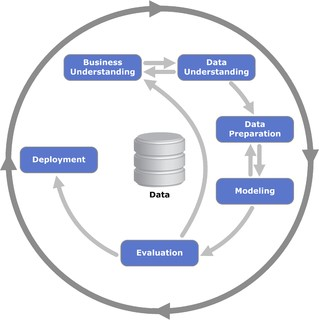
\includegraphics[width=0.46\textwidth,
                   height=0.32\textheight,
                   keepaspectratio]{images/CRISP-DM.jpg}
  \caption{Metodologi \textit{CRISP-DM}}
  \label{fig:crispdm}
\end{figure}

Metodologi pelaksanaan tugas akhir ini mengadopsi kerangka kerja CRISP-DM\label{abbr:CRISPDM} (\textit{Cross-Industry Standard Process for Data Mining}) untuk tahapan pengolahan data dan analitik. Pendekatan ini dipilih agar proses penelitian berjalan secara iteratif, fleksibel, dan tetap sistematis dalam menyelesaikan permasalahan yang telah dirumuskan.

\textbf{CRISP-DM} (\textit{Cross-Industry Standard Process for Data Mining}) adalah metodologi standar lintas industri untuk penambangan data yang menyediakan pendekatan terstruktur dalam enam fase utama, yaitu pemahaman bisnis (\textit{business understanding}), pemahaman data (\textit{data understanding}), persiapan data (\textit{data preparation}), pemodelan (\textit{modeling}), evaluasi (\textit{evaluation}), dan penyebaran (\textit{deployment}) (DataScience-PM, 2024). Metodologi ini bersifat iteratif, yang memungkinkan pengulangan fase jika diperlukan untuk meningkatkan kualitas hasil. Dalam penelitian ini, \textbf{CRISP-DM digunakan} untuk mengelola aspek penambangan data dan analitik prediktif.

\subsection{Tahapan Investigasi dan Pengumpulan Fakta}

Tahapan ini bertujuan untuk mengumpulkan data dan informasi faktual sebagai landasan perumusan masalah. Kegiatan yang dilakukan meliputi:

\begin{enumerate}[label=\alph*.]
  \item \textbf{Observasi sistem yang ada}, yaitu pengamatan terhadap sistem yang saat ini digunakan organisasi untuk mengidentifikasi keterbatasan dan kebutuhan pengguna internal.
  
  \item \textbf{Wawancara dengan pemangku kepentingan}, dilakukan secara terstruktur dengan perwakilan pemangku kepentingan internal untuk menggali kebutuhan fungsional dan ekspektasi terhadap sistem baru.
  
  \item \textbf{Analisis data historis}, dilakukan untuk menelaah volume dan tren permintaan, pola musiman, serta kelengkapan dan kualitas data yang tersedia.
  
  \item \textbf{Dokumentasi temuan}, mengompilasi seluruh hasil observasi, wawancara, dan analisis dalam bentuk laporan yang akan dilampirkan.
\end{enumerate}

\subsection{Studi Literatur}

Tahapan ini bertujuan untuk mengumpulkan, mengelompokkan, dan menyaring literatur yang relevan dengan topik penelitian. Proses yang dilakukan meliputi:

\begin{enumerate}[label=\alph*.]
  \item \textbf{Pencarian literatur sistematis} pada basis data akademik (IEEE Xplore, ScienceDirect, SpringerLink, ACM Digital Library, Google Scholar) menggunakan kata kunci terkait \textit{business intelligence}, \textit{chatbot}, \textit{natural language generation}, dan \textit{time series forecasting}. 
  
  \item \textbf{Pengelompokan literatur} berdasarkan tema utama, yaitu konsep \textit{Business Intelligence}, teknologi \textit{chatbot} dan \textit{conversational} AI, pemrosesan bahasa alami, metode peramalan deret waktu, integrasi sistem, dan studi kasus implementasi.
  
  \item \textbf{Penapisan dan analisis kualitas} literatur berdasarkan faktor dampak, jumlah sitasi, metodologi, dan relevansi terhadap penelitian.
  
  \item \textbf{Sintesis literatur} untuk membangun kerangka teoretis, mengidentifikasi praktik terbaik dan teknologi terkini, serta menyusun tinjauan pustaka pada Bab II.
  
  \item \textbf{Dokumentasi proses} dalam bentuk peninjauan penelitian terdahulu yang ditemukan dan membuat celah penelitian dan kontribusi besar yang ditawarkan penelitian ini.
\end{enumerate}

\subsection{Perancangan Sistem}

Tahapan ini meliputi perancangan arsitektur dan komponen sistem secara terperinci, mencakup:

\begin{enumerate}[label=\alph*.]
  \item \textbf{Perancangan arsitektur sistem}, yaitu penyusunan arsitektur berlapis yang mengintegrasikan \textit{chatbot}, pemrosesan bahasa alami, mesin \textit{rule-based query}, dan peramalan deret waktu, serta penentuan teknologi dan kerangka kerja yang akan digunakan.
  
  \item \textbf{Perancangan modul \textit{chatbot}}, meliputi komponen pemahaman bahasa alami (\textit{Natural Language Understanding}), manajemen dialog (\textit{Dialogue Management}), pembangkitan bahasa alami (\textit{Natural Language Generation}), serta pendefinisian \textit{intent} dan entitas yang akan dikenali.
  
  \item \textbf{Pengimplementasian \textit{rule-based query}}, yaitu pendefinisian aturan untuk kueri terstruktur dan berulang serta pemetaan antara \textit{intent} dengan templat kueri.
  
  \item \textbf{Perancangan model peramalan deret waktu}, meliputi penentuan variabel target, perancangan praolah data, pemilihan arsitektur model (ARIMA, Prophet, LSTM, dan GRU), perbandingan model statistik dengan model \textit{deep learning}, dan strategi evaluasi model.
  
  \item \textbf{Perancangan basis data dan gudang data}, yaitu perancangan skema basis data untuk menyimpan data pelanggan, hasil prediksi, dan data pelatihan NLP, serta perancangan proses ETL\label{abbr:ETL} (\textit{Extract, Transform, Load}).
  
  \item \textbf{Perancangan antarmuka pengguna}, meliputi pembuatan \textit{wireframe} dan \textit{mockup} untuk antarmuka \textit{chatbot}.
\end{enumerate}

\subsection{Implementasi Sistem}

Tahapan ini meliputi pengembangan sistem berdasarkan rancangan yang telah ditetapkan, mencakup:

\begin{enumerate}[label=\alph*.]
  \item \textbf{Pengembangan \textit{backend}}, yaitu implementasi mesin \textit{rule-based query}, model NLP untuk klasifikasi \textit{intent} dan pengenalan entitas, model peramalan deret waktu, serta penyediaan API\label{abbr:API} \textit{backend}.
  
  \item \textbf{Pengembangan \textit{frontend}}, meliputi implementasi antarmuka \textit{chatbot}.
  
  \item \textbf{Pengembangan basis data}, yaitu implementasi skema basis data, proses ETL untuk integrasi data, dan \textit{data pipeline} untuk pemrosesan data.
  
  \item \textbf{Integrasi komponen}, meliputi integrasi \textit{chatbot} dengan mesin \textit{rule-based query} dan NLP, integrasi model peramalan dengan sistem BI, serta implementasi mekanisme tembolok (\textit{caching}) untuk performa.
\end{enumerate}

\subsection{Pengujian dan Evaluasi}

Tahapan ini bertujuan menilai kinerja sistem secara menyeluruh, mencakup aspek fungsionalitas, akurasi, performa, dan kebergunaan.

\begin{enumerate}[label=\alph*.]
  \item \textbf{Pengujian unit}, yaitu setiap komponen diuji secara terpisah agar fungsinya terverifikasi dengan benar dan stabil.
  \item \textbf{Pengujian integrasi}, yaitu Interaksi antarmodul diverifikasi melalui skenario ujung-ke-ujung, dari masukan percakapan hingga keluaran berupa kueri yang dieksekusi, prediksi, narasi, dan visualisasi.
  \item \textbf{Pengujian fungsional}, yaitu Pemenuhan seluruh kebutuhan fungsional divalidasi menggunakan himpunan skenario representatif yang mencerminkan pertanyaan bisnis prioritas.
  \item \textbf{Evaluasi model NLP (klasifikasi intent multi\-kelas, satu label per ujaran)}, yaitu hasil dilaporkan sebagai \textit{top-1} dan \textit{top-k} accuracy; \textit{precision}, \textit{recall}, dan \textit{F1-score} per kelas yang kemudian dirata-ratakan dengan pendekatan \textit{macro}, \textit{micro}, dan \textit{weighted}. Disajikan pula \textit{confusion matrix} berukuran $K\times K$, evaluasi ambang kepercayaan untuk mekanisme \textit{fallback}/\texttt{UNKNOWN}, serta ringkasan kalibrasi probabilitas.
  \item \textbf{Evaluasi model peramalan deret waktu}, yaitu protokol yang digunakan ialah \textit{rolling-origin backtesting} pada beberapa horizon prediksi dengan \textit{seasonal naive} sebagai garis dasar. Laporan mencakup MAE\label{abbr:MAE}, RMSE\label{abbr:RMSE}, sMAPE\label{abbr:sMAPE}, dan MASE\label{abbr:MASE}, dilengkapi \textit{skill score} terhadap garis dasar. Hasil disajikan per horizon dan per entitas prioritas (median dan rentang antar kuartil).
  \item \textbf{Evaluasi performa sistem}, yaitu waktu respons, \textit{throughput}, dan latensi diukur pada beban realistis; \textit{load testing} dilakukan untuk menilai skalabilitas.
  \item \textbf{Evaluasi kebergunaan (\textit{usability})}, yaitu \textit{User Acceptance Testing} melibatkan sedikitnya 20–30 pengguna internal. Hasil dirangkum menggunakan skor \textit{System Usability Scale} (SUS)\label{abbr:SUS} dan umpan balik kualitatif terkait kemudahan, kejelasan, dan alur kerja.
\end{enumerate}

\subsection{Dokumentasi dan Penyusunan Laporan}

Tahapan akhir meliputi dokumentasi dan penyusunan laporan tugas akhir, mencakup:

\begin{enumerate}[label=\alph*.]
  \item \textbf{Dokumentasi teknis}, yaitu penyusunan dokumentasi API, dokumentasi kode, panduan pengguna (\textit{user manual}), dan panduan penyebaran (\textit{deployment guide}).
  
  \item \textbf{Penyusunan laporan tugas akhir}, meliputi penulisan laporan sesuai format yang ditetapkan dengan penyuntingan dan pemeriksaan kelengkapan.
  
  \item \textbf{Persiapan presentasi}, meliputi pembuatan \textit{slide} presentasi, penyusunan skenario demonstrasi sistem, dan kurasi materi pendukung.
  
  \item \textbf{Revisi dan finalisasi}, yaitu revisi berdasarkan masukan pembimbing, finalisasi laporan dan sistem, serta persiapan sidang tugas akhir.
\end{enumerate}

Seluruh proses metodologi ini akan didokumentasikan dengan baik untuk keterbukaan, kemampuan direproduksi, dan akuntabilitas penelitian.

\subsection{Sistematika Penulisan}

Laporan tugas akhir ini disusun dengan sistematika sebagai berikut.

\begin{enumerate}
  \item \textbf{Bab I Pendahuluan}: Berisi latar belakang, rumusan masalah, tujuan, batasan masalah, metodologi, dan sistematika penulisan laporan tugas akhir.
  \item \textbf{Bab II Studi Literatur}: Berisi kajian pustaka yang relevan dengan topik tugas akhir, mencakup teori dan konsep \textit{Business Intelligence}, \textit{chatbot} berbasis aturan, pemrosesan bahasa alami, pembangkitan bahasa alami, serta metode peramalan deret waktu.
  \item \textbf{Bab III Analisis}: Berisi analisis kebutuhan pengguna dan sistem, termasuk identifikasi pemangku kepentingan, kebutuhan fungsional dan non-fungsional, serta analisis data historis.
  \item \textbf{Bab IV Perancangan}: Berisi perancangan arsitektur sistem, modul \textit{chatbot} berbasis aturan, model peramalan, basis data, antarmuka pengguna, serta rencana implementasi dan evaluasi.
  \item \textbf{Bab V Implementasi}: Berisi penjelasan tentang proses implementasi seluruh komponen sistem, termasuk \textit{backend}, mesin aturan, klasifikasi maksud, pembangkitan bahasa alami, layanan \textit{machine learning}, \textit{frontend}, dan keamanan sistem.
  \item \textbf{Bab VI Evaluasi}: Berisi hasil pengujian fungsional, evaluasi akurasi model peramalan, analisis performa sistem, dan penilaian kebergunaan oleh pengguna internal.
  \item \textbf{Bab VII Kesimpulan dan Saran}: Berisi kesimpulan dari hasil pelaksanaan tugas akhir dan saran untuk pengembangan lebih lanjut.
  \item \textbf{Daftar Pustaka}: Berisi daftar referensi yang digunakan dalam penyusunan laporan tugas akhir.
  \item \textbf{Lampiran}: Berisi dokumen pendukung seperti transkrip wawancara, data pengujian, dan kode program.
\end{enumerate}



% \cleardoublepage % memastikan bab baru dimulai di halaman ganjil (kanan)
% \chapter{PENDAHULUAN}
% \label{chap:pendahuluan}
% % --- Latar Belakang ---
% \section{Latar Belakang}
% Subbab ini menjelaskan dasar pemikiran, motivasi, kebutuhan, alasan, atau urgensi pemilihan masalah tugas akhir. Subbab ini berisi penjelasan ringkas tentang kondisi atau situasi yang ada saat ini terkait dengan topik yang dibahas. Tujuan utamanya adalah untuk memberikan informasi secukupnya kepada pembaca agar memahami topik yang akan dibahas. Dalam subbab ini, jelaskan hal-hal berikut ini:
% \begin{enumerate}
% \item	Kondisi atau situasi topik yang dibahas beserta permasalahannya, misalnya tentang pengelolaan informasi di fasilitas kesehatan daerah pedesaan saat ini dan masalah yang dihadapi, berdasarkan hasil survei atau wawancara dengan pihak terkait.
% \item	Urgensi atau pentingnya penyelesaian masalah tersebut, misalnya dampak negatif yang ditimbulkan jika masalah tersebut tidak diselesaikan.
% \item	Berbagai solusi yang telah diterapkan maupun solusi yang memungkinkan untuk diterapkan untuk menyelesaikan masalah tersebut, berdasarkan hasil studi literatur, wawancara dengan pihak terkait, atau kunjungan lapangan.
% \item   Kelemahan atau kekurangan dari solusi yang telah diterapkan atau yang memungkinkan untuk diterapkan tersebut, yang menjadi dasar pemikiran dalam merumuskan masalah tugas akhir.
% \end{enumerate}
% Latar belakang dapat ditulis dalam 2-3 halaman. Penulisan latar belakang masalah yang baik akan mengantarkan pembaca kepada pemahaman yang jelas tentang topik yang akan dibahas, 
% sehingga pembaca dapat mengikuti pembahasan pada subbab-subbab berikutnya dengan baik. Oleh karena itu, 
% penulis diharapkan melakukan investigasi yang mendalam untuk mengumpulkan fakta-fakta yang relevan dengan topik yang dibahas, 
% baik melalui studi literatur, wawancara dengan pihak terkait, maupun kunjungan lapangan. Hasil studi ini dijelaskan secara \emph{ringkas} di dalam subbab ini.
% Penjelasan hasil studi literatur yang komprehensif dapat dijabarkan di Bab II Studi Literatur secara sistematis.

% Dalam menulis latar belakang, hindari penulisan yang bersifat terlalu umum atau terlalu luas cakupannya sehingga sulit untuk dihubungkan dengan topik yang dibahas dalam tugas akhir,
% seperti:
% \begin{enumerate}
%     \item "Pentingnya teknologi informasi dalam kehidupan manusia."
%     \item "Perkembangan pesat teknologi \emph{artificial intelligence} di era digital."
%     \item "Tantangan dalam pengelolaan data besar (\emph{big data}) di berbagai sektor industri."
%     \item "Peran teknologi informasi dalam meningkatkan kualitas layanan kesehatan."
% \end{enumerate}
% Penulisan yang terlalu umum atau luas cakupannya akan menyulitkan penulis dalam merumuskan masalah, tujuan, metodologi, dan evaluasi tugas akhir.

% Jika ada referensi yang digunakan dalam penulisan latar belakang, cantumkan referensi tersebut dengan benar menggunakan \texttt{biblatex} sesuai dengan contoh penulisan kutipan dan daftar pustaka yang telah disediakan dalam template ini.
% Sebagai contoh, pada paragraf berikut ini terdapat kutipan dari dua referensi yang berbeda \autocite{laudon2020, pressman2019}. 
% Ada dua format penulisan sitasi yang dapat digunakan, yaitu format naratif dan format parentetik.
% Contoh penulisan kutipan dengan format naratif adalah sebagai berikut:
% \begin{displayquote}
% Menurut \textcite{laudon2020}, sistem informasi adalah kombinasi dari teknologi informasi dan aktivitas orang yang menggunakan teknologi tersebut untuk mendukung operasi dan manajemen organisasi.
% \end{displayquote}
% Contoh penulisan kutipan dengan format parentetik adalah sebagai berikut:
% \begin{displayquote}
%     Sistem informasi merupakan kombinasi dari teknologi informasi dan aktivitas orang yang menggunakan teknologi tersebut untuk mendukung operasi dan manajemen organisasi \autocite{laudon2020}.
% \end{displayquote}
% % --- Rumusan Masalah ---
% \section{Rumusan Masalah}
% Rumusan Masalah berisi masalah utama yang dibahas dalam tugas akhir. Rumusan masalah yang baik memiliki struktur sebagai berikut:
% \begin{enumerate}
% \item	Pokok persoalan dari kondisi atau situasi yang ada saat ini. Dengan kata lain, jelaskan kelemahan atau kekurangan dari kondisi, situasi, atau solusi yang dijelaskan pada latar belakang. Ini merupakan pokok rumusan masalah.
% \item	Elaborasi lebih lanjut urgensi penyelesaian masalah tersebut (mengapa penting untuk diselesaikan dan akibat yang dapat terjadi jika tidak diselesaikan).
% \item	Usulan singkat terkait dengan solusi yang ditawarkan untuk menyelesaikan persoalan.
% Penting untuk diperhatikan bahwa persoalan yang dideskripsikan pada subbab ini akan dipertanggungjawabkan di bab Evaluasi (apakah terselesaikan atau tidak).
% \end{enumerate}
% Hindari penulisan rumusan masalah yang terlalu umum atau terlalu luas cakupannya sehingga sulit untuk diselesaikan dalam jangka waktu pelaksanaan tugas akhir, 
% seperti:
% \begin{enumerate}
%     \item "Bagaimana cara meningkatkan kualitas layanan kesehatan di Indonesia?"
%     \item "Bagaimana cara mengoptimalkan penggunaan energi di perkotaan?"
%     \item "Bagaimana cara mengurangi kemacetan lalu lintas di kota besar?"
%     \item "Bagaimana cara membangun sistem irigasi sawah menggunakan \emph{AI}?"
% \end{enumerate}
% Rumusan masalah yang baik dan spesifik akan memudahkan penulis dalam menentukan tujuan, metodologi, dan evaluasi tugas akhir.

% Selain itu, hindari menuliskan pertanyaan yang merupakan sebuah keniscayaan yang harus dijawab atau dikerjakan 
% dalam pelaksanaan tugas akhir, seperti:
% \begin{enumerate}
%     \item "Bagaimana cara melakukan analisis kebutuhan sistem informasi rumah sakit?"
%     \item "Bagaimana cara merancang basis data untuk aplikasi X?"
%     \item "Bagaimana cara mengimplementasikan \textit{large language model} untuk deteksi penyakit Y?"
%     \item "Bagaimana cara menguji sistem penyiraman tanaman berbasis IoT yang akan dibuat?"
% \end{enumerate}
% Kegiatan analisis, perancangan, implementasi, dan pengujian merupakan tahapan yang harus dilakukan dalam pelaksanaan tugas akhir,
% sehingga pertanyaan-pertanyaan tersebut tidak perlu dimasukkan ke dalam rumusan masalah.

% % --- Tujuan ---
% \section{Tujuan}
% Tuliskan \textbf{tujuan utama} dan/atau tujuan detail yang akan dicapai dalam pelaksanaan tugas akhir. 
% Fokuskan isi subbab ini pada hasil akhir yang ingin diperoleh setelah tugas akhir diselesaikan 
% terkait dengan penyelesaian persoalan pada rumusan masalah. 
% Penting untuk diperhatikan bahwa tujuan yang dideskripsikan pada subbab ini akan dipertanggungjawabkan 
% di akhir pelaksanaan tugas akhir. Oleh karena itu, tuliskan juga \emph{kriteria keberhasilan} tugas akhir ini.

% % --- Batasan Masalah ---
% \section{Batasan Masalah}
% Tuliskan batasan-batasan yang diambil dalam pelaksanaan tugas akhir. Batasan ini dapat dihindari (bersifat opsional, tidak perlu ada) jika topik atau judul tugas akhir dibuat cukup spesifik.

% % --- Metodologi Pengerjaan TA ---
% \section{Metodologi}
% Tuliskan semua tahapan yang akan dilalui selama pelaksanaan tugas akhir. 
% Tahapan ini spesifik untuk menyelesaikan persoalan tugas akhir. 
% Berikut adalah contoh metodologi pengerjaan tugas akhir yang dapat diikuti, yaitu meliputi tahapan, langkah-langkah, 
% atau tata cara melakukan:
% \begin{enumerate}
% \item	Investigasi pengumpulan fakta di latar belakang untuk merumuskan masalah.
% \item	Pencarian, pengelompokan, dan penapisan literatur atau sumber informasi untuk mengumpulkan informasi yang relevan tentang topik yang diangkat, termasuk teori (konsep atau teori apa saja yang perlu dicari), hal-hal yang telah dicapai oleh orang lain (cara mencari dan kata kuncinya), dan berbagai informasi pendukung, untuk mencari solusi terhadap masalah yang dibahas. Gunakan metodologi yang tepat dalam menggali informasi dan dokumentasikan prosesnya (termasuk rekaman wawancara atau survei) di dalam Lampiran, termasuk tautan ke video atau foto. Hasil penggalian informasi ini akan dijelaskan secara sistematis di Bab II Studi Literatur.
% \item   Analisis kebutuhan pengguna dan sistem berdasarkan hasil investigasi dan studi literatur. Jelaskan metode yang digunakan untuk melakukan analisis kebutuhan, misalnya wawancara, survei, observasi, atau studi kasus. Hasil analisis kebutuhan ini akan dijelaskan secara rinci di Bab III Analisis.
% \item   Perancangan solusi berdasarkan hasil analisis kebutuhan. Jelaskan metode yang digunakan untuk melakukan perancangan, misalnya menggunakan diagram UML, ERD, atau prototyping. Hasil perancangan ini akan dijelaskan secara rinci di Bab IV Perancangan.
% \item   Implementasi solusi berdasarkan hasil perancangan. Jelaskan teknologi, bahasa pemrograman, atau alat yang digunakan untuk mengimplementasikan solusi. Hasil implementasi ini akan dijelaskan secara rinci di Bab V Implementasi.
% \item   Evaluasi terhadap solusi yang telah diimplementasikan. Jelaskan metode pengujian, metrik evaluasi, atau studi kasus yang digunakan untuk menilai keberhasilan solusi. Hasil evaluasi ini akan dijelaskan secara rinci di Bab VI Evaluasi.
% \item   Penarikan kesimpulan dan saran berdasarkan hasil pelaksanaan tugas akhir. Hasil kesimpulan dan saran ini akan dijelaskan secara rinci di Bab VII Kesimpulan dan Saran. 
% \vfill % memaksa konten di atas untuk berada di bagian atas halaman dan menyisakan ruang kosong di bawah konten ini akibat berakhirnya section ini
% \end{enumerate}

% % --- Sistematika Penulisan ---
% \section{Sistematika Penulisan}
% Tuliskan gambaran umum isi dari setiap bab yang ada dalam laporan tugas akhir. Sistematika penulisan ini memberikan panduan bagi pembaca tentang struktur dan alur pembahasan dalam laporan tugas akhir. Berikut adalah contoh sistematika penulisan yang dapat diikuti:
% \begin{enumerate}
% \item	Bab I Pendahuluan: Berisi latar belakang, rumusan masalah, tujuan, batasan masalah, metodologi, dan sistematika penulisan laporan tugas akhir       .
% \item	Bab II Studi Literatur: Berisi kajian pustaka yang relevan dengan topik tugas akhir, termasuk teori-teori, konsep-konsep, dan hasil-hasil penelitian sebelumnya yang                mendukung pelaksanaan tugas akhir.
% \item	Bab III Analisis: Berisi penjelasan tentang analisis masalah dan kebutuhan pengguna serta berbagai alternatif solusinya.
% \item   Bab IV Perancangan: Berisi penjelasan tentang perancangan solusi yang diusulkan, misalnya arsitektur sistem, desain basis data, antarmuka pengguna, dan sebagainya.
% \item	Bab V Implementasi: Berisi penjelasan tentang proses implementasi solusi yang diusulkan, termasuk langkah-langkah yang diambil, teknologi yang digunakan, dan hasil yang diperoleh.
% \item	Bab VI Evaluasi: Berisi analisis dan evaluasi terhadap solusi yang diimplementasikan, termasuk metode pengujian, hal-hal yang disiapkan sebelum pengujian, hasil pengujian, dan penilaian kinerja.                  
% \item   Bab VII Kesimpulan dan Saran: Berisi kesimpulan dari hasil pelaksanaan tugas akhir dan saran untuk pengembangan lebih lanjut.
% \item   Daftar Pustaka: Berisi daftar referensi yang digunakan dalam penyusunan laporan tugas akhir.
% \item   Lampiran: Berisi dokumen-dokumen pendukung seperti kode program, data lengkap hasil pengujian, rekaman wawancara, dan lain-lain. 
% \end{enumerate}

% ==============================================================================
% BAB II - STUDI LITERATUR 
% ==============================================================================

\chapter{STUDI LITERATUR}
\label{chap:studi-literatur}

Bab ini menyajikan kajian teoretis dan tinjauan pustaka yang relevan dengan topik penelitian. Pembahasan meliputi konsep \textit{Business Intelligence}, teknologi \textit{chatbot} dan \textit{Conversational AI}, klasifikasi \textit{intent} berbasis pola, pembangkitan bahasa alami berbasis templat, serta peramalan deret waktu yang mendukung analisis dan prediksi permintaan layanan pelanggan. Kajian literatur ini disusun secara sistematis untuk memberikan landasan teoretis yang kuat bagi pengembangan sistem yang diusulkan, dengan fokus pada integrasi \textit{pattern-based intent classification}, \textit{template-based natural language generation}, dan \textit{time series forecasting} dalam satu platform terintegrasi.

% ==============================================================================
\section{\textit{Business Intelligence} dan Arsitektur Sistem}
% ==============================================================================

Bagian ini membahas konsep dasar \textit{Business Intelligence}, evolusinya, serta arsitektur sistem yang mendukung implementasi BI modern. Pembahasan mencakup komponen-komponen utama arsitektur BI dan peran \textit{semantic layer} dalam menjembatani kesenjangan antara data teknis dan kebutuhan bisnis. Pemahaman yang komprehensif tentang arsitektur BI menjadi fondasi penting dalam merancang sistem yang mampu mengintegrasikan berbagai komponen teknologi secara efektif.

\subsection{Konsep \textit{Business Intelligence}}

\textit{Business Intelligence} (BI) merupakan sistem teknologi yang mengumpulkan, mengorganisasi, dan menganalisis data dari berbagai sumber dalam suatu bisnis untuk membantu perusahaan mengubah data mentah menjadi wawasan yang berguna sehingga mereka dapat membuat keputusan yang lebih baik \autocite{sorour2020business}. Evolusi BI dari sistem berbasis aturan tradisional ke platform berbasis kecerdasan buatan telah meningkatkan secara signifikan analitik prediktif, otomatisasi, dan kemampuan pengambilan keputusan waktu nyata di seluruh industri \autocite{khaddam2025ai}.

Implementasi BI di institusi pendidikan tinggi telah menunjukkan kemampuan untuk memantau aktivitas jaminan kualitas dan mendukung pengambilan keputusan strategis \autocite{sorour2020business}. Penelitian empiris menunjukkan bahwa organisasi yang mengadopsi pengambilan keputusan berbasis data secara sistematis memperoleh keunggulan produktivitas yang signifikan dibandingkan organisasi yang belum mengadopsinya \autocite{Brynjolfsson2016DDD}. Pasar BI global terus menunjukkan pertumbuhan yang signifikan, dengan proyeksi mencapai USD 116,25 miliar pada tahun 2033 dari USD 36,82 miliar pada tahun 2025, dengan CAGR sebesar 14,98\% \autocite{Straits2024}. Pertumbuhan ini menunjukkan relevansi dan kebutuhan akan solusi BI yang inovatif dalam menghadapi kompleksitas data bisnis modern.

\subsection{Arsitektur \textit{Business Intelligence} Hibrida}

Arsitektur BI hibrida mengintegrasikan sistem BI tradisional dengan kemampuan kecerdasan buatan untuk meningkatkan pengambilan keputusan, analitik prediktif, dan efisiensi operasional. Pendekatan ini menyajikan struktur yang memanfaatkan model pembelajaran mesin bersama pelaporan BI tradisional untuk menjembatani kesenjangan antara analisis historis dan wawasan berbasis data waktu nyata \autocite{Torres2018BIPerformance}.

Komponen utama arsitektur BI hibrida mencakup beberapa lapisan yang saling terintegrasi \autocite{Torres2018BIPerformance}. Lapisan sumber data mencakup sumber internal seperti sistem CRM dan perangkat lunak keuangan, serta sumber eksternal seperti data media sosial dan laporan pasar. Gudang data berfungsi sebagai fasilitas penyimpanan terpusat untuk data yang terorganisasi dan siap digunakan untuk pelaporan. Mesin analitik bertanggung jawab untuk pengenalan pola dan analisis tren, memberikan wawasan prediktif untuk perencanaan strategis. Lapisan visualisasi menyediakan dashboard interaktif dan laporan yang meningkatkan adopsi pengguna melalui presentasi data yang intuitif.

Penelitian empiris berskala besar menunjukkan bahwa organisasi yang mengadopsi pengambilan keputusan berbasis data (\textit{data-driven decision-making}) memiliki produktivitas 5--6\% lebih tinggi dibandingkan organisasi yang belum mengadopsinya \autocite{Brynjolfsson2016DDD}. Studi lain mengonfirmasi bahwa kapabilitas \textit{Business Intelligence} dan analitik berdampak positif terhadap kinerja organisasi melalui peningkatan kemampuan perubahan proses bisnis \autocite{Torres2018BIPerformance}. Integrasi komponen-komponen ini membentuk fondasi yang kuat untuk sistem BI modern yang responsif dan dapat diandalkan.

\subsection{\textit{Semantic Layer} dalam \textit{Business Intelligence}}

\textit{Semantic layer} adalah antarmuka berorientasi bisnis yang menjembatani kesenjangan antara model data yang kompleks dan pengguna bisnis, bertindak sebagai lapisan abstraksi yang menerjemahkan struktur data teknis ke dalam istilah dan konsep bisnis yang familiar \autocite{databricks2025semantic}. Lapisan semantik menyediakan pandangan bisnis terpadu terhadap data di seluruh organisasi, terlepas dari lokasi data atau bagaimana secara teknis terstruktur.

Lapisan semantik menyederhanakan konsep dan teknis data untuk pengguna bisnis sehingga mereka tidak perlu mengubah data bisnis yang mendasarinya untuk bekerja dengan cara baru \autocite{atscale2025semantic}. Lapisan ini memungkinkan pengguna bisnis untuk berinteraksi dengan data menggunakan terminologi yang mereka pahami tanpa perlu memahami struktur teknis basis data yang mendasarinya. Kemampuan ini sangat penting dalam konteks sistem \textit{chatbot} BI, dengan memfasilitasi interpretasi kueri bahasa alami menjadi operasi basis data yang sesuai.

\subsubsection{Komponen Inti \textit{Semantic Layer}}

Lapisan semantik memiliki lima komponen inti yang bertindak sebagai fondasi struktural dan teknis \autocite{dbt2024semantic}. Komponen pertama adalah definisi model semantik yang menciptakan representasi logis dari domain bisnis, memetakan struktur basis data teknis ke konsep bisnis. Alih-alih bekerja dengan tabel mentah seperti \texttt{usr\_tbl} atau \texttt{trx\_hist}, entitas seperti \texttt{Customer} atau \texttt{Order} didefinisikan untuk merangkum kompleksitas yang mendasarinya.

Komponen kedua adalah manajemen metadata yang menangani informasi tentang data, seperti deskripsi bidang, garis keturunan data (\textit{data lineage}), frekuensi pembaruan, dan metrik kualitas. Lapisan logika bisnis sebagai komponen ketiga berisi aturan perhitungan spesifik untuk metrik bisnis. Komponen keempat adalah lapisan akses data yang menerjemahkan permintaan bisnis menjadi kueri basis data yang dioptimalkan, menerapkan filter keamanan yang diperlukan. Komponen terakhir adalah mekanisme \textit{caching} yang memeriksa apakah hasil perhitungan sudah tersedia dalam tembolok sebelum menjalankan kueri.

Implementasi \textit{semantic layer} yang efektif memungkinkan organisasi untuk mencapai konsistensi dalam pelaporan dan analisis, sekaligus mengurangi kompleksitas teknis yang dihadapi oleh pengguna bisnis. Pemahaman tentang \textit{semantic layer} ini menjadi dasar penting dalam merancang sistem klasifikasi \textit{intent} yang akan dibahas pada bagian selanjutnya.


\section{\textit{Rule-Based Query} dan Implementasinya pada \textit{Chatbot}}

\begin{figure}[t]
  \centering
  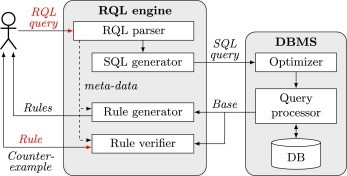
\includegraphics[width=0.46\textwidth,
                   height=0.32\textheight,
                   keepaspectratio]{images/rbq.jpg}
  \caption{Bahasa Kueri untuk Penemuan Aturan dalam Basis Data}
  \label{fig:rbq}
\end{figure}

\subsection{Konsep \textit{Rule-Based Query} dalam Sistem Basis Data}

Secara historis, optimisasi kueri pada sistem manajemen basis data relasional banyak mengandalkan pendekatan berbasis aturan (\textit{rule-based}) dan berbasis biaya (\textit{cost-based}) untuk memilih rencana eksekusi kueri yang efisien \autocite{Yang2024MLQueryOpt,Shah2025AIDB}. Pendekatan \textit{rule-based} menggunakan seperangkat aturan heuristik yang ditetapkan pakar (seperti yang diilustrasikan pada Gambar~\ref{fig:rbq}), seperti urutan penerapan seleksi dan proyeksi, penggunaan indeks, atau restrukturisasi \textit{join}, untuk menyederhanakan dan mengoptimalkan kueri tanpa melakukan estimasi biaya numerik yang rinci \autocite{Yang2024MLQueryOpt}. Aturan-aturan tersebut, misalnya, dapat mengharuskan operator seleksi ditempatkan sedekat mungkin dengan sumber data atau menganjurkan penggunaan indeks ketika kondisi penyaringan sesuai sehingga mengurangi jumlah baris yang harus diproses pada tahap-tahap berikutnya.

Meskipun perkembangan terkini banyak mengarah pada optimisasi kueri berbasis kecerdasan buatan, sejumlah kajian menegaskan bahwa teknik berbasis aturan masih relevan dan sering digunakan sebagai fondasi, terutama untuk pola kueri yang berulang dan terstruktur dengan baik \autocite{Shah2025AIDB,Lubis2025ERDOpt}. Dalam konteks sistem \textit{Business Intelligence}, aturan-aturan kueri dapat dirancang untuk memetakan permintaan bisnis yang sering muncul (misalnya, ``total penjualan per bulan per segmen pelanggan'') ke pola kueri yang terstandarisasi terhadap gudang data sehingga mempercepat proses pengambilan data dan menjaga konsistensi hasil analisis.

\subsection{\textit{Chatbot} Berbasis Aturan dan Pencocokan Pola}

Pada ranah \textit{chatbot}, pendekatan berbasis aturan (\textit{rule-based chatbot}) merupakan salah satu arsitektur paling awal dan masih banyak digunakan untuk skenario tugas-terarah (\textit{task-oriented}) dengan ruang lingkup percakapan yang terbatas \autocite{Singh2025ChatbotsSurvey,Ouali2024ArabicChatbots}. \textit{Chatbot} berbasis aturan umumnya bekerja dengan mencocokkan masukan pengguna terhadap pola-pola teks yang telah didefinisikan sebelumnya menggunakan teknik pencocokan pola (\textit{pattern matching}), pencarian kata kunci, atau ekspresi reguler. Ketika suatu pola terpenuhi, sistem akan mengeksekusi aturan yang terkait, baik berupa pemilihan respons templat maupun pemanggilan prosedur tertentu di \textit{backend}.

Kajian sistematis mengenai \textit{chatbot} berbahasa Arab menunjukkan bahwa pendekatan \textit{pre-scripted rules} memetakan ujaran pengguna ke aturan atau pola yang telah dipersiapkan, kemudian memilih respons dari himpunan jawaban yang sudah tersedia \autocite{Ouali2024ArabicChatbots}. Pendekatan ini juga digunakan pada berbagai \textit{chatbot} klasik seperti ELIZA dan ALICE, serta pada bahasa skrip khusus seperti AIML (\textit{Artificial Intelligence Markup Language}) yang memungkinkan pengembang mendefinisikan pola masukan dan templat keluaran secara eksplisit \autocite{Singh2025ChatbotsSurvey}. Keunggulan utama pendekatan berbasis aturan terletak pada kontrol penuh terhadap perilaku sistem, kemudahan untuk menjamin bahwa respons tidak keluar dari batas pengetahuan yang diizinkan, serta kesesuaian untuk domain yang sangat terstruktur.

Penelitian terbaru di Indonesia juga mengimplementasikan pendekatan pencocokan pola berbasis aturan untuk mengembangkan \textit{chatbot} layanan informasi internal. Misalnya, pengembangan aplikasi Sido \textit{chatbot} menggunakan pola aturan dan pencocokan pola untuk menjawab pertanyaan umum pengguna, disertai pengujian keberhasilan respons melalui uji fungsional dan kuesioner pengguna \autocite{Ananta2025SidoChatbot}. Studi lain mengimplementasikan kerangka kerja Rasa untuk membangun sistem \textit{FAQ bot} yang menggabungkan pemetaan intent dengan aturan dialog dan integrasi ke platform pesan seperti Telegram, menunjukkan bahwa arsitektur hibrida berbasis aturan dan pembelajaran mesin dapat memberikan fleksibilitas sekaligus menjaga struktur dialog yang terkontrol \autocite{Talenggoran2025RasaFAQ}.

\subsection{Integrasi \textit{Rule-Based Query} dalam Arsitektur Chatbot BI}

Dalam konteks \textit{Business Intelligence}, beberapa kajian mengusulkan penggunaan \textit{chatbot} sebagai antarmuka percakapan untuk eksplorasi data dan kolaborasi analitik, dengan komponen percakapan (\textit{conversational agent}) bekerja berdampingan dengan agen eksplorasi data dan agen rekomendasi \autocite{Cherednichenko2023CBIRefModel}. Pendekatan ini sering kali memanfaatkan arsitektur berbasis aturan untuk menerjemahkan permintaan dalam bahasa alami menjadi perintah atau kueri terstruktur terhadap sistem BI dan gudang data. Aturan-aturan tersebut dapat mencakup pemetaan intent tertentu ke templat kueri, pengisian parameter kueri dari entitas yang diekstraksi, serta penentuan agregasi dan dimensi pelaporan berdasarkan frasa waktu atau hierarki bisnis yang disebutkan pengguna.

\textit{Chatbot} berbasis aturan memerlukan basis pengetahuan yang menyimpan aturan-aturan yang dirancang secara manual untuk menjamin kekokohan dan konsistensi perilaku sistem \autocite{Singh2025ChatbotsSurvey}. Dalam kerangka \textit{chatbot} BI, basis pengetahuan ini tidak hanya berisi pasangan pola–jawaban, tetapi juga aturan pemetaan ke \textit{rule-based query engine} yang mengakses gudang data. Studi-studi tersebut mendukung pendekatan yang digunakan dalam penelitian ini, yaitu menggabungkan klasifikasi intent berbasis pola dengan \textit{rule-based query} yang terdokumentasi dengan baik sehingga sistem dapat menjawab pertanyaan bisnis terstruktur secara andal dan transparan, sembari tetap membuka ruang pengembangan lebih lanjut untuk integrasi teknik pembelajaran mesin yang lebih canggih jika cakupan intent dan kompleksitas kebutuhan analitik meningkat.


% ==============================================================================
\section{\textit{Pattern-Based Intent Classification} dengan \textit{Confidence Level}}
% ==============================================================================
\begin{figure}[t]
  \centering
  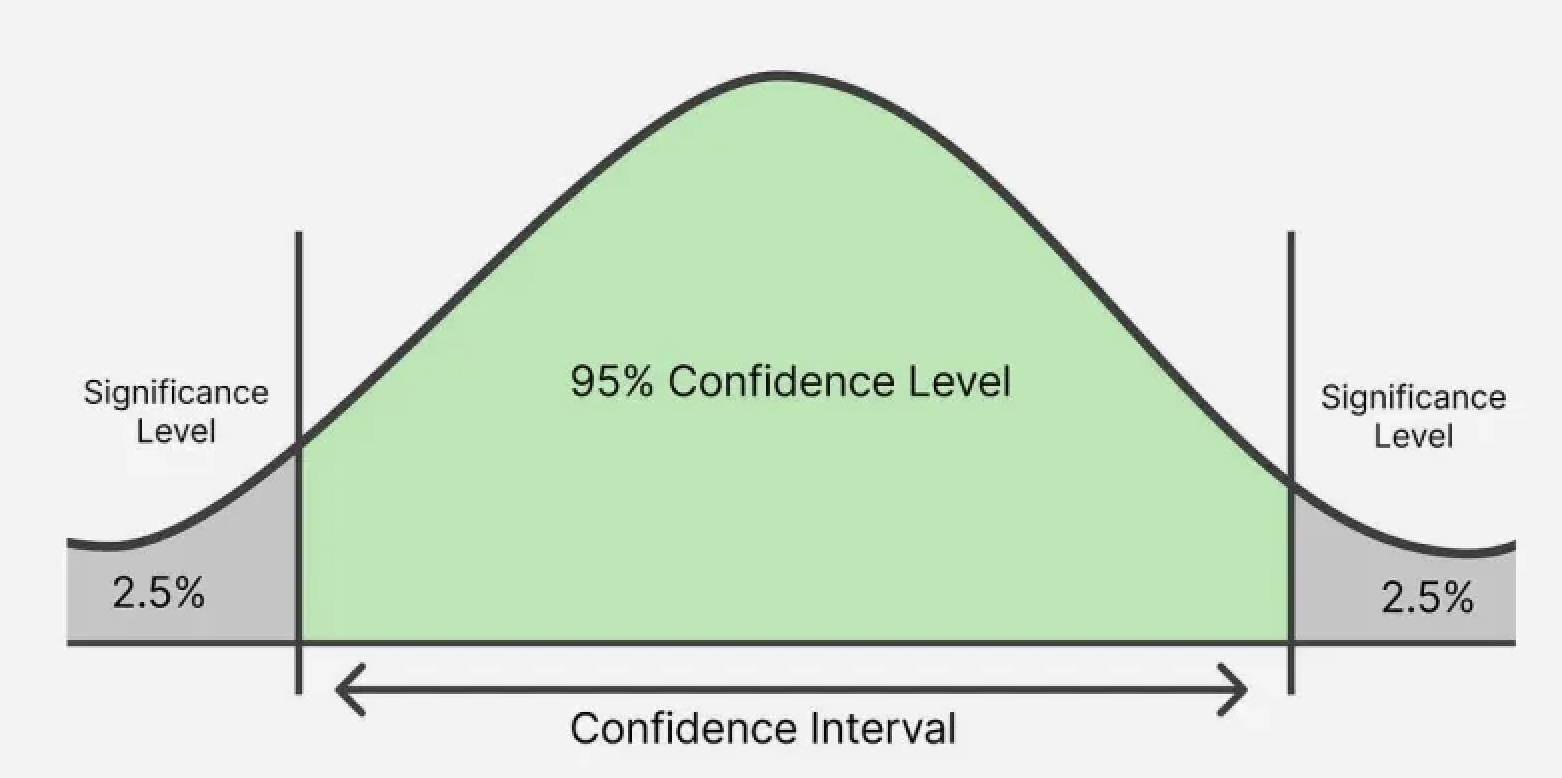
\includegraphics[width=0.46\textwidth,
                   height=0.32\textheight,
                   keepaspectratio]{images/pbi.png}
  \caption{\textit{Pattern-Based Intent Classification}}
  \label{fig:pbi}
\end{figure}
Bagian ini membahas pendekatan klasifikasi \textit{intent} berbasis pola untuk sistem \textit{chatbot} (seperti yang ditunjukkan pada Gambar~\ref{fig:pbi}), dengan fokus pada mekanisme pencocokan pola, penggunaan \textit{confidence score}, dan evaluasi performa. Klasifikasi \textit{intent} merupakan komponen kritis dalam memahami maksud pengguna dari kueri bahasa alami dan menentukan respons yang sesuai berdasarkan data internal perusahaan.

\subsection{Konsep \textit{Intent Classification}}

Klasifikasi \textit{intent} adalah proses menentukan niat atau tujuan pengguna dari masukan mereka, yang merupakan tugas fundamental dalam sistem \textit{chatbot} percakapan \autocite{ouaddi2025comparative}. Inti dari \textit{chatbot} berbasis AI adalah komponen NLU\label{abbr:NLU} yang mengklasifikasikan \textit{intent} pengguna untuk menghasilkan respons yang sesuai. Tugas klasifikasi ini sangat penting karena menentukan alur percakapan dan tindakan yang akan diambil sistem.

Pasar \textit{Conversational AI} global diproyeksikan mencapai USD 49,9 miliar pada tahun 2030, meningkat dari USD 10,7 miliar pada tahun 2023, dengan CAGR sebesar 25,2\% \autocite{Qaltivate2025}. Pertumbuhan eksponensial ini didorong oleh meningkatnya adopsi teknologi AI dalam layanan pelanggan dan operasional bisnis. Penelitian menunjukkan bahwa \textit{chatbot} berbasis AI mampu menangani sebagian besar pertanyaan rutin pelanggan secara otomatis, sehingga mengurangi beban kerja agen manusia dan mempercepat waktu respons secara signifikan \autocite{Adam2021Chatbots}. Temuan ini menunjukkan potensi besar klasifikasi \textit{intent} dalam meningkatkan efisiensi operasional dan kepuasan pengguna.

\subsection{Pertimbangan Alternatif: Klasifikasi \textit{Intent} Berbasis \textit{Transformer}}

Klasifikasi \textit{intent} berbasis \textit{Transformer} merupakan pendekatan modern yang memanfaatkan mekanisme perhatian diri (\textit{self-attention}) untuk memahami konteks ujaran pengguna secara dua arah. Model-model seperti BERT, RoBERTa, dan IndoBERT telah menunjukkan kinerja unggul pada tugas klasifikasi \textit{intent}, termasuk dalam bahasa Indonesia dengan akurasi mencapai sekitar 0{,}94 \autocite{Merugu2024IntentLLM,Ozerova2022IntentModule,Gehweiler2024IntentModeration}. Namun, literatur juga menyoroti adanya kompromi antara kualitas prediksi, latensi sistem, dan konsumsi sumber daya komputasi yang signifikan \autocite{Merugu2024IntentLLM,Gehweiler2025IntentSurvey}.

Pendekatan ini tidak diimplementasikan pada prototipe sistem dalam penelitian ini dengan tiga pertimbangan utama: (1) ruang lingkup pertanyaan yang relatif terbatas pada kebutuhan analitik internal, (2) pola kueri pengguna yang cenderung berulang dan terstruktur, serta (3) prioritas efisiensi komputasi tanpa ketergantungan pada unit pemroses grafis (GPU) berbiaya tinggi \autocite{Ozerova2022IntentModule}. Sebagai gantinya, penelitian ini mengadopsi pendekatan berbasis pola (\textit{pattern matching}) dengan mekanisme nilai keyakinan yang dibahas pada subbab berikutnya, dan menjadikan pendekatan berbasis \textit{Transformer} sebagai rekomendasi pengembangan lanjutan di masa mendatang.

\subsection{\textit{Pattern Matching} untuk \textit{Intent Classification}}

Pendekatan berbasis pola (\textit{pattern matching}) dalam klasifikasi \textit{intent} menggunakan aturan dan templat yang telah ditentukan sebelumnya untuk mencocokkan masukan pengguna dengan kategori \textit{intent} yang sesuai. Sistem ini menyimpan pola-pola pertanyaan atau \textit{utterances} untuk setiap \textit{intent}, kemudian membandingkan \textit{input} pengguna dengan pola-pola yang telah didefinisikan untuk menemukan kecocokan terbaik.

Pendekatan \textit{pattern matching} efektif untuk menangani kueri terstruktur dan berulang dalam domain spesifik. Implementasi dapat dilakukan menggunakan ekspresi reguler, pencocokan \textit{n-gram}, atau algoritma kesamaan string seperti \textit{Fuzzy String Matching} \autocite{mulyatun2021chatbot}. Keuntungan utama pendekatan ini adalah kecepatan eksekusi yang tinggi, prediktabilitas hasil, dan kontrol penuh atas logika pencocokan, menjadikannya pilihan yang tepat untuk sistem yang memerlukan respons cepat dan deterministic based pada data internal perusahaan.

\subsection{\textit{Confidence Score} dalam \textit{Intent Classification}}

\textit{Confidence score} atau skor keyakinan adalah nilai numerik antara 0 dan 1 yang menunjukkan tingkat kepercayaan sistem terhadap prediksi klasifikasi \textit{intent} \autocite{khosla2022evaluating}. Skor ini dihitung berdasarkan tingkat kecocokan antara \textit{input} pengguna dengan pola yang telah didefinisikan. Semakin tinggi kecocokan, semakin tinggi nilai \textit{confidence score}, dan semakin besar kemungkinan respons yang diberikan adalah benar.

Sistem menghitung \textit{confidence score} dengan membandingkan \textit{input} pengguna terhadap semua pola \textit{utterances} atau frasa pelatihan yang tersedia. Sistem kemudian memilih \textit{intent} dengan skor tertinggi sebagai prediksi. Implementasi \textit{confidence score} memungkinkan sistem untuk mengidentifikasi kapan prediksi mungkin tidak akurat dan memerlukan mekanisme \textit{fallback} \autocite{kuligowska2024enhancing}.

\subsubsection{\textit{Confidence Threshold}}

\textit{Confidence threshold} adalah nilai ambang batas minimum yang harus dicapai oleh \textit{confidence score} agar sistem memicu respons \textit{intent} tertentu. Dalam literatur, nilai \textit{threshold} umumnya dinyatakan sebagai angka numerik antara 0 dan 1; sebagai rujukan, nilai \textit{default} yang lazim digunakan pada \textit{framework} klasifikasi \textit{intent} adalah sekitar 0,45 \autocite{hengst2024conformal}, sedangkan sistem yang lebih konservatif dapat menggunakan \textit{threshold} yang lebih tinggi untuk mengurangi risiko respons yang salah. Perlu dicatat bahwa skala dan nilai ambang aktual yang digunakan pada suatu sistem bergantung pada rancangan mekanisme \textit{scoring}-nya; konversi antara skala 0--1 dan skala 0--100 dilakukan dengan mengalikan atau membagi nilai dengan 100.

Jika \textit{confidence score} terbaik jatuh di bawah threshold, sistem akan memicu interaksi \textit{fallback}, biasanya berupa pesan yang meminta klarifikasi atau memberitahu pengguna bahwa sistem tidak memahami pertanyaan. Pengaturan \textit{threshold} yang tepat sangat penting untuk menyeimbangkan antara tingkat otomasi dan akurasi respons \autocite{cyara2024optimum}.

Analisis \textit{threshold} membantu menentukan pengaturan yang optimal berdasarkan \textit{Key Performance Indicators} (KPI)\label{abbr:KPI} bisnis. Organisasi dapat menyesuaikan \textit{threshold} berdasarkan tiga pendekatan utama. Pendekatan pertama adalah menyesuaikan \textit{threshold} untuk mencapai persentase target respons yang benar. Pendekatan kedua adalah membatasi persentase maksimal respons yang salah. Pendekatan ketiga adalah mengoptimalkan trade-off antara tingkat otomasi dan risiko kesalahan berdasarkan toleransi bisnis \autocite{cyara2024optimum,genesys2023threshold}.

\subsection{Evaluasi Performa \textit{Intent Classification}}

Evaluasi performa klasifikasi \textit{intent} dilakukan dengan mengukur beberapa metrik kunci yang mencerminkan akurasi dan keandalan sistem dalam memprediksi niat pengguna. Evaluasi yang komprehensif memastikan bahwa sistem dapat beroperasi sesuai dengan standar yang ditetapkan dan memberikan pengalaman pengguna yang optimal.

\subsubsection{Metrik Evaluasi Klasifikasi \textit{Intent} Multi-Kelas}

Pencocokan kueri pengguna ke aturan bisnis (\textit{business rule}) dalam penelitian ini dievaluasi menggunakan metrik standar yang disesuaikan untuk masalah klasifikasi multi-kelas. Sistem memiliki 38 aturan bisnis yang saling eksklusif---bukan 38 \textit{intent}; jumlah \textit{intent} (kategori maksud) adalah tujuh ditambah satu \textit{fallback}, sedangkan 38 adalah jumlah aturan analitik yang masing-masing memiliki fungsi \texttt{calculateConfidence} tersendiri. Pendekatan evaluasi harus mengakomodasi bahwa setiap kueri pengguna hanya dapat dipetakan ke satu aturan yang benar sehingga metrik klasifikasi biner harus diperluas menggunakan strategi \textit{one-vs-all} dan agregasi yang tepat \autocite{Grandini2020MultiClassMetrics,EvidentlyMultiClass}.

Perbedaan utama antara klasifikasi multi-kelas dan biner adalah pada interpretasi elemen matriks kebingungan (\textit{confusion matrix}) dan agregasi metrik per-kelas. Dalam 38 aturan bisnis, matriks kebingungan berukuran 38$\times$38, dengan setiap baris merepresentasikan aturan hasil prediksi dan setiap kolom merepresentasikan aturan sebenarnya. Prediksi yang benar terletak pada diagonal utama, sedangkan prediksi salah tersebar pada sel off-diagonal. Pola sebaran kesalahan pada matriks kebingungan multi-kelas memberikan wawasan berharga tentang persamaan atau kebingungan antar aturan, misalnya kueri yang seharusnya dipetakan ke aturan ``Total Order HSI'' yang justru terpetakan ke ``Tren Pertumbuhan Order'' menunjukkan kesamaan semantik kata kunci yang perlu ditangani dengan pola diferensiasi yang lebih spesifik \autocite{EvidentlyMultiClass}.

Dalam menghitung metrik per kelas-\(i\), masalah klasifikasi multi-kelas diubah menjadi masalah biner secara virtual melalui pendekatan \textit{one-vs-all} \autocite{Grandini2020MultiClassMetrics}:

\begin{enumerate}[label=\alph*.]
    \item \textbf{TP\textsubscript{i}} (\textit{True Positive}): Jumlah sampel kelas-\(i\) yang diprediksi benar sebagai kelas-\(i\) (elemen diagonal matriks kebingungan pada baris dan kolom \(i\))
    
    \item \textbf{FP\textsubscript{i}} (\textit{False Positive}): Jumlah sampel kelas selain \(i\) yang diprediksi sebagai kelas-\(i\) (jumlah seluruh baris \(i\) pada matriks kebingungan kecuali elemen diagonal)
    
    \item \textbf{FN\textsubscript{i}} (\textit{False Negative}): Jumlah sampel kelas-\(i\) yang diprediksi salah sebagai kelas lain (jumlah seluruh kolom \(i\) pada matriks kebingungan kecuali elemen diagonal)
\end{enumerate}

Dalam konteks agregasi metrik (\textit{macro-average} dengan \textit{micro-average}) dan adanya 38 aturan bisnis dalam sistem ini, diperlukan strategi agregasi untuk memperoleh metrik keseluruhan performa sistem. Dua pendekatan utama yang umum digunakan dalam klasifikasi multi-kelas adalah \textit{macro-averaging} dan \textit{micro-averaging} \autocite{EvidentlyMultiClass}

Pendekatan \textbf{\textit{Macro-Averaging}} ini menghitung metrik (\textit{Precision}, \textit{Recall}, \textit{F1-Score}) untuk setiap aturan secara individual, kemudian mengambil rata-rata aritmatik dari 38 nilai metrik tersebut. Strategi ini memberikan bobot yang sama untuk setiap kelas sehingga mengutamakan performa pada kelas minoritas dan mencegah kelas mayoritas mendominasi hasil evaluasi \autocite{Grandini2020MultiClassMetrics}.

\phantomsection\label{sym:sum}
\begin{align}
\text{Presisi}_{\text{makro}} &= \frac{1}{38}\sum_{i=1}^{38} \text{Presisi}_i \\
\text{Daya Ingat}_{\text{makro}} &= \frac{1}{38}\sum_{i=1}^{38} \text{Daya Ingat}_i \\
\text{Skor-F1}_{\text{makro}} &= \frac{1}{38}\sum_{i=1}^{38} \text{Skor-F1}_i
\end{align}
\eqcaption{Makro-Rata Presisi, Daya Ingat, dan Skor-F1}

Pendekatan \textbf{\textit{Micro-Averaging}} menjumlahkan seluruh nilai TP, FP, dan FN dari semua kelas terlebih dahulu, kemudian menghitung metrik secara global berdasarkan jumlahan tersebut. Strategi ini memberikan bobot yang sama untuk setiap sampel sehingga metrik cenderung didominasi oleh kelas mayoritas dan mengabaikan performa pada kelas minoritas. Dalam klasifikasi multi-kelas, mikro-rata presisi = mikro-rata daya ingat = akurasi\autocite{EvidentlyMultiClass}.

\begin{align}
\text{Presisi}_{\text{mikro}} &= \frac{\sum_{i=1}^{38} \text{TP}_i}{\sum_{i=1}^{38} (\text{TP}_i + \text{FP}_i)} \\
\text{Daya Ingat}_{\text{mikro}} &= \frac{\sum_{i=1}^{38} \text{TP}_i}{\sum_{i=1}^{38} (\text{TP}_i + \text{FN}_i)}
\end{align}
\eqcaption{Mikro-Rata Presisi dan Daya Ingat}

Sebagai pendekatan komplementer, rata-rata tertimbang menghitung metrik per-kelas kemudian mengambil rata-rata yang diboboti oleh jumlah sampel di setiap kelas atau \textbf{\textit{Weighted-Averaging}}. Ini mengakomodasi keseimbangan antara kepedulian terhadap kelas minoritas dan representasi data yang ada \autocite{Grandini2020MultiClassMetrics}.

Sistem menggunakan mekanisme pemberian skor keyakinan (\textit{confidence scoring}) dalam rentang 0 hingga 100 untuk setiap prediksi klasifikasi \textit{intent}. Nilai keyakinan dihitung melalui fungsi \texttt{calculateConfidence} pada setiap aturan, yang menjumlahkan bobot kata kunci primer dan pendukung yang ditemukan dalam kueri pengguna (lihat Algoritma~\ref{alg:intent-classification}: $c = \min(100,\;\max_{i} s_i \times 10)$). Skala 0--100 ini setara dengan skala 0--1 yang lazim dalam literatur dikalikan 100. Tingkat keyakinan tertinggi menunjukkan kelas yang diprediksi oleh sistem. Dalam menentukan apakah prediksi dapat diterima atau perlu klarifikasi, ditetapkan \textit{threshold} pada nilai 40 (setara 0{,}40 pada skala 0--1) \autocite{Santosa2025IndoBERTIntent}:

\begin{enumerate}[label=\alph*.]
    \item Jika tingkat keyakinan \(\geq 40\): Prediksi dianggap ``positif'' dan diterima untuk kelas yang diprediksi; sistem memberikan respons berdasarkan \textit{intent} yang teridentifikasi

    \item Jika tingkat keyakinan \(< 40\): Prediksi dianggap ``tidak cukup yakin''; sistem meminta klarifikasi kepada pengguna atau menawarkan alternatif \textit{intent} yang mungkin
\end{enumerate}

Nilai ambang 40 dipilih berdasarkan pertimbangan bahwa satu kecocokan kata kunci primer sudah menghasilkan skor $\geq$ 75 (lihat Subbab~\ref{subsec:atribut-relasional}), sedangkan kecocokan kata kunci pendukung saja tanpa kata kunci primer menghasilkan skor yang lebih rendah. Ambang 40 memungkinkan sistem menangkap kueri yang relevan meskipun hanya cocok pada kata kunci pendukung, sekaligus menyaring kueri yang sama sekali tidak berkaitan. Nilai ini lebih rendah daripada \textit{default} 0{,}45 dalam literatur \autocite{hengst2024conformal} karena sistem ini menggunakan pencocokan kata kunci deterministik (bukan probabilistik), sehingga skor rendah tetap mengindikasikan relevansi parsial yang layak diproses.

Dengan demikian, untuk setiap kelas-\(i\), perhitungan TP, FP, dan FN disesuaikan sebagai berikut.

\begin{enumerate}[label=\alph*.]
    \item \textbf{TP\textsubscript{i}}: Prediksi kelas-\(i\) dengan tingkat keyakinan \(\geq 40\) yang ternyata benar

    \item \textbf{FP\textsubscript{i}}: Prediksi kelas-\(i\) dengan tingkat keyakinan \(\geq 40\) yang ternyata salah

    \item \textbf{FN\textsubscript{i}}: Sampel kelas-\(i\) yang sebenarnya tidak terprediksi dengan tingkat keyakinan \(\geq 40\) (termasuk prediksi kelas lain atau tingkat keyakinan rendah yang ditolak sistem)
\end{enumerate}

Visualisasi matriks kebingungan untuk 38 aturan bisnis memberikan informasi penting tentang pola kesalahan pencocokan \autocite{EvidentlyMultiClass}, yaitu diagonal utama menampilkan jumlah pencocokan benar per aturan, sementara intensitas warna pada sel off-diagonal menunjukkan aturan-aturan mana yang sering dikacaukan satu sama lain. Sebagai contoh, jika ditemukan frekuensi tinggi kesalahan antara aturan ``Order per Regional'' dan ``Performa Order per Wilayah'', hal ini menunjukkan tumpang-tindih kata kunci primer yang perlu dibedakan dengan pola yang lebih spesifik.

Setiap kelas \textit{intent} memiliki kepentingan strategis yang berbeda dalam konteks bisnis sehingga penelitian ini menggunakan kombinasi metrik berikut \autocite{Grandini2020MultiClassMetrics}:

\begin{enumerate}[label=\alph*.]
    \item \textbf{Skor-F1 Makro} sebagai metrik utama: Mengutamakan performa yang merata di semua 38 aturan bisnis, memastikan bahwa aturan-aturan yang jarang dipanggil tidak terabaikan
    
    \item \textbf{Skor-F1 Tertimbang} sebagai metrik sekunder: Mempertimbangkan distribusi frekuensi kelas dalam data percobaan, mencerminkan performa yang lebih realistis terhadap data produksi
    
    \item \textbf{Skor-F1 Mikro} sebagai metrik verifikasi: Harus sama dengan akurasi keseluruhan; digunakan untuk memvalidasi perhitungan
    
    \item \textbf{Matriks Kebingungan}: Dalam analisis kualitatif pola kesalahan dan identifikasi peningkatan yang diperlukan pada aturan atau templat tertentu
\end{enumerate}

Berdasarkan studi industri dan best-practices untuk sistem klasifikasi \textit{intent} dalam \textit{chatbot} bisnis, target performa yang ditetapkan untuk penelitian ini adalah \autocite{Santosa2025IndoBERTIntent,Ozerova2022IntentModule}:

\begin{enumerate}[label=\alph*.]
    \item \textbf{Skor-F1 Makro} \(\geq 0{,}85\): Menjamin performa yang baik dan seimbang di seluruh kelas, termasuk kelas-kelas dengan sampel pelatihan yang lebih sedikit
    
    \item \textbf{Skor-F1 Tertimbang} \(\geq 0{,}90\): Menjamin performa yang baik pada kelas-kelas mayoritas yang mewakili mayoritas pertanyaan pengguna dalam praktik
    
    \item \textbf{Skor-F1 Mikro} (Akurasi Keseluruhan) \(\geq 0{,}88\): Target akurasi minimal untuk sistem dapat diterima dalam produksi
    
    \item \textbf{Matriks Kebingungan}: Diharapkan menunjukkan lebih dari 80\% nilai terprediksi berada pada diagonal utama, mengindikasikan bahwa mayoritas prediksi benar
\end{enumerate}

Pencapaian target-target ini akan diverifikasi melalui pengujian pada data validasi yang terpisah dan independen dari data pelatihan model, memastikan bahwa hasil evaluasi tidak bias dan representatif terhadap performa sistem pada data baru di lingkungan produksi.

\subsubsection{\textit{Confusion Matrix} dan \textit{Confidence Score Analysis}}

\textit{Confusion matrix} menyediakan visualisasi detail tentang performa klasifikasi untuk setiap kelas \textit{intent}. Analisis \textit{confusion matrix} memungkinkan identifikasi \textit{intent} yang sering salah diklasifikasikan dan pola kesalahan sistematis yang dapat diperbaiki melalui penyesuaian pola atau threshold.

Analisis distribusi \textit{confidence score} penting untuk memahami bagaimana sistem membedakan antara \textit{intent} yang benar (in-domain) dan pertanyaan di luar domain (out-of-domain atau OOD). Sistem yang baik harus menghasilkan \textit{confidence score} tinggi untuk \textit{intent} in-domain dan score rendah untuk OOD \autocite{khosla2022evaluating,zhang2022disentangling}. Masalah \textit{overconfidence}, dengan sistem menghasilkan score tinggi bahkan untuk sampel OOD yang abnormal, perlu dimitigasi melalui kalibrasi model yang tepat.

\subsubsection{Target Performa \textit{Intent Classification}}

Berdasarkan literatur dan praktik industri terkini, target performa yang ditetapkan untuk sistem klasifikasi \textit{intent} berbasis pola mencakup beberapa metrik kunci \autocite{spotintelligence2023intent,svm2025comparative}. \textit{Accuracy} harus mencapai minimal 85\%, yang berarti minimal 85\% dari semua prediksi \textit{intent} harus benar. \textit{F1-Score} ditargetkan minimal 0,80 untuk memastikan keseimbangan antara presisi dan \textit{recall}. \textit{Precision} ditetapkan minimal 0,82, yang berarti minimal 82\% dari \textit{intent} yang diprediksi positif benar-benar positif. \textit{Recall} ditargetkan minimal 0,78, yang berarti minimal 78\% dari \textit{intent} positif aktual berhasil terdeteksi.

Metrik tambahan terkait \textit{confidence score} meliputi \textit{Average Confidence Score} untuk prediksi benar minimal 0,75, dan \textit{Coverage Rate} atau persentase kueri yang mencapai \textit{threshold} minimal 80\%. \textit{Response Time} harus di bawah 100 milidetik untuk 95\% kueri agar memberikan pengalaman pengguna yang responsif. Pencapaian target-target ini memastikan bahwa sistem klasifikasi \textit{intent} dapat memberikan pengalaman pengguna yang akurat dan responsif, dengan tingkat kesalahan yang minimal dan kemampuan untuk menangani variasi pertanyaan pengguna yang luas.

% ==============================================================================
\section{\textit{Template-Based Natural Language Generation}}
% ==============================================================================
\begin{figure}[t]
  \centering
  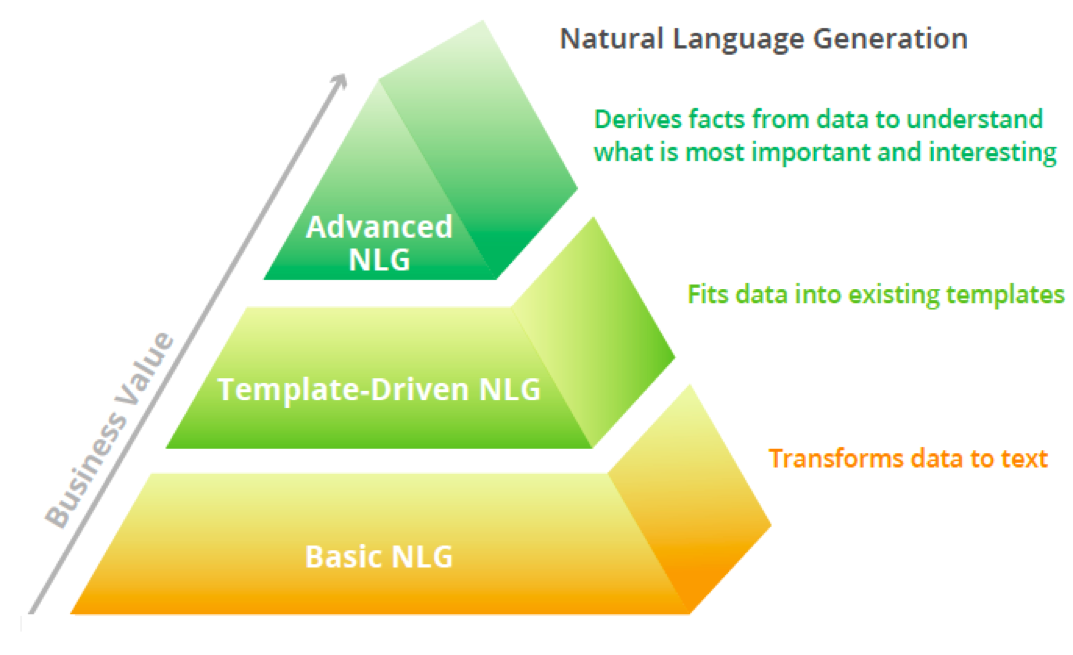
\includegraphics[width=0.46\textwidth,
                   height=0.32\textheight,
                   keepaspectratio]{images/nlg.png}
  \caption{\textit{Natural Language Generation}}
  \label{fig:nlg}
\end{figure}

Bagian ini membahas pendekatan pembangkitan bahasa alami berbasis templat untuk menghasilkan variasi respons dari data internal perusahaan. Pembahasan mencakup konsep NLG berbasis templat, keamanan data dalam implementasi NLG internal, dan evaluasi kualitas teks yang dihasilkan. Pendekatan ini memastikan bahwa respons yang dihasilkan bervariasi dan natural sembari tetap menjaga keamanan dan privasi data perusahaan.

\subsection{Konsep \textit{Natural Language Generation}}

\textit{Natural Language Generation} (NLG) (lihat ilustrasi pada Gambar~\ref{fig:nlg}) adalah proses menghasilkan teks bahasa alami dari representasi data terstruktur. Dalam konteks \textit{chatbot} Business Intelligence, NLG digunakan untuk mengubah hasil kueri basis data menjadi respons bahasa natural yang mudah dipahami pengguna \autocite{kale2020template}. NLG memungkinkan sistem untuk menyajikan informasi numerik dan data terstruktur dalam format naratif yang lebih mudah dicerna.

Pasar NLP global diproyeksikan tumbuh dari USD 35,43 miliar pada tahun 2024 menjadi USD 438,08 miliar pada tahun 2034, dengan CAGR sebesar 28,6\% \autocite{Precedence2025}. Pertumbuhan eksponensial ini didorong oleh meningkatnya adopsi teknologi AI, \textit{cloud computing}, dan kebutuhan akan analisis data tidak terstruktur di berbagai sektor industri. Pertumbuhan pasar ini menunjukkan relevansi dan urgensi pengembangan sistem NLG untuk mendukung kebutuhan bisnis modern.

\subsection{\textit{Template-Based Natural Language Generation}}

Sistem NLG berbasis templat memetakan \textit{input} non-linguistik secara langsung ke struktur linguistik yang berisi "celah" atau \textit{placeholders} yang diisi selama \textit{output}. Pendekatan ini menggunakan templat yang telah ditentukan sebelumnya dengan slot yang dapat diisi dengan data aktual dari hasil kueri basis data.

Contoh implementasi templat sederhana mencakup struktur seperti "Penjualan pada \texttt{[bulan]} mencapai \texttt{[nilai]}, meningkat \texttt{[persentase]}\% dari bulan sebelumnya." Sistem kemudian mengisi placeholder dengan data aktual: "Penjualan pada Oktober 2025 mencapai Rp 5,2 miliar, meningkat 15\% dari bulan sebelumnya." \autocite{kale2020template}.

Keuntungan utama pendekatan berbasis templat adalah kontrol penuh atas output, kecepatan generasi yang tinggi, tidak memerlukan \textit{dataset} pelatihan besar, dan kemudahan maintenance dan modifikasi. Sistem dapat menghasilkan variasi output dengan mendefinisikan multiple templat untuk skenario yang sama, menghindari respons yang monoton \autocite{kapoor2023implementing}.

\subsection{\textit{Template Rewriting} dengan \textit{Pre-trained Language Models}}

Pendekatan lanjutan dalam NLG berbasis templat melibatkan penggunaan model bahasa pre-trained untuk menulis ulang templat sederhana menjadi teks yang lebih koheren dan natural. Metode ini menggabungkan keuntungan templat dengan fleksibilitas model bahasa neural \autocite{kale2020template,rebuffel2020fewshot}.

Arsitektur sistem mencakup tiga tahapan utama. Tahap pertama adalah modul kebijakan menghasilkan sekumpulan tindakan berdasarkan konteks. Tahap kedua adalah templat sederhana mengkonversi setiap tindakan menjadi \textit{utterance} bahasa alami. Tahap ketiga adalah model \textit{encoder-decoder} seperti T5 menulis ulang gabungan \textit{utterances} menjadi respons percakapan yang koheren \autocite{kale2020template}.

Pendekatan ini memungkinkan sistem untuk menghasilkan respons yang secara semantik benar dari templat, kemudian model bahasa memperbaiki koherensi dan kealamian teks. Metode \textit{template rewriting} telah menunjukkan peningkatan sample efficiency yang signifikan dibandingkan metode end-to-end, dengan jumlah templat yang tumbuh linear terhadap jumlah slot dibandingkan pertumbuhan kombinatorial \autocite{rebuffel2020fewshot}.

\subsection{Keamanan dan Privasi Data dalam NLG Internal}

Implementasi NLG dalam lingkungan perusahaan memerlukan pertimbangan keamanan yang ketat untuk melindungi data sensitif dan mencegah kebocoran informasi. Sistem NLG internal harus dirancang dengan prinsip \textit{privacy-by-design} untuk memastikan data perusahaan tetap aman.

\subsubsection{\textit{Differential Privacy} untuk NLG}

\textit{Differential Privacy} (DP) adalah kerangka kerja yang memberikan jaminan privasi secara matematis, memastikan bahwa kontribusi individu dalam \textit{dataset} dibatasi \autocite{feyisetan2022differential,mireshghallah2022differentially}. Dalam konteks NLG, DP dapat diterapkan melalui dua pendekatan utama. Pendekatan pertama adalah pelatihan model dengan DP-SGD yang menambahkan noise pada gradien selama pelatihan. Pendekatan kedua adalah perturbasi representasi teks yang menambahkan noise pada \textit{embedding} sebelum generasi.

Parameter privasi $\epsilon$\label{sym:epsilon} mengontrol tingkat privasi yang diberikan, dengan nilai $\epsilon$ yang lebih kecil memberikan privasi yang lebih kuat tetapi dapat mengurangi utility model. Implementasi DP dalam NLG memerlukan trade-off yang cermat antara privasi dan kualitas output \autocite{luo2024data}.

\subsubsection{Strategi Keamanan Data dalam NLG}

Implementasi NLG internal yang aman memerlukan beberapa strategi keamanan berlapis \autocite{itconvergence2024generative}. Strategi pertama adalah enkripsi data dengan mengenkripsi data saat transit menggunakan TLS/SSL dan saat istirahat untuk melindungi data sensitif. Strategi kedua adalah kontrol akses yang ketat dengan menerapkan autentikasi dan otorisasi yang robust, menggunakan prinsip \textit{least privilege}. Strategi ketiga adalah data minimization dengan hanya menggunakan data minimum yang diperlukan untuk generasi respons. Strategi keempat adalah \textit{template-based approach} yang membatasi generasi hanya pada templat yang telah diverifikasi, mencegah generasi teks bebas yang dapat membocorkan informasi sensitif.

Strategi kelima adalah audit dan monitoring dengan mencatat semua aktivitas NLG untuk deteksi anomali dan audit keamanan. Strategi terakhir adalah \textit{secure deployment environment} dengan mengamankan infrastruktur server, firewall, dan menjaga software tetap terbarukan \autocite{itconvergence2024generative,aws2024securing}.

\subsubsection{Mitigasi Risiko dalam NLG Internal}

Risiko utama dalam implementasi NLG internal mencakup kebocoran data sensitif melalui output yang dihasilkan, \textit{prompt injection} yang dapat memanipulasi model untuk menghasilkan output tidak diinginkan, dan \textit{data tampering} yang dapat menyebabkan respons AI yang salah. Mitigasi risiko ini memerlukan pendekatan multi-layer \autocite{postgresql2024generative}.

Teknik mitigasi mencakup pemfilteran output untuk memeriksa dan menyensor informasi sensitif sebelum ditampilkan ke pengguna. \textit{Input validation} digunakan untuk memvalidasi semua \textit{input} dan menolak pola yang mencurigakan. \textit{Template whitelisting} membatasi generasi hanya pada templat yang telah disetujui. Implementasi \textit{role-based access control} (RBAC) memastikan pengguna hanya dapat mengakses data sesuai peran mereka. Regular security assessment dilakukan untuk menguji kerentanan sistem secara berkala \autocite{edpb2025privacy,velotix2025security}.

\subsection{Evaluasi Kualitas \textit{Natural Language Generation}}

Evaluasi kualitas keluaran \textit{Natural Language Generation} (NLG) merupakan aspek penting untuk memastikan bahwa teks yang dihasilkan tidak hanya benar secara faktual, tetapi juga mudah dipahami, wajar, dan bermanfaat bagi pengguna. Dalam konteks penelitian ini, fungsi utama modul NLG adalah menyajikan hasil analisis dan prediksi dalam bentuk jawaban yang lebih ramah pengguna sehingga penilaian kualitas dari sudut pandang pengguna menjadi sangat sentral. Meskipun demikian, sejumlah penelitian terdahulu menunjukkan bahwa kombinasi antara metrik evaluasi otomatis dan penilaian manusia (subjektif) memberikan gambaran yang lebih komprehensif mengenai kualitas keluaran NLG \autocite{Celikyilmaz2020EvalTextGen,Sai2020NLGSurvey,vanDerLee2021HumanEval}.

\subsubsection{Metrik Otomatis untuk Evaluasi NLG}

Berbagai survei mengenai evaluasi NLG mengelompokkan metrik otomatis ke dalam beberapa kategori utama, seperti metrik berbasis kecocokan permukaan (\textit{string-matching}), metrik berbasis pemetaan vektor (\textit{embedding-based}), dan metrik berbasis model pembelajaran mesin \autocite{Celikyilmaz2020EvalTextGen,Sai2020NLGSurvey,Gao2024LLMNLG}.

Kategori pertama adalah metrik berbasis referensi yang membandingkan keluaran sistem dengan satu atau beberapa teks rujukan yang ditulis manusia. Contoh yang paling banyak digunakan adalah BLEU\label{abbr:BLEU} (\textit{Bilingual Evaluation Understudy}) yang mengukur kecocokan \textit{n-gram} antara keluaran dan teks rujukan, dengan rumus umum \autocite{Sai2020NLGSurvey}:
\[
\text{BLEU (\textit{Bilingual Evaluation Understudy})} = BP \times \exp\left(\sum_{n=1}^{N} w_n \log p_n\right)
\]
dengan \(p_n\) menyatakan presisi \textit{n-gram} dan \(BP\) adalah faktor penalti panjang (\textit{brevity penalty}). Metrik lain seperti METEOR (\textit{Metric for Evaluation of Translation with Explicit ORdering}) memasukkan faktor sinonim dan \textit{stemming}, sedangkan ROUGE\label{abbr:ROUGE} (\textit{Recall-Oriented Understudy for Gisting Evaluation}) berfokus pada daya ingat (\textit{recall}) dan banyak digunakan untuk evaluasi peringkasan teks \autocite{Celikyilmaz2020EvalTextGen,Sai2020NLGSurvey}.

Kategori kedua adalah metrik berbasis penyajian vektor (\textit{embedding-based}), yang menggunakan representasi neural untuk mengukur kesamaan semantik, bukan hanya kesamaan permukaan. Contohnya adalah BERTScore yang memanfaatkan \textit{embedding} BERT untuk menghitung kesamaan kontekstual antara token keluaran dan token rujukan. Metrik ini umumnya menunjukkan korelasi yang lebih baik dengan penilaian manusia dibandingkan metrik \textit{string-matching} murni, terutama ketika terdapat banyak cara wajar untuk mengekspresikan makna yang sama \autocite{Celikyilmaz2020EvalTextGen,Gao2024LLMNLG}.

Meskipun berguna untuk perbandingan model secara cepat dan konsisten, berbagai studi meta-evaluasi menegaskan bahwa metrik otomatis ini hanya menangkap sebagian aspek kualitas dan sering kali berkorelasi sedang atau bahkan rendah dengan penilaian manusia, terutama pada tugas dialog dan percakapan yang bersifat terbuka \autocite{Celikyilmaz2020EvalTextGen,Sai2020NLGSurvey,Xiao2023MetricEval}. Oleh karena itu, metrik otomatis umumnya direkomendasikan sebagai pelengkap, bukan pengganti, evaluasi subjektif oleh manusia.

\subsubsection{Evaluasi Subjektif Berbasis Pengguna}

Sejumlah survei dan studi empiris menegaskan bahwa evaluasi manusia tetap dianggap sebagai standar emas (\textit{gold standard}) dalam penilaian kualitas keluaran NLG, khususnya untuk aspek yang bersifat kualitatif seperti kewajaran bahasa, keterpahaman, dan kegunaan bagi pengguna akhir \autocite{vanDerLee2021HumanEval,Celikyilmaz2020EvalTextGen,Morrison2021ReproSubjective}. Evaluasi subjektif ini umumnya dilakukan dengan meminta penilai manusia memberikan skor pada skala Likert (biasanya 1--5 atau 1--7) terhadap beberapa dimensi kualitas teks.

Praktik evaluasi manusia yang umum pada sistem NLG dan sejumlah dimensi yang sering digunakan, antara lain \autocite{vanDerLee2021HumanEval}:
\begin{enumerate}[label=\alph*.]
    \item \textbf{Kewajaran/\textit{Naturalness}}: Sejauh mana teks terdengar wajar seperti ditulis penutur asli dan tidak tampak kaku atau \textit{robotik}.
    \item \textbf{Kelancaran/\textit{Fluency}}: Sejauh mana teks bebas dari kesalahan tata bahasa dan struktur kalimat yang janggal.
    \item \textbf{Kecukupan/\textit{Adequacy} atau \textit{Informativeness}}: Sejauh mana teks menyampaikan informasi yang tepat dan memadai terkait masukan.
    \item \textbf{Koherensi/\textit{Coherence}}: Sejauh mana kalimat-kalimat dalam teks saling tersambung secara logis dan membentuk alur yang mudah diikuti.
\end{enumerate}

Kerangka evaluasi seperti ConSiDERS dan panduan evaluasi subjektif yang dapat direproduksi menekankan pentingnya perancangan instruksi penilaian yang jelas, pemilihan skala yang konsisten, dan penggunaan beberapa penilai untuk meningkatkan reliabilitas \autocite{Elangovan2023ConSiDERS,Morrison2021ReproSubjective}. Dalam surveinya juga digarisbawahi bahwa untuk banyak tugas NLG, korelasi antara metrik otomatis dan penilaian manusia tidak cukup tinggi sehingga penilaian manusia tetap diperlukan, terutama ketika tujuan utama sistem adalah meningkatkan mutu pengalaman pengguna, bukan mengoptimalkan skor metrik otomatis tertentu \autocite{Sai2020NLGSurvey}.

Dalam konteks \textit{chatbot} berbasis AI, sejumlah penelitian di bidang kualitas layanan dan pengalaman pengguna mengaitkan kualitas percakapan alami dengan dimensi seperti \textit{friendliness}, \textit{usefulness}, kejelasan jawaban, serta persepsi kemudahan penggunaan. Studi tentang kualitas layanan AI-\textit{chatbot} menunjukkan bahwa kemampuan percakapan yang wajar, relevansi informasi, dan kecepatan respons berkontribusi signifikan terhadap kepuasan, kepercayaan, dan niat pengguna untuk terus menggunakan layanan tersebut \autocite{Syarifudin2024AIChatbotQuality,hsu2023chatbotsatisfaction}. Hal ini sejalan dengan fokus penelitian ini, dengan fungsi utama modul NLG adalah membuat jawaban sistem lebih ramah pengguna dan mudah dipahami, bukan menghasilkan variasi bahasa yang kreatif tanpa batas.

Dengan demikian, evaluasi subjektif dalam konteks \textit{chatbot} BI dapat difokuskan pada beberapa dimensi utama berikut.
\begin{enumerate}[label=\alph*.]
    \item \textbf{Kewajaran Bahasa}: Apakah jawaban terdengar alami dan tidak kaku.
    \item \textbf{Kejelasan dan Keterpahaman}: Apakah isi jawaban mudah dipahami oleh pengguna nonteknis.
    \item \textbf{Kegunaan/\textit{Usefulness}}: Apakah jawaban benar-benar membantu pengguna menjawab pertanyaan bisnis yang diajukan.
    \item \textbf{Kenyamanan Interaksi}: Sejauh mana gaya bahasa dan struktur jawaban mendukung pengalaman percakapan yang menyenangkan.
\end{enumerate}

Dimensi-dimensi tersebut dapat diukur menggunakan skala Likert oleh sejumlah penilai internal pada tahap pengujian sistem, mengikuti praktik yang direkomendasikan dalam literatur evaluasi NLG dan kualitas \textit{chatbot} \autocite{vanDerLee2021HumanEval,Syarifudin2024AIChatbotQuality}.

\subsubsection{Kriteria Performa NLG dalam Literatur}

Survei-survei terkini mengenai evaluasi NLG menekankan bahwa tidak ada satu nilai ambang (\textit{threshold}) numerik yang bersifat universal untuk menyatakan bahwa suatu sistem ``cukup baik'' karena nilai metrik sangat bergantung pada tugas, data, dan desain sistem yang dievaluasi \autocite{Celikyilmaz2020EvalTextGen,Sai2020NLGSurvey,Gao2024LLMNLG}. Oleh karena itu, karya-karya ilmiah umumnya:
\begin{enumerate}[label=\alph*.]
    \item Membandingkan metrik otomatis (seperti BLEU, ROUGE, BERTScore) relatif terhadap model dasar atau pendekatan lain pada tugas yang sama, dan
    \item Menggunakan penilaian manusia sebagai landasan utama, dengan rata-rata skor pada skala 1--5 atau 1--7 untuk dimensi seperti kewajaran, kelancaran, dan kecukupan, dengan skor rata-rata yang mendekati ujung atas skala lazim dipandang sebagai indikasi kualitas tinggi \autocite{vanDerLee2021HumanEval,Celikyilmaz2020EvalTextGen}.
\end{enumerate}

Dalam studi-studi dialog dan percakapan, sistem yang dianggap berkualitas baik biasanya menunjukkan:
\begin{enumerate}[label=\alph*.]
    \item Peningkatan signifikan pada metrik otomatis dibandingkan model dasar, \textit{namun} penulis tetap menekankan bahwa korelasi metrik otomatis dengan penilaian manusia terbatas dan konteks spesifik harus diperhatikan \autocite{Sai2020NLGSurvey,Xiao2023MetricEval},
    \item Rata-rata skor penilaian manusia yang tinggi untuk dimensi kewajaran, kelancaran, dan relevansi, serta
    \item Indikator kepuasan dan persepsi kualitas layanan yang positif pada studi pengguna, seperti peningkatan kepercayaan, kenyamanan interaksi, dan niat untuk terus menggunakan \textit{chatbot} \autocite{Syarifudin2024AIChatbotQuality,hsu2023chatbotsatisfaction}.
\end{enumerate}

Berdasarkan informasi tersebut, literatur menyarankan bahwa pemilihan metrik evaluasi NLG hendaknya disesuaikan dengan tujuan sistem. Dalam sistem \textit{Business Intelligence} berbasis \textit{chatbot} yang memanfaatkan NLG terutama untuk menjadikan jawaban lebih ramah pengguna dan mudah dipahami, metrik subjektif yang berfokus pada persepsi pengguna (kewajaran, keterpahaman, kegunaan) dapat dipandang sebagai indikator utama, sedangkan metrik otomatis seperti BLEU atau BERTScore dapat digunakan secara opsional untuk memantau konsistensi bentuk bahasa sepanjang pengembangan \autocite{Celikyilmaz2020EvalTextGen,vanDerLee2021HumanEval}.

% ==============================================================================
\section{\textit{Time Series Forecasting}}
% ==============================================================================
\begin{figure}[t]
  \centering
  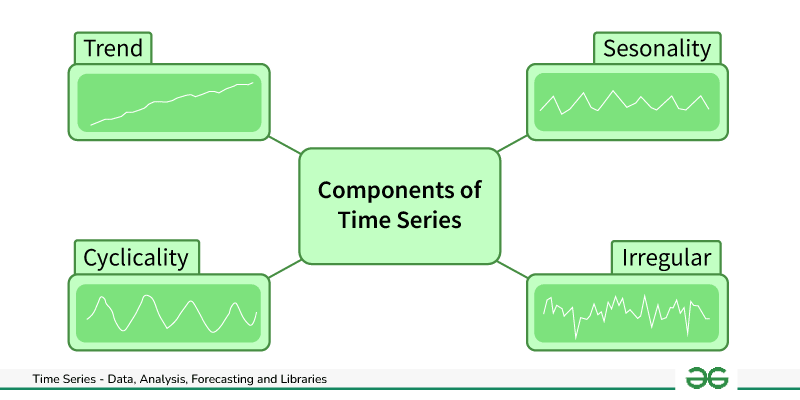
\includegraphics[width=0.46\textwidth,
                   height=0.32\textheight,
                   keepaspectratio]{images/timeseries.png}
  \caption{\textit{Time Series Forecasting}}
  \label{fig:tsf}
\end{figure}

Peramalan deret waktu (\textit{Time Series Forecasting}) (diilustrasikan pada Gambar~\ref{fig:tsf}) adalah proses memprediksi nilai masa depan dari suatu variabel berdasarkan observasi nilai-nilai masa lalu dari variabel yang sama secara berurutan waktu. Dalam domain bisnis, metodologi ini fundamental untuk memproyeksikan metrik utama, seperti volume penjualan, permintaan layanan pelanggan, atau tingkat retensi pengguna, sehingga memungkinkan organisasi mengambil langkah antisipatif dan menyusun strategi berbasis data.

Bagian ini membahas konsep peramalan deret waktu, model-model statistik dan pembelajaran mendalam yang digunakan, serta evaluasi performa yang komprehensif. Pembahasan mencakup ARIMA, SARIMA\label{abbr:SARIMA}, LSTM, serta perbandingan karakteristik dan performa masing-masing metode. Pemahaman yang mendalam tentang berbagai pendekatan peramalan ini menjadi fondasi penting dalam memilih dan mengimplementasikan model yang sesuai dengan karakteristik data dan kebutuhan aplikasi.

\subsection{Konsep \textit{Time Series} dan Peramalan}

\textit{Time series} adalah serangkaian titik data yang diindeks dalam urutan waktu, dan peramalan deret waktu adalah proses menggunakan model untuk memprediksi nilai masa depan berdasarkan nilai yang diamati sebelumnya. Peramalan akurat sangat penting untuk perencanaan strategis dan pengambilan keputusan di berbagai domain bisnis.

Pasar \textit{time series forecasting} global mencapai USD 9,62 miliar pada tahun 2023 dan diperkirakan tumbuh menjadi USD 36,9 miliar pada tahun 2032 dengan CAGR sebesar 16,12\% \autocite{WiseGuyReports2024}. Pertumbuhan ini menunjukkan meningkatnya adopsi teknik peramalan deret waktu di berbagai industri untuk mendukung pengambilan keputusan berbasis data, termasuk peramalan permintaan layanan pelanggan, prediksi penjualan, dan analisis tren bisnis. Proyeksi pertumbuhan pasar ini mengindikasikan relevansi dan urgensi pengembangan sistem peramalan yang akurat dan dapat diandalkan.

\subsection{Model Peramalan Statistik Klasik sebagai \textit{Baseline}}
\label{subsec:model-statistik}

Sebelum membahas model berbasis pembelajaran mendalam, penting untuk memahami model statistik klasik yang digunakan sebagai \textit{baseline} dalam penelitian ini. Model statistik seperti ARIMA dan Prophet merupakan tolok ukur yang lazim digunakan dalam evaluasi peramalan deret waktu karena sifatnya yang dapat diinterpretasikan, tidak memerlukan data dalam jumlah sangat besar, dan relatif cepat untuk dilatih. Perbandingan terhadap \textit{baseline} statistik ini memungkinkan penilaian yang objektif mengenai apakah model \textit{deep learning} yang lebih kompleks benar-benar memberikan keunggulan yang sepadan dengan biaya komputasi yang lebih tinggi.

\subsubsection{ARIMA dan SARIMA}

ARIMA (\textit{Autoregressive Integrated Moving Average}) adalah model peramalan deret waktu statistik yang menggabungkan tiga komponen utama: komponen autoregresif (AR) yang memodelkan pengaruh nilai masa lalu terhadap nilai saat ini, komponen diferensiasi (I) yang mengubah deret waktu menjadi stasioner melalui operasi selisih, dan komponen rata-rata bergerak (MA) yang memodelkan pengaruh kesalahan masa lalu. Model ARIMA dinotasikan sebagai ARIMA(\(p, d, q\))\label{sym:pdq} di mana \(p\) adalah orde autoregresif, \(d\) adalah derajat diferensiasi, dan \(q\) adalah orde rata-rata bergerak \autocite{Petropoulos2022ForecastingPractice,Spiliotis2020ForecastingBenchmarks}.

Untuk data yang mengandung pola musiman, digunakan model SARIMA (\textit{Seasonal ARIMA}) yang dinotasikan sebagai SARIMA(\(p, d, q\))(\(P, D, Q\))\label{sym:PDQ}\(m\)\label{sym:m} di mana \(P\), \(D\), \(Q\) adalah parameter musiman dan \(m\) adalah periode musiman (misalnya \(m = 12\) untuk data bulanan). SARIMA mampu menangkap pola musiman berulang yang lazim ditemukan pada data bisnis seperti penjualan dan \textit{churn} pelanggan \autocite{Petropoulos2022ForecastingPractice}.

Keunggulan utama ARIMA dan SARIMA terletak pada interpretabilitas tinggi, kebutuhan data yang relatif sedikit, dan efisiensi komputasi. Namun, model ini mengasumsikan linearitas dalam hubungan temporal dan memerlukan pemilihan parameter (\(p, d, q\)) yang cermat melalui analisis fungsi autokorelasi (ACF) dan autokorelasi parsial (PACF) \autocite{Petropoulos2022ForecastingPractice,Spiliotis2020ForecastingBenchmarks}.

\subsubsection{Prophet}

Prophet adalah model peramalan deret waktu yang dikembangkan oleh Meta (Facebook) dan dirancang untuk bekerja dengan baik pada data bisnis yang memiliki tren kuat, efek musiman yang jelas, dan \textit{outlier} yang umum \autocite{Tuncer2023ARIMAProphetLSTM,Masini2023MLTimeSeriesForecasting}. Prophet menggunakan pendekatan dekomposisi aditif yang memisahkan deret waktu menjadi komponen tren \(T(t)\)\label{sym:Tt}\label{sym:t}, musiman \(S(t)\)\label{sym:St}, efek hari raya \(H(t)\)\label{sym:Ht}, dan kesalahan residual \(\epsilon_t\):

\begin{equation}
y(t) = T(t) + S(t) + H(t) + \epsilon_t
\end{equation}
\eqcaption{Dekomposisi Aditif Deret Waktu (\textit{Prophet})}

Komponen tren dimodelkan menggunakan fungsi pertumbuhan linier atau logistik yang dapat menangkap titik perubahan (\textit{changepoints}) secara otomatis. Komponen musiman dimodelkan menggunakan deret Fourier untuk menangkap pola musiman harian, mingguan, dan tahunan secara fleksibel.

Keunggulan Prophet adalah kemudahan penggunaan, kemampuan menangani nilai hilang (\textit{missing values}) dan \textit{outlier} secara otomatis, serta dukungan untuk variabel regresor eksternal. Namun, Prophet cenderung kurang optimal untuk pola temporal yang sangat kompleks dan non-linear jika dibandingkan dengan model \textit{deep learning} \autocite{Tuncer2023ARIMAProphetLSTM,Masini2023MLTimeSeriesForecasting}.

\subsubsection{Keterbatasan Model Statistik dan Motivasi Penggunaan \textit{Deep Learning}}

Meskipun model statistik seperti ARIMA dan Prophet unggul dalam hal interpretabilitas dan efisiensi komputasi, terdapat sejumlah keterbatasan yang memotivasi penggunaan model \textit{deep learning} dalam penelitian ini. Pertama, ARIMA dan SARIMA mengasumsikan linearitas sehingga kurang mampu menangkap hubungan temporal yang kompleks dan non-linear yang umum dalam data bisnis \autocite{Petropoulos2022ForecastingPractice,Spiliotis2020ForecastingBenchmarks}. Kedua, model statistik univariat seperti ARIMA tidak secara langsung memanfaatkan informasi dari variabel-variabel lain yang berkorelasi, sehingga kurang optimal untuk data multivariat \autocite{Masini2023MLTimeSeriesForecasting}. Ketiga, studi empiris pada data \textit{e-commerce} dan telekomunikasi menunjukkan bahwa model LSTM dan GRU konsisten mengungguli ARIMA dengan pengurangan \textit{error} sekitar 12--18\% pada data dengan pola musiman dan ketergantungan temporal yang kompleks \autocite{Sunendar2025ComparisonARIMALSTMGRU,Tuncer2023ARIMAProphetLSTM}.

Dengan demikian, pendekatan dalam penelitian ini adalah menggunakan ARIMA dan Prophet sebagai \textit{baseline} yang terukur, kemudian membandingkannya dengan model \textit{deep learning} (LSTM dan GRU) untuk memvalidasi bahwa kompleksitas tambahan dari model \textit{deep learning} benar-benar memberikan peningkatan akurasi yang signifikan dalam konteks data indikator bisnis yang digunakan.

\subsection{Model Peramalan Deret Waktu Berbasis \textit{Deep Learning}}

Sistem peramalan dalam penelitian ini memanfaatkan pendekatan berbasis pembelajaran mendalam (\textit{deep learning}) yang dirancang khusus untuk menangani data deret waktu multivariat (\textit{multivariate time series}) dengan pola temporal yang kompleks. Sistem mengimplementasikan dua arsitektur utama, yaitu LSTM dan GRU, untuk memaksimalkan akurasi prediksi terhadap indikator kinerja bisnis seperti volume pesanan, tingkat \textit{churn} pelanggan, dan proyeksi pendapatan \autocite{Yunita2025NNComparison,Zhang2024ComprehensiveTSFSurvey}. Arsitektur \textit{Temporal Fusion Transformer} (TFT) dikaji sebagai referensi teoretis namun tidak diimplementasikan pada purwarupa ini (lihat Subbab~\ref{subsec:tft-literatur}).

\subsubsection{LSTM (\textit{Long Short-Term Memory}) untuk Peramalan Deret Waktu}

LSTM adalah jenis jaringan saraf berulang (\textit{Recurrent Neural Network}, RNN)\label{abbr:RNN} yang dirancang untuk mengatasi masalah gradien menghilang (\textit{vanishing gradient}) pada RNN tradisional dan mampu mempelajari dependensi jangka panjang dalam data sekuens \autocite{Yunita2025NNComparison}. Arsitektur LSTM terdiri dari sel memori dan tiga gerbang utama: gerbang lupa (\textit{forget gate}) yang menentukan informasi apa dari sel memori yang harus dibuang, gerbang masukan (\textit{input gate}) yang menentukan informasi baru apa yang akan disimpan, dan gerbang keluaran (\textit{output gate}) yang menentukan bagian mana dari sel memori yang akan menjadi keluaran.

Persamaan matematis LSTM dapat ditulis sebagai berikut \autocite{Yunita2025NNComparison}:
\phantomsection\label{sym:ft}\label{sym:sigmoid}\label{sym:it}\label{sym:tanh}\label{sym:xt}\label{sym:ct}\label{sym:ot}\label{sym:ht}
\begin{align}
f_t &= \sigma(W_f \cdot [h_{t-1}, x_t] + b_f) \\
i_t &= \sigma(W_i \cdot [h_{t-1}, x_t] + b_i) \\
\tilde{C}_t &= \tanh(W_C \cdot [h_{t-1}, x_t] + b_C) \\
C_t &= f_t * C_{t-1} + i_t * \tilde{C}_t \\
o_t &= \sigma(W_o \cdot [h_{t-1}, x_t] + b_o) \\
h_t &= o_t * \tanh(C_t)
\end{align}
\eqcaption{Persamaan Gerbang LSTM}

Dalam persamaan ini, \(f_t\) adalah gerbang lupa, \(i_t\) adalah gerbang masukan, \(o_t\) adalah gerbang keluaran, \(C_t\) adalah keadaan sel (\textit{cell state}), \(h_t\) adalah keadaan tersembunyi (\textit{hidden state}), \(\sigma\) adalah fungsi sigmoid, serta \(W\)\label{sym:W} dan \(b\)\label{sym:b} adalah matriks bobot dan vektor bias yang dipelajari selama pelatihan.

LSTM unggul dalam menangani data deret waktu yang kompleks dengan dependensi jangka panjang dan pola non-linear. Kemampuan model untuk mengingat informasi relevan dari masa lalu yang jauh menjadikannya sangat efektif untuk aplikasi seperti peramalan permintaan atau tingkat \textit{churn} pelanggan yang dipengaruhi oleh berbagai faktor temporal yang kompleks \autocite{Yunita2025NNComparison}.

\subsubsection{GRU (\textit{Gated Recurrent Unit}) sebagai Alternatif LSTM}

GRU adalah varian yang lebih sederhana dari LSTM, menawarkan performa yang sebanding dengan menggunakan arsitektur yang lebih ringkas dan parameter yang lebih sedikit \autocite{Yunita2025NNComparison,Zhang2024ComprehensiveTSFSurvey}. GRU memiliki dua gerbang utama: gerbang reset (\textit{reset gate}) dan gerbang pembaruan (\textit{update gate}), menggabungkan fungsi gerbang lupa dan gerbang masukan LSTM menjadi satu gerbang pembaruan.

Persamaan matematis GRU dapat ditulis sebagai \autocite{Yunita2025NNComparison}:
\phantomsection\label{sym:rt}\label{sym:zt}
\begin{align}
r_t &= \sigma(W_r \cdot [h_{t-1}, x_t] + b_r) \\
z_t &= \sigma(W_z \cdot [h_{t-1}, x_t] + b_z) \\
\tilde{h}_t &= \tanh(W \cdot [r_t * h_{t-1}, x_t] + b) \\
h_t &= (1 - z_t) * h_{t-1} + z_t * \tilde{h}_t
\end{align}
\eqcaption{Persamaan Gerbang GRU}

Dalam persamaan ini, \(r_t\) adalah gerbang reset, \(z_t\) adalah gerbang pembaruan, dan \(\tilde{h}_t\) adalah calon keadaan tersembunyi. Studi empiris menunjukkan bahwa GRU sering memberikan hasil yang setara atau bahkan lebih baik daripada LSTM pada berbagai tugas peramalan deret waktu, dengan keuntungan pelatihan yang lebih cepat dan kebutuhan komputasi yang lebih rendah \autocite{Yunita2025NNComparison,Jeaab2024LSTMGRUXGBoost}.

\subsubsection{\textit{Temporal Fusion Transformer} (TFT) untuk Data Multivariat}
\label{subsec:tft-literatur}
\label{subsec:tft-literatur}

\textit{Temporal Fusion Transformer} (TFT) adalah arsitektur berbasis perhatian (\textit{attention-based}) yang dirancang khusus untuk peramalan deret waktu multi-horizon pada data multivariat yang kompleks \autocite{Lim2021TFT,Zhang2024ComprehensiveTSFSurvey}. TFT menggabungkan kekuatan mekanisme perhatian diri (\textit{self-attention}) Transformer dengan lapisan berulang untuk pemrosesan lokal, memungkinkan model menangkap ketergantungan temporal pada berbagai skala waktu.

Arsitektur TFT terdiri dari beberapa komponen utama \autocite{Lim2021TFT,Hartanto2024TFTEnhanced}:
\begin{enumerate}[label=\alph*.]
    \item \textbf{Variabel \textit{Input} Tipe-Campuran}: TFT menangani masukan eksogen tergantung waktu (\textit{time-dependent exogenous features}) yang terdiri dari masukan yang tidak diketahui sebelumnya dan masukan yang diketahui, serta kovariat statis yang memberikan konteks tentang entitas yang diukur.
    
    \item \textbf{Jaringan Pemilihan Variabel (\textit{Variable Selection Network})}: Komponen ini secara adaptif memilih fitur yang paling relevan dari antara semua masukan, meningkatkan interpretabilitas dan mengurangi kebisingan dari fitur yang tidak relevan \autocite{Lim2021TFT}.
    
    \item \textbf{Lapisan Gerbang Residu (\textit{Gated Residual Networks})}: Lapisan ini menerapkan mekanisme gerbang untuk menekan komponen yang tidak perlu, meningkatkan kemampuan model untuk fokus pada pola penting \autocite{Lim2021TFT}.
    
    \item \textbf{Mekanisme \textit{Multi-Head Attention}}: Mekanisme perhatian diri memungkinkan model menangkap hubungan jangka panjang dan pola kompleks dalam data, memberikan ketepatan prediksi yang tinggi pada berbagai horizon waktu \autocite{Hartanto2024TFTEnhanced}.
\end{enumerate}

Berbeda dengan RNN yang memproses data secara sekuensial, TFT dapat memproses seluruh urutan masukan secara paralel, menghasilkan pelatihan yang lebih cepat. Penelitian menunjukkan bahwa TFT unggul dalam menangani skenario peramalan multivariat yang kompleks dengan banyak fitur yang saling berinteraksi, seperti kasus prediksi kinerja bisnis yang melibatkan banyak indikator yang saling terkait \autocite{Hartanto2024TFTEnhanced,Cheng2025MultivariateTFFEng}.

\subsubsection{Model Hibrida dan \textit{Ensemble}}

Penelitian terkini menunjukkan bahwa kombinasi hibrida dari arsitektur yang berbeda sering memberikan hasil yang lebih baik daripada model tunggal karena setiap arsitektur menangkap aspek berbeda dari pola temporal dalam data \autocite{Yunita2025NNComparison,Zhang2024ComprehensiveTSFSurvey}.

Model hibrida \textbf{GRU-LSTM} menggabungkan keunggulan komplementer dari kedua arsitektur berulang. Studi pada prediksi suhu harian menunjukkan bahwa model hibrida GRU-LSTM mencapai RMSE sebesar 0{,}07499 dan MAE sebesar 0{,}0578 pada skenario masukan 15 hari, dengan \(R^2\) mendekati 1 (0{,}9937), menunjukkan performa yang sangat baik \autocite{Diqi2023GRULSTMHybrid}. Keuntungan pendekatan hibrida terletak pada fleksibilitas untuk memanfaatkan kapabilitas pemrosesan lokal GRU yang efisien sekaligus pembelajaran dependensi jangka panjang yang kuat dari LSTM.

Pendekatan ensemble yang menggabungkan keluaran dari multiple model (misalnya LSTM, GRU, dan TFT) juga terbukti meningkatkan robustness dan ketepatan prediksi, terutama dalam menangani variabilitas dan ketidakpastian dalam data bisnis real-world \autocite{Zhang2024ComprehensiveTSFSurvey,Yunita2025NNComparison}.

\subsubsection{Perbandingan Karakteristik Model Peramalan \textit{Deep Learning}}

Berbagai penelitian empiris telah membandingkan kinerja LSTM, GRU, dan TFT pada berbagai skenario peramalan deret waktu. Tabel~\ref{tab:dl-forecasting-comparison} menyajikan perbandingan karakteristik utama dari ketiga arsitektur berdasarkan sintesis dari penelitian-penelitian terdahulu.

\begin{longtable}{|p{1.8cm}|p{3.5cm}|p{3.8cm}|p{3cm}|}
\caption{Perbandingan Karakteristik Model Peramalan Deret Waktu}
\label{tab:dl-forecasting-comparison}\\
\hline
\textbf{Metode} & \textbf{Kelebihan} & \textbf{Kekurangan} & \textbf{Karakteristik} \tabularnewline
\hline
\endfirsthead

\multicolumn{4}{c}%
{\tablename\ \thetable\ -- {Perbandingan Model Peramalan Deret Waktu (lanjutan)}} \\
\hline
\textbf{Metode} & \textbf{Kelebihan} & \textbf{Kekurangan} & \textbf{Karakteristik} \tabularnewline
\hline
\endhead

\hline
\multicolumn{4}{r}{\textit{Bersambung ke halaman berikutnya}} \\
\endfoot

\hline
\endlastfoot

\textbf{LSTM} &
\begin{enumerate}[leftmargin=*,itemsep=0.5pt,topsep=1pt,partopsep=0pt]
  \item Menangkap dependensi jangka panjang hingga ratusan langkah waktu
  \item Mengatasi masalah \textit{vanishing gradient} melalui gerbang-gerbang adaptif
  \item Fleksibel untuk menangani pola temporal kompleks dan non-\textit{linear}
  \item Mampu mempelajari urutan masukan dengan panjang variabel
\end{enumerate}
&
\begin{enumerate}[leftmargin=*,itemsep=0.5pt,topsep=1pt,partopsep=0pt]
  \item Memerlukan volume data historis besar (minimal ribuan sampel)
  \item Waktu pelatihan panjang, terutama pada \textit{dataset} besar atau GPU terbatas
  \item Sulit untuk interpretasi internal (bersifat \textit{black-box})
  \item Proses \textit{inference} sekuensial, tidak dapat diparalelisasi secara efisien
  \item Sensitif terhadap inisialisasi \textit{hyperparameter}
\end{enumerate}
&
\begin{enumerate}[leftmargin=*,itemsep=0.5pt,topsep=1pt,partopsep=0pt]
  \item MAPE tipikal: 8--12\%
  \item Cocok untuk: data besar, pola kompleks
  \item Kompleksitas model: tinggi (jutaan parameter)
  \item Parameter: ratusan ribu
\end{enumerate}
\tabularnewline
\hline

\textbf{GRU} &
\begin{enumerate}[leftmargin=*,itemsep=0.5pt,topsep=1pt,partopsep=0pt]
  \item Arsitektur lebih sederhana dibanding LSTM (hanya dua gerbang)
  \item Waktu pelatihan 15--20\% lebih cepat dari LSTM pada data sama
  \item Jumlah parameter 20--30\% lebih sedikit, mengurangi risiko \textit{overfitting}
  \item Performa sebanding atau lebih baik dari LSTM pada banyak tugas
  \item Kebutuhan memori lebih rendah
\end{enumerate}
&
\begin{enumerate}[leftmargin=*,itemsep=0.5pt,topsep=1pt,partopsep=0pt]
  \item Tetap memerlukan data historis dalam jumlah besar
  \item Juga sulit untuk interpretasi internal (\textit{black-box})
  \item Literatur dan \textit{best-practices} lebih terbatas dibanding LSTM
  \item Performa terkadang sedikit lebih rendah pada skenario dengan ketergantungan ultra-jangka-panjang
  \item \textit{Inference} masih sekuensial
\end{enumerate}
&
\begin{enumerate}[leftmargin=*,itemsep=0.5pt,topsep=1pt,partopsep=0pt]
  \item MAPE tipikal: 10--13\%
  \item Cocok untuk: data besar, komputasi terbatas
  \item Kompleksitas model: sedang--tinggi
  \item Parameter: 20--30\% lebih sedikit dari LSTM
\end{enumerate}
\tabularnewline
\hline

\textbf{TFT} &
\begin{enumerate}[leftmargin=*,itemsep=0.5pt,topsep=1pt,partopsep=0pt]
  \item Dirancang khusus untuk data multivariat dengan banyak fitur terkait
  \item Interpretabilitas lebih baik: mekanisme \textit{attention} menunjukkan fitur/waktu penting
  \item Paralelisasi efisien: seluruh urutan diproses sekaligus, bukan sekuensial
  \item \textit{Multi-horizon forecasting}: dapat memprediksi beberapa langkah ke depan sekaligus
  \item Seleksi variabel otomatis mengurangi pengaruh fitur yang tidak relevan
\end{enumerate}
&
\begin{enumerate}[leftmargin=*,itemsep=0.5pt,topsep=1pt,partopsep=0pt]
  \item Kompleksitas arsitektur tinggi (6--7 \textit{submodule} berbeda)
  \item Memerlukan penyetelan (\textit{tuning}) \textit{hyperparameter} lanjut
  \item Data historis dalam jumlah sangat besar optimal untuk performa terbaik
  \item Biaya komputasi (\textit{computational cost}) tinggi (GPU umumnya diperlukan)
  \item Waktu \textit{training} lebih lama dari LSTM/GRU karena kompleksitas
  \item Memerlukan keahlian teknis lebih tinggi untuk implementasi
\end{enumerate}
&
\begin{enumerate}[leftmargin=*,itemsep=0.5pt,topsep=1pt,partopsep=0pt]
  \item MAPE tipikal: 7--11\%
  \item Cocok untuk: data multivariat, fitur banyak, \textit{budget} komputasi tinggi
  \item Kompleksitas model: sangat tinggi
  \item Parameter: jutaan (tergantung konfigurasi)
  \item Paralelisasi: baik
\end{enumerate}
\tabularnewline
\hline

\textbf{Hibrida (GRU-LSTM)} &
\begin{enumerate}[leftmargin=*,itemsep=0.5pt,topsep=1pt,partopsep=0pt]
  \item Menggabungkan kekuatan dua arsitektur: efisiensi GRU dan pembelajaran jangka panjang \textit{LSTM}
  \item Hasil prediksi lebih \textit{robust} terhadap variasi dalam data (\textit{ensemble effect})
  \item Efisiensi komputasi baik: kompromi antara akurasi dan kecepatan
  \item Fleksibilitas desain: dapat dikonfigurasi sesuai karakteristik \textit{dataset}
  \item Mengurangi risiko model bias terhadap pola tertentu
\end{enumerate}
&
\begin{enumerate}[leftmargin=*,itemsep=0.5pt,topsep=1pt,partopsep=0pt]
  \item Desain dan implementasi lebih kompleks
  \item Jumlah \textit{hyperparameter} lebih banyak sehingga \textit{tuning} lebih sulit
  \item Risiko \textit{overfitting} lebih tinggi jika tidak dikendalikan
  \item Waktu \textit{training} lebih lama dibanding model tunggal
  \item Interpretasi model lebih sulit karena kombinasi dua arsitektur
  \item Memerlukan validasi silang (\textit{cross-validation}) yang cermat
\end{enumerate}
&
\begin{enumerate}[leftmargin=*,itemsep=0.5pt,topsep=1pt,partopsep=0pt]
  \item MAPE tipikal: 7--10\%
  \item Cocok untuk: data multivariat, pola campuran, GPU menengah
  \item Kompleksitas model: tinggi--sangat tinggi
  \item Parameter: ratusan ribu hingga jutaan
  \item \textit{Trade-off}: akurasi vs efisiensi
\end{enumerate}
\tabularnewline
\hline

\textbf{ARIMA / SARIMA} (\textit{Baseline}) &
\begin{enumerate}[leftmargin=*,itemsep=0.5pt,topsep=1pt,partopsep=0pt]
  \item Sangat interpretatif: parameter memiliki makna statistik yang jelas
  \item Efisiensi komputasi sangat tinggi, tidak memerlukan GPU
  \item Cocok untuk seri univariat dengan stasioneritas yang dapat diuji
  \item Didukung teori statistik yang matang dan terdokumentasi
\end{enumerate}
&
\begin{enumerate}[leftmargin=*,itemsep=0.5pt,topsep=1pt,partopsep=0pt]
  \item Mengasumsikan linearitas, kurang mampu menangkap pola non-linear
  \item Tidak secara langsung menangani data multivariat tanpa ekstensi
  \item Memerlukan pemilihan parameter (\(p, d, q\)) yang cermat via analisis ACF/PACF
  \item Performa menurun pada data dengan tren atau musiman yang berubah
\end{enumerate}
&
\begin{enumerate}[leftmargin=*,itemsep=0.5pt,topsep=1pt,partopsep=0pt]
  \item MAPE tipikal: 15--25\%
  \item Cocok untuk: data univariat, interpretabilitas tinggi
  \item Kompleksitas model: rendah
  \item Peran: \textit{baseline} statistik
\end{enumerate}
\tabularnewline
\hline

\textbf{Prophet} (\textit{Baseline}) &
\begin{enumerate}[leftmargin=*,itemsep=0.5pt,topsep=1pt,partopsep=0pt]
  \item Mudah digunakan dan tahan terhadap \textit{outlier} serta nilai hilang
  \item Menangani tren dan musiman yang kompleks secara otomatis
  \item Mendukung variabel regresor eksternal
  \item Dapat mendeteksi titik perubahan tren (\textit{changepoints}) secara otomatis
\end{enumerate}
&
\begin{enumerate}[leftmargin=*,itemsep=0.5pt,topsep=1pt,partopsep=0pt]
  \item Masih berdasarkan model aditif yang mengasumsikan dekomposisi linier
  \item Kurang optimal untuk pola temporal yang sangat kompleks dan non-linear
  \item Proses \textit{fitting} lebih lambat dibanding ARIMA untuk data sederhana
  \item Interpretabilitas parameter lebih terbatas dibanding ARIMA
\end{enumerate}
&
\begin{enumerate}[leftmargin=*,itemsep=0.5pt,topsep=1pt,partopsep=0pt]
  \item MAPE tipikal: 12--20\%
  \item Cocok untuk: data bisnis dengan tren dan musiman kuat
  \item Kompleksitas model: rendah--sedang
  \item Peran: \textit{baseline} statistik
\end{enumerate}
\tabularnewline
\hline

\end{longtable}

Studi empiris menunjukkan bahwa pada data yang mengandung pola musiman kuat dan dependensi temporal kompleks, seperti data penjualan atau \textit{churn} pelanggan bisnis, model LSTM dan GRU mengungguli metode statistik tradisional seperti ARIMA dengan pengurangan \textit{error} sekitar 12--18\% \autocite{Sunendar2025ComparisonARIMALSTMGRU}. Penelitian pada prediksi stok Indonesia menunjukkan GRU mengungguli LSTM dengan peningkatan R² sebesar 10{,}7\% dan pengurangan MAPE sebesar 18{,}5\%, menunjukkan bahwa pada \textit{dataset} tertentu, GRU dapat memberikan hasil lebih efisien \autocite{Sabila2025LSTMGRUStockPrediction}.

Model TFT menunjukkan performa tertinggi pada data multivariat, dengan MAPE yang mencapai 0{,}22\% (0{,}0022) pada prediksi harga saham Indonesia ketika dikombinasikan dengan rekayasa fitur yang tepat \autocite{Hartanto2024TFTEnhanced}. Keunggulan TFT dalam interpretabilitas juga membuatnya menarik untuk aplikasi bisnis dengan transparansi model menjadi penting bagi \textit{stakeholder}.

\subsubsection{Pemilihan Model dalam Konteks Penelitian}

Proses pemilihan model dalam penelitian ini dimulai dari evaluasi model statistik klasik sebagai \textit{baseline}, kemudian dibandingkan dengan model \textit{deep learning} untuk menentukan pendekatan yang paling tepat berdasarkan data indikator bisnis yang digunakan.

\textbf{Tahap 1: Evaluasi \textit{Baseline} Statistik.} Model ARIMA dan Prophet digunakan sebagai \textit{baseline} awal karena keduanya merupakan standar industri yang umum digunakan dan mudah diinterpretasikan. ARIMA dipilih untuk seri waktu yang bersifat univariat dengan pola musiman yang teridentifikasi secara statistik, sedangkan Prophet dipilih untuk data bisnis yang memiliki tren kuat dan efek musiman majemuk. Evaluasi \textit{baseline} ini memberikan tolok ukur yang terukur sebelum mempertimbangkan model yang lebih kompleks.

\textbf{Tahap 2: Justifikasi Penggunaan LSTM dan GRU.} Berdasarkan karakteristik data indikator bisnis dalam penelitian ini yang mencakup data multivariat dengan ketergantungan temporal yang kompleks dan pola non-linear, LSTM dan GRU dipilih sebagai model utama dengan alasan berikut. Pertama, data volume pesanan, tingkat \textit{churn}, dan pendapatan menunjukkan hubungan non-linear yang sulit ditangkap oleh model ARIMA yang bersifat linear. Kedua, tersedianya fitur-fitur multivariat dari berbagai domain data (penjualan, pendapatan, target, dan lainnya) memungkinkan model LSTM dan GRU memanfaatkan korelasi antar-variabel yang tidak dapat dilakukan oleh model univariat seperti ARIMA. Ketiga, studi empiris menunjukkan bahwa LSTM dan GRU secara konsisten mengungguli ARIMA pada data deret waktu bisnis yang kompleks dengan pengurangan kesalahan sekitar 12--18\% \autocite{Sunendar2025ComparisonARIMALSTMGRU}. Keempat, GRU dipilih sebagai alternatif LSTM karena arsitekturnya yang lebih sederhana memberikan efisiensi komputasi 15--20\% lebih baik dengan akurasi yang sebanding \autocite{Yunita2025NNComparison}.

\textbf{Tahap 3: Potensi Pengembangan Lanjutan.} Arsitektur lanjutan seperti TFT (\textit{Temporal Fusion Transformer}) yang dibahas pada Subbab~\ref{subsec:tft-literatur} dapat menjadi kandidat pengembangan di masa depan, khususnya untuk skenario yang melibatkan banyak fitur eksogen atau ketika interpretabilitas model menjadi prioritas. Namun, TFT memerlukan data dalam jumlah lebih besar dan biaya komputasi yang lebih tinggi sehingga tidak termasuk dalam lingkup implementasi penelitian ini.

Dengan demikian, sistem mengimplementasikan LSTM dan GRU sebagai model utama dengan performa yang telah divalidasi, serta menggunakan ARIMA dan Prophet sebagai \textit{baseline} pembanding. Evaluasi empiris pada data historis internal menggunakan metrik sMAPE, MASE, dan \textit{Skill Score} dilakukan untuk memvalidasi pilihan model ini secara kuantitatif \autocite{Yunita2025NNComparison,Petropoulos2023ForecastEval}.

\subsection{Evaluasi Performa \textit{Time Series Forecasting}}

Evaluasi performa model peramalan deret waktu merupakan langkah kritis untuk memastikan bahwa prediksi yang dihasilkan memiliki akurasi yang memadai untuk mendukung pengambilan keputusan bisnis. Evaluasi yang komprehensif mencakup berbagai metrik dan teknik analisis yang saling melengkapi untuk memberikan gambaran menyeluruh tentang kualitas model.

\subsubsection{Metrik Evaluasi \textit{Forecasting}}

Model peramalan deret waktu multivariat dievaluasi menggunakan empat metrik utama yang komprehensif: \textit{Mean Absolute Error} (MAE), \textit{Root Mean Square Error} (RMSE), \textit{Symmetric Mean Absolute Percentage Error} (sMAPE), dan \textit{Mean Absolute Scaled Error} (MASE) \autocite{Petropoulos2023ForecastEval}. Setiap metrik memberikan perspektif berbeda terhadap akurasi prediksi sehingga kombinasinya menghasilkan penilaian yang lebih robust dan komprehensif.

\textit{Mean Absolute Error} (MAE)\label{sym:MAE} mengukur rata-rata nilai absolut kesalahan prediksi:
\phantomsection\label{sym:yt}\label{sym:yhat}\label{sym:n}\label{sym:abs}
\begin{equation}
\text{MAE} = \frac{1}{n} \sum_{i=1}^n |y_i - \hat{y}_i|
\end{equation}
\eqcaption{\textit{Mean Absolute Error} (MAE)}

MAE mudah diinterpretasikan karena berada dalam satuan yang sama dengan data asli, dan \textit{robust} terhadap \textit{outliers}. Namun, MAE tidak memberikan penalti tambahan pada kesalahan yang sangat besar \autocite{Petropoulos2023ForecastEval}.

\textit{Root Mean Square Error} (RMSE)\label{sym:RMSE} mengukur akar kuadrat dari rata-rata kesalahan kuadrat:
\begin{equation}
\text{RMSE} = \sqrt{\frac{1}{n} \sum_{i=1}^n (y_i - \hat{y}_i)^2}
\end{equation}
\eqcaption{\textit{Root Mean Square Error} (RMSE)}

RMSE memberikan penalti yang lebih besar untuk kesalahan yang lebih besar, menjadikannya lebih sensitif terhadap \textit{outliers} dibandingkan MAE. Metrik ini berguna ketika kesalahan besar sangat tidak diinginkan dalam konteks bisnis \autocite{Petropoulos2023ForecastEval}.

\textit{Symmetric Mean Absolute Percentage Error} (sMAPE)\label{sym:sMAPE} mengukur persentase kesalahan secara simetris:
\begin{equation}
\text{sMAPE} = \frac{100\%}{n} \sum_{i=1}^n \frac{2|y_i - \hat{y}_i|}{|y_i| + |\hat{y}_i|}
\end{equation}
\eqcaption{\textit{Symmetric Mean Absolute Percentage Error} (sMAPE)}

sMAPE lebih stabil daripada MAPE\label{sym:MAPE}\label{abbr:MAPE} (\textit{Mean Absolute Percentage Error}) ketika nilai aktual mendekati nol karena pembagi mencakup baik nilai aktual maupun nilai prediksi. Hal ini membuat sMAPE lebih cocok untuk data multivariat dengan skala dan nilai yang bervariasi \autocite{Petropoulos2023ForecastEval}.

\textit{Mean Absolute Scaled Error} (MASE)\label{sym:MASE} menormalkan kesalahan terhadap model referensi sederhana:
\begin{equation}
\text{MASE} = \frac{\text{MAE}}{\text{MAE}_{\text{baseline}}}
\end{equation}
\eqcaption{\textit{Mean Absolute Scaled Error} (MASE)}

MASE memudahkan perbandingan antar-deret waktu yang berbeda skala dan antar-model yang berbeda karena kesalahan dinormalkan relatif terhadap garis dasar (\textit{baseline}). MASE bernilai kurang dari 1 menunjukkan bahwa model mengungguli garis dasar, sedangkan nilai lebih dari 1 menunjukkan performa yang lebih buruk \autocite{Petropoulos2023ForecastEval}.

Dalam formula-formula di atas, \(y_i\) adalah nilai aktual, \(\hat{y}_i\) adalah nilai prediksi, dan \(n\) adalah jumlah observasi.

\subsubsection{\textit{Skill Score} terhadap Garis Dasar}

Selain metrik kesalahan mentah, sistem juga menghitung \textit{skill score} yang membandingkan performa model terhadap garis dasar (\textit{baseline}) sederhana, seperti model \textit{naive} (prediksi nilai sebelumnya) atau \textit{random walk} \autocite{Petropoulos2023ForecastEval}. \textit{Skill score} didefinisikan sebagai:
\begin{equation}
\label{sym:SS}
\text{\textit{Skill Score}} = 1 - \frac{\text{Metrik}_{\text{model}}}{\text{Metrik}_{\text{baseline}}}
\end{equation}
\eqcaption{\textit{Skill Score} terhadap Garis Dasar}

\textit{Skill score} positif menunjukkan bahwa model yang diusulkan mengungguli garis dasar, sedangkan nilai negatif mengindikasikan performa yang lebih buruk dari model referensi. Pendekatan ini memberikan konteks relatif tentang keberhasilan model dan memudahkan pengambilan keputusan apakah model kompleks (seperti LSTM atau GRU) justru diperlukan atau model sederhana sudah cukup \autocite{Petropoulos2023ForecastEval,Spiliotis2020ForecastingBenchmarks}.

\subsubsection{Pelaporan per Horizon dan per Entitas Prioritas}

Dalam memberikan gambaran yang kaya dan terstruktur tentang kinerja model pada berbagai skenario, hasil evaluasi dilaporkan tidak hanya sebagai nilai rata-rata global, tetapi per \textit{forecast horizon} (cakrawala peramalan) dan per entitas prioritas (\textit{priority entity}) \autocite{Spiliotis2020ForecastingBenchmarks}.

Dalam konteks \textbf{\textit{forecast horizon}}, model dievaluasi secara terpisah untuk setiap cakrawala waktu. Hal ini penting karena akurasi model umumnya menurun seiring bertambahnya jarak prediksi, dan pola degradasi akurasi ini berguna untuk memahami batas kepercayaan pada setiap horizon \autocite{Petropoulos2023ForecastEval}.

Dalam konteks \textbf{\textit{priority entity}}, model dievaluasi secara terpisah untuk setiap entitas yang diprioritaskan. Hal ini memungkinkan identifikasi entitas mana yang memiliki akurasi tinggi dan mana yang memerlukan penyempurnaan model \autocite{Spiliotis2020ForecastingBenchmarks}.

Dalam setiap kombinasi horizon–entitas, metrik kesalahan dilaporkan menggunakan:
\begin{enumerate}[label=\alph*.]
    \item \textbf{Nilai Median (\textit{Median})}: Nilai tengah yang \textit{robust} terhadap \textit{outliers}, memberikan ukuran tendensi sentral yang lebih andal daripada rata-rata.
    \item \textbf{Rentang Antar Kuartil (\textit{Interquartile Range}, IQR)}: Selisih antara kuartil ketiga dan kuartil pertama, menunjukkan penyebaran 50\% tengah dari distribusi kesalahan. IQR memberikan gambaran tentang variabilitas performa model tanpa dipengaruhi nilai ekstrem.
\end{enumerate}

Pendekatan ini memungkinkan analisis distribusi performa model yang lebih robust, bukan hanya bergantung pada nilai rata-rata, dan dapat mengidentifikasi situasi atau entitas dengan model mungkin mengalami tantangan \autocite{Petropoulos2023ForecastEval,Spiliotis2020ForecastingBenchmarks}.

\subsubsection{\textit{Residual Analysis}}

Analisis residual merupakan komponen penting dalam evaluasi model peramalan untuk memastikan bahwa asumsi model terpenuhi dan tidak ada pola sistematis yang tersisa dalam kesalahan prediksi. Analisis ini mencakup beberapa teknik yang saling melengkapi:

\begin{enumerate}[label=\alph*.]
    \item \textbf{Plot Residual terhadap Waktu}: Mendeteksi pola temporal yang mungkin tersisa dalam residual. Residual yang baik harus terdistribusi secara acak di sekitar nol tanpa tren atau pola musiman yang jelas, mengindikasikan bahwa model telah menangkap sebagian besar struktur dinamis dalam data.
    
    \item \textbf{Uji Normalitas (\textit{Shapiro-Wilk Test})}: Menguji apakah residual mengikuti distribusi normal. Normalitas residual mengindikasikan bahwa model telah mengekstrak informasi sistem secara efektif dan kesalahan yang tersisa bersifat acak murni.
    
    \item \textbf{Uji Autokorelasi (\textit{Ljung-Box Test})}: Mendeteksi autokorelasi dalam residual dengan uji statistik. Autokorelasi yang signifikan mengindikasikan bahwa masih ada informasi temporal yang belum ditangkap oleh model, dan model mungkin perlu diperbaiki atau divariasikan.
\end{enumerate}

Ketiga teknik ini memberikan pemeriksaan komprehensif terhadap kualitas model dan asumsi yang mendasarinya \autocite{Petropoulos2023ForecastEval}.

\subsubsection{\textit{Time Series Cross-Validation}}

Validasi silang khusus untuk deret waktu (\textit{time series cross-validation}) menggunakan pendekatan \textit{walk-forward validation} atau \textit{expanding window} untuk menghindari kebocoran informasi dari masa depan ke masa lalu \autocite{Spiliotis2020ForecastingBenchmarks}. Pendekatan ini membagi data secara berurutan: pada setiap iterasi, model dilatih pada subset data historis yang terus bertambah, kemudian diminta memprediksi periode mendatang. Hal ini mensimulasikan kondisi operasional (\textit{deployment}) aktual dengan model harus memprediksi masa depan berdasarkan data masa lalu yang diketahui.

Validasi silang deret waktu memberikan estimasi performa yang lebih realistis dibandingkan validasi silang standar (misalnya \textit{k-fold}), yang dapat menghasilkan \textit{overfitting} karena kebocoran informasi temporal. Dengan pendekatan \textit{walk-forward}, estimasi akurasi model pada data uji mencerminkan performa yang dapat diharapkan dalam praktik \autocite{Petropoulos2023ForecastEval}.

\subsubsection{Target Performa \textit{Forecasting}}

Berdasarkan literatur dan praktik industri terkini, target performa yang ditetapkan untuk model peramalan deret waktu multivariat dalam konteks \textit{Business Intelligence} mencakup beberapa kriteria utama \autocite{Petropoulos2023ForecastEval,Spiliotis2020ForecastingBenchmarks}:

\begin{enumerate}[label=\alph*.]
    \item \textbf{sMAPE}: Harus mencapai maksimal 15\%, yang dianggap dapat diterima untuk sebagian besar aplikasi bisnis dengan prediksi deret waktu multivariat.
    
    \item \textbf{RMSE}: Harus seminimal mungkin dan dibandingkan dengan standar deviasi (\textit{standard deviation}) data aktual. RMSE yang kurang dari setengah standar deviasi data aktual umumnya dianggap performa yang baik.
    
    \item \textbf{MAE}: Harus seminimal mungkin dan diinterpretasikan dalam konteks skala data. MAE yang secara signifikan lebih kecil dari nilai rata-rata (\textit{mean}) data aktual menunjukkan performa yang baik.
    
    \item \textbf{MASE}: Harus bernilai kurang dari 1 untuk menunjukkan bahwa model mengungguli garis dasar sederhana. Nilai MASE antara 0,5 dan 1 mengindikasikan performa yang sangat baik relatif terhadap garis dasar.
    
    \item \textbf{Residual}: Harus lulus uji \textit{Ljung-Box} dengan \textit{p-value} lebih besar dari 0,05, mengindikasikan tidak ada autokorelasi signifikan yang tersisa dalam residual.
    
    \item \textbf{\textit{Skill Score}}: Harus positif untuk semua horizon dan entitas prioritas, menunjukkan konsistensi keunggulan model terhadap garis dasar.
\end{enumerate}

Pencapaian target-target ini, diukur melalui statistik median dan IQR per horizon dan per entitas prioritas, memastikan bahwa model peramalan dapat memberikan prediksi yang akurat, andal, dan konsisten untuk mendukung perencanaan strategis dan pengambilan keputusan operasional dalam sistem \textit{Business Intelligence} \autocite{Petropoulos2023ForecastEval}.

% ==============================================================================
\section{Integrasi Sistem dan Penelitian Terkait}
% ==============================================================================

Integrasi berbagai komponen teknologi dalam sistem \textit{chatbot Business Intelligence} memerlukan pendekatan arsitektur yang terstruktur untuk memastikan kohesi antarkomponen. Penelitian-penelitian terdahulu telah mengeksplorasi integrasi parsial dari teknologi-teknologi ini secara terpisah, namun integrasi komprehensif yang menggabungkan klasifikasi \textit{intent} berbasis pola, mesin kueri berbasis aturan, pembangkitan bahasa alami berbasis templat, dan peramalan deret waktu dalam satu sistem \textit{chatbot} analitik masih terbatas.

\subsection{Arsitektur \textit{Chatbot} Hibrida}

Arsitektur \textit{chatbot} hibrida menggabungkan pendekatan berbasis aturan dengan kemampuan kecerdasan buatan untuk menciptakan keseimbangan antara kontrol deterministik dan fleksibilitas adaptif \autocite{ijirt2024rulebased}. Arsitektur \textit{chatbot} modern terdiri dari lima komponen utama yang bekerja secara terintegrasi, yaitu antarmuka pengguna, modul pemahaman bahasa alami, manajemen dialog, \textit{backend} yang terhubung dengan basis data, dan pembangkitan respons \autocite{huang2021chatbot}. Pendekatan hibrida yang mengintegrasikan model pemrosesan bahasa alami ringan dengan pengawasan manusia telah menunjukkan akurasi 85\% dalam menyelesaikan pertanyaan dan mengurangi beban kerja staf sebesar 30\% \autocite{bamurange2025hybrid}.

\subsection{Integrasi Klasifikasi \textit{Intent} dan Mesin Kueri}

Klasifikasi \textit{intent} berbasis pola menggunakan kombinasi pencocokan pola \textit{regex}, pencocokan kata kunci, dan aturan berbasis konteks untuk mengidentifikasi maksud pengguna dengan kontrol penuh atas interpretasi \autocite{ijirt2024rulebased}. Pendekatan berbasis aturan memberikan hasil yang selalu akurat karena mengikuti logika kondisional yang telah didefinisikan sebelumnya \autocite{ibm2025chatbottypes}. Setelah \textit{intent} teridentifikasi, sistem mengeksekusi kueri terstruktur terhadap \textit{data warehouse} untuk mengambil data yang relevan. Integrasi ini memungkinkan pengguna mengajukan pertanyaan dalam bahasa alami dan sistem secara otomatis mengonversi pertanyaan tersebut menjadi kueri basis data yang dapat dieksekusi \autocite{querio2025conversational}.

\subsection{Integrasi Pembangkitan Bahasa Alami Berbasis Templat}

Pembangkitan bahasa alami berbasis templat menggunakan modul-modul teks yang ditulis oleh manusia dengan komponen linguistik yang menangani infleksi kata sehingga menghasilkan kalimat yang benar secara gramatikal \autocite{retresco2024nlgtemplate}. Keunggulan utama pendekatan berbasis templat dalam konteks bisnis adalah kemampuan kontrolnya yang tinggi, dengan sistem dapat menjamin tidak menghasilkan kalimat yang tidak diinginkan atau tidak sesuai \autocite{retresco2024nlgtemplate}. Integrasi pembangkitan bahasa alami dalam platform \textit{Business Intelligence} memungkinkan pengguna memperoleh penjelasan tekstual dan perbandingan wawasan secara instan \autocite{yellowfin2025nlg}.

\subsection{Integrasi Peramalan Deret Waktu}

Model peramalan berbasis \textit{deep learning} seperti \textit{Long Short-Term Memory} dan \textit{Gated Recurrent Unit} telah terbukti efektif dalam memodelkan hubungan temporal yang kompleks dalam data deret waktu \autocite{priadinata2025lstm}. Kombinasi arsitektur \textit{GRU-LSTM} dapat memberikan manfaat dari kedua model, memungkinkan penanganan rentang data masukan yang lebih luas dan mencapai akurasi yang lebih tinggi dalam prediksi \autocite{ejournal2024grulstm}. Peramalan deret waktu menjadi fondasi perencanaan sumber daya perusahaan dengan prediksi permintaan masa depan yang memandu keputusan kritis seperti jumlah unit yang harus disediakan, tenaga kerja yang diperlukan, dan investasi modal \autocite{databricks2025timeseries}.

\subsection{Integrasi Prediksi \textit{Customer Churn}}

Prediksi \textit{customer churn} menggunakan algoritma pembelajaran mesin seperti \textit{XGBoost} dan \textit{Random Forest} telah menunjukkan akurasi tinggi dalam mengidentifikasi pelanggan berisiko \autocite{jerr2024churnprediction}. Model \textit{XGBoost} dengan teknik \textit{Histogram Augmentation} dan optimasi \textit{Bayesian} mencapai akurasi 0,88 dan skor \textit{F1} sebesar 0,85 pada data telekomunikasi \autocite{ui2024churnhat}. Integrasi prediksi \textit{churn} ke dalam sistem \textit{chatbot Business Intelligence} memungkinkan pengguna internal mengakses analisis risiko \textit{churn} melalui antarmuka percakapan yang intuitif.

% ==============================================================================
\section{Tinjauan Penelitian Terdahulu}
% ==============================================================================

Berbagai penelitian telah mengeksplorasi komponen-komponen teknologi yang menjadi dasar pengembangan sistem \textit{chatbot Business Intelligence}, meliputi arsitektur \textit{chatbot} hibrida, klasifikasi \textit{intent}, pembangkitan bahasa alami, peramalan deret waktu, dan prediksi \textit{customer churn}. Tinjauan terhadap penelitian-penelitian terdahulu menunjukkan bahwa masing-masing komponen telah dikembangkan dan dievaluasi secara terpisah dengan hasil yang menjanjikan, namun integrasi menyeluruh dari seluruh komponen dalam satu sistem analitik berbasis percakapan masih terbatas. Tabel~\ref{tab:penelitian-terdahulu} menyajikan ringkasan penelitian terdahulu yang relevan dengan pengembangan sistem yang diusulkan.

\begin{longtable}{|p{2cm}|p{3cm}|p{3cm}|p{2cm}|p{2cm}|}
\caption{Tinjauan Penelitian Terdahulu} \label{tab:penelitian-terdahulu} \\
\hline
\textbf{Penulis} & \textbf{Judul Penelitian} & \textbf{Temuan Utama} & \textbf{Metode} & \textbf{Teknologi} \\
\hline
\endfirsthead
\multicolumn{5}{c}{\tablename\ \thetable\ -- \textit{Lanjutan dari halaman sebelumnya}} \\
\hline
\textbf{Penulis} & \textbf{Judul Penelitian} & \textbf{Temuan Utama} & \textbf{Metode} & \textbf{Teknologi} \\
\hline
\endhead
\hline \multicolumn{5}{r}{\textit{Bersambung ke halaman berikutnya}} \\
\endfoot
\hline
\endlastfoot

Bamurange dkk. (2025) & \textit{Hybrid Chatbot} dengan \textit{AI} dan \textit{Human Oversight} untuk Pendidikan Tinggi & Akurasi 85\% dalam menyelesaikan pertanyaan akademik dan pengurangan beban kerja staf sebesar 30\% & Kerangka kerja hibrida dengan pohon keputusan dan pemetaan \textit{intent} & \textit{Chatbot} hibrida, \textit{NLP} ringan \\
\hline

Lin dkk. (2024) & \textit{How Chatbots Augment Human Intelligence in Customer Service} & \textit{Chatbot} berbasis \textit{AI} meningkatkan performa kerja melalui dukungan informasional dan emosional & Metode campuran kualitatif-kuantitatif dengan teori \textit{affordances} & \textit{AI-enabled chatbot}, \textit{NLP}, \textit{deep learning} \\
\hline

Sam dkk. (2024) & \textit{Customer Churn Prediction using Machine Learning Models} & \textit{XGBoost} dan \textit{Random Forest} mencapai akurasi prediksi tertinggi dibandingkan \textit{KNN}, \textit{SVM}, dan \textit{Decision Trees} & Klasifikasi dan \textit{clustering} dengan evaluasi akurasi, presisi, \textit{F1-Score} & \textit{XGBoost}, \textit{Random Forest}, \textit{SVM} \\
\hline

Priadinata dkk. (2025) & Analisis Komparatif \textit{LSTM}, \textit{GRU}, dan \textit{Bi-LSTM} untuk Prediksi Harga & \textit{LSTM} dan \textit{GRU} efektif dalam menangkap dependensi sekuensial pada data deret waktu & Eksperimen komputasional dengan \textit{grid search hyperparameter} & \textit{LSTM}, \textit{GRU}, \textit{Bi-LSTM} \\
\hline

Retresco (2024) & \textit{GPT} dan Model Teks Berbasis Templat dalam \textit{NLG} & Pembangkitan teks berbasis templat memberikan kontrol lebih tinggi dan menjamin tidak menghasilkan kalimat tidak diinginkan & Perbanding- an pendekatan \textit{end-to-end} dengan berbasis templat & \textit{Template-based NLG}, \textit{GPT} \\
\hline

Querio (2025) & \textit{Conversational AI Data Analyst Chatbot} & \textit{Chatbot} analitik memungkinkan kueri bahasa alami tanpa keahlian \textit{SQL} dengan visualisasi otomatis & Integrasi \textit{NLP} dengan \textit{data warehouse} dan lapisan tata kelola & \textit{Conversatio- nal AI}, \textit{text-to-SQL} \\
\hline

Kalogianni dis dkk. (2024) & Integrasi \textit{AI} dalam Analitik Bisnis & Integrasi \textit{NLP} dan \textit{AI} berdampak signifikan terhadap cara pelanggan berinteraksi dan berkomunikasi dengan \textit{chatbot} & Survei terstruktur dengan analisis \textit{SPSS} & \textit{Chatbot}, \textit{NLP}, \textit{virtual assistant} \\
\hline

Zenodo (2025) & Studi Analitis \textit{Chatbot} Berbasis \textit{AI} dan \textit{ML} & Integrasi \textit{chatbot} berpengaruh positif signifikan terhadap performa teknis dan efisiensi operasional & Desain deskriptif-analitis dengan 220 responden & \textit{AI chatbot}, \textit{ML}, \textit{decision support} \\
\hline

\end{longtable}

% ==============================================================================
\section{Celah Penelitian dan Kontribusi}
% ==============================================================================

Berdasarkan telaah kritis terhadap penelitian-penelitian terdahulu, teridentifikasi beberapa celah penelitian yang menjadi landasan kontribusi tugas akhir ini. Penelitian-penelitian sebelumnya cenderung mengembangkan komponen-komponen teknologi secara terpisah tanpa integrasi menyeluruh dalam satu sistem analitik berbasis percakapan.

Poin-poin pembeda utama antara tugas akhir ini dengan penelitian terdahulu adalah sebagai berikut.

\begin{enumerate}
    \item \textbf{Integrasi Empat Komponen Teknologi dalam Satu Sistem} 
    
    Penelitian terdahulu umumnya mengembangkan klasifikasi \textit{intent}, mesin kueri, pembangkitan bahasa alami, dan peramalan deret waktu sebagai komponen terpisah. Tugas akhir ini mengintegrasikan keempat komponen tersebut dalam satu arsitektur sistem \textit{chatbot Business Intelligence} yang kohesif.
    
    \item \textbf{Fokus pada Pengguna Internal dan Indikator Bisnis Pelanggan} 
    
    Sebagian besar penelitian \textit{chatbot} berfokus pada layanan pelanggan eksternal. Tugas akhir ini secara khusus dirancang untuk pengguna internal perusahaan dengan fokus pada analisis indikator bisnis pelanggan seperti pesanan, target penjualan, \textit{churn}, dan pendapatan.
    
    \item \textbf{Kombinasi Pendekatan Berbasis Aturan dan Pembelajaran Mendalam} 
    
    Penelitian terdahulu cenderung menggunakan salah satu pendekatan secara eksklusif. Tugas akhir ini mengkombinasikan klasifikasi \textit{intent} berbasis pola untuk kontrol dan keamanan dengan model \textit{deep learning} untuk kemampuan prediktif.
    
    \item \textbf{Pembangkitan Bahasa Alami Berbasis Templat untuk Keamanan Data Internal} 
    
    Berbeda dengan pendekatan \textit{end-to-end} yang berisiko menghasilkan informasi tidak akurat, tugas akhir ini menggunakan pendekatan berbasis templat yang menjamin akurasi faktual dan keamanan data sensitif perusahaan.
    
    \item \textbf{Dukungan Bahasa Indonesia dalam Antarmuka Percakapan} 
    
    Penelitian \textit{chatbot Business Intelligence} yang mendukung interaksi dalam Bahasa Indonesia masih sangat terbatas. Tugas akhir ini mengembangkan sistem yang mendukung interaksi dalam Bahasa Indonesia.
\end{enumerate}

Dengan demikian, penelitian ini berkontribusi dalam mengisi celah antara pengembangan komponen teknologi secara terpisah dengan kebutuhan sistem analitik terintegrasi yang dapat diakses oleh pengguna nonteknis melalui antarmuka percakapan. Kontribusi utama mencakup arsitektur integrasi yang menghubungkan klasifikasi \textit{intent}, eksekusi kueri, pembangkitan bahasa alami, dan peramalan prediktif dalam satu alur kerja yang koheren, serta implementasi sistem yang berfokus pada konteks bisnis Indonesia dengan dukungan bahasa lokal.







% \cleardoublepage % memastikan bab baru dimulai di halaman ganjil (kanan)
% \chapter{STUDI LITERATUR}
% \label{chap:studi-literatur}
% \section{Tentang Studi Literatur}
% Studi literatur biasanya berisi tentang tinjauan pustaka, landasan teori, dan penelitian-penelitian terdahulu yang relevan dengan topik tugas akhir yang dikerjakan.
% Dalam subbab ini, penulis diharapkan dapat menjelaskan:
% \begin{enumerate}
%   \item Landasan teori yang diperoleh dari literatur yang akan digunakan untuk menyelesaikan persoalan TA;
%   \item Pengetahuan tentang kasus yang akan dikaji; dan
%   \item Penelitian atau solusi terkait untuk mengetahui posisi persoalan dan berbagai solusi yang memungkinkan untuk diterapkan berdasarkan hasil studi literatur ini.
% \end{enumerate}
% Jadi, studi literatur ini bukan sekadar rangkuman dari berbagai sumber referensi, tetapi harus diolah dan disajikan secara sistematis sehingga dapat memberikan gambaran yang jelas tentang landasan teori dan penelitian-penelitian terdahulu yang relevan dengan topik tugas akhir.

% Penulisan studi literatur yang baik dimulai dari penjelasan tentang kasus yang akan dikaji, kemudian diikuti dengan penjelasan tentang teori-teori yang relevan, dan diakhiri dengan tinjauan terhadap penelitian-penelitian terdahulu yang berkaitan dengan topik tugas akhir.
% Misalnya, jika topik tugas akhir adalah tentang masalah klasifikasi biji kopi berdasarkan citra kopi, 
% penulis dapat memulai dengan menjelaskan terlebih dahulu tentang karakteristik biji kopi, masalah dalam melakukan klasifikasi biji kopi, 
% kemudian menjelaskan tentang berbagai metode berbasis komputer yang dapat digunakan untuk mengklasifikasikan biji kopi berdasarkan citranya, 
% metode terbaik yang memungkinkan untuk diterapkan, teori-teori dasar tentang metode tersebut, dan diakhiri dengan tinjauan terhadap penelitian-penelitian terdahulu yang menggunakan metode untuk klasifikasi citra.

% Dalam studi literatur, biasanya banyak penjelasan tentang teori-teori yang disertai dengan rumus atau persamaan matematika, gambar, tabel, algoritma, pseudocode, atau kode program.
% Oleh karena itu, pada subbab berikut akan dijelaskan beberapa hal teknis terkait format penulisan dokumen tugas akhir.

% \section{Format Penulisan Gambar, Tabel, Rumus, dan Kode Program}
% Berikut adalah beberapa contoh penulisan gambar, tabel, rumus, dan kode program yang sesuai dengan format penulisan tugas akhir.
% \subsection{Penulisan Gambar}
% Contoh gambar dapat dilihat pada Gambar \ref{fig:jaringan} dan Gambar \ref{fig:jaringan2}.
% Secara vertikal, gambar biasanya diletakkan di bagian atas halaman (\textit{top}) atau di bagian bawah halaman (\textit{bottom}).
% Gambar tidak harus diletakkan tepat di tempat gambar tersebut disebutkan pertama kali dalam teks,
% tetapi dapat diletakkan di halaman berikutnya jika tidak muat di halaman yang sama. Pada contoh ini, kedua gambar diletakkan di bagian atas halaman 
% menggunakan opsi \texttt{[t]} pada lingkungan \texttt{figure}, namun pada halaman yang berbeda, meskipun disebutkan di halaman yang sama akibat ruang yang terbatas. 

% Penyebutan judul gambar dalam teks menggunakan perintah \texttt{ref}, misalnya Gambar \texttt{\\ref\{fig:jaringan\}}.
% Gunakan huruf kapital pada kata "Gambar" saat menyebutkan gambar dalam teks.

% \begin{figure}[t] % pilihan opsi yang disarankan: t = top, b = bottom, h = here
%   \caption{Contoh peletakan gambar di bagian atas halaman} 
% 	\label{fig:jaringan}
%     	\includegraphics[width=0.7\textwidth]{images/gambar1.png}
% \end{figure}

% Gambar, grafik, atau ilustrasi harus memiliki keterangan atau judul (\textit{caption}) yang menjelaskan isi gambar tersebut. 
% Secara horisontal, gambar dan judulnya diposisikan di tengah. Nomor gambar tidak diakhiri tanda baca.
% Judul gambar diletakkan di bawah gambar dan ditulis dengan huruf kecil kecuali huruf pertama pada kalimat judul. 
% Kalimat judul yang panjang dapat ditulis dalam beberapa baris seperti pada Gambar \ref{fig:jaringan2}.

% Ukuran gambar yang ditampilkan dapat diatur dengan mengubah nilai \textit{width} dalam sintaks \textit{includegraphics}. 
% Gambar \ref{fig:jaringan} memiliki lebar 70\% dari lebar teks, sedangkan Gambar \ref{fig:jaringan2} memiliki lebar 90\% dari lebar teks.
 

% \begin{figure}[t] 
%   \caption{Contoh peletakan gambar dengan judul yang panjang sehingga ditulis dalam beberapa baris} 
% 	\label{fig:jaringan2}
%     	\includegraphics[width=0.9\textwidth]{images/gambar1.png}
% \end{figure}

% Pastikan gambar yang digunakan memiliki resolusi yang cukup tinggi agar tidak pecah atau buram saat dicetak. 
% Gambar umumnya tidak tajam dan tulisan tidak jelas atau kabur jika gambar tersebut:
% \begin{enumerate}[a.]
%   \item diperoleh dari hasil cropping pada suatu halaman buku atau situs web;
%   \item hasil pembesaran gambar yang gambar aslinya sebenarnya berukuran kecil; atau
%   \item disimpan dalam resolusi kecil
% \end{enumerate}
% Ketidakjelasan gambar ini dapat dilihat pada garis-garis diagram yang tidak tegas dan tulisan-tulisan dalam gambar yang tampak kabur dan kurang jelas terbaca.

% Untuk mendapatkan gambar yang tidak kabur (\textit{blur}), langkah-langkah berikut dapat digunakan:
% \begin{enumerate}[(a)]
% \item Hindari \textit{screenshot}. Gambar yang didapat di suatu pustaka atau referensi sebaiknya digambar ulang (tidak perlu sama persis), misalnya menggunakan PowerPoint, Canva, Figma, draw.io, atau yang lainnya.
% \item Jika diagram atau ilustrasi digambar menggunakan draw.io, saat gambar disimpan ke format PNG atau JPG (\textit{export as}), lakukan \textit{zoom} ke minimal 300\% (\textit{the default value is} 100\%). 
% \item Jika diagram digambar dengan menggunakan \texttt{PowerPoint} atau aplikasi yang mengolah gambar vektor lainnya, gambar dapat langsung disimpan asalkan resolusinya tinggi.
% \end{enumerate}

% \subsection{Penulisan Tabel}
% Format penulisan tabel hampir sama dengan format penulisan gambar. Bedanya adalah judul tabel diletakkan di atas tabel, bukan di bawah tabel seperti pada gambar.
% Ada tabel yang bisa dimuat dalam satu halaman (tabel pendek) dan ada tabel panjang yang yang tidak muat dalam satu halaman. Kedua jenis tabel tersebut disusun dengan cara yang berbeda.
% Jika tabel sangat panjang, gunakan paket \textit{longtable} untuk membuat tabel yang dapat terpotong ke halaman berikutnya.
% Namun, jika tabel dapat dimuat dalam satu halaman, gunakan lingkungan \textit{table} biasa, tidak menggunakan \textit{longtable}.
% Usahakan tabel dapat ditulis dalam satu halaman, tidak terpotong ke halaman berikutnya, jika memungkinkan.

% \subsubsection{Penulisan Tabel Pendek}
% Contoh tabel pendek dapat dilihat pada Tabel \ref{tab:tabel1}, \ref{tab:tabel2}, dan \ref{tab:tabel3}. 
% Pada kedua table ini, tabel dan judulnya diposisikan di tengah secara horisontal dan 
% judul tabel diletakkan di atas tabel. Secara vertikal, tabel sebaiknya diletakkan di bagian atas atau bawah halaman.

% Penyebutan judul tabel dalam teks menggunakan perintah \texttt{ref}, misalnya Tabel \ref{tab:tabel1}.
% Gunakan huruf kapital pada kata "Tabel" saat menyebutkan tabel dalam teks.

% Tabel \ref{tab:tabel1} menggunakan paket \textit{tabularx} untuk mengatur lebar kolom secara fleksibel. 
% Selain itu, tabel ini juga menggunakan \textit{threeparttable} untuk menambahkan catatan kaki pada tabel 
% dan opsi \texttt{X} agar lebar kolom fleksibel menyesuaikan lebar tabel.
% Catatan kaki pada tabel ini menggunakan perintah \texttt{tablenotes} yang disediakan oleh paket \textit{threeparttable}.
% Catatan kaki pada tabel ini menggunakan perintah \texttt{\textbackslash footnotemark} dan \texttt{\textbackslash footnotetext} untuk menambahkan catatan kaki pada tabel.

% Tabel \ref{tab:tabel2} menggunakan format standar \texttt{| l | c | r |}. 
% Tabel \ref{tab:tabel3} menggunakan lebar kolom tetap (\textit{fixed width}) menggunakan \texttt{p\{width\}}.

% \begin{table} 
%   \centering
%     \begin{threeparttable}[t] % threeparttable agar bisa menambahkan catatan kaki pada tabel
%     \caption{Contoh tabel yang menggunakan \texttt{tabularx} untuk mengatur lebar kolom secara fleksibel. 
%     Selain itu, tabel ini juga menggunakan \texttt{threeparttable} untuk menambahkan catatan kaki pada tabel 
%     dan opsi \texttt{X} agar lebar kolom fleksibel menyesuaikan lebar tabel.}
%     \label{tab:tabel1}
%     \begin{tabularx}{0.6\textwidth}{| c | X| l | r @{}|} % @{} removes extra space at edges, X makes the column flexible width
% 	    \hline
% 	    No & Nama 	& Satuan 		& Harga \\
% 	    \hline
% 	    1 & Buku 	& Exemplar	& 25000 \\
% 	    2 & Komputer	& Unit		& 2500000 \\
% 	    3 & Pensil	& Buah		& 118900 \\
% 	    \hline
% 	  \end{tabularx} 
%     \begin{tablenotes}
%       \footnotesize
%       \item \footnotemark[1]Tabel harga berdasarkan data tahun 2023.
%       \item \footnotemark[2]Sumber: \url{https://www.example.com}
%     \end{tablenotes}
%   \end{threeparttable}
% \end{table}




% \begin{table}[t] % pilihan opsi yang disarankan: t = top, b = bottom, h = here
%   \caption{Tabel yang menggunakan format standar \texttt{| l | c | r |}}
%   \label{tab:tabel2}
% 	\begin{tabular}{ | l | c | r | }
% 	\hline
% 	Nama 	& Satuan 		& Harga \\
% 	\hline
% 	Buku 	& Exemplar	& 25000 \\
% 	Komputer	& Unit		& 2500000 \\
% 	Pensil	& Buah		& 118900 \\
% 	\hline
% 	\end{tabular}
% \end{table}


% \begin{table}[t] % pilihan opsi yang disarankan: t = top, b = bottom, h = here
%   \centering
%   \caption{Tabel yang lebar kolomnya dibuat tetap}
%   \label{tbl:tabel3}
% 	\begin{tabular}{  p{0.2\textwidth} | p{0.2\textwidth} | p{0.2\textwidth}  }
% 	\hline
% 	\textbf{Nama} 	& \textbf{Satuan} 		& \textbf{Harga} \\
% 	\hline
% 	Buku 	& Exemplar	& 25000 \\
% 	\emph{Komputer}	& Unit		& 2500000 \\
% 	Pensil	& Buah		& 118900 \\
% 	\hline
% 	\end{tabular}
% \end{table}

% % -- Example of importing table from external file --
% \subsubsection{Mengimpor Tabel dari Berkas Eksternal}

% Untuk kerapian penulisan, tabel tidak harus ditulis di dokumen utama. Sebagai contoh, Tabel \ref{tab:tabel4} diimpor dari berkas eksternal \texttt{table/tabel1.tex} menggunakan perintah \texttt{input}. 
% Dengan demikian, jika tabel tersebut perlu diubah, cukup mengubah pada berkas eksternal tersebut tanpa perlu mengubah pada berkas dokumen utama ini.

% \input tables/tabel1.tex


% % -- Example of long table --
% \subsubsection{Tabel yang Sangat Panjang}
% Jika tabel terlalu panjang sehingga tidak muat dalam satu halaman, gunakan paket 
% \textit{longtable} untuk membuat tabel yang dapat terpotong ke halaman berikutnya, 
% seperti pada Tabel \ref{tab:long}. 

% \input tables/longtable1.tex

% \subsection{Penulisan Rumus atau Persamaan Matematika Menggunakan {\LaTeX} dan Penomorannya}
% Contoh rumus matematika dapat ditulis seperti pada Persamaan \ref{eq:contoh1} di bawah ini. 
% Penomoran persamaan diletakkan di sebelah kanan, dan rumus ditulis dalam mode \textit{display math}.
% \begin{equation}
% E = mc^2
% \label{eq:contoh1}
% \end{equation}
% \eqcaption{Persamaan Pertama}

% Contoh lain penulisan rumus matematika yang lebih kompleks dapat ditulis seperti pada Persamaan \ref{eq:rumus2}.
% Perlu diperhatikan bahwa jika rumus terdiri dari beberapa baris, nomor persamaan hanya diletakkan pada baris terakhir, bukan pada setiap baris.
% \begin{align}
% f(x) &= ax^2 + bx + c \notag \\ % tidak menampilkan nomor pada baris ini
% f'(x) &= \frac{d}{dx}(ax^2 + bx + c) \notag \\ % tidak menampilkan nomor pada baris ini
%       &= 2ax + b 
%       \label{eq:rumus2} % nomor hanya muncul pada baris terakhir
% \end{align}
% \eqcaption{Persamaan Kedua}

% Jika rumus terlalu panjang untuk ditulis dalam satu baris, gunakan lingkungan \textit{multline} seperti pada Persamaan \ref{eq:rumus3} di bawah ini.
% \begin{multline} 
% y = a_0 + a_1x + a_2x^2 + a_3x^3 + a_4x^4 + a_5x^5 + a_6x^6 + a_7x^7 \\
%     + a_8x^8 + a_9x^9 + a_{10}x^{10} \label{eq:rumus3}
% \end{multline}
% \eqcaption{Persamaan Ketiga}

% Jika ada penurunan rumus yang terdiri dari beberapa baris, namun tidak memerlukan penomoran pada setiap baris dan tidak masuk di daftar persamaan, gunakan lingkungan \textit{align*}, misalnya:

% \begin{align*} 
% S &= \sum_{i=1}^{n} i^2 \\
%   &= 1^2 + 2^2 + 3^2 + \cdots + n^2 \\
%   &= \frac{n(n + 1)(2n + 1)}{6}
% \intertext{Contoh lainnya adalah rumus untuk mencari nilai rata-rata fungsi $f(x)$ pada interval $[p, q]$:}
% \bar{f} &= \frac{1}{q - p} \int_{p}^{q} f(x) \, dx \\
%         &= \frac{1}{q - p} \int_{p}^{q} (ax^2 + bx + c) \, dx \\
%         &= \frac{1}{q - p} \left[ \frac{a}{3}x^3 + \frac{b}{2}x^2 + cx \right]_p^q \\
%         &= \frac{a(q^3 - p^3)}{3(q - p)} + \frac{b(q^2 - p^2)}{2(q - p)} + c \label{eq:rumus4}
% \end{align*}




% \subsection{Penulisan Kode Program, \textit{Script} atau \textit{Pseudocode}}
% Contoh penulisan kode program, \textit{script}, atau \textit{pseudocode} dapat dilihat seperti pada \textit{listing} \ref{lst:binary_iter}. 
% Gunakan paket \textit{listings} untuk menulis \textit{source code} dalam bahasa pemrograman tertentu. 
% Kode seperti ini disebut dengan istilah \textit{listing}. 
% Kode program, \textit{script}, atau \textit{pseudocode} yang relatif pendek dapat ditulis di dalam
% dokumen utama. Namun, jika kode programnya sangat panjang, sebaiknya ditulis di berkas terpisah dan diletakkan di lampiran.

% \subsection{Penulisan Algoritma}
% Contoh penulisan algoritma dapat dilihat pada Algoritma \ref{alg:binary-search}. Ada beberapa paket yang dapat digunakan untuk menulis algoritma,
% misalnya \textit{algorithm2e}, \textit{algorithmic}, dan \textit{algpseudocode}. 
% Pada contoh ini digunakan paket \textit{algorithmic} untuk menulis algoritma. Setiap paket memiliki sintaks yang berbeda-beda.
% Oleh karena itu, pelajari dokumentasi paket yang digunakan untuk menulis algoritma.


% \begin{lstlisting}[caption={Implementasi Arsitektur Model GRU menggunakan PyTorch}, label={lst:gru-model}, style=pythonstyle]
import torch
import torch.nn as nn

class GRUModel(nn.Module):
    """
    Model GRU (Gated Recurrent Unit) untuk peramalan deret waktu.
    Menerima masukan berukuran (batch, window_size, input_size)
    dan menghasilkan keluaran berukuran (batch, horizon).
    """
    def __init__(self, input_size=1, hidden_size=64,
                 num_layers=2, dropout=0.2, horizon=1):
        super(GRUModel, self).__init__()
        self.hidden_size = hidden_size
        self.num_layers  = num_layers
        self.gru = nn.GRU(
            input_size  = input_size,
            hidden_size = hidden_size,
            num_layers  = num_layers,
            dropout     = dropout if num_layers > 1 else 0,
            batch_first = True,
        )
        self.dropout = nn.Dropout(dropout)
        self.fc      = nn.Linear(hidden_size, horizon)

    def forward(self, x):
        # x: (batch, window_size, input_size)
        out, _ = self.gru(x)
        # Ambil hidden state dari langkah terakhir
        out = self.dropout(out[:, -1, :])
        return self.fc(out)   # (batch, horizon)
\end{lstlisting}



% \begin{algorithm}[htbp]
\caption{\textit{Walk-Forward Validation} untuk Evaluasi Model Peramalan}
\label{alg:walk-forward}
\begin{algorithmic}[1]
\Require Deret waktu $Y = [y_1, y_2, \ldots, y_T]$, model $\mathcal{M}$, jumlah langkah uji $n$
\Ensure Metrik evaluasi: MAE, RMSE, sMAPE, MASE, \textit{Skill Score}
\State $T_{\text{train}} \gets T - n$
\State Inisialisasi daftar prediksi $\hat{Y} \gets [\ ]$, nilai aktual $Y_{\text{test}} \gets [\ ]$
\For{$t = T_{\text{train}}$ \textbf{hingga} $T - 1$}
    \State Latih $\mathcal{M}$ menggunakan data $Y[1 \ldots t]$
    \State $\hat{y}_{t+1} \gets \mathcal{M}.\texttt{predict}(Y[t - w + 1 \ldots t])$
    \State Tambahkan $\hat{y}_{t+1}$ ke $\hat{Y}$
    \State Tambahkan $y_{t+1}$ ke $Y_{\text{test}}$
\EndFor
\State $\text{MAE} \gets \frac{1}{n} \sum_{i=1}^{n} |y_i - \hat{y}_i|$
\State $\text{RMSE} \gets \sqrt{\frac{1}{n} \sum_{i=1}^{n} (y_i - \hat{y}_i)^2}$
\State $\text{sMAPE} \gets \frac{100\%}{n} \sum_{i=1}^{n} \frac{|y_i - \hat{y}_i|}{(|y_i| + |\hat{y}_i|)/2 + \epsilon}$
\State $\text{MASE} \gets \frac{\text{MAE}}{\frac{1}{T-1}\sum_{t=2}^{T}|y_t - y_{t-1}|}$
\State $\text{MAE}_{\text{naive}} \gets \frac{1}{n} \sum_{i=1}^{n} |y_i - y_{i-1}|$
\State $\text{\textit{Skill Score}} \gets 1 - \frac{\text{MAE}}{\text{MAE}_{\text{naive}}}$
\State \Return MAE, RMSE, sMAPE, MASE, \textit{Skill Score}
\end{algorithmic}
\end{algorithm}






\input{Bab III - Analisis.tex}

% ==========================================
% BAB IV PERANCANGAN (DESAIN KONSEP SOLUSI)
% ==========================================
\cleardoublepage
\chapter{PERANCANGAN SISTEM \textit{BUSINESS INTELLIGENCE CHATBOT}}
\label{chap:perancangan}

Berdasarkan analisis komprehensif terhadap permasalahan yang dihadapi dan kebutuhan pengguna yang telah diuraikan pada bab-bab sebelumnya, penelitian ini mengajukan solusi terintegrasi berupa \textit{Business Intelligence Chatbot System} berbasis teknologi pembelajaran mendalam (\textit{deep learning}) yang menggabungkan tiga komponen utama, yaitu mekanisme pencocokan pola (\textit{pattern-based intent classification}) untuk pemahaman maksud pengguna, mesin kueri berbasis aturan (\textit{rule-based query engine}) untuk pengambilan data terstruktur, serta model peramalan deret waktu (\textit{time series forecasting}) untuk analisis prediktif. Solusi yang diajukan dirancang dengan visi untuk menghilangkan hambatan aksesibilitas data analitik bagi pengguna nonteknis melalui antarmuka percakapan yang intuitif dan responsif dalam bahasa alami, sekaligus meningkatkan kecepatan pengambilan keputusan melalui otomatisasi proses analisis dan pelaporan. Sistem ini mengintegrasikan kemampuan deskriptif, diagnostik, dan prediktif dalam satu \textit{platform} terpadu yang memanfaatkan infrastruktur \textit{Enterprise Data Warehouse} yang telah ada sehingga meminimalkan disrupsi terhadap operasional bisnis yang sedang berjalan dan mengurangi kebutuhan perubahan drastis pada lanskap teknologi eksisting.

Transformasi dari kondisi \textit{status quo} menuju solusi yang diusulkan melibatkan perubahan yang bersifat fundamental pada tiga aspek utama, yaitu arsitektur sistem yang bergeser dari pelaporan manual dan \textit{dashboard} statis menuju sistem otomatis berbasis percakapan dengan kemampuan pemrosesan mendekati \textit{real-time}, kemampuan analitik yang berkembang dari analisis retrospektif menjadi analisis prediktif yang bersifat proaktif, serta pengalaman pengguna yang beralih dari ketergantungan pada pengguna teknis yang memahami SQL menjadi kemudahan akses bagi pengguna bisnis umum melalui interaksi berbasis bahasa alami. Dengan demikian, sistem diharapkan mampu menjembatani kesenjangan antara kebutuhan pengambilan keputusan yang cepat dan kompleksitas teknis yang selama ini menjadi penghalang utama dalam pemanfaatan penuh kapabilitas data dan analitik di lingkungan organisasi.

Sistem analitik yang ada saat ini (\textit{as-is}) masih mengikuti pola operasional tradisional yang berfokus pada pelaporan manual dan eksplorasi data yang terbatas. Proses dimulai dari identifikasi kebutuhan analitik oleh pengguna bisnis, dilanjutkan dengan penerjemahan kebutuhan tersebut menjadi kueri basis data oleh analis atau tim teknis, eksekusi kueri terhadap \textit{Enterprise Data Warehouse}, pemrosesan dan transformasi data untuk memenuhi standar kualitas serta format analisis, kemudian diakhiri dengan penyajian hasil dalam bentuk laporan atau visualisasi \textit{dashboard}. Keterbatasan utama dari pola \textit{as-is} ini mencakup waktu respons yang lama akibat proses multi-tahap dengan \textit{multiple touchpoint} antardepartemen sebelum \textit{insight} dapat dihasilkan, tingkat aksesibilitas yang rendah karena hanya pengguna dengan keahlian teknis yang mampu melakukan analisis secara mandiri, ketiadaan kemampuan prediktif karena sistem berfokus pada analisis historis tanpa dukungan \textit{forecasting} untuk pengambilan keputusan proaktif, serta efisiensi operasional yang rendah karena tim teknis harus mengalokasikan waktu signifikan untuk mengonversi permintaan analitik menjadi \textit{query} teknis alih-alih berfokus pada aktivitas bernilai tambah yang lebih strategis.

\section{Alur Proses Bisnis Sistem Analitik Saat Ini (\textit{As-Is})}
\label{sec:asis}

Proses bisnis sistem analitik saat ini direpresentasikan dalam notasi BPMN (\textit{Business Process Model and Notation}) yang menggambarkan interaksi antar aktor, keputusan-keputusan kritis, dan aliran data dalam organisasi. Proses dimulai dengan identifikasi kebutuhan analisis baru oleh pengguna bisnis, dilanjutkan dengan klarifikasi kebutuhan dan pengembangan \textit{query} oleh tim teknis, eksekusi \textit{query} pada \textit{data warehouse}, pemrosesan data hasil \textit{query}, pembangunan \textit{dashboard} atau laporan, \textit{review} dan validasi internal, iterasi perbaikan apabila diperlukan, serta diakhiri dengan publikasi hasil analisis kepada pengguna akhir. Di dalam alur tersebut terdapat beberapa titik keputusan (\textit{decision point}) yang bersifat kritis, antara lain: apakah permintaan dapat dipenuhi dengan \textit{dashboard existing} atau memerlukan \textit{custom query}, apakah data hasil \textit{query} sudah sesuai dengan ekspektasi pengguna atau memerlukan transformasi tambahan, serta apakah hasil analisis sudah valid untuk dipublikasikan atau masih memerlukan revisi. Proses \textit{as-is} ini bersifat iteratif dengan siklus umpan balik yang panjang dan kurang efisien dalam memenuhi kebutuhan analitik yang dinamis dan beragam dari pengguna bisnis. Diagram BPMN yang menggambarkan proses \textit{as-is} disajikan pada Gambar~\ref{fig:bpmnasis}.

\begin{figure}[htbp] 
  \centering
  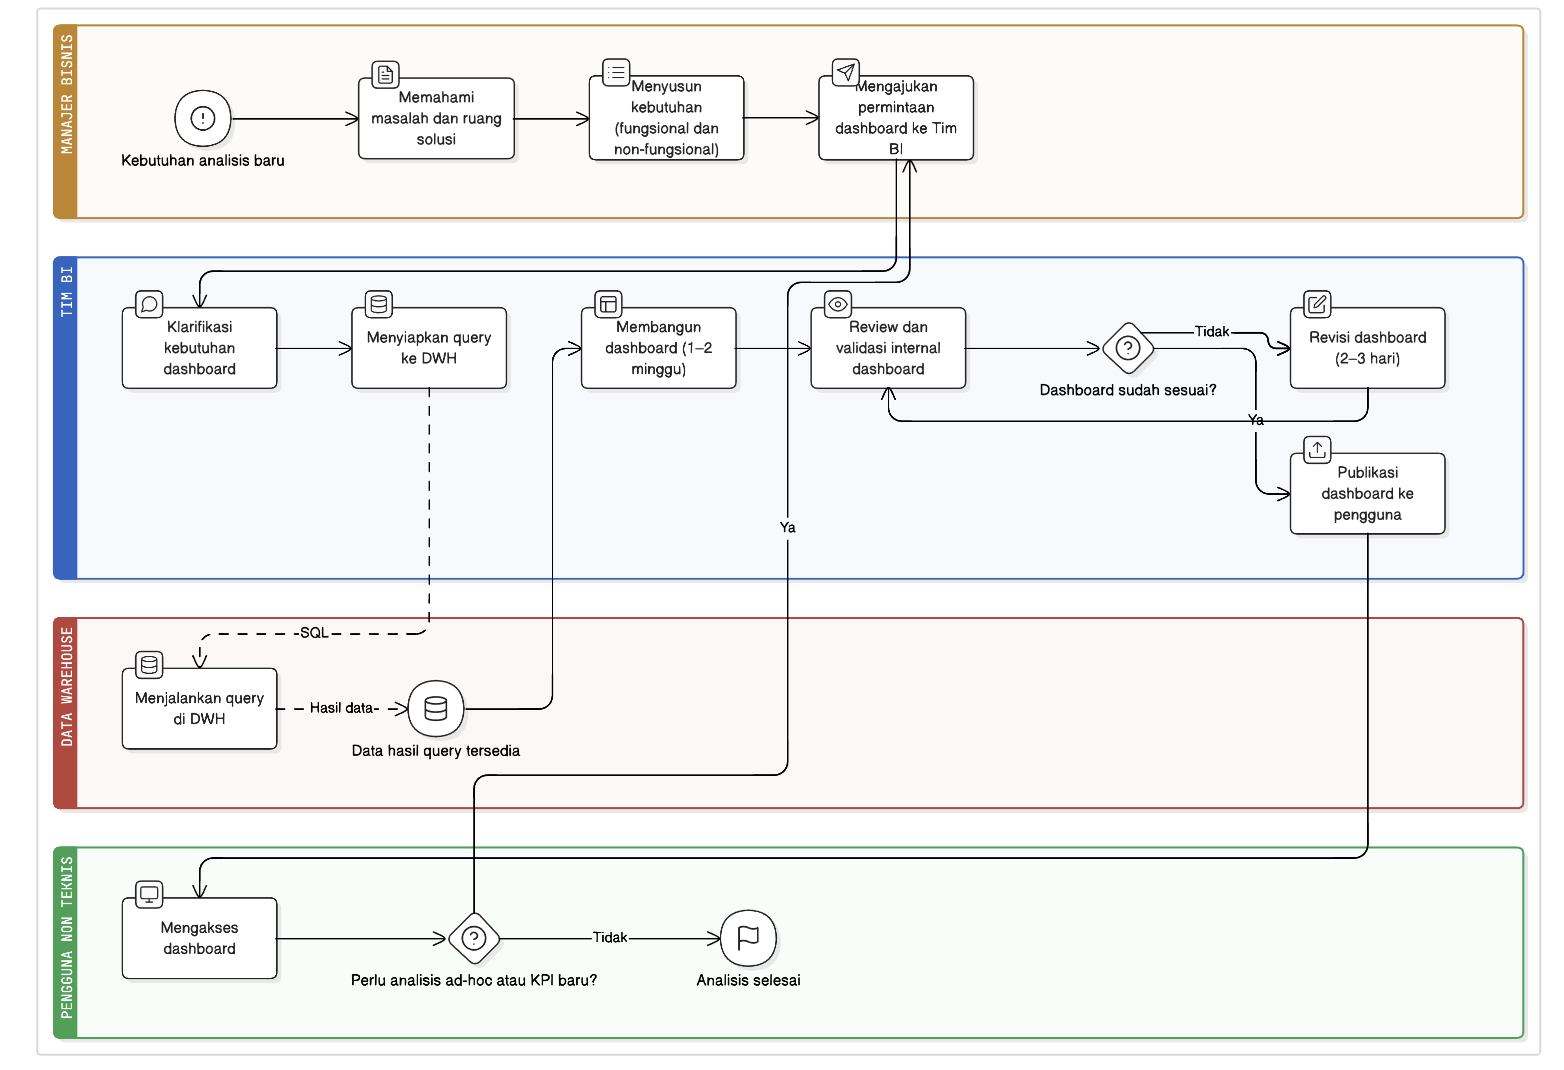
\includegraphics[width=1\textwidth,
                   height=1\textheight,
                   keepaspectratio]{images/bpmnasis}
  \caption{BPMN Sistem \textit{As-Is}}
  \label{fig:bpmnasis}
\end{figure}

Visualisasi proses \textit{as-is} menunjukkan kompleksitas dan iterasi yang terlibat dalam setiap siklus permintaan analitik. Pengguna bisnis harus menunggu beberapa tahap pemrosesan, \textit{review}, dan validasi sebelum hasil analisis dapat diakses. Aliran data bersifat linear dengan berbagai \textit{handoff} antar departemen sehingga menciptakan \textit{bottleneck} dan jeda yang signifikan. Pengalaman pengguna berpusat pada antarmuka \textit{dashboard} statis, tanpa kemampuan untuk melakukan eksplorasi data secara interaktif maupun berinteraksi melalui dialog percakapan yang natural.

\section{Alur Proses Bisnis Sistem Analitik dengan Chatbot BI (\textit{To-Be})}
\label{sec:tobe}

Proses bisnis sistem analitik yang diusulkan (\textit{to-be}) merepresentasikan tingkat otomatisasi dan optimasi yang signifikan dibandingkan proses \textit{as-is}. Proses dimulai ketika pengguna mengajukan pertanyaan dalam bahasa alami kepada sistem \textit{chatbot}, yang kemudian dilanjutkan dengan proses \textit{login} ke sistem \textit{BI chatbot} untuk keperluan autentikasi dan otorisasi pengguna. Setelah autentikasi berhasil, sistem membangun halaman dialog \textit{chatbot} sebagai antarmuka utama interaksi antara pengguna dan sistem yang bersifat \textit{AI-powered}. Tahap pemrosesan dimulai dengan klasifikasi maksud berbasis pola untuk mengidentifikasi jenis pertanyaan yang diajukan, apakah bersifat deskriptif, diagnostik, atau prediktif. Berdasarkan jenis \textit{intent} tersebut, sistem melakukan perutean (\textit{routing}) ke modul yang sesuai, yaitu untuk analisis deskriptif dan diagnostik, sistem menggunakan \textit{rule-based query engine} untuk menghasilkan dan mengeksekusi kueri terstruktur terhadap \textit{data warehouse}; sedangkan untuk analisis prediktif, sistem mengakses model \textit{forecasting} yang telah dilatih untuk menghasilkan prediksi sesuai dengan rentang waktu (\textit{time horizon}) dan parameter yang relevan. Setelah hasil analisis diperoleh, sistem melakukan perhitungan KPI dan agregasi data, kemudian menerapkan \textit{natural language generation} berbasis templat (\textit{template-based NLG}) untuk mengonversi keluaran numerik menjadi narasi dalam bahasa alami yang koheren dan mudah dipahami. Respons yang telah diformat dalam Bahasa Indonesia kemudian ditampilkan kembali kepada pengguna melalui antarmuka \textit{chatbot}, dan pada tahap akhir pengguna dapat mengakses \textit{dashboard} untuk melakukan \textit{ad-hoc analysis} atau pelacakan KPI tambahan apabila diperlukan, atau proses diakhiri ketika analisis dinyatakan selesai.

Keunggulan proses \textit{to-be} dibandingkan proses \textit{as-is} terletak pada beberapa aspek utama: \textbf{kecepatan eksekusi} yang jauh lebih tinggi (hitungan menit dibandingkan hari) berkat eksekusi kueri \textit{real-time}, \textbf{aksesibilitas yang lebih luas} karena tidak lagi memerlukan keahlian teknis SQL untuk mengakses \textit{insight}, \textbf{otomatisasi proses} yang mengurangi beban kerja manual tim teknis melalui pemanfaatan \textit{rule-based query} dan penanganan \textit{intent} otomatis, \textbf{kemampuan analitik yang diperluas} melalui integrasi komponen prediktif berbasis \textit{machine learning}, serta \textbf{pengalaman pengguna} yang lebih baik melalui antarmuka percakapan yang natural dan responsif. Secara keseluruhan, rancangan \textit{to-be} ini memungkinkan siklus permintaan hingga penyajian hasil analitik standar diselesaikan dalam waktu kurang dari satu menit untuk mayoritas kasus sehingga lebih selaras dengan kebutuhan pengambilan keputusan yang cepat dan berbasis data. Diagram BPMN yang menggambarkan proses \textit{to-be} disajikan pada Gambar~\ref{fig:bpmntobe}.

\begin{figure}[htbp] 
  \centering
  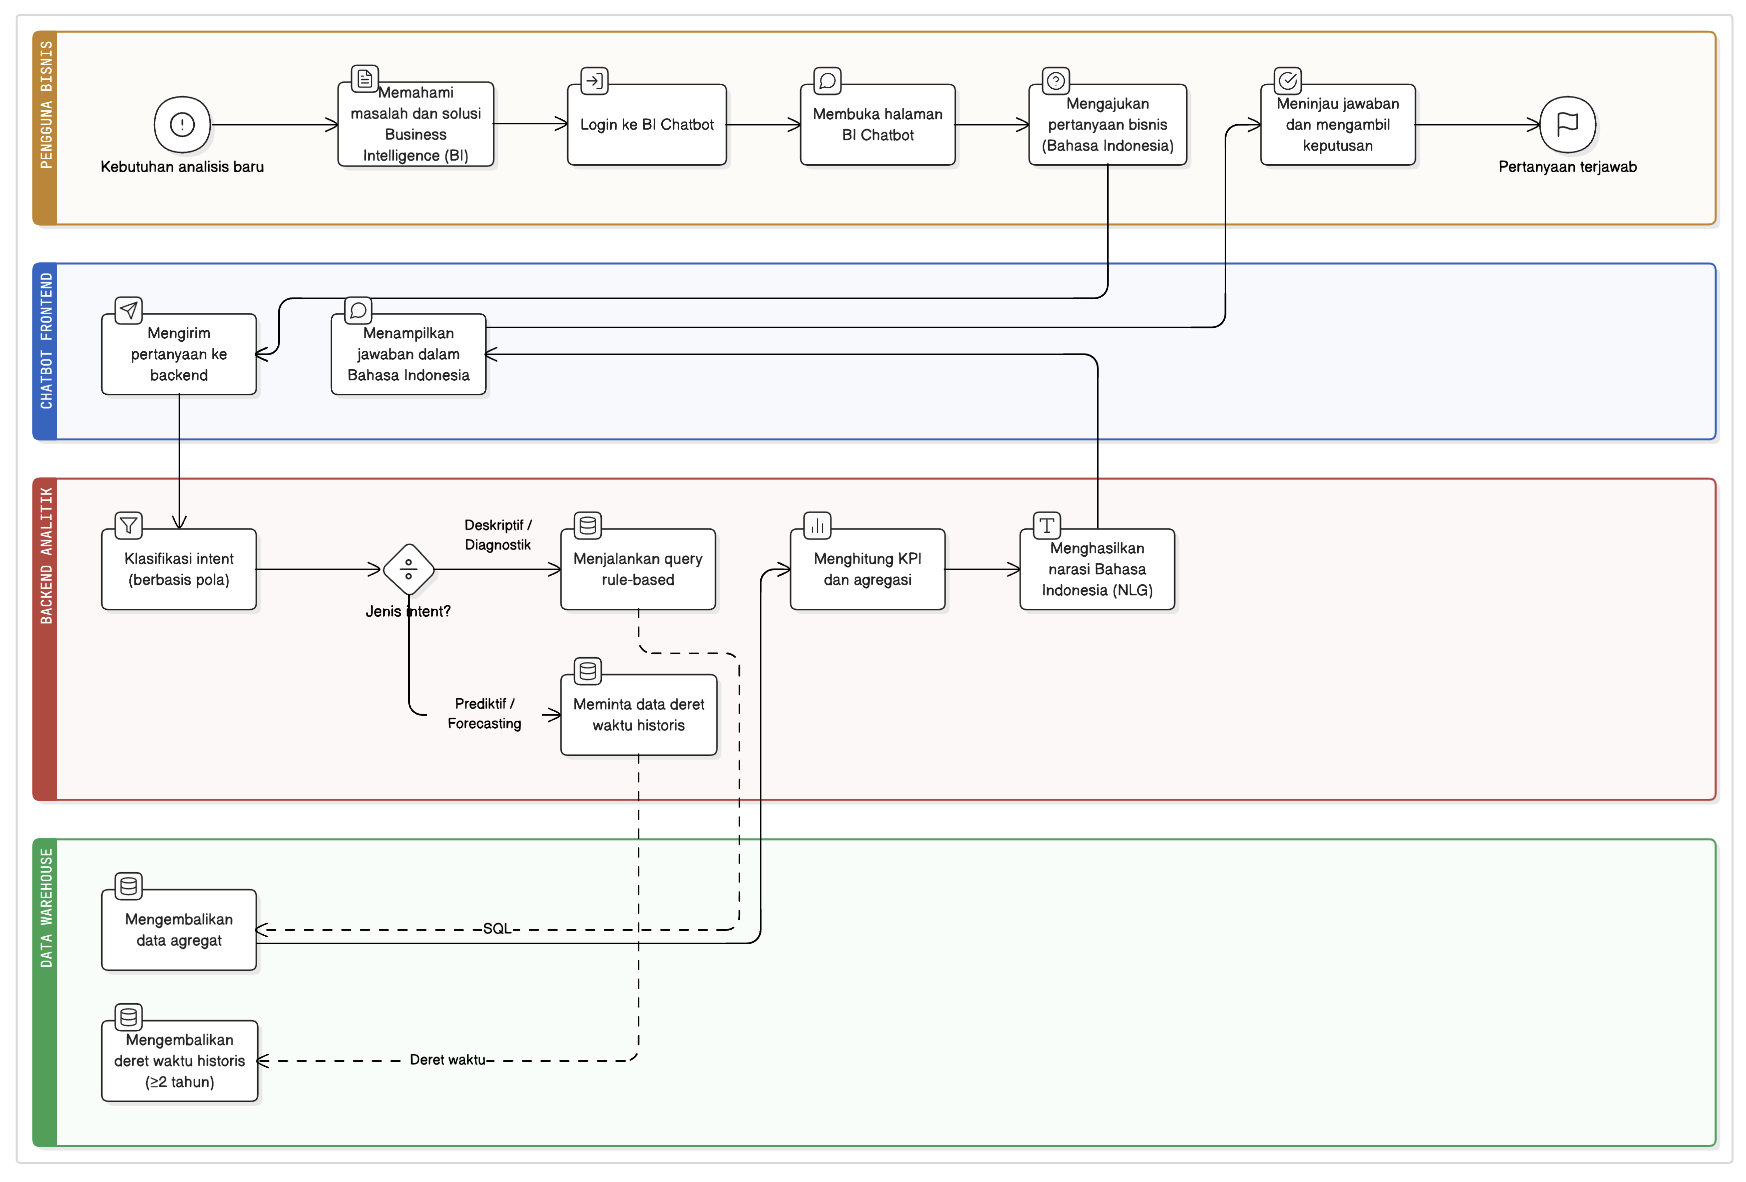
\includegraphics[width=1\textwidth,
                   height=1\textheight,
                   keepaspectratio]{images/bpmntobe}
  \caption{BPMN Sistem \textit{To-Be}}
  \label{fig:bpmntobe}
\end{figure}

Visualisasi proses \textit{to-be} menunjukkan peningkatan yang signifikan dalam efisiensi dan responsivitas sistem. Pengguna dapat secara langsung mengajukan pertanyaan melalui antarmuka \textit{chatbot} tanpa perlu menunggu atau melibatkan tim teknis. Aliran data bersifat paralel dengan otomatisasi penuh pada tahap pemrosesan sehingga memungkinkan hasil analisis diterima dalam waktu yang sangat singkat. Pengalaman pengguna berpusat pada dialog percakapan yang interaktif, dengan kemampuan untuk melakukan eksplorasi data secara \textit{real-time} serta mengajukan kueri lanjutan (\textit{follow-up queries}) secara mulus.

\section{Perbandingan Sistem Saat Ini (\textit{As-Is}) dan Sistem Baru (\textit{To-Be})}
\label{sec:perbandingan-asis-tobe}

Berdasarkan analisis proses bisnis yang telah diuraikan pada bagian sebelumnya, terdapat perbedaan fundamental antara sistem analitik saat ini (\textit{as-is}) dan sistem yang diusulkan (\textit{to-be}). Sistem \textit{as-is} mengandalkan pelaporan manual dengan keterlibatan tim teknis pada setiap tahap, sedangkan sistem \textit{to-be} mengotomatisasi sebagian besar proses melalui antarmuka percakapan berbasis \textit{chatbot}. Perbandingan kedua sistem berdasarkan aspek-aspek kritis disajikan pada Tabel~\ref{tab:perbandingan-asis-tobe}.

\begin{longtable}{|p{2.5cm}|p{5.5cm}|p{5.5cm}|}
\caption{Perbandingan Sistem \textit{As-Is} dan \textit{To-Be}} \label{tab:perbandingan-asis-tobe} \\
\hline
\textbf{Aspek} & \textbf{Sistem \textit{As-Is}} & \textbf{Sistem \textit{To-Be}} \\
\hline
\endfirsthead
\multicolumn{3}{c}{\tablename\ \thetable\ -- \textit{Lanjutan dari halaman sebelumnya}} \\
\hline
\textbf{Aspek} & \textbf{Sistem \textit{As-Is}} & \textbf{Sistem \textit{To-Be}} \\
\hline
\endhead
\hline \multicolumn{3}{r}{\textit{Bersambung ke halaman berikutnya}} \\
\endfoot
\hline
\endlastfoot

Waktu Respons & 2--5 hari untuk kueri kompleks & $<$2 menit untuk 95\% kueri \\
\hline

Antarmuka Pengguna & \textit{Dashboard} statis, laporan manual & Antarmuka percakapan (\textit{chatbot}) dalam Bahasa Indonesia \\
\hline

Ketergantungan Teknis & Memerlukan tim TI/analis data untuk setiap permintaan & Pengguna nonteknis dapat mengakses \textit{insight} secara mandiri \\
\hline

Aksesibilitas & Terbatas pada pengguna dengan keahlian SQL & Seluruh pengguna internal dapat mengakses melalui bahasa alami \\
\hline

Kemampuan Analitik & Deskriptif dan diagnostik (historis) & Deskriptif, diagnostik, dan prediktif (\textit{forecasting}) \\
\hline

Proses Pengambilan Data & Ekstraksi manual dari berbagai sistem, transformasi via \textit{spreadsheet} & Otomatis melalui \textit{rule-based query engine} \\
\hline

Kemampuan Prediktif & Tidak tersedia atau dilakukan manual secara periodik & Terintegrasi dengan model \textit{time series forecasting} (LSTM/GRU/Prophet/ARIMA) \\
\hline

Format Respons & Tabel, grafik, laporan tertulis & Narasi bahasa alami (\textit{template-based NLG}) dengan visualisasi pendukung \\
\hline

Siklus \textit{Feedback} & Iteratif dan panjang dengan banyak \textit{handoff} & \textit{Real-time} dengan kemampuan kueri lanjutan \\
\hline

Skalabilitas & Terbatas oleh kapasitas tim teknis & Skala horizontal melalui arsitektur layanan mikro \\
\hline

Ketersediaan & Jam kerja (bergantung pada tim teknis) & Diakses setiap saat (\textit{self-service}) \\
\hline

\end{longtable}


\section{Rancangan Solusi Keseluruhan}
\label{sec:rancangan-solusi}

Rancangan solusi keseluruhan mengintegrasikan lima lapisan (\textit{layer}) arsitektur yang saling terhubung, yakni lapisan presentasi (\textit{presentation layer}), lapisan aplikasi (\textit{application layer}), lapisan logika bisnis (\textit{business logic layer}), lapisan data (\textit{data layer}), dan lapisan infrastruktur (\textit{infrastructure layer}). Integrasi kelima lapisan tersebut memastikan bahwa sistem memiliki tingkat fleksibilitas, skalabilitas, dan kemudahan pemeliharaan (\textit{maintainability}) yang tinggi untuk mendukung pertumbuhan bisnis serta evolusi kebutuhan analitik di masa depan.

\subsection{Komponen-Komponen Utama Arsitektur}
\label{subsec:komponen-arsitektur}

Lapisan presentasi mencakup antarmuka pengguna yang dibangun dengan teknologi \textit{web} modern, dengan fokus pada antarmuka \textit{chatbot} berbasis \textit{web} yang mendukung interaksi waktu nyata (\textit{real-time}) dengan \textit{backend} sistem. Antarmuka ini diimplementasikan menggunakan kerangka kerja \textit{frontend} modern dengan pemanfaatan komunikasi asinkronus yang memungkinkan percakapan dua arah tanpa penundaan yang signifikan. Lapisan ini juga mencakup komponen untuk menampilkan visualisasi data, metrik interaktif, dan laporan yang terintegrasi dengan hasil analisis yang dihasilkan oleh \textit{backend}.

Lapisan aplikasi mengenkapsulasi logika inti sistem yang terdiri atas beberapa modul utama. Modul \textit{Natural Language Understanding} (NLU) bertanggung jawab untuk melakukan penguraian (\textit{parsing}) dan pemahaman terhadap masukan pengguna dalam bahasa alami. Modul manajemen dialog mengelola status percakapan dan menjaga koherensi dalam dialog multigiliran (\textit{multi-turn}). Modul pembangkitan respons menghasilkan tanggapan yang sesuai berdasarkan hasil analisis yang diterima dari lapisan logika bisnis. Di sisi lain, lapisan logika bisnis mencakup implementasi aturan bisnis yang telah didefinisikan, mesin klasifikasi maksud, mesin kueri berbasis aturan, model \textit{machine learning} untuk peramalan, serta repositori templat untuk NLG. Lapisan ini merupakan jantung sistem yang mengonversi maksud pengguna menjadi aksi teknis yang konkret dan menghasilkan wawasan berbasis data.

Lapisan data mencakup koneksi dan interaksi dengan \textit{Enterprise Data Warehouse} yang menyimpan data transaksional dan data utama, serta lapisan singgahan (\textit{cache}) untuk menyimpan hasil kueri yang sering diakses guna meningkatkan performa. Lapisan ini juga mencakup repositori untuk menyimpan model \textit{machine learning} yang telah dilatih, metadata mengenai sumber data, dan log audit untuk melacak seluruh interaksi pengguna dengan sistem. Lapisan infrastruktur mencakup komponen teknis yang mendukung operasional sistem secara keseluruhan, antara lain \textit{web server} untuk aplikasi \textit{chatbot}, infrastruktur API untuk penanganan permintaan, layanan pemantauan (\textit{monitoring}) dan pencatatan (\textit{logging}), serta komponen keamanan untuk autentikasi dan otorisasi pengguna.

\subsection{Arsitektur Sistem dan Aliran Data}
\label{subsec:arsitektur-aliran-data}

Arsitektur sistem secara keseluruhan dirancang dengan pendekatan modular berbasis layanan, dengan setiap komponen fungsional (seperti layanan \textit{chatbot}, layanan kueri, layanan peramalan, dan layanan NLG) diimplementasikan secara terpisah. Komunikasi antarkomponen dilakukan melalui API REST untuk memastikan keterikatan yang longgar (\textit{loose coupling}) dan tingkat ketahanan (\textit{resilience}) yang memadai terhadap gangguan.

Diagram arsitektur sistem yang lebih rinci disajikan pada Gambar~\ref{fig:arsitektur}, yang memperlihatkan integrasi kelima lapisan dan aliran data antarkomponen di dalam sistem. Arsitektur ini dirancang untuk mendukung:

\begin{enumerate}
    \item \textbf{Skalabilitas horizontal}, dengan setiap layanan dapat diduplikasi sesuai dengan kebutuhan kapasitas.
    \item \textbf{Ketahanan (\textit{Resilience})} sehingga kegagalan pada satu layanan tidak secara langsung menyebabkan kegagalan sistem secara keseluruhan.
    \item \textbf{Kemudahan Pemeliharaan} karena setiap modul dapat dikembangkan, diuji, dan di-\textit{deploy} secara independen.
    \item \textbf{Interoperabilitas}, melalui kemampuan setiap layanan untuk berinteraksi menggunakan standar API.
    \item \textbf{Keamanan}, dengan penerapan autentikasi berlapis dan enkripsi data.
\end{enumerate}

\begin{figure}[htbp] 
  \centering
  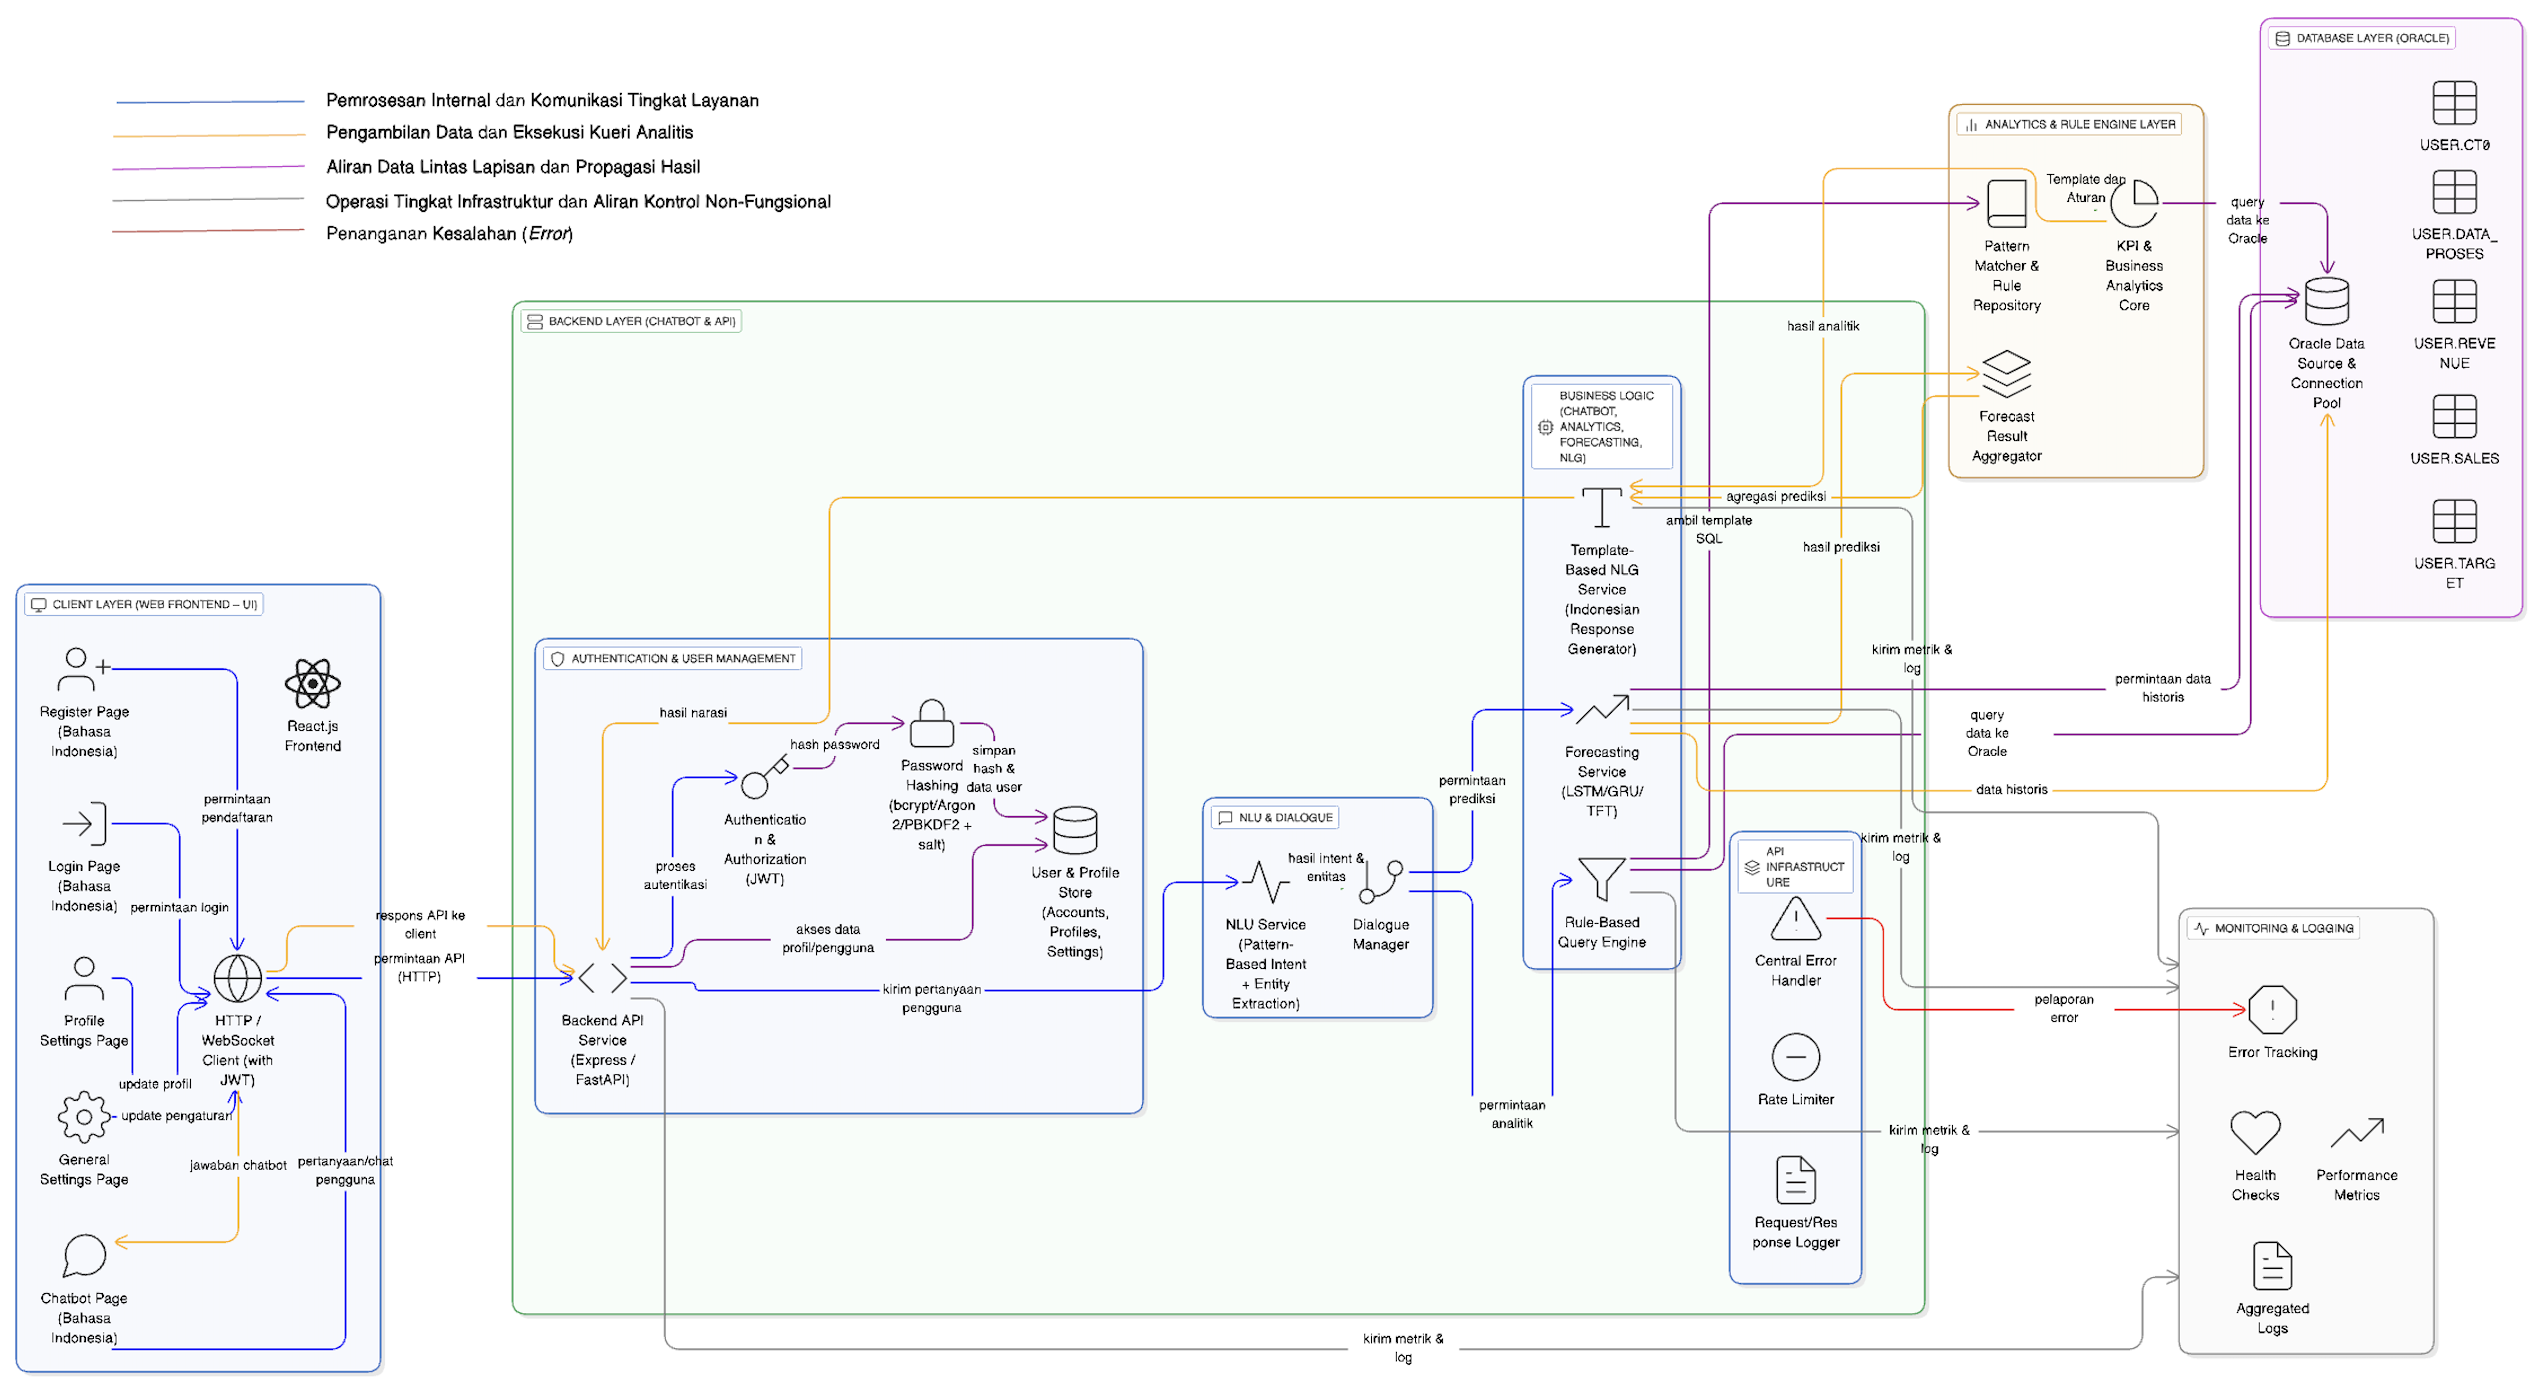
\includegraphics[width=1\textwidth,
                   height=1\textheight,
                   keepaspectratio]{images/arsitektur}
  \caption{Diagram Arsitektur Sistem Baru Secara Keseluruhan}
  \label{fig:arsitektur}
\end{figure}

Diagram arsitektur ini menggunakan sistem pewarnaan aliran untuk membedakan jenis interaksi yang terjadi antar komponen sehingga pembacaan terhadap alur kerja sistem menjadi lebih jelas. Aliran berwarna biru menggambarkan proses internal dan komunikasi tingkat layanan, yaitu interaksi antarmodul di dalam \textit{backend} seperti layanan autentikasi, modul klasifikasi maksud, manajemen dialog, mesin kueri berbasis aturan, serta layanan peramalan. Aliran berwarna oranye merepresentasikan proses pengambilan data dan eksekusi kueri analitik, khususnya komunikasi antara \textit{backend} dan \textit{Enterprise Data Warehouse} melalui sistem koneksi \textit{Oracle} untuk memperoleh data historis maupun metrik operasional yang relevan. Sementara itu, aliran berwarna ungu menunjukkan aliran data lintas lapisan dan propagasi hasil, yaitu bagaimana keluaran analitik dikembalikan ke lapisan logika bisnis untuk diproses lebih lanjut melalui mekanisme templating NLG. Aliran berwarna abu-abu menggambarkan operasi infrastruktur (seperti \textit{logging}, \textit{rate limiting}, pemantauan) yang dikelola oleh unit infrastruktur API guna menjaga keandalan sistem secara menyeluruh. Aliran berwarna merah digunakan untuk menandakan jalur penanganan kesalahan (\textit{error handling}). Melalui pemisahan aliran ini, diagram memberikan representasi yang lebih presisi mengenai bagaimana permintaan dari antarmuka diproses secara \textit{end-to-end}, mulai dari autentikasi, analisis \textit{intent}, eksekusi aturan, perhitungan prediktif, pengambilan data ke EDW, hingga penyusunan dan pengiriman kembali respons kepada pengguna.

Sebagai catatan komprehensif terhadap diagram arsitektur sistem di atas, komponen \textit{Temporal Fusion Transformer} (TFT) dicantumkan pada desain layanan peramalan sebagai bentuk rancangan sistem prediktif yang holistik. Akan tetapi, implementasi secara teknis pada penelitian ini difokuskan secara eksklusif pada pemodelan LSTM dan GRU. Model TFT diposisikan sebagai landasan teoretis untuk pengembangan iterasi sistem di masa mendatang mengingat tingginya kompleksitas komputasi serta besarnya kebutuhan volume data latih yang dipersyaratkan oleh arsitektur tersebut.

Dalam mencegah terjadinya latensi yang tinggi, aspek waktu respons ditetapkan sebagai salah satu metrik krusial dalam perancangan ini mengingat produk yang dikembangkan beroperasi pada level operasional dan harus mampu memberikan jawaban secara cepat terhadap permintaan analitik harian. Tantangan utama muncul dari karakteristik \textit{Enterprise Data Warehouse} yang menyimpan data dalam volume besar sehingga eksekusi kueri kompleks berpotensi menimbulkan penundaan. Dalam mengatasi hal tersebut, sistem menerapkan mekanisme optimasi, termasuk tembolok tingkat aturan (\textit{rule-level caching}) dengan pendekatan \textit{Time To Live} (TTL) yang memastikan hasil kueri disimpan sementara dan digunakan kembali tanpa perlu mengakses EDW setiap kali pengguna mengajukan permintaan yang sama. Kombinasi dari strategi ini memungkinkan penurunan latensi secara konsisten dan memastikan bahwa sistem tetap responsif dalam konteks penggunaan operasional.

\section{Kebutuhan Perangkat dan Lingkungan Sistem}
\label{sec:perangkat}

Dalam memastikan bahwa arsitektur yang dirancang dapat diimplementasikan dan direproduksi, sistem memerlukan spesifikasi perangkat lunak dan perangkat keras tertentu yang berfungsi sebagai fondasi dari pengembangan sistem (\textit{environment setup}).

\subsection{Perangkat Lunak dan Teknologi}
\label{subsec:tools}

Dalam melakukan implementasi dan pembangunan sistem yang nyata (tidak hanya sekadar rancangan), dibutuhkan beberapa perangkat lunak, pustaka pemrograman (\textit{libraries}), dan teknologi pendukung. Daftar teknologi pada Tabel~\ref{tab:tools} merincikan versi dan fungsi spesifik setiap perangkat dalam sistem \textit{Business Intelligence Chatbot}. Penjabaran ini memastikan bahwa seluruh proses, dari akuisisi data, pelatihan model, hingga rekayasa fitur, dapat ditelusuri dan direproduksi secara akurat.

\begin{longtable}{|c|p{2.5cm}|p{9cm}|}
\caption{Perangkat Lunak dan Teknologi Implementasi Sistem} \label{tab:tools} \\
\hline
\textbf{No} & \textbf{Perangkat} & \textbf{Deskripsi} \\
\hline
\endfirsthead
\multicolumn{3}{c}%
{\tablename\ \thetable\ -- \textit{Lanjutan dari halaman sebelumnya}} \\
\hline
\textbf{No} & \textbf{Perangkat} & \textbf{Deskripsi} \\
\hline
\endhead
\hline \multicolumn{3}{r}{\textit{Bersambung ke halaman berikutnya}} \\
\endfoot
\hline
\endlastfoot

1 & Node.js & \textit{Runtime} JavaScript sisi pelayan yang digunakan sebagai \textit{backend} utama sistem. Node.js menjalankan Express.js untuk menyediakan \textit{RESTful API}, mengelola autentikasi pengguna, mengeksekusi mesin aturan (\textit{rule engine}), serta menghasilkan respons naratif melalui modul NLG berbasis templat JavaScript. \\
\hline

2 & Python & Bahasa pemrograman yang digunakan khusus untuk layanan \textit{machine learning} (\textit{ML Service}). Python menangani pelatihan dan inferensi model peramalan deret waktu berbasis GRU dan LSTM melalui \textit{framework} FastAPI. \\
\hline

3 & FastAPI & \textit{Framework} Python untuk membangun \textit{RESTful API} dengan performa tinggi dan dokumentasi otomatis (Swagger/OpenAPI). FastAPI digunakan khusus untuk layanan \textit{machine learning} yang menangani permintaan pelatihan dan prediksi model peramalan deret waktu. \\
\hline

4 & React.js & Pustaka JavaScript untuk membangun antarmuka pengguna yang interaktif dan responsif. React.js digunakan untuk mengembangkan \textit{frontend chatbot} berbasis web dengan fitur percakapan, panel peramalan, dan alur terpandu (\textit{guided flow}). \\
\hline

5 & Oracle Database & \textit{Enterprise Data Warehouse} (DWH) yang menjadi sumber data utama sistem. Oracle Database digunakan untuk dua tujuan: (1) menyimpan data pengguna, riwayat percakapan, dan sesi melalui \textit{connection pooling} dengan pustaka \texttt{node-oracledb}; dan (2) menyediakan data analitik bisnis dari skema \texttt{DWH\_MOIS} yang mencakup lima domain data (penjualan, pendapatan, target, proses data pelanggan, dan \textit{churn}). \\
\hline

6 & PyTorch & \textit{Framework deep learning} utama yang digunakan untuk membangun dan melatih model peramalan deret waktu berbasis GRU dan LSTM. PyTorch dipilih karena fleksibilitas dalam pendefinisian arsitektur model kustom dan kemudahan \textit{debugging}. \\
\hline

7 & Express.js & \textit{Framework} web minimalis untuk Node.js yang digunakan sebagai fondasi \textit{backend} utama. Express.js menangani \textit{routing}, \textit{middleware} keamanan (Helmet, CORS, \textit{rate limiter}), serta integrasi dengan mesin aturan dan modul NLG. \\
\hline

8 & Pandas & Pustaka Python untuk manipulasi dan analisis data tabular. Pandas digunakan pada tahap \textit{data preparation}, transformasi fitur, dan agregasi data sebelum proses pelatihan model maupun eksekusi kueri. \\
\hline

9 & NumPy & Pustaka Python untuk komputasi numerik yang menjadi fondasi operasi matematika pada pemrosesan data dan perhitungan metrik evaluasi model. \\
\hline

10 & Scikit-learn & Pustaka \textit{machine learning} Python yang digunakan untuk praolah data, ekstraksi fitur, perhitungan metrik evaluasi, dan implementasi model \textit{baseline} untuk perbandingan performa. \\
\hline

11 & \texttt{node-oracledb} & Pustaka Node.js resmi dari Oracle untuk koneksi ke Oracle Database. Pustaka ini mengelola \textit{connection pooling}, eksekusi kueri SQL, dan penanganan tipe data khusus Oracle seperti CLOB. \\
\hline

12 & Regex (JavaScript) & Modul ekspresi reguler bawaan JavaScript yang digunakan untuk implementasi pencocokan pola (\textit{pattern matching}) dalam klasifikasi maksud berbasis aturan dan ekstraksi konteks geografis dari kueri pengguna. \\
\hline

13 & Pustaka Templat JavaScript & Modul templat kustom yang dibangun dalam JavaScript untuk implementasi \textit{template-based Natural Language Generation}. Modul ini mendukung lebih dari 30 subjek aturan dengan variasi templat per \textit{intent} yang diisi secara dinamis berdasarkan data hasil kueri Oracle. \\
\hline

14 & JWT / bcrypt & Pustaka keamanan yang digunakan untuk autentikasi berbasis \textit{JSON Web Token} (JWT) dan enkripsi kata sandi menggunakan algoritma \textit{bcrypt} dengan \textit{salt rounds}. \\
\hline

15 & Git / GitHub & Sistem kontrol versi dan platform kolaborasi yang digunakan untuk manajemen kode sumber, pelacakan perubahan, dan dokumentasi proyek tugas akhir. \\
\hline

16 & Jupyter Notebook & Aplikasi \textit{open-source} yang digunakan untuk eksplorasi data, eksperimen model, dan dokumentasi proses analisis dalam format dokumen interaktif yang menggabungkan kode, visualisasi, dan narasi. \\
\hline

17 & Google Colaboratory & Platform \textit{cloud} dari Google yang menyediakan akses gratis ke GPU untuk pelatihan model \textit{deep learning}. Google Colab digunakan untuk melatih model peramalan deret waktu yang memerlukan komputasi intensif. \\
\hline

18 & Postman & Aplikasi untuk pengujian dan dokumentasi API. Postman digunakan untuk menguji \textit{endpoint} API \textit{backend} sistem dan memvalidasi respons sebelum integrasi dengan \textit{frontend}. \\
\hline

19 & Visual Studio Code & \textit{Integrated Development Environment} (IDE) yang digunakan untuk penulisan kode, \textit{debugging}, dan manajemen proyek pengembangan sistem. \\
\hline

\end{longtable}


\subsection{Kebutuhan Sumber Daya Komputasi}
\label{subsec:resources}

Dalam mendukung proses pelatihan model \textit{deep learning} dan pengujian arsitektur yang diusulkan, diperlukan sumber daya komputasi yang memadai. Pelatihan model peramalan deret waktu berbasis LSTM dan GRU memerlukan akselerasi GPU untuk mempercepat proses komputasi yang kompleks. Pengembangan sistem ini memanfaatkan Google Colaboratory yang menyediakan akses ke GPU NVIDIA T4 dengan kapasitas 15GB memori GPU. 

Dalam tahap implementasi dan peluncuran produk secara langsung (\textit{deployment}), infrastruktur peladen (\textit{server}) dirancang untuk memiliki spesifikasi minimal 4 inti prosesor (\textit{cores}), memori RAM sebesar 16GB, dan penyimpanan berbasis SSD minimal 100GB guna memastikan aliran data yang cepat tanpa \textit{bottleneck} pada sistem berkas. 

\section{Desain Pengujian dan Evaluasi}
\label{sec:evaluasi}

Dalam memastikan bahwa sistem yang dikembangkan memenuhi spesifikasi dari desain arsitektur yang diajukan dan menguji keberhasilan implementasi, dirancang strategi pengujian dan evaluasi. Evaluasi ini mencakup penyelesaian bagian-bagian inti yang paling menantang dari sistem: modul klasifikasi maksud berbasis pola, pembangkitan bahasa alami (NLG), dan performa prediksi deret waktu.

\subsection{Evaluasi Klasifikasi Maksud Berbasis Pola}
\label{subsec:eval-intent}

Modul pencocokan kueri ke aturan bisnis dievaluasi menggunakan metrik standar klasifikasi multi-kelas. Sistem mengimplementasikan tujuh kategori \textit{intent} yang dipetakan ke 38 aturan bisnis; evaluasi dilakukan pada level pencocokan aturan (38 kelas) dengan pendekatan \textit{one-vs-all} dan agregasi metrik menggunakan strategi \textit{macro-averaging}, \textit{micro-averaging}, dan \textit{weighted-averaging}.

\subsubsection{Metrik Evaluasi Klasifikasi \textit{Intent}}

Metrik evaluasi yang digunakan untuk mengukur performa klasifikasi maksud mencakup:

\begin{enumerate}
    \item \textbf{Akurasi (\textit{Accuracy})}: Proporsi prediksi yang benar dari keseluruhan prediksi. Target minimal adalah 85\%.
    \item \textbf{Presisi (\textit{Precision})}: Proporsi prediksi positif yang benar dari seluruh prediksi positif. Dihitung per kelas kemudian diagregasi.
    \item \textbf{Daya Ingat (\textit{Recall})}: Proporsi sampel positif yang berhasil diprediksi benar dari seluruh sampel positif aktual.
    \item \textbf{Skor-F1 (\textit{F1-Score})}: Rata-rata harmonik dari presisi dan daya ingat, memberikan keseimbangan antara kedua metrik.
\end{enumerate}

Formula perhitungan metrik agregasi adalah sebagai berikut.

\begin{equation}
\label{sym:K}
\text{Presisi}_{\text{makro}} = \frac{1}{K} \sum_{i=1}^{K} \text{Presisi}_i
\end{equation}
\eqcaption{Presisi Makro}

\begin{equation}
\text{Daya Ingat}_{\text{makro}} = \frac{1}{K} \sum_{i=1}^{K} \text{Daya Ingat}_i
\end{equation}
\eqcaption{Daya Ingat Makro}

\begin{equation}
\text{Skor-F1}_{\text{makro}} = \frac{1}{K} \sum_{i=1}^{K} \text{Skor-F1}_i
\end{equation}
\eqcaption{Skor-F1 Makro}

dengan $K$ adalah jumlah kelas \textit{intent} dalam sistem.

\subsubsection{Analisis Nilai Keyakinan (\textit{Confidence Score})}

Sistem menggunakan mekanisme pemberian nilai keyakinan dalam rentang 0 hingga 100 untuk setiap prediksi klasifikasi maksud. Nilai dihitung melalui fungsi penjumlah bobot kata kunci primer dan pendukung yang cocok ($c = \min(100,\;\text{skor} \times 10)$). Ambang batas (\textit{threshold}) ditetapkan pada nilai 40 dengan ketentuan:
\begin{enumerate}
    \item Jika nilai keyakinan $\geq$ 40: Prediksi dianggap valid.
    \item Jika nilai keyakinan $<$ 40: Sistem meminta klarifikasi (\textit{fallback mechanism}).
\end{enumerate}

\subsection{Evaluasi Pembangkitan Bahasa Alami Berbasis Templat}
\label{subsec:eval-nlg}

Modul \textit{Natural Language Generation} (NLG) dievaluasi dari dua aspek: akurasi faktual dan evaluasi subjektif oleh pengguna internal.

\subsubsection{Akurasi Faktual}

Akurasi faktual dievaluasi dengan memverifikasi apakah seluruh nilai numerik dan informasi bisnis dalam respons NLG sesuai dengan hasil kueri dari basis data. Karena pendekatan NLG berbasis templat bersifat deterministik dan menyisipkan data langsung dari hasil kueri tanpa proses generatif, akurasi faktual dijamin secara arsitektural (Target: 100\%).

\subsubsection{Evaluasi Subjektif Berbasis Pengguna}

Kualitas keluaran NLG dinilai secara subjektif oleh pengguna internal perusahaan menggunakan kuesioner berskala Likert 1--5 pada empat dimensi utama:
\begin{enumerate}
    \item \textbf{Ketepatan Respons}: Menilai apakah jawaban yang diberikan sistem sesuai dengan data aktual.
    \item \textbf{Kejelasan Narasi}: Menilai apakah narasi, tabel, dan penjelasan yang dihasilkan sistem mudah dipahami.
    \item \textbf{Relevansi Analisis}: Menilai apakah \textit{insight} atau analisis yang diberikan sistem relevan dengan konteks pertanyaan pengguna.
    \item \textbf{Kemudahan Penggunaan}: Menilai apakah antarmuka dan alur interaksi sistem bersifat intuitif.
\end{enumerate}

\subsection{Evaluasi Peramalan Deret Waktu}
\label{subsec:eval-forecasting}

Model dievaluasi menggunakan protokol \textit{rolling-origin backtesting} untuk mencegah \textit{data leakage}. Evaluasi mencakup \textit{baseline} (ARIMA, Prophet) dan model utama (LSTM, GRU).

\begin{enumerate}
    \item \textbf{MAE (\textit{Mean Absolute Error})}: Rata-rata nilai absolut selisih prediksi dan aktual.
    \item \textbf{RMSE (\textit{Root Mean Squared Error})}: Akar kuadrat rata-rata kuadrat selisih.
    \item \textbf{sMAPE (\textit{Symmetric Mean Absolute Percentage Error})}:
    \begin{equation}
    \text{sMAPE} = \frac{100\%}{n} \sum_{i=1}^{n} \frac{|y_i - \hat{y}_i|}{(|y_i| + |\hat{y}_i|)/2}
    \end{equation}
    \eqcaption{sMAPE}

    \item \textbf{MASE (\textit{Mean Absolute Scaled Error})}:
    \begin{equation}
    \text{MASE} = \frac{\text{MAE}}{\frac{1}{n-1} \sum_{i=2}^{n} |y_i - y_{i-1}|}
    \end{equation}
    \eqcaption{MASE}
\end{enumerate}

Dalam mengukur peningkatan performa model terhadap garis dasar (\textit{seasonal naive}), dihitung \textit{skill score}:
\begin{equation}
\text{\textit{Skill Score}} = 1 - \frac{\text{MAE}_{\text{model}}}{\text{MAE}_{\text{baseline}}}
\end{equation}
\eqcaption{\textit{Skill Score}}


% ==========================================
% BAB V IMPLEMENTASI
% ==========================================
\cleardoublepage
\chapter{IMPLEMENTASI SISTEM \textit{BUSINESS INTELLIGENCE CHATBOT}}
\label{chap:implementasi}

Bab ini menyajikan implementasi sistem \textit{Business Intelligence} berbasis \textit{rule-based chatbot} yang telah dirancang pada bab sebelumnya. Pembahasan mencakup arsitektur sistem yang diimplementasikan, implementasi setiap komponen utama, serta integrasi antar-komponen menjadi satu kesatuan sistem yang fungsional.

\section{Arsitektur Sistem Terimplementasi}
\label{sec:arsitektur-terimplementasi}

Sistem BrightAI diimplementasikan dengan arsitektur tiga lapis (\textit{three-tier architecture}) yang memisahkan tanggung jawab setiap komponen secara jelas. Ketiga lapis tersebut adalah sebagai berikut.

\begin{enumerate}
    \item \textbf{\textit{Frontend} (React.js)}: Antarmuka pengguna berbasis web yang menyediakan fitur percakapan \textit{chatbot}, panel peramalan, dan manajemen profil pengguna. \textit{Frontend} berjalan pada porta 3000 dan berkomunikasi dengan \textit{backend} melalui \textit{RESTful API}.
    \item \textbf{\textit{Backend} (Node.js/Express)}: Peladen utama yang menangani autentikasi, manajemen sesi, eksekusi mesin aturan (\textit{rule engine}), klasifikasi maksud (\textit{intent classification}), pembangkitan bahasa alami (NLG), serta komunikasi dengan basis data Oracle. \textit{Backend} berjalan pada porta 3001.
    \item \textbf{Layanan \textit{Machine Learning} (FastAPI/PyTorch)}: Layanan terpisah yang menangani pelatihan dan inferensi model peramalan deret waktu berbasis GRU dan LSTM. Layanan ini berjalan pada porta 8000 dan diakses oleh \textit{backend} melalui permintaan HTTP internal.
\end{enumerate}

Ketiga lapis terhubung ke Oracle Database yang berfungsi ganda melalui dua skema terpisah: (1) skema \texttt{DWH\_MOIS} sebagai \textit{Enterprise Data Warehouse} (DWH)\label{abbr:DWH} yang menyimpan lima tabel domain analitik dengan prefiks \texttt{BRIGHTAI\_} (\texttt{BRIGHTAI\_SALES}, \texttt{BRIGHTAI\_REVENUE}, \texttt{BRIGHTAI\_TARGET}, \texttt{BRIGHTAI\_DAPROS}, \texttt{BRIGHTAI\_CT0\_NAL}); dan (2) skema \texttt{USR\_RPT} yang menyimpan data operasional sistem, meliputi tabel pengguna (\texttt{BRIGHTAI\_USER}), riwayat percakapan (\texttt{BRIGHTAI\_CHAT}), dan sesi (\texttt{BRIGHTAI\_SESSION}).

\section{Implementasi \textit{Backend} (Node.js/Express)}
\label{sec:impl-backend}

\textit{Backend} sistem diimplementasikan menggunakan Node.js dengan \textit{framework} Express.js sebagai fondasi \textit{RESTful API}. Berkas utama \texttt{server.js} menginisialisasi aplikasi Express, mengonfigurasi \textit{middleware}, mendaftarkan rute API, serta mengelola siklus hidup koneksi basis data.

\subsection{Struktur Proyek \textit{Backend}}

Proyek \textit{backend} diorganisasi menggunakan pola arsitektur MVC (\textit{Model-View-Controller}) yang dimodifikasi menjadi struktur berlapis. Tabel~\ref{tab:struktur-backend} menyajikan struktur direktori utama.

\begin{longtable}{|p{4.5cm}|p{8.5cm}|}
\caption{Struktur Direktori Proyek \textit{Backend}} \label{tab:struktur-backend} \\
\hline
\textbf{Direktori/Berkas} & \textbf{Fungsi} \\
\hline
\endfirsthead
\hline
\textbf{Direktori/Berkas} & \textbf{Fungsi} \\
\hline
\endhead
\hline
\endfoot
\texttt{server.js} & Titik masuk utama aplikasi: inisialisasi Express, \textit{middleware}, rute, dan koneksi basis data \\
\hline
\texttt{config/database.js} & Konfigurasi koneksi Oracle Database, \textit{connection pooling}, dan eksekutor kueri \\
\hline
\texttt{src/controllers/} & Penangan permintaan (\textit{request handler}): \texttt{authController.js} dan \texttt{chatController.js} \\
\hline
\texttt{src/models/} & Model data untuk pengguna, riwayat percakapan, dan sesi \\
\hline
\texttt{src/routes/} & Definisi rute API: autentikasi, \textit{chat}, sesi, dan peramalan \\
\hline
\texttt{src/rules/engine/} & Mesin aturan, klasifikasi maksud, pemroses kueri, dan pembangkit bahasa alami \\
\hline
\texttt{src/rules/databases/} & Definisi aturan per domain basis data \\
\hline
\texttt{src/rules/config/} & Registri aturan dan konfigurasi pemetaan tabel \\
\hline
\texttt{src/middleware/} & \textit{Middleware} autentikasi JWT dan penanganan kesalahan \\
\hline
\texttt{src/utils/} & Utilitas: \textit{logger}, \textit{cache}, dan fungsi pembantu \\
\hline
\end{longtable}


\subsection{Konfigurasi \textit{Middleware} Keamanan}

Sistem mengimplementasikan beberapa lapisan \textit{middleware} keamanan pada Express.js untuk melindungi API dari ancaman umum. Konfigurasi \textit{middleware} yang diterapkan mencakup:

\begin{enumerate}
    \item \textbf{Helmet}: Mengatur tajuk HTTP keamanan (\textit{security headers}) untuk mencegah serangan seperti \textit{Cross-Site Scripting} (XSS) dan \textit{clickjacking}.
    \item \textbf{CORS\label{abbr:CORS} (\textit{Cross-Origin Resource Sharing})}: Mengizinkan permintaan lintas-asal dari \textit{frontend} yang berjalan pada domain berbeda.
    \item \textbf{\textit{Rate Limiter}}: Membatasi jumlah permintaan per alamat IP menjadi maksimal 100 permintaan per 15 menit untuk mencegah serangan \textit{brute force} dan \textit{Denial of Service} (DoS).
    \item \textbf{Pembatasan Ukuran \textit{Payload}}: Membatasi ukuran badan permintaan JSON menjadi maksimal 10 MB.
\end{enumerate}

\subsection{Koneksi Oracle Database}
\label{subsec:koneksi-oracle}

Koneksi ke Oracle Database dikelola melalui modul \texttt{config/database.js} menggunakan pustaka \texttt{node-oracledb}. Satu \textit{connection pool} melayani akses ke kedua skema: \texttt{DWH\_MOIS} untuk kueri analitik dan \texttt{USR\_RPT} untuk operasi autentikasi serta manajemen sesi. Konfigurasi \textit{pool} disajikan pada Tabel~\ref{tab:pool-config}.

\begin{table}[h]
\centering
\caption{Konfigurasi \textit{Connection Pool} Oracle Database}
\label{tab:pool-config}
\begin{tabular}{|p{4cm}|c|p{6cm}|}
\hline
\textbf{Parameter} & \textbf{Nilai} & \textbf{Keterangan} \\
\hline
\texttt{poolMin} & 2 & Jumlah koneksi minimum yang dipertahankan \\
\hline
\texttt{poolMax} & 10 & Jumlah koneksi maksimum yang diizinkan \\
\hline
\texttt{poolIncrement} & 1 & Penambahan koneksi per permintaan baru \\
\hline
\texttt{connectTimeout} & 10 detik & Batas waktu koneksi awal \\
\hline
\end{tabular}
\end{table}

Modul ini juga menyediakan fungsi \texttt{executeQuery} yang menangani eksekusi kueri SQL dengan format keluaran objek (\texttt{OUT\_FORMAT\_OBJECT}), penanganan tipe data CLOB secara otomatis, serta penutupan koneksi yang aman melalui blok \texttt{finally}. Setiap baris hasil kueri yang mengandung CLOB diproses secara asinkron menggunakan \textit{stream} untuk mencegah kebocoran memori.

\subsection{Rute API (\textit{API Routes})}

\textit{Backend} menyediakan empat kelompok rute API utama yang disajikan pada Tabel~\ref{tab:api-routes}.

\begin{longtable}{|p{1.5cm}|p{4cm}|p{7cm}|}
\caption{Rute API Sistem BrightAI} \label{tab:api-routes} \\
\hline
\textbf{Metode} & \textbf{\textit{Endpoint}} & \textbf{Fungsi} \\
\hline
\endfirsthead
\hline
\textbf{Metode} & \textbf{\textit{Endpoint}} & \textbf{Fungsi} \\
\hline
\endhead
\hline
\endfoot
POST & \texttt{/api/auth/register} & Registrasi pengguna baru \\
\hline
POST & \texttt{/api/auth/login} & Autentikasi dan penerbitan token JWT \\
\hline
GET & \texttt{/api/auth/profile} & Mengambil profil pengguna (memerlukan token) \\
\hline
PUT & \texttt{/api/auth/profile} & Memperbarui profil pengguna \\
\hline
PUT & \texttt{/api/auth/password} & Mengubah kata sandi \\
\hline
POST & \texttt{/api/chat/message} & Mengirim pesan ke \textit{chatbot} dan menerima respons \\
\hline
GET & \texttt{/api/chat/history} & Mengambil riwayat percakapan pengguna \\
\hline
GET & \texttt{/api/chat/session/:id} & Mengambil pesan dalam satu sesi percakapan \\
\hline
DELETE & \texttt{/api/chat/history} & Menghapus riwayat percakapan \\
\hline
GET & \texttt{/api/chat/capabilities} & Mengambil daftar kemampuan dan aturan yang tersedia \\
\hline
GET & \texttt{/api/sessions} & Mengambil daftar sesi percakapan \\
\hline
POST & \texttt{/api/forecast/*} & Meneruskan permintaan peramalan ke layanan ML \\
\hline
GET & \texttt{/api/telkom/health} & Pemeriksaan kesehatan (\textit{health check}) sistem \\
\hline
\end{longtable}


\section{Implementasi Mesin Aturan (\textit{Rule Engine})}
\label{sec:impl-rule-engine}

Mesin aturan merupakan komponen inti yang menghubungkan pertanyaan pengguna dengan kueri basis data dan respons naratif. Implementasi mesin aturan terdiri dari empat modul utama yang bekerja secara berurutan.

\subsection{Arsitektur Mesin Aturan}

Alur pemrosesan kueri dalam mesin aturan mengikuti tahapan sebagai berikut.

\begin{enumerate}
    \item \textbf{Penerimaan Kueri}: Modul \texttt{chatController.js} menerima pesan pengguna dan memeriksa apakah pesan tersebut merupakan sapaan, permintaan bantuan, atau kueri analitik.
    \item \textbf{Pencocokan Aturan}: Modul \texttt{queryProcessor.js} mencocokkan kueri pengguna dengan aturan yang tersedia menggunakan pencocokan pola kata kunci.
    \item \textbf{Eksekusi Aturan}: Modul \texttt{ruleEngine.js} mengeksekusi kueri SQL yang terkait dengan aturan yang cocok terhadap Oracle Database, dengan injeksi filter geografis secara dinamis.
    \item \textbf{Pembangunan Respons}: Modul \texttt{responseBuilder.js} dan \texttt{nlgGenerator.js} mengonversi hasil kueri menjadi narasi dalam bahasa Indonesia.
\end{enumerate}

\subsection{Struktur Definisi Aturan}

Setiap aturan didefinisikan sebagai objek JavaScript yang memiliki struktur terstandar. Komponen utama setiap aturan disajikan pada Tabel~\ref{tab:struktur-rule}.

\begin{table}[h]
\centering
\caption{Komponen Struktur Definisi Aturan}
\label{tab:struktur-rule}
\begin{tabular}{|p{3.5cm}|p{9cm}|}
\hline
\textbf{Komponen} & \textbf{Deskripsi} \\
\hline
\texttt{RULE\_META} & Metadata aturan: identifikasi (\texttt{RULE\_ID}), nama, deskripsi, domain basis data, kategori, dan prioritas eksekusi \\
\hline
\texttt{KEYWORDS} & Daftar kata kunci dan pola yang digunakan untuk mencocokkan kueri pengguna dengan aturan \\
\hline
\texttt{SQL\_QUERY} & Kueri SQL yang dieksekusi terhadap \textit{Enterprise Data Warehouse} Oracle (skema \texttt{DWH\_MOIS}) \\
\hline
\texttt{DATABASE\_CONFIG} & Konfigurasi tabel dan koneksi basis data yang digunakan oleh aturan \\
\hline
\texttt{BUSINESS\_LOGIC} & Fungsi pemrosesan logika bisnis, termasuk \texttt{formatIndonesianResponse} untuk mengubah data mentah menjadi struktur terformat \\
\hline
\texttt{CACHE\_DURATION} & Durasi penyimpanan hasil kueri dalam \textit{cache} (dalam detik) \\
\hline
\end{tabular}
\end{table}

Sistem mendukung 38 aturan analitik yang tersebar di lima tabel domain pada skema \texttt{DWH\_MOIS}, yaitu \texttt{BRIGHTAI\_SALES}, \texttt{BRIGHTAI\_REVENUE}, \texttt{BRIGHTAI\_TARGET}, \texttt{BRIGHTAI\_DAPROS}, dan \texttt{BRIGHTAI\_CT0\_NAL}. \textit{Listing}~\ref{lst:rule-definition} menyajikan contoh implementasi struktur definisi aturan secara lengkap.

\begin{lstlisting}[caption={Contoh Struktur Definisi Aturan Analitik}, label={lst:rule-definition}, style=jsstyle]
module.exports = {
  RULE_META: {
    RULE_ID: 'ps_001',
    RULE_NAME: 'total_order_hsi',
    DESCRIPTION: 'Analisis total order HSI bisnis dan basic',
    DATABASE: 'BRIGHTAI_SALES',
    CATEGORY: 'order_analysis',
    COMPLEXITY: 'MEDIUM',
    EXECUTION_PRIORITY: 'HIGH'
  },

  DATABASE_CONFIG: loadRuleDatabase("BRIGHTAI_SALES"),

  KEYWORD_PATTERNS: {
    primary: [
      'total order hsi', 'jumlah order', 'order hsi bisnis'
    ],
    supporting: [
      'order', 'hsi', 'bisnis', 'basic', 'bulanan'
    ],
    calculateConfidence: function(input) {
      const lowerInput = input.toLowerCase();
      const primaryMatches = this.primary.filter(
        kw => lowerInput.includes(kw)
      ).length;
      const supportingMatches = this.supporting.filter(
        kw => lowerInput.includes(kw)
      ).length;
      if (primaryMatches > 0)
        return Math.min(80 + primaryMatches*10
                        + supportingMatches*3, 100);
      if (supportingMatches >= 3)
        return 65 + supportingMatches * 4;
      return 0;
    }
  },

  SQL_QUERY: `SELECT ... FROM DWH_MOIS.BRIGHTAI_SALES
              WHERE GROUP4 = 'High Speed Internet' ...`,

  BUSINESS_LOGIC: {
    formatIndonesianResponse: function(data) {
      // Mengubah data mentah menjadi struktur terformat
      return { ringkasan: '...', metrik: {...} };
    }
  }
};
\end{lstlisting}


\subsection{Injeksi Filter Geografis}

Mesin aturan mengimplementasikan fitur injeksi filter geografis secara dinamis ke dalam kueri SQL pada saat eksekusi. Fitur ini memungkinkan pengguna menyaring data berdasarkan regional atau wilayah telekomunikasi (\textit{witel}) tanpa memerlukan aturan terpisah untuk setiap wilayah. Mekanisme injeksi mendukung dua mode:

\begin{enumerate}
    \item \textbf{Mode Penampung (\textit{placeholder})}: Jika kueri SQL mengandung penanda \texttt{/* :GEO\_FILTER: */}, penanda tersebut diganti dengan klausa filter yang sesuai.
    \item \textbf{Mode Injeksi Otomatis}: Jika tidak ada penanda, sistem melakukan pemindaian baris demi baris untuk menemukan blok \texttt{FROM DWH\_MOIS} dan menyisipkan klausa filter pada posisi yang tepat sebelum \texttt{GROUP BY} atau penutup subkueri.
\end{enumerate}

Algoritma~\ref{alg:geo-filter} mendeskripsikan prosedur lengkap deteksi cakupan geografis dan injeksi filter ke dalam kueri SQL.

\begin{algorithm}[H]
\caption{Injeksi Filter Geografis ke dalam Kueri SQL}
\label{alg:geo-filter}
\begin{algorithmic}[1]
\Require Masukan pengguna $q$, kueri SQL $S$, basis data $D$, pemetaan kolom $\mathcal{C}$
\Ensure Kueri SQL dengan filter geografis $S'$

\State $q_{\text{lower}} \gets \texttt{toLowerCase}(q)$

\State \textbf{// Tahap 1: Deteksi cakupan geografis}
\If{$q_{\text{lower}}$ mengandung kata kunci nasional}
    \State \Return $S$ \Comment{Tidak diperlukan filter — cakupan nasional}
\EndIf

\State $\textit{scope} \gets \texttt{null}$, $\textit{dbValue} \gets \texttt{null}$

\For{setiap pola $p$ dalam $\texttt{REGIONAL\_PATTERNS}$}
    \If{$q_{\text{lower}}$ mengandung $p.\textit{pattern}$}
        \State $\textit{scope} \gets \texttt{"regional"}$,\quad $\textit{dbValue} \gets p.\textit{dbValue}$
        \State \textbf{break}
    \EndIf
\EndFor

\If{$\textit{scope} = \texttt{null}$}
    \For{setiap pola $p$ dalam $\texttt{WITEL\_PATTERNS}$}
        \If{$q_{\text{lower}}$ mengandung $p.\textit{pattern}$}
            \State $\textit{scope} \gets \texttt{"witel"}$,\quad $\textit{dbValue} \gets p.\textit{dbValue}$
            \State \textbf{break}
        \EndIf
    \EndFor
\EndIf

\If{$\textit{scope} = \texttt{null}$ \textbf{atau} $\textit{dbValue} = \texttt{null}$}
    \State \Return $S$ \Comment{Tidak ada entitas geografis yang terdeteksi}
\EndIf

\State \textbf{// Tahap 2: Tentukan nama kolom sesuai basis data}
\State $\textit{cols} \gets \mathcal{C}[D]$ \Comment{Ambil pasangan \{regional, witel\} untuk $D$}
\State $\textit{colName} \gets \textit{cols}[\textit{scope}]$
\State $\textit{filterClause} \gets \texttt{"AND "} \| \textit{colName} \| \texttt{" = '"} \| \textit{dbValue} \| \texttt{"'"}$

\State \textbf{// Tahap 3: Injeksikan filter ke dalam SQL}
\If{$S$ mengandung \texttt{/* :GEO\_FILTER: */}}
    \State $S' \gets S.\texttt{replace}(\texttt{"/* :GEO\_FILTER: */"}, \textit{filterClause})$
    \State \Return $S'$
\EndIf

\State \textbf{// Tahap 3b: Injeksi otomatis jika tidak ada \textit{placeholder}}
\State Cari indeks baris \texttt{FROM DWH\_MOIS} pertama dalam $S$ $\to i_{\text{from}}$
\If{$i_{\text{from}} = -1$}
    \State \Return $S$
\EndIf
\State Cari indeks klausa \texttt{WHERE} setelah $i_{\text{from}}$ $\to i_{\text{where}}$
\If{$i_{\text{where}} = -1$}
    \State \Return $S$
\EndIf
\State Pindai baris dari $i_{\text{where}}$, lacak kedalaman tanda kurung $d \gets 0$
\For{setiap baris $\ell$ dari $i_{\text{where}}$ hingga akhir $S$}
    \State Perbarui $d$ berdasarkan karakter \texttt{(} dan \texttt{)} dalam $\ell$
    \If{$d < 0$ \textbf{atau} ($d = 0$ \textbf{dan} $\ell$ dimulai dengan \texttt{GROUP BY}/\texttt{ORDER BY}/\texttt{HAVING})}
        \State Sisipkan \textit{filterClause} sebelum baris $\ell$ dengan indentasi yang sama
        \State \Return $S'$
    \EndIf
\EndFor
\State \Return $S$

\end{algorithmic}
\end{algorithm}


\subsection{Mekanisme \textit{Caching}}

Hasil eksekusi aturan disimpan dalam \textit{cache} memori menggunakan kunci yang dihasilkan dari \textit{hash} MD5 kombinasi kueri pengguna dan konteks geografis. Setiap entri \textit{cache} memiliki durasi kedaluwarsa yang ditentukan oleh konfigurasi aturan (nilai bawaan: 1800 detik atau 30 menit). Mekanisme ini mengurangi beban kueri terhadap Oracle Database untuk pertanyaan yang sering diajukan.

\section{Implementasi Klasifikasi Maksud (\textit{Intent Classification})}
\label{sec:impl-intent}

Modul klasifikasi maksud diimplementasikan dalam berkas \texttt{intentClassifier.js} menggunakan pendekatan pencocokan pola kata kunci berbobot (\textit{weighted keyword matching}). Pendekatan ini dipilih karena memberikan latensi rendah (kurang dari 1 milidetik per kueri), interpretabilitas tinggi, dan kemampuan untuk bekerja dengan baik pada domain yang terbatas dan terdefinisi.

\subsection{Arsitektur Klasifikasi}

Sistem mengklasifikasikan setiap kueri pengguna ke dalam dua dimensi: \textit{intent} (maksud) dan \textit{focus} (fokus analisis). Tabel~\ref{tab:intent-impl} menyajikan daftar \textit{intent} yang diimplementasikan beserta contoh kata kunci.

\begin{longtable}{|p{2.5cm}|c|p{7.5cm}|}
\caption{Daftar \textit{Intent} yang Diimplementasikan} \label{tab:intent-impl} \\
\hline
\textbf{\textit{Intent}} & \textbf{Bobot} & \textbf{Contoh Kata Kunci} \\
\hline
\endfirsthead
\hline
\textbf{\textit{Intent}} & \textbf{Bobot} & \textbf{Contoh Kata Kunci} \\
\hline
\endhead
\hline
\endfoot
\textit{quantity} & 3 & berapa, jumlah, total, volume, angka \\
\hline
\textit{trend} & 3 & tren, pertumbuhan, naik, turun, MoM, YoY \\
\hline
\textit{comparison} & 3 & bandingkan, vs, perbedaan, lebih tinggi \\
\hline
\textit{location} & 3 & di mana, regional, witel, wilayah \\
\hline
\textit{reason} & 4 & kenapa, mengapa, penyebab, faktor \\
\hline
\textit{performance} & 3 & performa, kinerja, pencapaian, target \\
\hline
\textit{detail} & 2 & rincian, \textit{breakdown}, distribusi, segmentasi \\
\hline
\textit{general} & -- & \textit{Fallback} jika tidak ada kata kunci yang cocok \\
\hline
\end{longtable}


\subsection{Algoritma Perhitungan Skor}

Untuk setiap kueri, sistem menghitung skor kecocokan terhadap setiap \textit{intent} dengan mengiterasi daftar kata kunci. Jika sebuah kata kunci ditemukan dalam kueri (menggunakan fungsi \texttt{String.includes}), skor \textit{intent} tersebut ditambah sebesar nilai bobot. \textit{Intent} dengan skor tertinggi dipilih sebagai hasil klasifikasi, dengan nilai keyakinan (\textit{confidence}) dihitung sebagai $\min(100, \text{skor} \times 10)$\label{sym:min}. Jika seluruh skor bernilai nol, sistem mengembalikan \textit{intent} \texttt{general} sebagai \textit{fallback}.

Selain \textit{intent}, sistem juga mengklasifikasikan fokus analisis ke dalam delapan kategori: \textit{order}, \textit{revenue}, \textit{churn}, \textit{fulfillment}, \textit{subscriber}, \textit{bundling}, \textit{digital}, dan \textit{target}. Kombinasi \textit{intent} dan fokus digunakan oleh modul NLG untuk memilih templat respons yang paling sesuai. \textit{Listing}~\ref{lst:query-processor} menunjukkan implementasi inti proses pencocokan aturan pada \textit{query processor}.

\begin{minipage}{\textwidth}
\begin{lstlisting}[caption={Pencocokan Aturan pada \textit{Query Processor}}, label={lst:query-processor}, style=jsstyle]
class QueryProcessor {
  async findMatchingRule(userInput, rulesMap) {
    const rules = Array.from(rulesMap.values());
    const matches = [];

    for (const rule of rules) {
      if (rule.PATTERN_MATCHING && rule.PATTERN_MATCHING.checkMatch) {
        const matchResult = rule.PATTERN_MATCHING.checkMatch(userInput);
        if (matchResult.matches && matchResult.confidence >= 40) {
          matches.push({
            rule: rule,
            confidence: matchResult.confidence,
            focus_area: matchResult.focus_area
          });
        }
      }
    }

    if (matches.length === 0) {
      return { success: false, reason: 'no_matching_rule' };
    }

    // Pilih aturan dengan tingkat keyakinan tertinggi
    matches.sort((a, b) => b.confidence - a.confidence);
    const bestMatch = matches[0];

    return {
      success: true,
      rule: bestMatch.rule,
      confidence: bestMatch.confidence,
      focus_area: bestMatch.focus_area,
      alternatives: matches.slice(1, 3)
    };
  }
}
\end{lstlisting}
\end{minipage}


Algoritma~\ref{alg:intent-classification} mendeskripsikan prosedur lengkap klasifikasi maksud dan fokus secara formal.

\begin{algorithm}[H]
\caption{Klasifikasi Maksud Berbasis Pencocokan Pola Kata Kunci Berbobot}
\label{alg:intent-classification}
\begin{algorithmic}[1]
\Require Kueri pengguna $q$, himpunan intent $\mathcal{I}$ dengan kata kunci dan bobot $w_i$, himpunan fokus $\mathcal{F}$
\Ensure Intent terpilih $\hat{i}$, nilai keyakinan $c$, fokus analisis $\hat{f}$

\State $q_{\text{lower}} \gets \texttt{toLowerCase}(q)$
\State Inisialisasi skor $s_i \gets 0$ untuk setiap $i \in \mathcal{I}$

\For{setiap intent $i \in \mathcal{I}$}
    \For{setiap kata kunci $kw \in \text{keywords}(i)$}
        \If{$kw \subseteq q_{\text{lower}}$}
            \State $s_i \gets s_i + w_i$
        \EndIf
    \EndFor
\EndFor

\State $\hat{i} \gets \arg\max_{i \in \mathcal{I}}\ s_i$
\If{$\max_{i} s_i = 0$}
    \State $\hat{i} \gets \texttt{general}$ \Comment{\textit{Fallback} jika tidak ada kata kunci yang cocok}
\EndIf
\State $c \gets \min\!\left(100,\ \max_{i} s_i \times 10\right)$

\State Inisialisasi skor fokus $f_j \gets 0$ untuk setiap $j \in \mathcal{F}$
\For{setiap fokus $j \in \mathcal{F}$}
    \For{setiap kata kunci $kw \in \text{keywords}(j)$}
        \If{$kw \subseteq q_{\text{lower}}$}
            \State $f_j \gets f_j + 1$
        \EndIf
    \EndFor
\EndFor
\State $\hat{f} \gets \arg\max_{j \in \mathcal{F}}\ f_j$

\State \Return $\hat{i},\ c,\ \hat{f}$
\end{algorithmic}
\end{algorithm}


\section{Implementasi Pembangkitan Bahasa Alami (\textit{NLG})}
\label{sec:impl-nlg}

Modul pembangkitan bahasa alami (NLG) diimplementasikan dalam dua berkas utama: \texttt{nlgGenerator.js} untuk orkestrasi proses dan \texttt{templateLibrary.js} untuk penyimpanan templat respons. Modul ini menghasilkan narasi dalam bahasa Indonesia berformat \textit{Markdown} yang siap ditampilkan pada antarmuka \textit{chatbot}.

\subsection{Alur Pembangkitan Respons}

Proses pembangkitan respons NLG mengikuti empat tahapan berurutan:

\begin{enumerate}
    \item \textbf{Ekstraksi Konteks}: Fungsi \texttt{extractCtx} mengekstraksi informasi kontekstual dari data terstruktur hasil kueri, meliputi periode analisis, nilai utama, pertumbuhan MoM/YoY, distribusi produk, metrik pelanggan, dan wawasan bisnis.
    \item \textbf{Klasifikasi \textit{Intent}}: Modul \texttt{intentClassifier} mengklasifikasikan \textit{intent} dan fokus dari pertanyaan asli pengguna.
    \item \textbf{Pemilihan Templat}: Fungsi \texttt{getTemplate} dari \texttt{templateLibrary} memilih templat yang sesuai berdasarkan \textit{intent} yang teridentifikasi. Setiap \textit{intent} memiliki minimal tiga variasi templat.
    \item \textbf{Pengisian Data}: Templat yang terpilih diisi dengan data faktual dari konteks. Seluruh angka diformat menggunakan \textit{locale} Indonesia (\texttt{id-ID}).
\end{enumerate}

\subsection{Peta Subjek Aturan}

Modul NLG mendefinisikan peta subjek (\texttt{RULE\_SUBJEK}) yang memetakan setiap \texttt{RULE\_ID} ke deskripsi subjek dalam bahasa Indonesia. Tabel~\ref{tab:rule-subjek} menyajikan sebagian contoh pemetaan subjek.

\begin{table}[h]
\centering
\caption{Contoh Pemetaan Subjek Aturan}
\label{tab:rule-subjek}
\begin{tabular}{|p{2.5cm}|p{10cm}|}
\hline
\textbf{\texttt{RULE\_ID}} & \textbf{Subjek dalam Bahasa Indonesia} \\
\hline
\texttt{ps\_001} & Total \textit{order} HSI (Bisnis dan Basic) \\
\hline
\texttt{ps\_002} & \textit{Order} HSI berdasarkan distribusi regional \\
\hline
\texttt{mart\_001} & Tren \textit{revenue} layanan HSI \\
\hline
\texttt{target\_001} & Realisasi HSI terhadap target \\
\hline
\texttt{ct0\_001} & \textit{Churn} pelanggan HSI (CT0) \\
\hline
\texttt{dapros\_001} & Distribusi geografis pelanggan HSI \\
\hline
\end{tabular}
\end{table}

\subsection{Format Keluaran}

Respons NLG dihasilkan dalam format \textit{Markdown} yang mendukung:

\begin{enumerate}
    \item Judul dan subjudul hierarkis (\texttt{\#\#}, \texttt{\#\#\#})
    \item Tabel data dengan tajuk kolom dan pemisah
    \item Poin-poin (\textit{bullet points}) untuk wawasan bisnis dan rekomendasi
    \item Angka diformat sesuai konvensi Indonesia (titik sebagai pemisah ribuan, koma sebagai pemisah desimal)
    \item Penanda sumber data, jumlah rekaman, dan waktu pemrosesan pada bagian akhir respons
\end{enumerate}

Akurasi faktual dijamin sebesar 100\% karena seluruh angka dalam respons berasal langsung dari hasil kueri Oracle Database tanpa proses generatif. \textit{Listing}~\ref{lst:nlg-generator} menyajikan implementasi fungsi utama pembangkitan respons NLG.

\begin{lstlisting}[caption={Fungsi Pembangkitan Respons NLG}, label={lst:nlg-generator}, style=jsstyle]
async generateResponse(ruleResult, rule, userInput, geoCtx) {
  // 1. Ekstraksi konteks dari data terstruktur
  const data = ruleResult.processed_data || ruleResult.data;
  const ctx  = this.extractCtx(data, rule.RULE_META);

  // 2. Klasifikasi intent dan fokus analisis
  const intent = intentClassifier.classifyIntent(userInput);
  ctx.intent = intent.intent;
  ctx.focus  = intent.focus;
  ctx.subjek = RULE_SUBJEK[rule.RULE_META.RULE_ID]
               || 'analisis data HSI';

  // 3. Pemilihan templat berdasarkan intent
  const template = templateLibrary.getTemplate(
    ctx.intent, ctx
  );

  // 4. Pengisian data ke dalam templat
  let response = template
    .replace(/{subjek}/g,    ctx.subjek)
    .replace(/{periode}/g,   ctx.periode)
    .replace(/{mainValue}/g, ctx.mainValue)
    .replace(/{mainLabel}/g, ctx.mainLabel)
    .replace(/{geo}/g,       ctx.geoLabel);

  // Tambahkan tabel data jika tersedia
  if (ctx.breakdown) {
    response += this.buildMarkdownTable(ctx.breakdown);
  }

  return response;
}
\end{lstlisting}


Algoritma~\ref{alg:nlg-template} mendeskripsikan prosedur lengkap pembangkitan respons dari konteks terstruktur hingga narasi akhir.

\begin{algorithm}[H]
\caption{Pembangkitan Respons Berbasis Templat (\textit{Template-Based NLG})}
\label{alg:nlg-template}
\begin{algorithmic}[1]
\Require Kueri pengguna $q$, data hasil kueri $R$, aturan $r$, jumlah rekaman $n$, waktu eksekusi $t$
\Ensure Respons naratif dalam bahasa Indonesia $\hat{T}$

\State \textbf{// Tahap 1: Ekstraksi konteks terstruktur}
\State $\textit{ctx} \gets \texttt{extractCtx}(R,\, r,\, n,\, t)$
\Comment{Populasi bidang: periode, mainValue, breakdown, growth, insights, dll.}

\State \textbf{// Tahap 2: Klasifikasi maksud kueri}
\State $(\hat{i},\, c,\, \hat{f}) \gets \texttt{classify}(q)$ \Comment{Lihat Algoritma~\ref{alg:intent-classification}}

\State \textbf{// Tahap 3: Pemilihan varian templat secara deterministik}
\State $\mathcal{V} \gets \texttt{TEMPLATES}[\hat{i}]$ \Comment{Ambil daftar varian untuk intent $\hat{i}$}
\If{$\mathcal{V} = \emptyset$}
    \State $\mathcal{V} \gets \texttt{TEMPLATES}[\texttt{"general"}]$
\EndIf
\State $h \gets \displaystyle\sum_{c_j \in q} \texttt{charCode}(c_j)$
\Comment{Hash aditif karakter kueri}
\State $k \gets h \bmod |\mathcal{V}|$
\State $\varphi \gets \mathcal{V}[k]$
\Comment{Varian terpilih — deterministik untuk masukan yang sama}

\State \textbf{// Tahap 4: Rendering templat}
\State $\hat{T} \gets \varphi(\textit{ctx})$
\Comment{Panggil fungsi templat dengan konteks terstruktur}

\State \Return $\hat{T}$

\end{algorithmic}
\end{algorithm}


\section{Implementasi Layanan \textit{Machine Learning}}
\label{sec:impl-ml}

Layanan \textit{machine learning} diimplementasikan sebagai layanan mikro (\textit{microservice}) terpisah menggunakan Python dengan \textit{framework} FastAPI dan pustaka PyTorch untuk pemodelan.

\subsection{Struktur Proyek Layanan ML\label{abbr:ML}}

Tabel~\ref{tab:struktur-ml} menyajikan struktur direktori layanan \textit{machine learning}.

\begin{table}[h]
\centering
\caption{Struktur Direktori Layanan \textit{Machine Learning}}
\label{tab:struktur-ml}
\begin{tabular}{|p{4cm}|p{9cm}|}
\hline
\textbf{Direktori/Berkas} & \textbf{Fungsi} \\
\hline
\texttt{main.py} & Titik masuk FastAPI: konfigurasi aplikasi, CORS, dan siklus hidup \\
\hline
\texttt{config.py} & Konfigurasi: kredensial Oracle, \textit{hyperparameter} bawaan, jalur penyimpanan model \\
\hline
\texttt{routers/forecast.py} & Rute API untuk pelatihan dan prediksi \\
\hline
\texttt{models/gru\_model.py} & Definisi arsitektur GRU menggunakan \texttt{torch.nn} \\
\hline
\texttt{models/lstm\_model.py} & Definisi arsitektur LSTM menggunakan \texttt{torch.nn} \\
\hline
\texttt{training/trainer.py} & \textit{Pipeline} pelatihan dengan \textit{walk-forward validation} \\
\hline
\texttt{inference/predictor.py} & \textit{Pipeline} inferensi untuk prediksi waktu nyata \\
\hline
\texttt{utils/preprocessing.py} & Normalisasi data, pembuatan \textit{sliding window}, dan pembagian data \\
\hline
\texttt{utils/metrics.py} & Perhitungan metrik evaluasi: MAE, RMSE, sMAPE, MASE, \textit{Skill Score} \\
\hline
\texttt{saved\_models/} & Penyimpanan model terlatih (\texttt{.pth}) dan \textit{scaler} (\texttt{.pkl}) \\
\hline
\end{tabular}
\end{table}

\subsection{Implementasi Model GRU dan LSTM}

Model GRU dan LSTM diimplementasikan sebagai kelas Python yang mewarisi \texttt{torch.nn.Module}. Kedua model memiliki arsitektur yang serupa dengan perbedaan utama pada jenis sel berulang (\textit{recurrent cell}) yang digunakan. Arsitektur setiap model terdiri dari:

\begin{enumerate}
    \item \textbf{Lapisan Berulang}: GRU menggunakan \texttt{nn.GRU} dan LSTM menggunakan \texttt{nn.LSTM}, masing-masing dengan 2 lapisan bertumpuk (\textit{stacked layers}) dan ukuran \textit{hidden state} sebesar 64 unit.
    \item \textbf{Lapisan \textit{Dropout}}: Regularisasi dengan tingkat \textit{dropout} 0,2 diterapkan setelah lapisan berulang untuk mencegah \textit{overfitting}.
    \item \textbf{Lapisan Linear Keluaran}: Lapisan \texttt{nn.Linear} yang memetakan \textit{hidden state} terakhir ke dimensi horizon prediksi.
\end{enumerate}

Kedua model menerima masukan berukuran (\textit{batch}, \texttt{window\_size}, 1) dan menghasilkan keluaran berukuran (\textit{batch}, \textit{horizon}). \textit{Listing}~\ref{lst:gru-model} dan \textit{Listing}~\ref{lst:lstm-model} menyajikan implementasi lengkap kedua arsitektur model tersebut.

\begin{minipage}{\textwidth}
\begin{lstlisting}[caption={Implementasi Arsitektur Model GRU}, label={lst:gru-model}, style=pythonstyle]
import torch
import torch.nn as nn

class GRUForecaster(nn.Module):
    def __init__(
        self,
        input_size:  int = 1,
        hidden_size: int = 64,
        num_layers:  int = 2,
        dropout:     float = 0.2,
        horizon:     int = 1,
    ):
        super().__init__()
        self.gru = nn.GRU(
            input_size=input_size,
            hidden_size=hidden_size,
            num_layers=num_layers,
            batch_first=True,
            dropout=dropout if num_layers > 1 else 0.0,
        )
        self.dropout = nn.Dropout(dropout)
        self.fc = nn.Linear(hidden_size, horizon)

    def forward(self, x: torch.Tensor) -> torch.Tensor:
        out, _ = self.gru(x)               # (batch, seq, hidden)
        out = self.dropout(out[:, -1, :])   # timestep terakhir
        return self.fc(out)                 # (batch, horizon)
\end{lstlisting}
\end{minipage}


\begin{lstlisting}[caption={Implementasi Arsitektur Model LSTM}, label={lst:lstm-model}, style=pythonstyle]
import torch
import torch.nn as nn

class LSTMForecaster(nn.Module):
    def __init__(
        self,
        input_size:  int = 1,
        hidden_size: int = 64,
        num_layers:  int = 2,
        dropout:     float = 0.2,
        horizon:     int = 1,
    ):
        super().__init__()
        self.lstm = nn.LSTM(
            input_size=input_size,
            hidden_size=hidden_size,
            num_layers=num_layers,
            batch_first=True,
            dropout=dropout if num_layers > 1 else 0.0,
        )
        self.dropout = nn.Dropout(dropout)
        self.fc = nn.Linear(hidden_size, horizon)

    def forward(self, x: torch.Tensor) -> torch.Tensor:
        out, _ = self.lstm(x)               # (batch, seq, hidden)
        out = self.dropout(out[:, -1, :])   # timestep terakhir
        return self.fc(out)                 # (batch, horizon)
\end{lstlisting}


Konfigurasi \textit{hyperparameter} bawaan yang digunakan disajikan pada Tabel~\ref{tab:hyperparameter-impl}.

Algoritma~\ref{alg:early-stopping} mendeskripsikan prosedur pelatihan GRU dan LSTM secara formal, termasuk mekanisme \textit{early stopping} dan penjadwalan laju pembelajaran.

\begin{algorithm}[H]
\caption{Pelatihan GRU/LSTM dengan \textit{Early Stopping} dan \textit{Learning Rate Scheduling}}
\label{alg:early-stopping}
\begin{algorithmic}[1]
\Require Data pelatihan $(X_{\text{train}}, y_{\text{train}})$, data validasi $(X_{\text{val}}, y_{\text{val}})$, model $\mathcal{M}(\cdot;\,\theta)$, jumlah \textit{epoch} maksimum $E$, \textit{patience} $P$
\Ensure Parameter model terbaik $\theta^*$

\State Inisialisasi parameter $\theta \gets \theta_0$, pengoptimal Adam dengan $\eta = 10^{-3}$
\State Inisialisasi \texttt{ReduceLROnPlateau} (patience$=10$, factor$=0{,}5$)
\State $\ell^* \gets \infty$, $\theta^* \gets \theta_0$, $p \gets 0$

\For{$e = 1$ \textbf{hingga} $E$}
    \For{setiap \textit{mini-batch} $(x_b, y_b)$ dari $X_{\text{train}}$}
        \State $\hat{y}_b \gets \mathcal{M}(x_b;\,\theta)$
        \State $\mathcal{L}_{\text{train}} \gets \frac{1}{|x_b|}\sum \left(\hat{y}_b - y_b\right)^2$
        \State Hitung $\nabla_\theta \mathcal{L}_{\text{train}}$ melalui \textit{backpropagation}
        \State Kliping gradien: $\nabla_\theta \gets \nabla_\theta \cdot \min\!\left(1,\ \tfrac{1}{\|\nabla_\theta\|}\right)$
        \State Perbarui $\theta$ menggunakan Adam
    \EndFor
    \State $\mathcal{L}_{\text{val}} \gets \frac{1}{|X_{\text{val}}|}\sum \left(\mathcal{M}(X_{\text{val}};\,\theta) - y_{\text{val}}\right)^2$
    \State Perbarui \textit{scheduler}: kurangi $\eta$ jika $\mathcal{L}_{\text{val}}$ tidak membaik selama 10 \textit{epoch}
    \If{$\mathcal{L}_{\text{val}} < \ell^*$}
        \State $\ell^* \gets \mathcal{L}_{\text{val}}$,\quad $\theta^* \gets \theta$,\quad $p \gets 0$
    \Else
        \State $p \gets p + 1$
        \If{$p \geq P$}
            \State \textbf{break} \Comment{Hentikan pelatihan, cegah \textit{overfitting}}
        \EndIf
    \EndIf
\EndFor

\State Muat kembali $\theta^*$ ke dalam $\mathcal{M}$
\State \Return $\theta^*$
\end{algorithmic}
\end{algorithm}


\begin{table}[h]
\centering
\caption{Konfigurasi \textit{Hyperparameter} Model Terimplementasi}
\label{tab:hyperparameter-impl}
\begin{tabular}{|p{4cm}|c|p{6.5cm}|}
\hline
\textbf{\textit{Hyperparameter}} & \textbf{Nilai} & \textbf{Keterangan} \\
\hline
\textit{Window Size} & 12 & Jumlah bulan historis sebagai masukan \\
\hline
\textit{Horizon} & 1 & Jumlah bulan yang diprediksi \\
\hline
\textit{Hidden Size} & 64 & Dimensi \textit{hidden state} pada lapisan berulang \\
\hline
\textit{Num Layers} & 2 & Jumlah lapisan berulang bertumpuk \\
\hline
\textit{Dropout} & 0,2 & Tingkat \textit{dropout} untuk regularisasi \\
\hline
\textit{Learning Rate} & $10^{-3}$ & Laju pembelajaran awal untuk pengoptimal Adam \\
\hline
\textit{Batch Size} & 32 & Ukuran \textit{mini-batch} untuk pelatihan \\
\hline
\textit{Epochs} & 100--300 & Jumlah \textit{epoch} maksimum \\
\hline
\textit{Early Stopping} & 25 & Jumlah \textit{epoch} tanpa perbaikan sebelum penghentian dini \\
\hline
\end{tabular}
\end{table}

\subsection{\textit{Pipeline} Pelatihan}
\label{subsec:pipeline-pelatihan}

\textit{Pipeline} pelatihan diimplementasikan dalam modul \texttt{training/trainer.py} dengan beberapa fitur utama:

\subsubsection{Penyesuaian Otomatis Ukuran Jendela (\textit{Auto-Tune Window Size})}

Ketika pengguna tidak menentukan ukuran jendela (\texttt{window\_size = 0}), sistem secara otomatis mencoba beberapa kandidat ukuran jendela (3, 6, 9, 12) dan memilih yang menghasilkan \textit{validation loss} terendah. Kandidat dibatasi hingga maksimal 50\% dari jumlah data pra-pengujian. Algoritma~\ref{alg:auto-tune-window} mendeskripsikan prosedur pemilihan ukuran jendela optimal secara formal.

\begin{algorithm}[htbp]
\caption{Penyesuaian Otomatis Ukuran Jendela (\textit{Auto-Tune Window Size})}
\label{alg:auto-tune-window}
\begin{algorithmic}[1]
\Require Deret waktu $Y = [y_1, \ldots, y_T]$, jumlah langkah pengujian $n_{\text{test}}$,
\Statex \quad kandidat $\mathcal{W} = \{3, 6, 9, 12\}$
\Ensure Ukuran jendela optimal $w^*$

\State $n_{\text{pretrain}} \gets T - n_{\text{test}}$
\State $w_{\max} \gets \max\!\left(3,\ \left\lfloor 0{,}5 \times n_{\text{pretrain}} \right\rfloor\right)$
\State $\mathcal{W}' \gets \left\{ w \in \mathcal{W} \mid w \leq w_{\max} \right\}$
\If{$\mathcal{W}' = \emptyset$}
    \State $\mathcal{W}' \gets \{3\}$ \Comment{Jendela minimum jika data terlalu sedikit}
\EndIf

\State $\ell^* \gets \infty$, $w^* \gets \min \mathcal{W}'$

\For{setiap $w \in \mathcal{W}'$}
    \State Latih model sementara pada $Y[1 \ldots n_{\text{pretrain}}]$ dengan jendela $w$ selama 150 \textit{epoch}
    \State $\ell_w \gets$ \textit{validation loss} MSE pada 20\% data akhir \textit{pretrain}
    \If{$\ell_w < \ell^*$}
        \State $\ell^* \gets \ell_w$
        \State $w^* \gets w$
    \EndIf
\EndFor

\State \Return $w^*$
\end{algorithmic}
\end{algorithm}


\subsubsection{Validasi \textit{Walk-Forward}}

Evaluasi model menggunakan protokol \textit{walk-forward validation} yang merupakan validasi silang khusus deret waktu. Pada setiap langkah, model dilatih pada seluruh data hingga bulan ke-$t$, kemudian memprediksi bulan ke-$t+1$. Proses ini diulang untuk $n$ bulan terakhir (minimum 3, maksimum 6 bulan) untuk menghasilkan metrik evaluasi yang realistis. Algoritma~\ref{alg:walk-forward} mendeskripsikan prosedur \textit{walk-forward validation} secara formal.

\begin{algorithm}[htbp]
\caption{\textit{Walk-Forward Validation} untuk Evaluasi Model Peramalan}
\label{alg:walk-forward}
\begin{algorithmic}[1]
\Require Deret waktu $Y = [y_1, y_2, \ldots, y_T]$, model $\mathcal{M}$, jumlah langkah uji $n$
\Ensure Metrik evaluasi: MAE, RMSE, sMAPE, MASE, \textit{Skill Score}
\State $T_{\text{train}} \gets T - n$
\State Inisialisasi daftar prediksi $\hat{Y} \gets [\ ]$, nilai aktual $Y_{\text{test}} \gets [\ ]$
\For{$t = T_{\text{train}}$ \textbf{hingga} $T - 1$}
    \State Latih $\mathcal{M}$ menggunakan data $Y[1 \ldots t]$
    \State $\hat{y}_{t+1} \gets \mathcal{M}.\texttt{predict}(Y[t - w + 1 \ldots t])$
    \State Tambahkan $\hat{y}_{t+1}$ ke $\hat{Y}$
    \State Tambahkan $y_{t+1}$ ke $Y_{\text{test}}$
\EndFor
\State $\text{MAE} \gets \frac{1}{n} \sum_{i=1}^{n} |y_i - \hat{y}_i|$
\State $\text{RMSE} \gets \sqrt{\frac{1}{n} \sum_{i=1}^{n} (y_i - \hat{y}_i)^2}$
\State $\text{sMAPE} \gets \frac{100\%}{n} \sum_{i=1}^{n} \frac{|y_i - \hat{y}_i|}{(|y_i| + |\hat{y}_i|)/2 + \epsilon}$
\State $\text{MASE} \gets \frac{\text{MAE}}{\frac{1}{T-1}\sum_{t=2}^{T}|y_t - y_{t-1}|}$
\State $\text{MAE}_{\text{naive}} \gets \frac{1}{n} \sum_{i=1}^{n} |y_i - y_{i-1}|$
\State $\text{\textit{Skill Score}} \gets 1 - \frac{\text{MAE}}{\text{MAE}_{\text{naive}}}$
\State \Return MAE, RMSE, sMAPE, MASE, \textit{Skill Score}
\end{algorithmic}
\end{algorithm}


\subsubsection{Mekanisme \textit{Benchmark} terhadap Model Sebelumnya}

Setelah pelatihan selesai, sistem membandingkan metrik model baru dengan model terbaik yang tersimpan sebelumnya untuk kombinasi metrik, tipe model, regional, dan \textit{witel} yang sama. Model baru hanya disimpan jika memiliki sMAPE lebih rendah atau \textit{Skill Score} lebih tinggi. Mekanisme ini mencegah regresi performa akibat pelatihan ulang.

\subsubsection{Deteksi Data Parsial}

Sistem mendeteksi apakah bulan terakhir dalam data berisi data parsial (belum lengkap) dengan membandingkan nilainya terhadap median bulan-bulan sebelumnya. Jika nilai bulan terakhir kurang dari 30\% median, bulan tersebut dikecualikan dari evaluasi \textit{walk-forward} untuk mencegah metrik yang menyesatkan.

\subsubsection{Tata Kelola Reprodusibilitas}
\label{subsubsec:reprodusibilitas}

Untuk mendukung reprodusibilitas hasil eksperimen, sistem mengimplementasikan beberapa mekanisme berikut.

\begin{enumerate}
    \item \textbf{Penyimpanan artefak model}: Setiap model terbaik disimpan sebagai berkas \texttt{.pth} (PyTorch) atau \texttt{.pkl} (ARIMA/\textit{Prophet}) di direktori \texttt{saved\_models/}. Berkas \textit{checkpoint} menyimpan tidak hanya \texttt{state\_dict} model, tetapi juga seluruh \textit{hyperparameter} yang digunakan (\texttt{window\_size}, \texttt{hidden\_size}, \texttt{num\_layers}, \texttt{dropout}), jenis model, metrik, regional, dan \textit{witel}. Parameter normalisasi (\texttt{MinMaxScaler}) disimpan terpisah dalam berkas \texttt{.pkl} sehingga inferensi dapat menggunakan \textit{scaler} yang identik dengan saat pelatihan.

    \item \textbf{Pelacakan riwayat pelatihan}: Seluruh hasil pelatihan dicatat dalam berkas \texttt{training\_history.json} yang menyimpan metadata lengkap setiap eksperimen, meliputi tipe model, metrik target, cakupan geografis, jumlah titik data, ukuran jendela, metode evaluasi (\textit{walk-forward}), seluruh metrik evaluasi (MAE, RMSE, sMAPE, MASE, \textit{Skill Score}), hasil \textit{benchmark} terhadap model sebelumnya, serta stempel waktu pelatihan.

    \item \textbf{Versi pustaka terkunci}: Berkas \texttt{requirements.txt} menetapkan versi eksak untuk setiap dependensi (misalnya \texttt{torch==2.1.1}, \texttt{fastapi==0.104.1}, \texttt{scikit-learn==1.3.2}) sehingga lingkungan pelatihan dapat direkonstruksi secara konsisten.

    \item \textbf{Pencegahan regresi}: Mekanisme \textit{benchmark} (Subbab~\ref{subsec:pipeline-pelatihan}) memastikan bahwa model baru hanya menggantikan model lama jika memiliki sMAPE lebih rendah atau \textit{Skill Score} lebih tinggi, sehingga setiap artefak yang tersimpan merupakan model terbaik yang pernah dilatih untuk kombinasi metrik dan wilayah tertentu.
\end{enumerate}

\paragraph{Keterbatasan.} Implementasi saat ini belum menetapkan \textit{random seed} secara eksplisit (misalnya \texttt{torch.manual\_seed}) sehingga hasil pelatihan tidak dapat direproduksi secara numerik identik di antara dua sesi pelatihan berbeda. Namun, reprodusibilitas fungsional tetap terjaga melalui penyimpanan artefak model terbaik dan riwayat pelatihan yang lengkap, sehingga model terlatih dapat dimuat ulang dan menghasilkan inferensi yang deterministik.

\subsection{Praolah Data}
\label{subsec:praolah-data}

Praolah data diimplementasikan dalam modul \texttt{utils/preprocessing.py} dengan tahapan berikut.

\begin{enumerate}
    \item \textbf{Normalisasi}: Data dinormalisasi menggunakan \texttt{MinMaxScaler} dari Scikit-learn ke rentang [0, 1]. Parameter \textit{scaler} disimpan ke berkas \texttt{.pkl} untuk digunakan kembali saat inferensi.
    \item \textbf{Pembuatan \textit{Sliding Window}}: Data yang telah dinormalisasi diubah menjadi pasangan masukan-keluaran (\textit{X}, \textit{y}) menggunakan jendela geser (\textit{sliding window}). Masukan \textit{X} berukuran (\texttt{n\_samples}, \texttt{window\_size}, 1) dan keluaran \textit{y} berukuran (\texttt{n\_samples}, \textit{horizon}).
    \item \textbf{Pembagian Data}: Data dibagi menjadi \textit{training set} (80\%) dan \textit{validation set} (20\%) secara kronologis tanpa pengacakan untuk mempertahankan urutan temporal.
\end{enumerate}

\subsection{Implementasi Model \textit{Baseline} Statistik (ARIMA dan \textit{Prophet})}
\label{subsec:impl-baseline}

Selain model \textit{deep learning} GRU dan LSTM, layanan \textit{machine learning} juga mengimplementasikan dua model statistik sebagai \textit{baseline} pembanding, yaitu ARIMA dan \textit{Prophet}. Kedua model ini digunakan untuk mengevaluasi seberapa besar keunggulan model berbasis jaringan saraf berulang dibandingkan pendekatan statistik klasik pada data deret waktu operasional perusahaan.

\subsubsection{ARIMA (\textit{Auto-Regressive Integrated Moving Average})}

Model ARIMA diimplementasikan menggunakan pendekatan \textit{auto-ARIMA}, yaitu pemilihan parameter $(p, d, q)$ secara otomatis berdasarkan kriteria informasi AIC (\textit{Akaike Information Criterion}). Sistem mencari kombinasi parameter terbaik pada ruang pencarian terbatas sehingga model yang dipilih merupakan model dengan tingkat kompleksitas-keseimbangan kesalahan yang optimal untuk setiap deret waktu. Pendekatan ini menghilangkan kebutuhan penalaan parameter secara manual untuk setiap kombinasi metrik dan wilayah.

\subsubsection{\textit{Prophet}}

Model \textit{Prophet} dari Meta diimplementasikan menggunakan konfigurasi bawaan dengan komponen musiman tahunan (\textit{annual seasonality}) yang diaktifkan. \textit{Prophet} menggunakan model aditif yang menguraikan deret waktu menjadi komponen tren, musiman, dan hari libur. Pada implementasi ini, komponen hari libur tidak diaktifkan mengingat data operasional bersifat bulanan dan tidak memiliki pola hari libur yang dominan. Hasil keluaran \textit{Prophet} dikembalikan dalam format yang seragam dengan model lain untuk memungkinkan perbandingan metrik secara langsung.

\subsection{Metrik Evaluasi Terimplementasi}

Modul \texttt{utils/metrics.py} mengimplementasikan seluruh metrik evaluasi yang dirancang pada Bab~\ref{chap:perancangan}. Fungsi \texttt{all\_metrics} menghitung seluruh metrik dalam satu pemanggilan dan menghasilkan status KPI (\textit{pass/fail}) untuk setiap target performa. Tabel~\ref{tab:metrik-kpi} menyajikan target KPI yang diimplementasikan.

\begin{table}[h]
\centering
\caption{Target KPI Metrik Evaluasi Terimplementasi}
\label{tab:metrik-kpi}
\begin{tabular}{|p{3.5cm}|p{3cm}|p{5.5cm}|}
\hline
\textbf{Metrik} & \textbf{Target KPI} & \textbf{Interpretasi} \\
\hline
MASE & $< 1{,}0$ & Model lebih baik dari \textit{seasonal naive forecast} \\
\hline
sMAPE (jangka pendek) & $< 30\%$ & Kesalahan persentase simetris yang dapat diterima \\
\hline
\textit{Skill Score} & $> -0{,}5$ (LDC) atau $> -0{,}1$ (LULUS) & Tiga kategori: LULUS ($>-0{,}1$), Lulus Dengan Catatan ($-0{,}5$ s.d. $-0{,}1$), GAGAL ($\leq -0{,}5$) \\
\hline
\end{tabular}
\end{table}

\section{Implementasi \textit{Frontend} (React.js)}
\label{sec:impl-frontend}

\textit{Frontend} sistem diimplementasikan menggunakan React.js 18 dengan Tailwind CSS untuk penataan gaya (\textit{styling}). Tabel~\ref{tab:komponen-frontend} menyajikan komponen utama yang diimplementasikan.

\begin{table}[h]
\centering
\caption{Komponen Utama \textit{Frontend}}
\label{tab:komponen-frontend}
\begin{tabular}{|p{3.5cm}|p{9cm}|}
\hline
\textbf{Komponen} & \textbf{Fungsi} \\
\hline
\texttt{App.jsx} & Komponen utama yang mengelola navigasi, autentikasi, antarmuka \textit{chatbot}, profil, dan pengaturan \\
\hline
\texttt{Login.jsx} & Halaman autentikasi: formulir masuk dan registrasi pengguna baru \\
\hline
\texttt{ChatHistory.jsx} & Panel riwayat percakapan: daftar sesi, pencarian, dan penghapusan \\
\hline
\texttt{ForecastPanel.jsx} & Panel peramalan: pemilihan metrik, model, cakupan wilayah, dan visualisasi hasil prediksi \\
\hline
\texttt{GuidedFlow.jsx} & Alur terpandu yang memandu pengguna memilih domain analisis, wilayah, dan metrik secara bertahap \\
\hline
\end{tabular}
\end{table}

Antarmuka \textit{chatbot} menyediakan area percakapan dengan dukungan render \textit{Markdown} untuk menampilkan tabel, format teks, dan poin-poin yang dihasilkan oleh modul NLG. Pengguna dapat mengetik pertanyaan dalam bahasa Indonesia alami atau menggunakan alur terpandu (\textit{guided flow}) untuk memilih jenis analisis secara interaktif.

\section{Implementasi Autentikasi dan Keamanan}
\label{sec:impl-auth}

Sistem mengimplementasikan mekanisme autentikasi dan keamanan berbasis standar industri web.

\subsection{Autentikasi Berbasis JWT}

Autentikasi pengguna menggunakan \textit{JSON Web Token} (JWT)\label{abbr:JWT} dengan konfigurasi berikut.

\begin{enumerate}
    \item \textbf{Registrasi}: Kata sandi pengguna di-\textit{hash} menggunakan algoritma \textit{bcrypt} dengan 10 putaran \textit{salt} sebelum disimpan ke basis data.
    \item \textbf{Masuk (\textit{Login})}: Kredensial divalidasi terhadap basis data. Jika valid, peladen menerbitkan token JWT dengan masa berlaku 24 jam dan penerbit (\textit{issuer}) ``brightai-backend''.
    \item \textbf{Otorisasi}: Setiap permintaan ke rute yang dilindungi harus menyertakan token JWT pada tajuk \texttt{Authorization}. \textit{Middleware} autentikasi memverifikasi dan mendekode token untuk mengidentifikasi pengguna.
\end{enumerate}

\subsection{Validasi Masukan}

Validasi masukan pengguna diimplementasikan menggunakan pustaka \texttt{express-validator} dengan aturan yang mencakup validasi format surel, panjang minimal kata sandi (6 karakter), keharusan kombinasi huruf besar, huruf kecil, dan angka pada kata sandi, serta sanitasi terhadap serangan injeksi.

\section{Ringkasan Implementasi}
\label{sec:ringkasan-implementasi}

Implementasi sistem BrightAI telah berhasil mewujudkan seluruh komponen yang dirancang pada bab sebelumnya menjadi sistem yang terintegrasi dan fungsional. Tabel~\ref{tab:ringkasan-impl} merangkum komponen-komponen utama yang telah diimplementasikan beserta statusnya.

\begin{table}[h]
\centering
\caption{Ringkasan Komponen Sistem yang Terimplementasi}
\label{tab:ringkasan-impl}
\begin{tabular}{|p{4.5cm}|p{4cm}|p{4.5cm}|}
\hline
\textbf{Komponen} & \textbf{Teknologi} & \textbf{Status} \\
\hline
\textit{Frontend} antarmuka pengguna & React.js 18, Tailwind CSS & Terimplementasi \\
\hline
\textit{Backend} RESTful API & Node.js, Express.js & Terimplementasi \\
\hline
Mesin aturan (\textit{rule engine}) & JavaScript, Oracle SQL & Terimplementasi (38 aturan, 5 domain) \\
\hline
Klasifikasi maksud (\textit{intent}) & Pencocokan kata kunci berbobot & Terimplementasi (7 \textit{intent}) \\
\hline
Pembangkitan bahasa alami (NLG) & Berbasis templat, Bahasa Indonesia & Terimplementasi ($>$30 subjek) \\
\hline
Model peramalan GRU & PyTorch, FastAPI & Terimplementasi \\
\hline
Model peramalan LSTM & PyTorch, FastAPI & Terimplementasi \\
\hline
Model \textit{baseline} ARIMA & \textit{Auto-ARIMA} berbasis AIC & Terimplementasi \\
\hline
Model \textit{baseline} \textit{Prophet} & \textit{Prophet} (Meta), musiman tahunan & Terimplementasi \\
\hline
Autentikasi pengguna & JWT, \textit{bcrypt} & Terimplementasi \\
\hline
Koneksi basis data & Oracle Database, \textit{connection pool} & Terimplementasi (skema \texttt{DWH\_MOIS} dan \texttt{USR\_RPT}) \\
\hline
\end{tabular}
\end{table}

Secara keseluruhan, sistem BrightAI telah diimplementasikan sebagai aplikasi tiga lapis yang mencakup: (1) \textit{frontend} berbasis React.js pada porta 3000 yang menyediakan antarmuka percakapan, panel peramalan interaktif, dan alur terpandu; (2) \textit{backend} berbasis Node.js/Express pada porta 3001 yang mengelola autentikasi, mesin aturan dengan 38 aturan analitik pada 5 domain, klasifikasi maksud, dan pembangkitan bahasa alami.

\subsection{Antarmuka Pengguna}
\label{subsec:antarmuka-pengguna}

Bagian ini menyajikan antarmuka pengguna (\textit{user interface}) yang telah diimplementasikan sebagai realisasi tujuan perancangan antarmuka percakapan berbasis web. Setiap halaman dirancang untuk mendukung alur kerja analisis data yang intuitif bagi pengguna internal perusahaan.

\subsubsection{Halaman Masuk (\textit{Login})}

Halaman masuk merupakan titik masuk pengguna ke dalam sistem BrightAI. Panel kiri menampilkan \textit{branding} perusahaan dengan latar foto gedung Telkom beserta deskripsi singkat tiga fitur utama sistem, sedangkan panel kanan menyajikan formulir masuk yang meminta kredensial berupa alamat surel dan kata sandi. Formulir dilengkapi validasi masukan secara \textit{real-time} serta umpan balik kesalahan apabila kredensial tidak valid. Gambar~\ref{fig:ui-login} menunjukkan tampilan halaman masuk.

\begin{figure}[h]
\centering
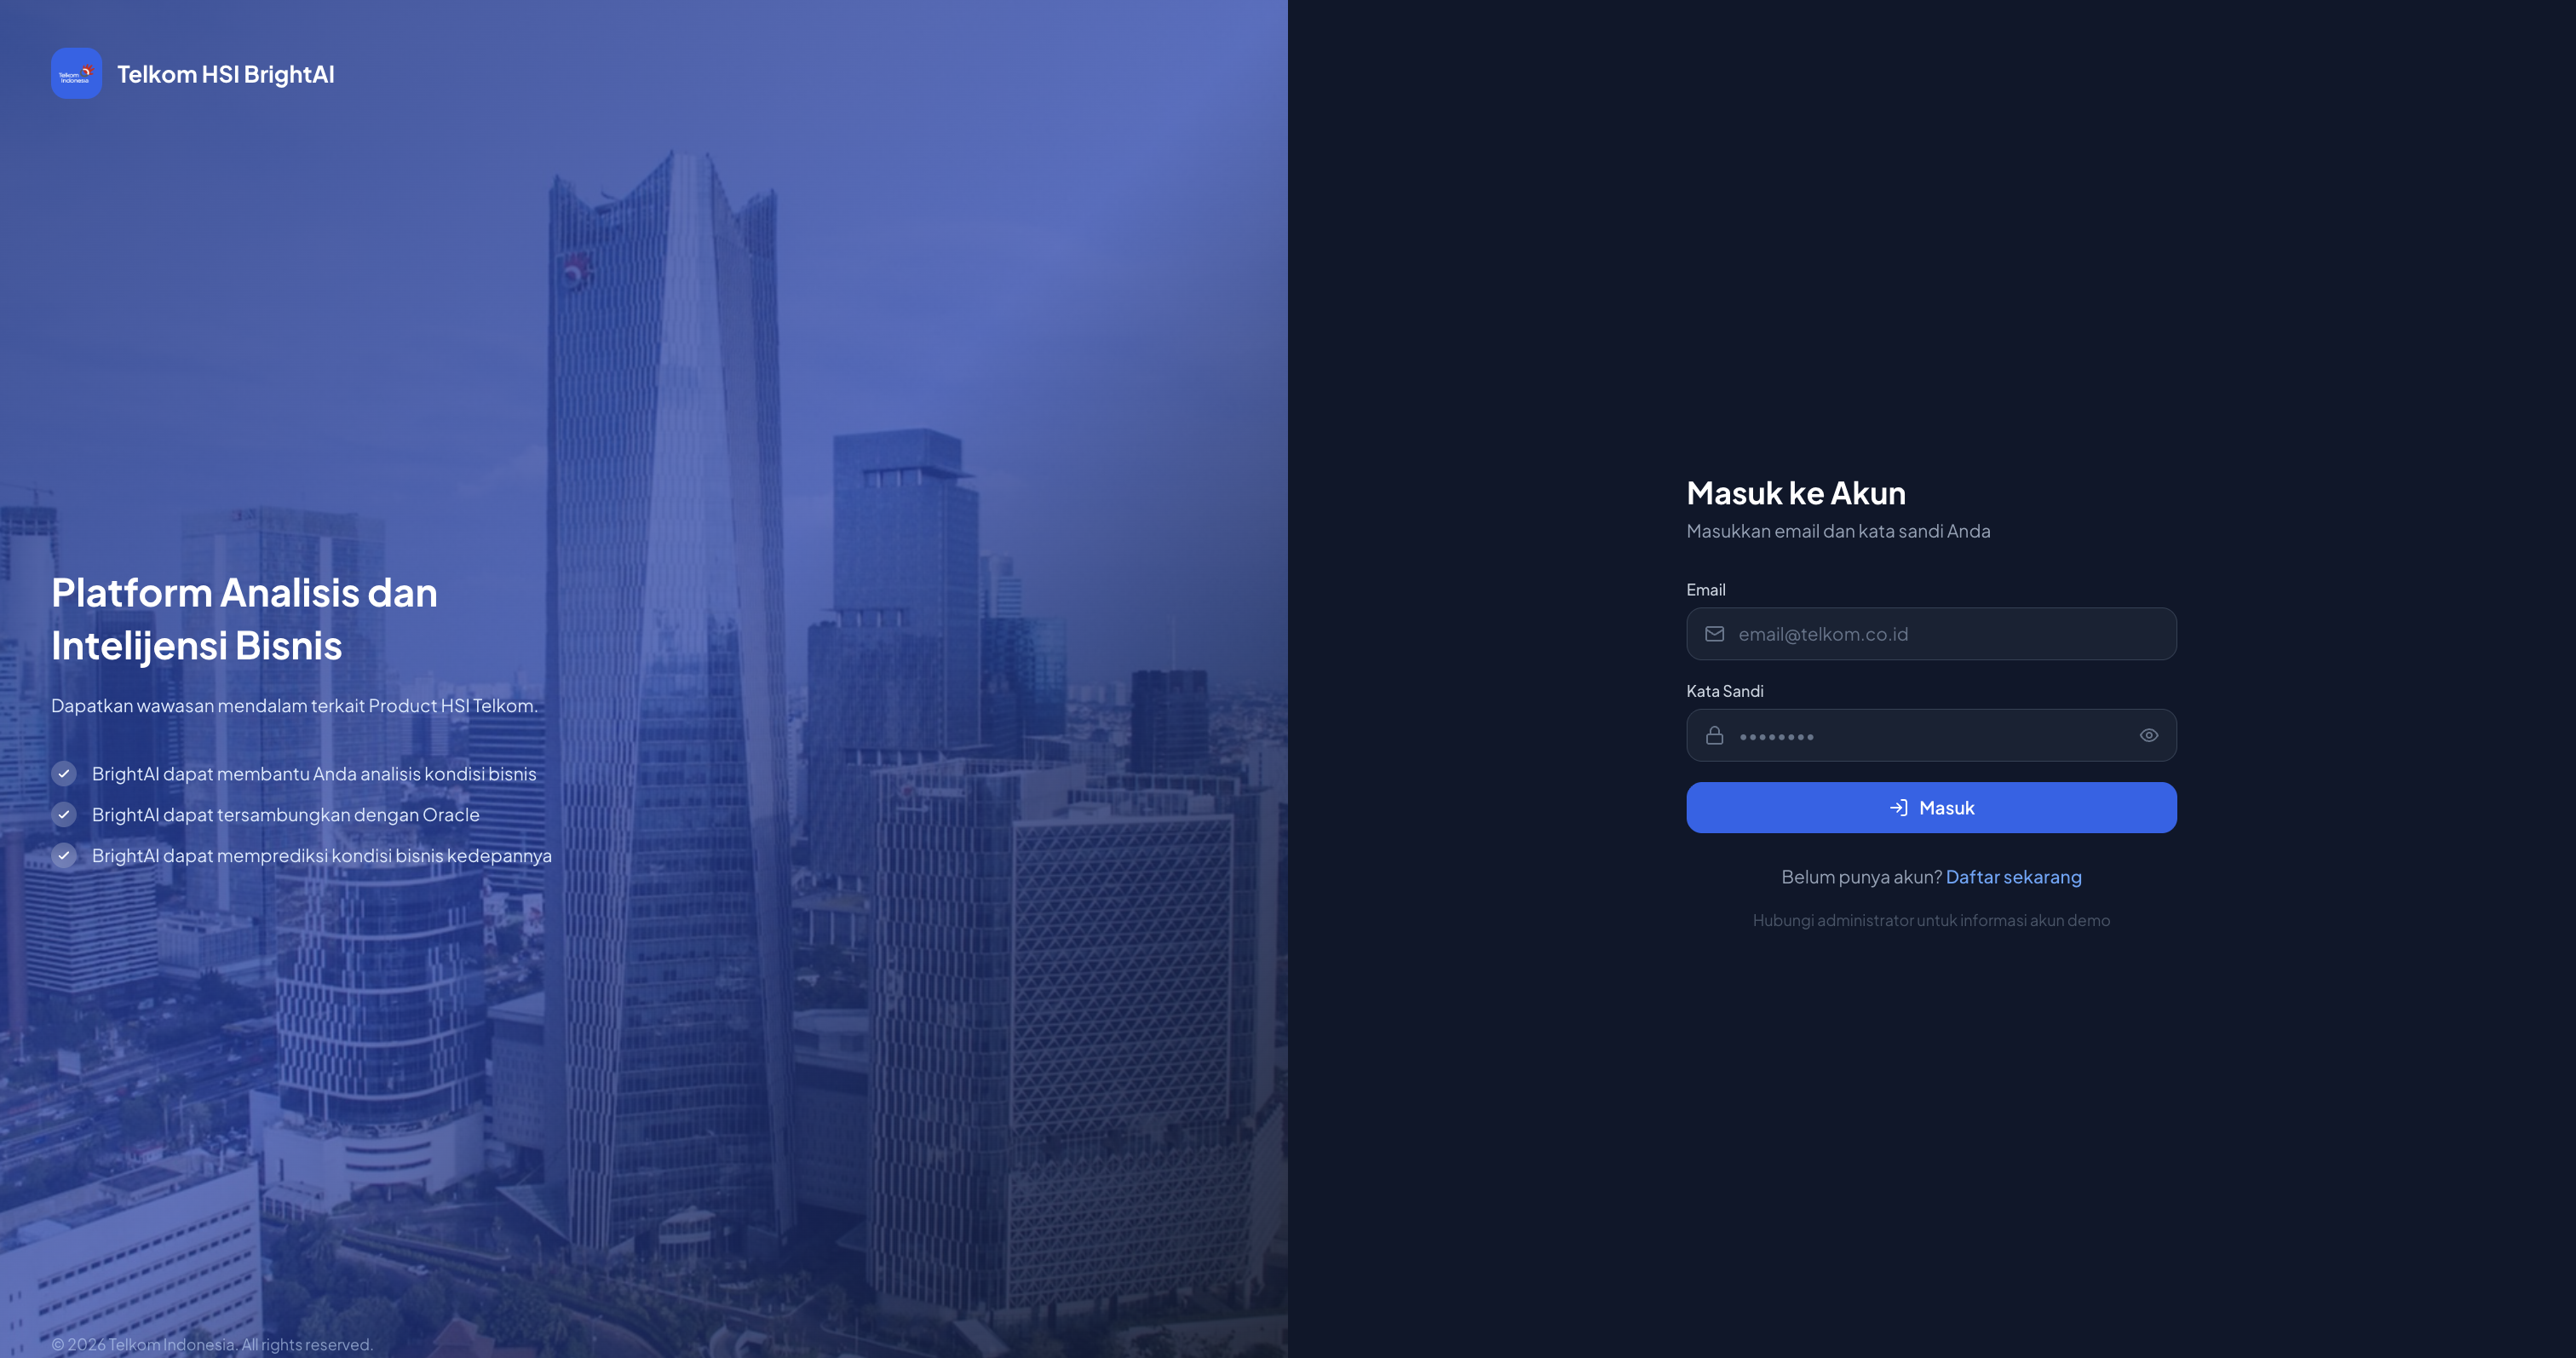
\includegraphics[width=0.85\textwidth]{images/imagemockup1}
\caption{Halaman Masuk (\textit{Login}) Sistem BrightAI}
\label{fig:ui-login}
\end{figure}

\subsubsection{Halaman Registrasi}

Halaman registrasi memungkinkan pengguna internal baru untuk membuat akun pada sistem BrightAI. Formulir registrasi meminta empat isian, yaitu \textit{username}, alamat surel, nama lengkap, dan kata sandi dengan persyaratan minimal enam karakter yang terdiri dari kombinasi huruf besar, huruf kecil, dan angka. Halaman ini dapat diakses melalui tautan ``Daftar sekarang'' pada halaman masuk, dan sebaliknya pengguna yang telah memiliki akun dapat kembali ke halaman masuk melalui tautan ``Masuk''. Gambar~\ref{fig:ui-register} menunjukkan tampilan halaman registrasi.

\begin{figure}[h]
\centering
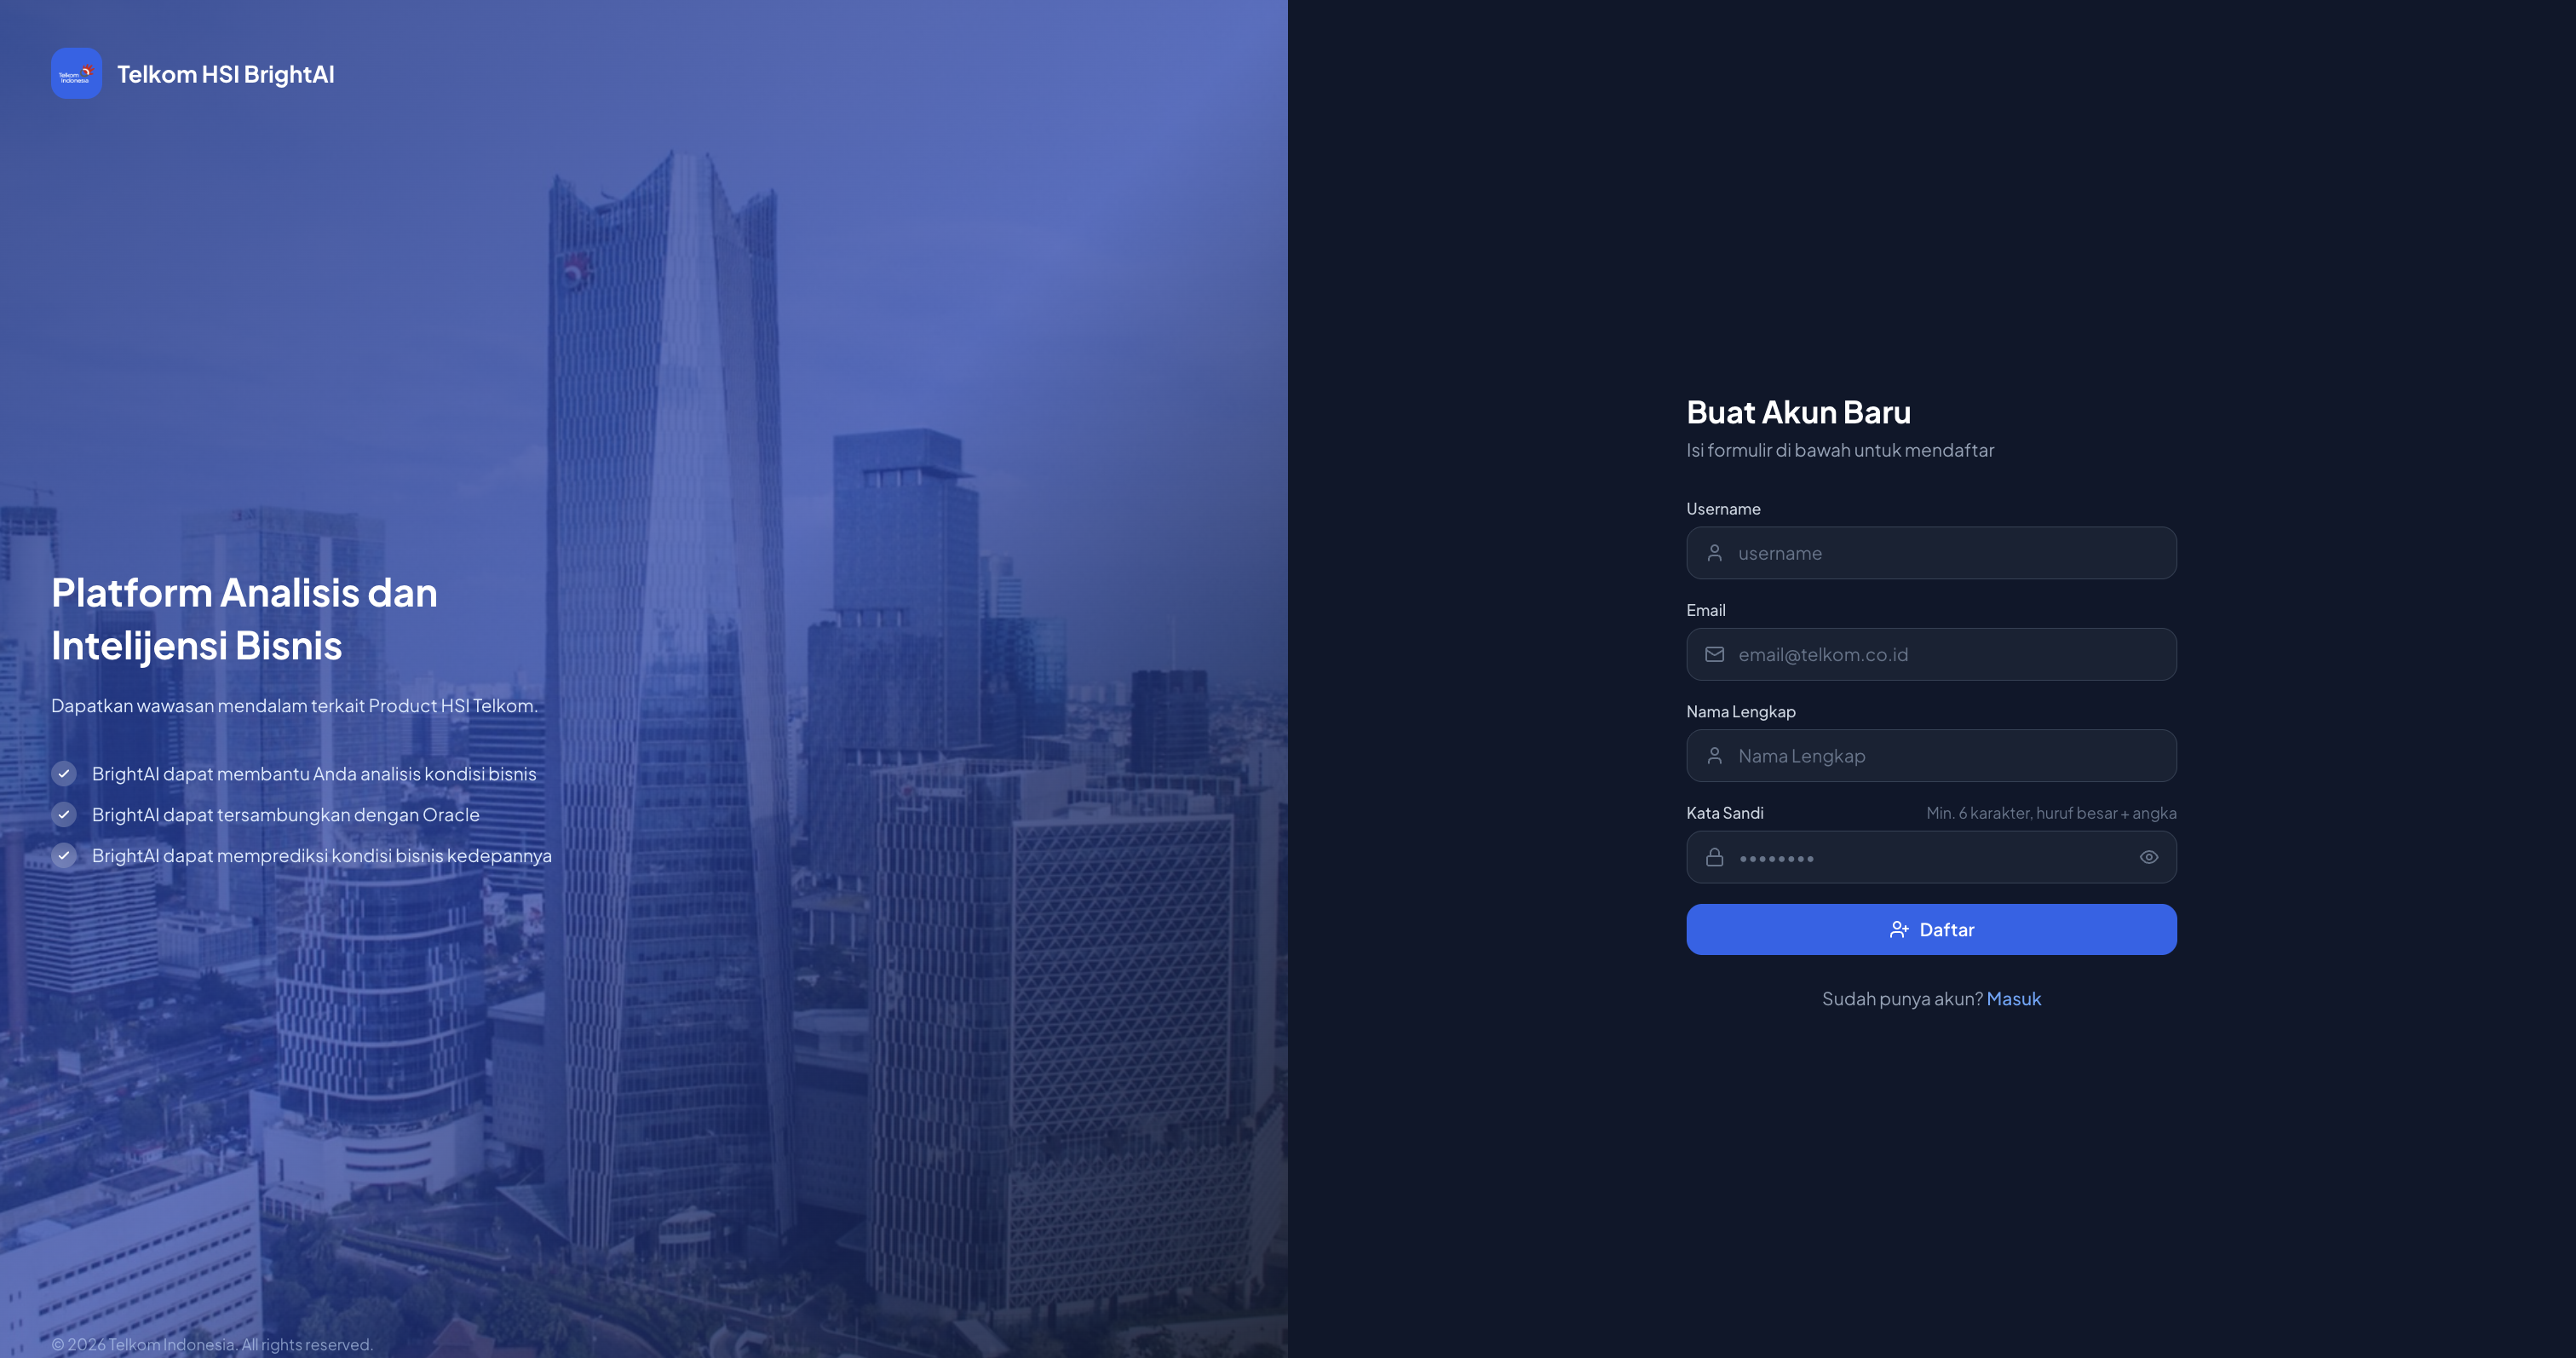
\includegraphics[width=0.85\textwidth]{images/imagemockup2}
\caption{Halaman Registrasi Pengguna Baru}
\label{fig:ui-register}
\end{figure}

\subsubsection{Halaman Utama \textit{Chatbot}}

Halaman utama \textit{chatbot} merupakan antarmuka inti sistem yang terdiri dari tiga area: (1)~bilah navigasi vertikal di sisi kiri yang menyediakan akses ke modul \textit{chatbot}, profil, dan pengaturan; (2)~panel riwayat percakapan yang memungkinkan pengguna mengelola sesi percakapan, termasuk pencarian, penggantian nama, penyematan (\textit{pin}), dan penghapusan sesi; serta (3)~area percakapan utama yang menampilkan pesan pengguna dan respons sistem. Di bagian bawah, alur terpandu (\textit{guided flow}) menyediakan mekanisme interaksi terstruktur melalui pemilihan jenis analisis, kategori domain, dan pertanyaan yang telah dikurasi. Bilah tajuk di bagian atas menampilkan status koneksi server, pengalih tema, dan informasi pengguna. Gambar~\ref{fig:ui-chat} menunjukkan tampilan halaman utama \textit{chatbot}.

\begin{figure}[h]
\centering
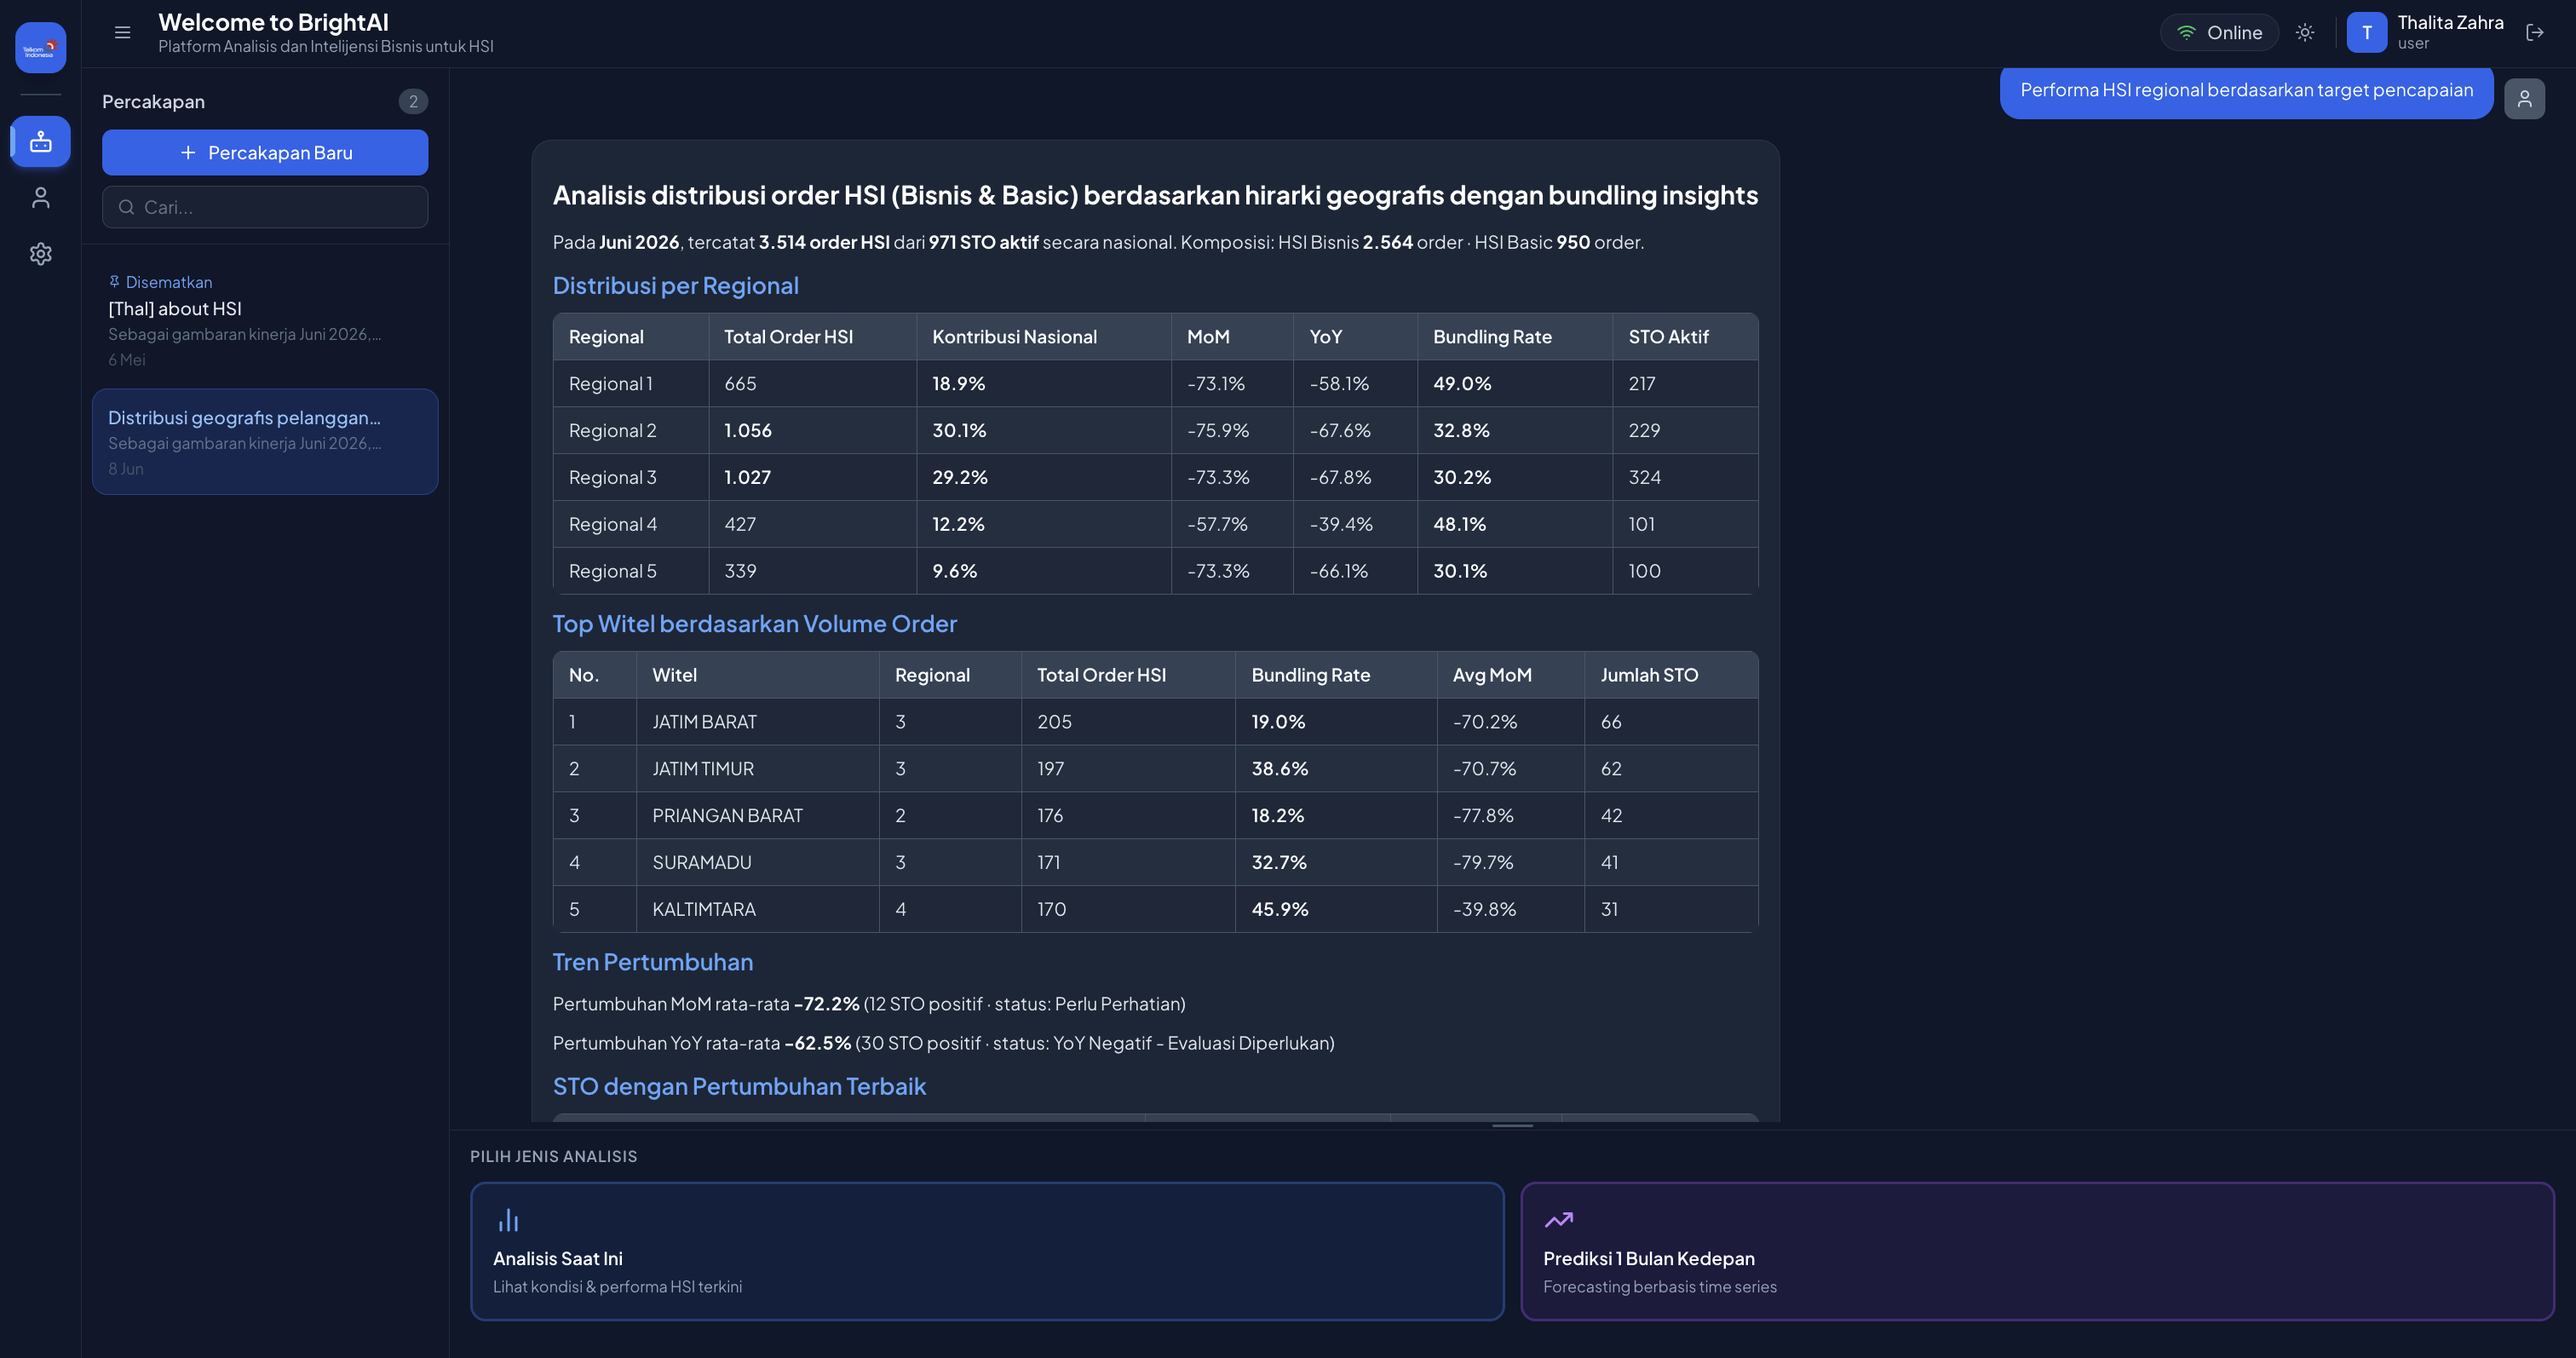
\includegraphics[width=0.85\textwidth]{images/imagemockup3}
\caption{Halaman Utama \textit{Chatbot} BrightAI}
\label{fig:ui-chat}
\end{figure}

\subsubsection{Halaman Profil}

Halaman profil menampilkan informasi akun pengguna yang sedang masuk, meliputi nama lengkap, \textit{username}, alamat surel, dan peran (\textit{role}) dalam sistem. Halaman ini dapat diakses melalui ikon pengguna pada bilah navigasi vertikal. Gambar~\ref{fig:ui-profile} menunjukkan tampilan halaman profil.

\begin{figure}[h]
\centering
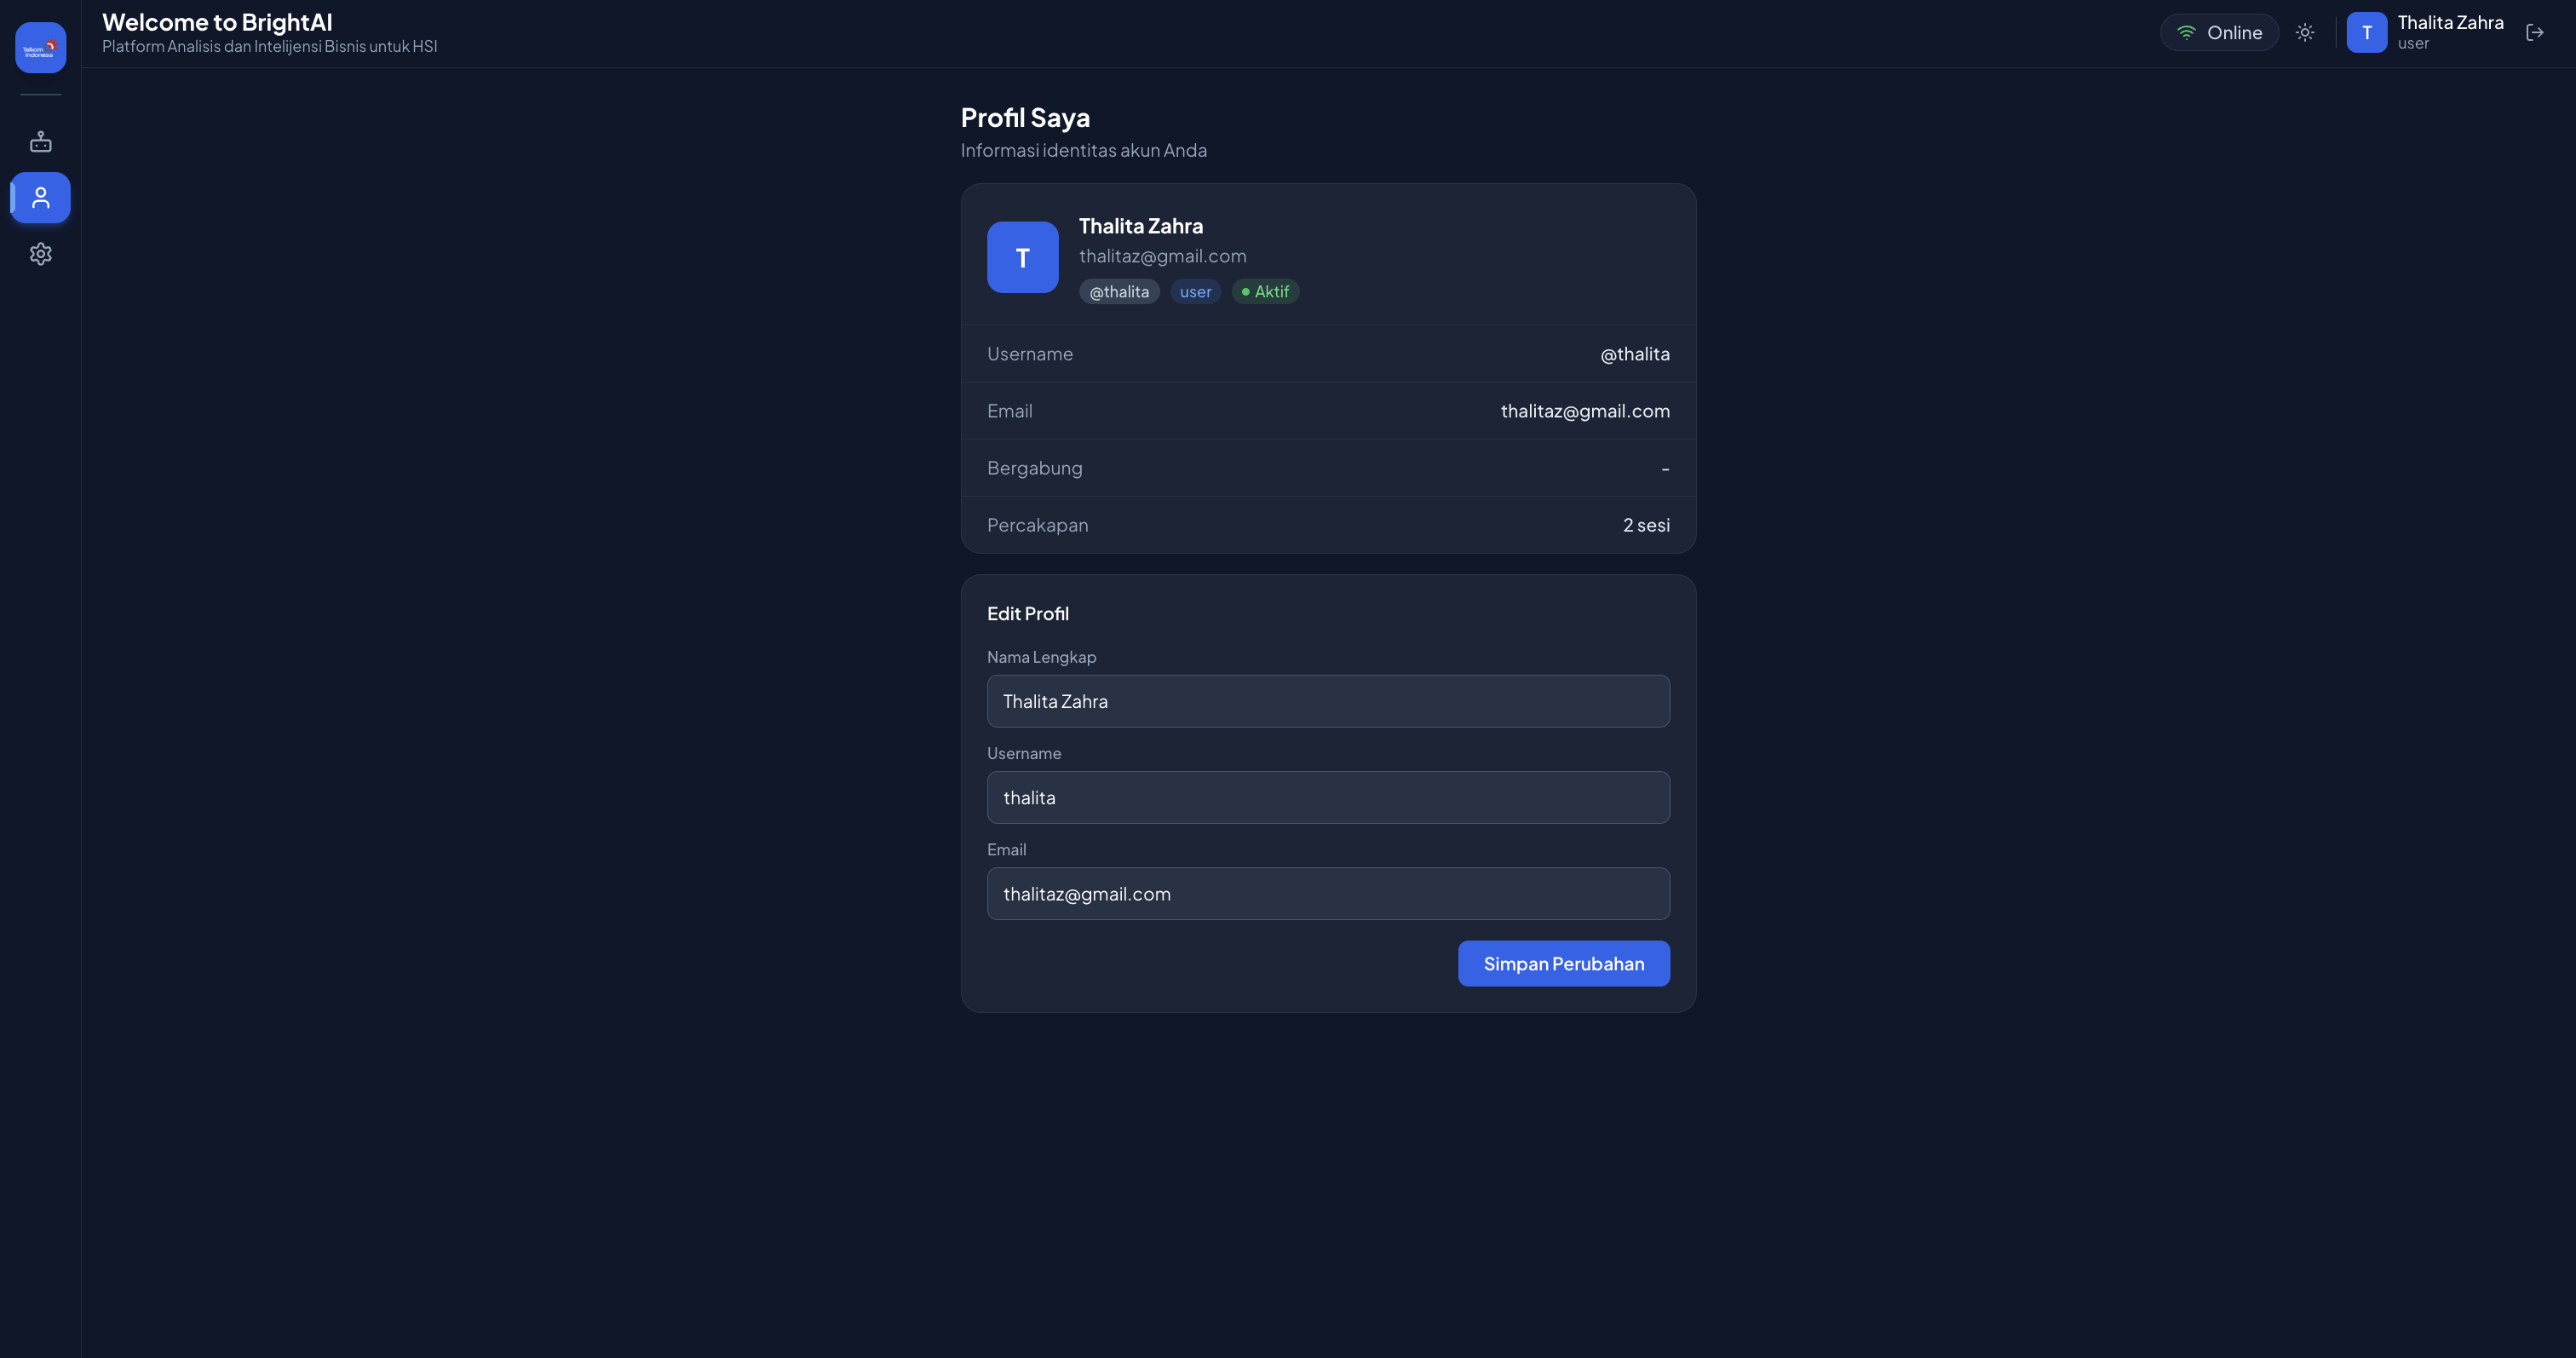
\includegraphics[width=0.85\textwidth]{images/imagemockup4}
\caption{Halaman Profil Pengguna}
\label{fig:ui-profile}
\end{figure}

\subsubsection{Halaman Pengaturan}

Halaman pengaturan menyediakan opsi konfigurasi antarmuka bagi pengguna, termasuk pengalihan tema tampilan dan preferensi notifikasi. Halaman ini dapat diakses melalui ikon pengaturan pada bilah navigasi vertikal. Gambar~\ref{fig:ui-settings} menunjukkan tampilan halaman pengaturan.

\begin{figure}[h]
\centering
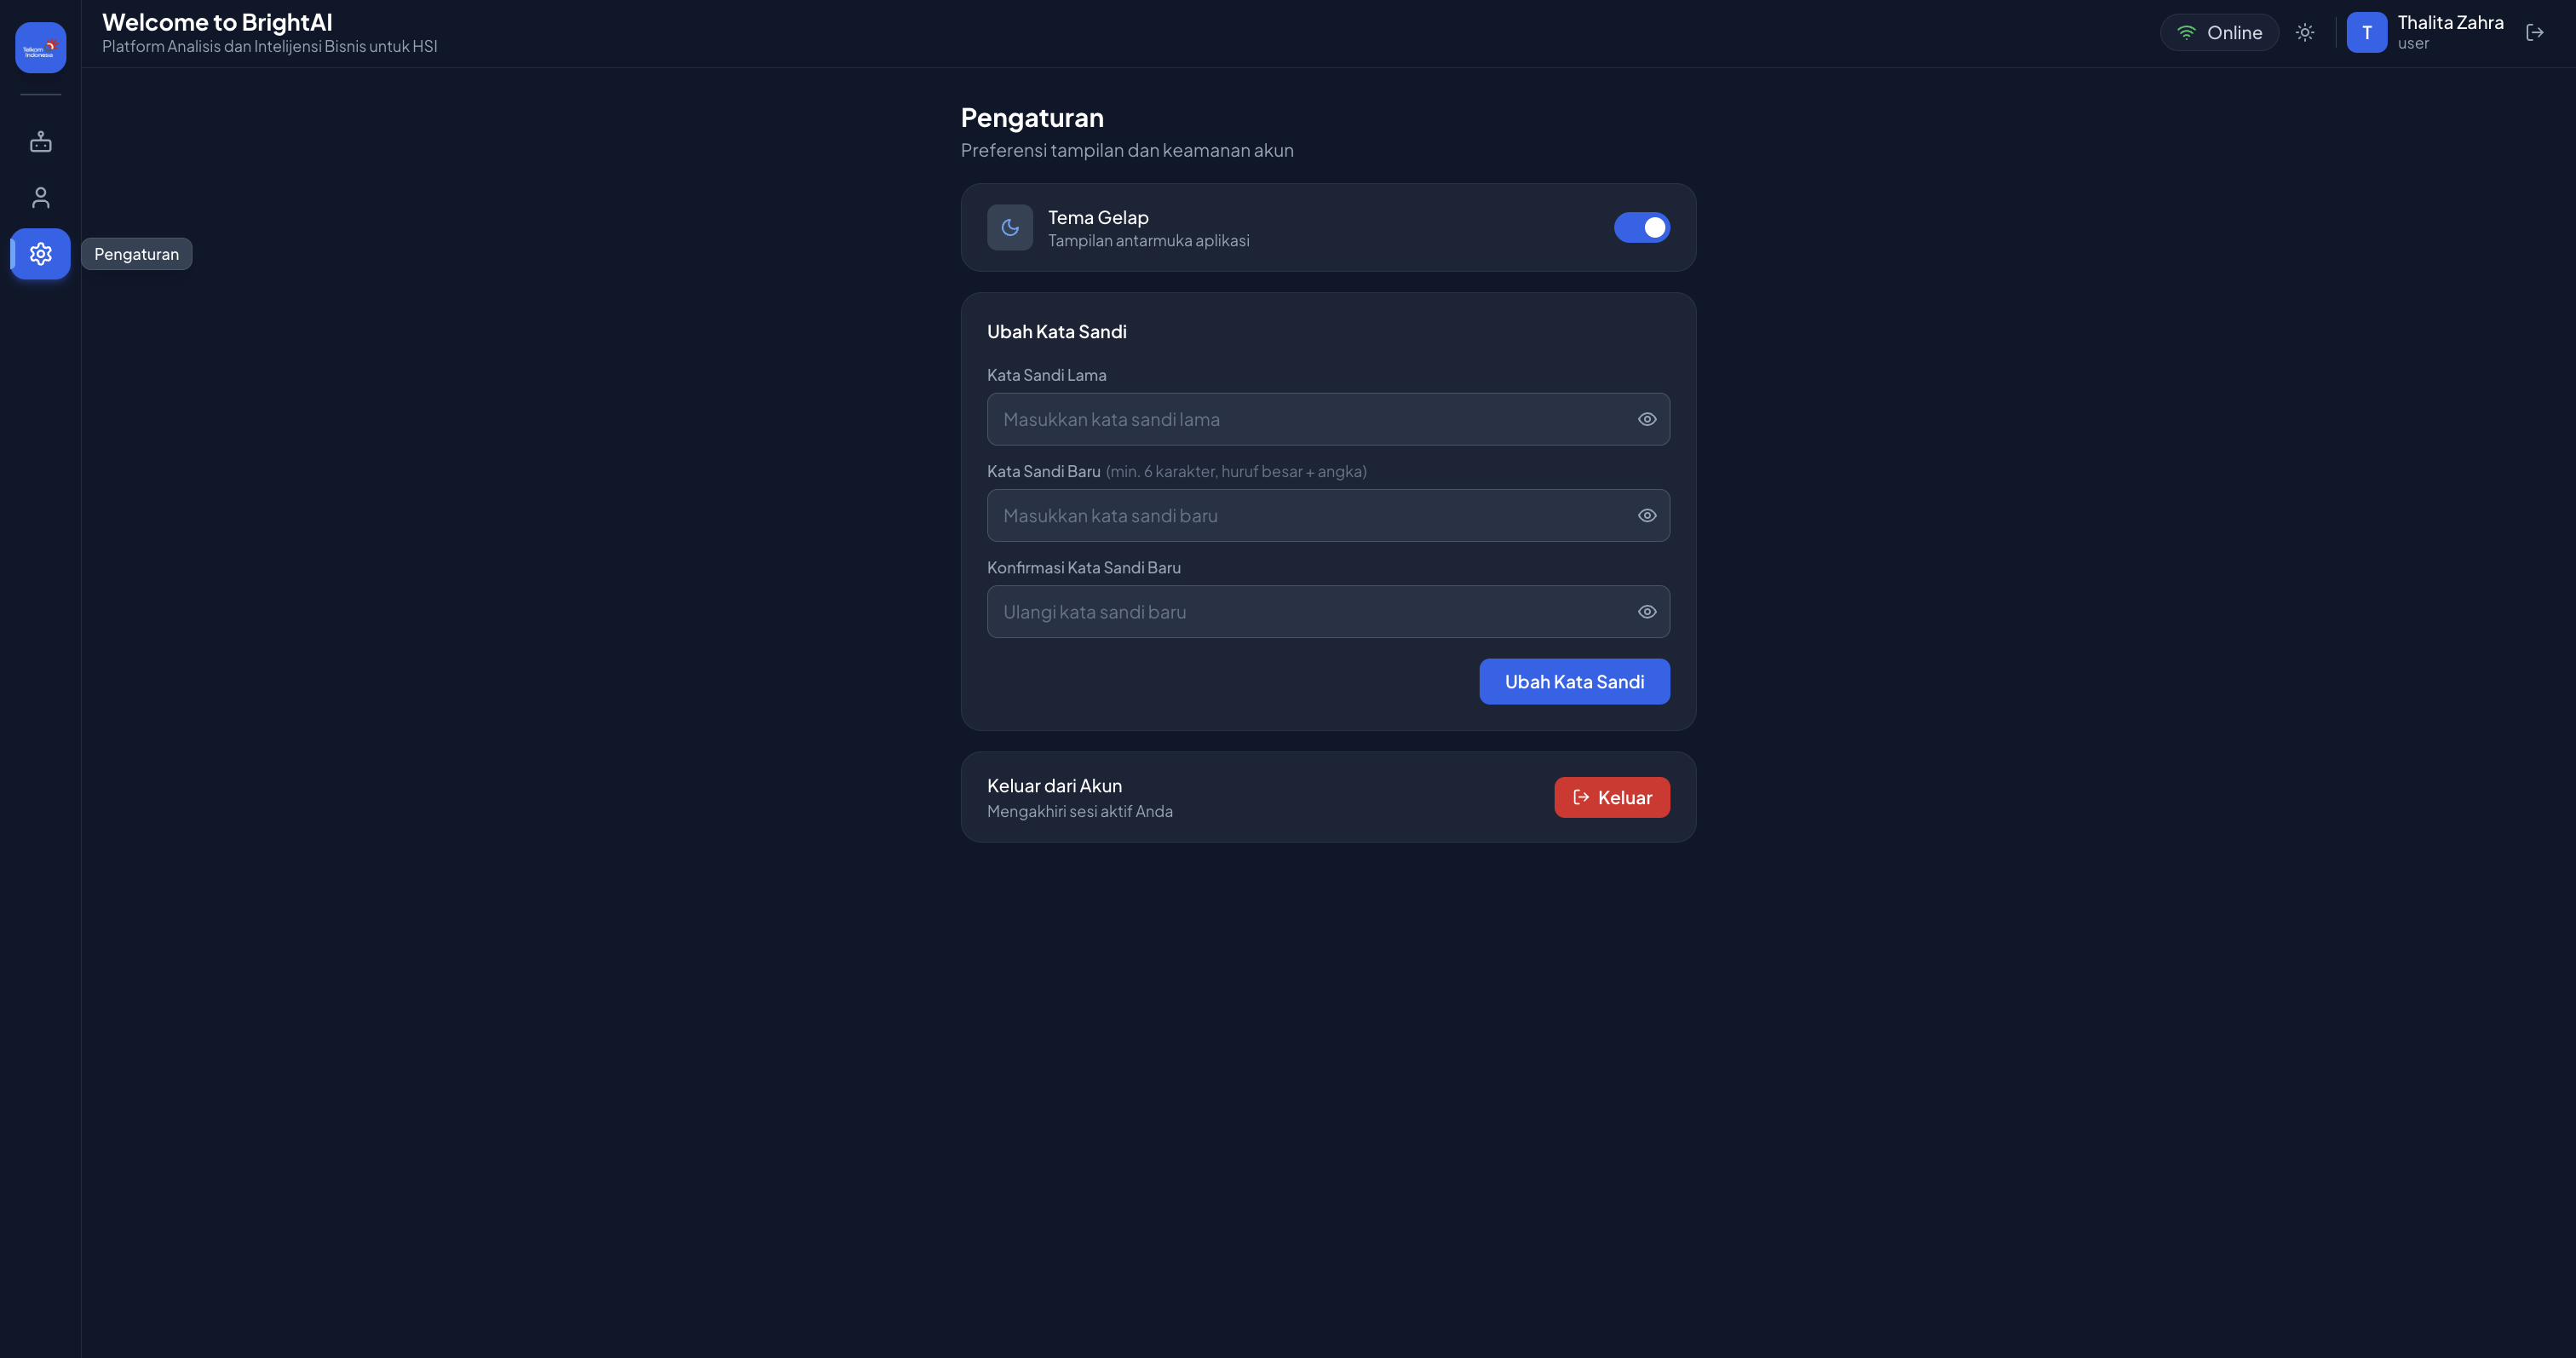
\includegraphics[width=0.85\textwidth]{images/imagemockup5}
\caption{Halaman Pengaturan Sistem}
\label{fig:ui-settings}
\end{figure}

\subsubsection{Tampilan Tema Terang (\textit{Light Mode})}

Sistem mendukung dua tema tampilan, yaitu tema gelap (\textit{dark mode}) sebagai tema bawaan dan tema terang (\textit{light mode}). Pengguna dapat beralih antara kedua tema melalui tombol pengalih pada bilah tajuk. Seluruh komponen antarmuka, termasuk area percakapan, panel riwayat, dan alur terpandu, menyesuaikan skema warna secara konsisten sesuai tema yang dipilih. Gambar~\ref{fig:ui-light} menunjukkan tampilan sistem dalam tema terang.

\begin{figure}[h]
\centering
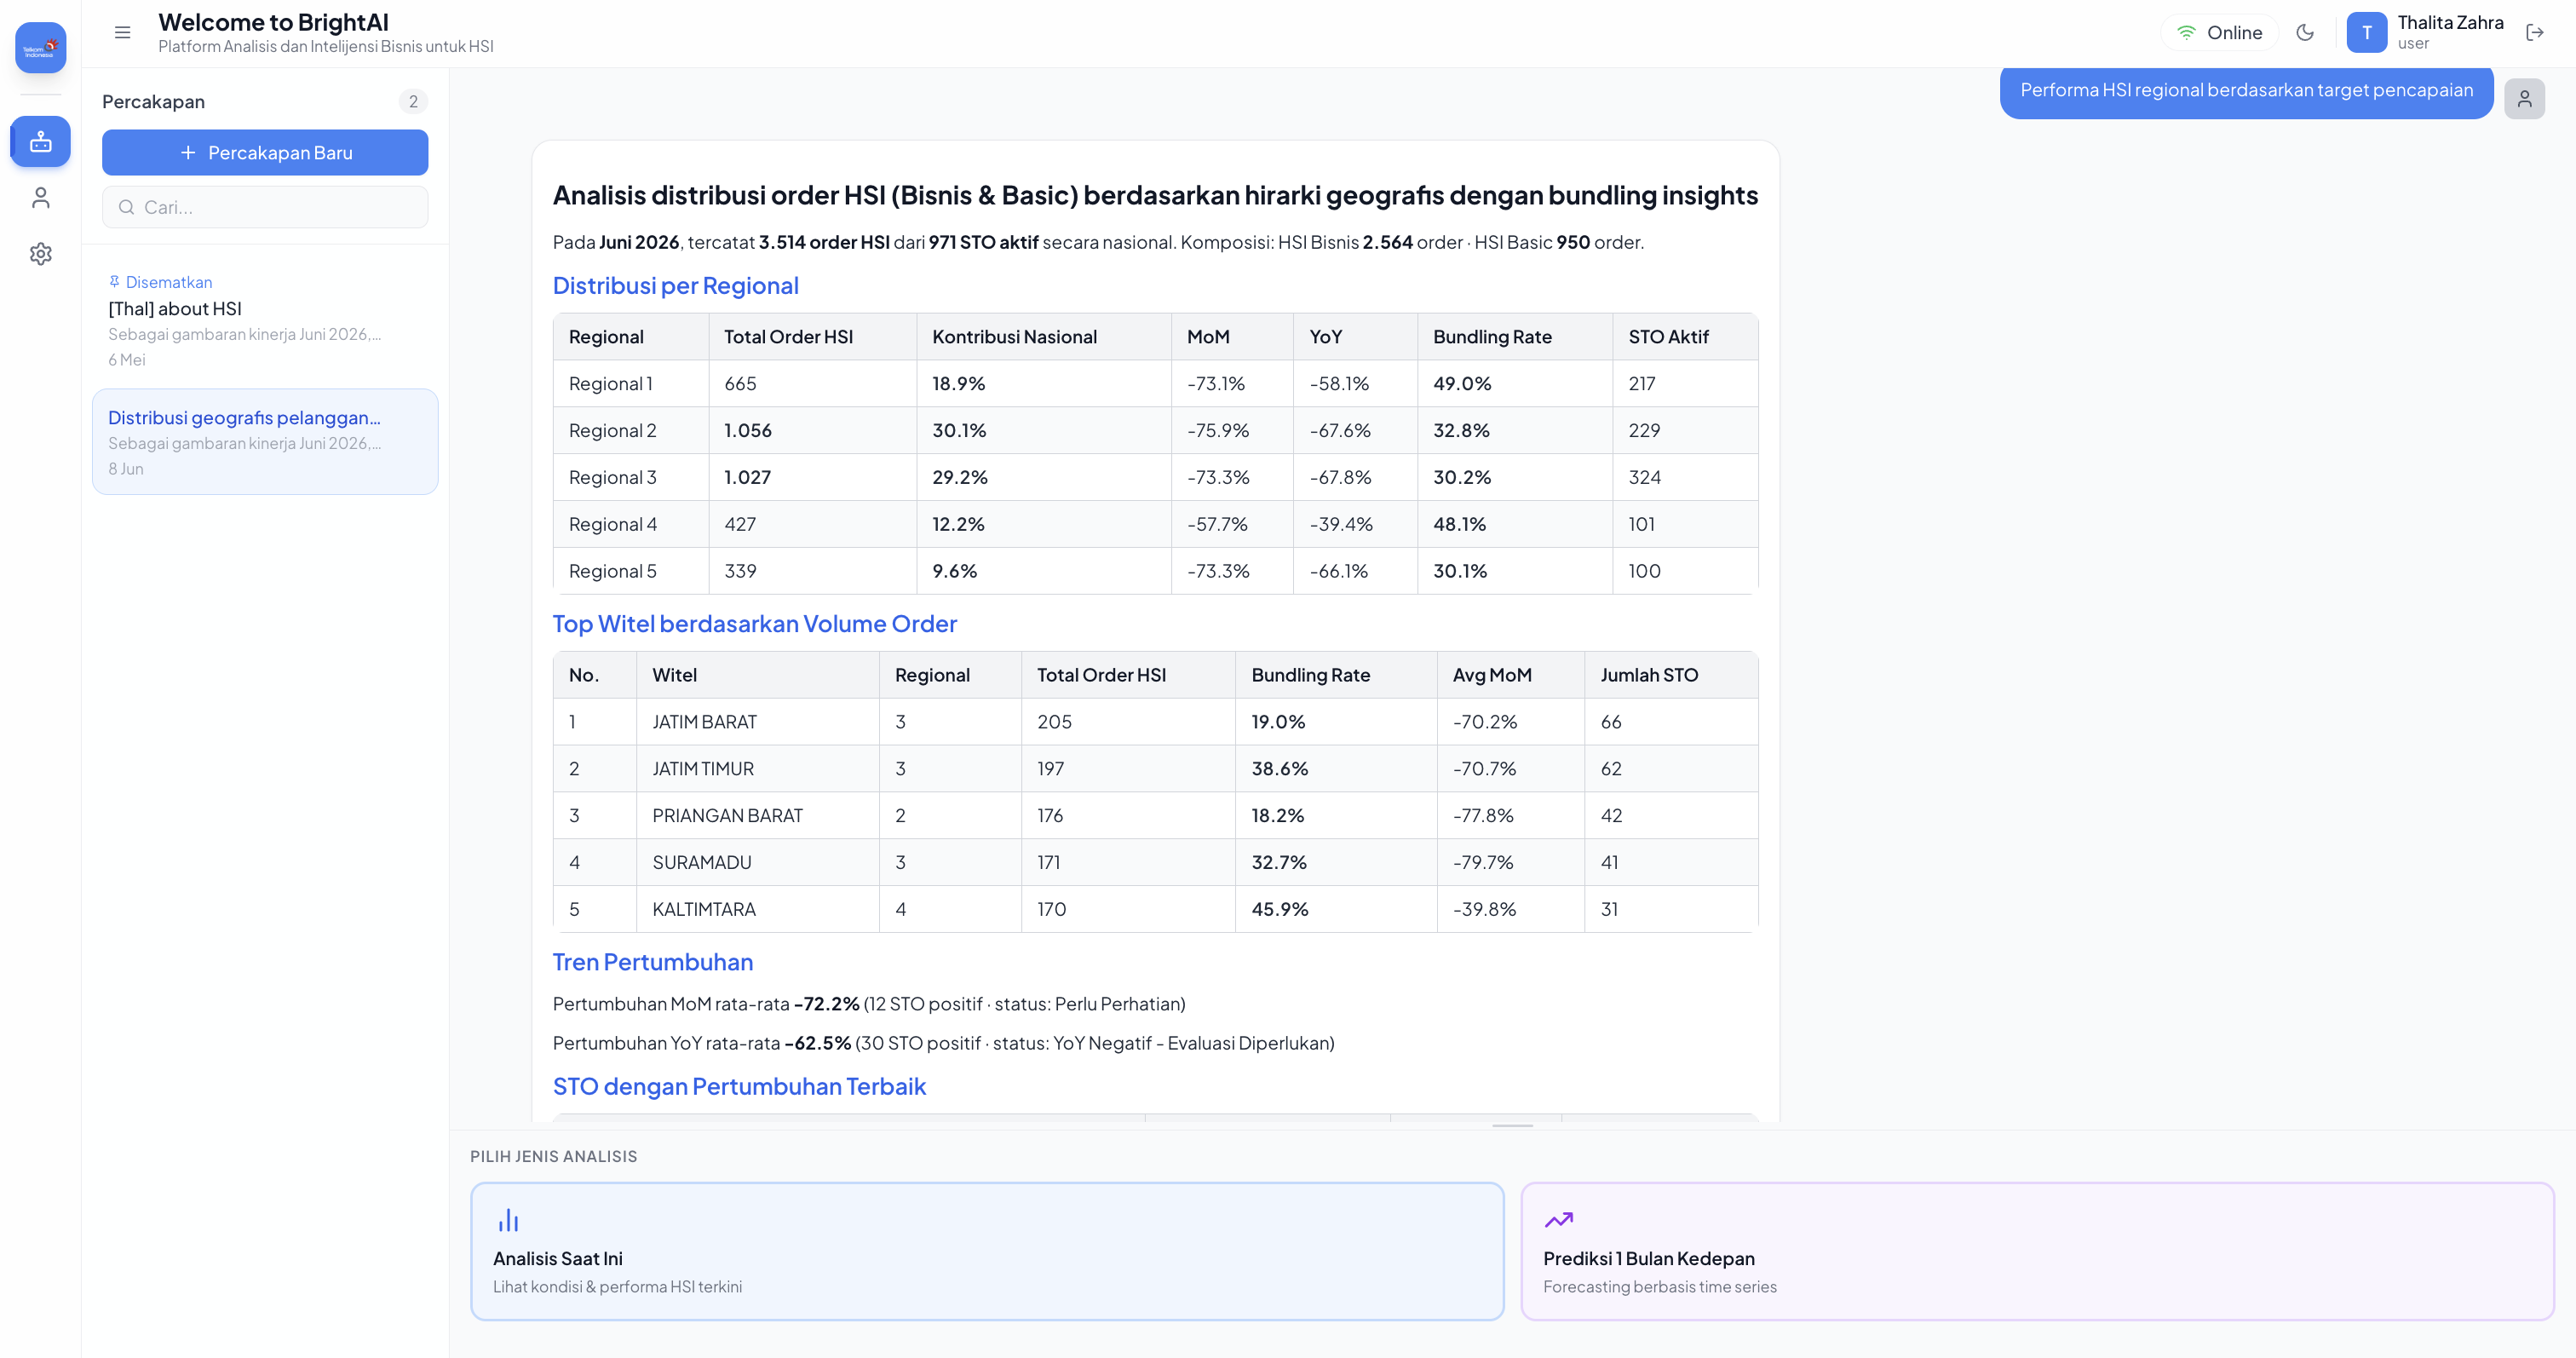
\includegraphics[width=0.85\textwidth]{images/imagemockup6}
\caption{Tampilan Antarmuka \textit{Chatbot} dalam Tema Terang (\textit{Light Mode})}
\label{fig:ui-light}
\end{figure}

\subsubsection{Detail Respons \textit{Rule-Based Query}}

Ketika pengguna mengajukan pertanyaan analitik melalui antarmuka percakapan, sistem mencocokkan kueri tersebut dengan salah satu dari 38 aturan bisnis yang tersedia, mengeksekusi kueri SQL terhadap \textit{Enterprise Data Warehouse}, dan menghasilkan respons naratif dalam bahasa Indonesia menggunakan modul NLG berbasis templat. Respons ditampilkan dalam format \textit{Markdown} yang mencakup judul analisis, tabel data dengan angka terformat sesuai konvensi Indonesia, poin-poin wawasan bisnis, serta metadata sumber data dan waktu pemrosesan. Gambar~\ref{fig:ui-rulebased} menunjukkan contoh respons sistem terhadap pertanyaan analitik berbasis aturan.

\begin{figure}[h]
\centering
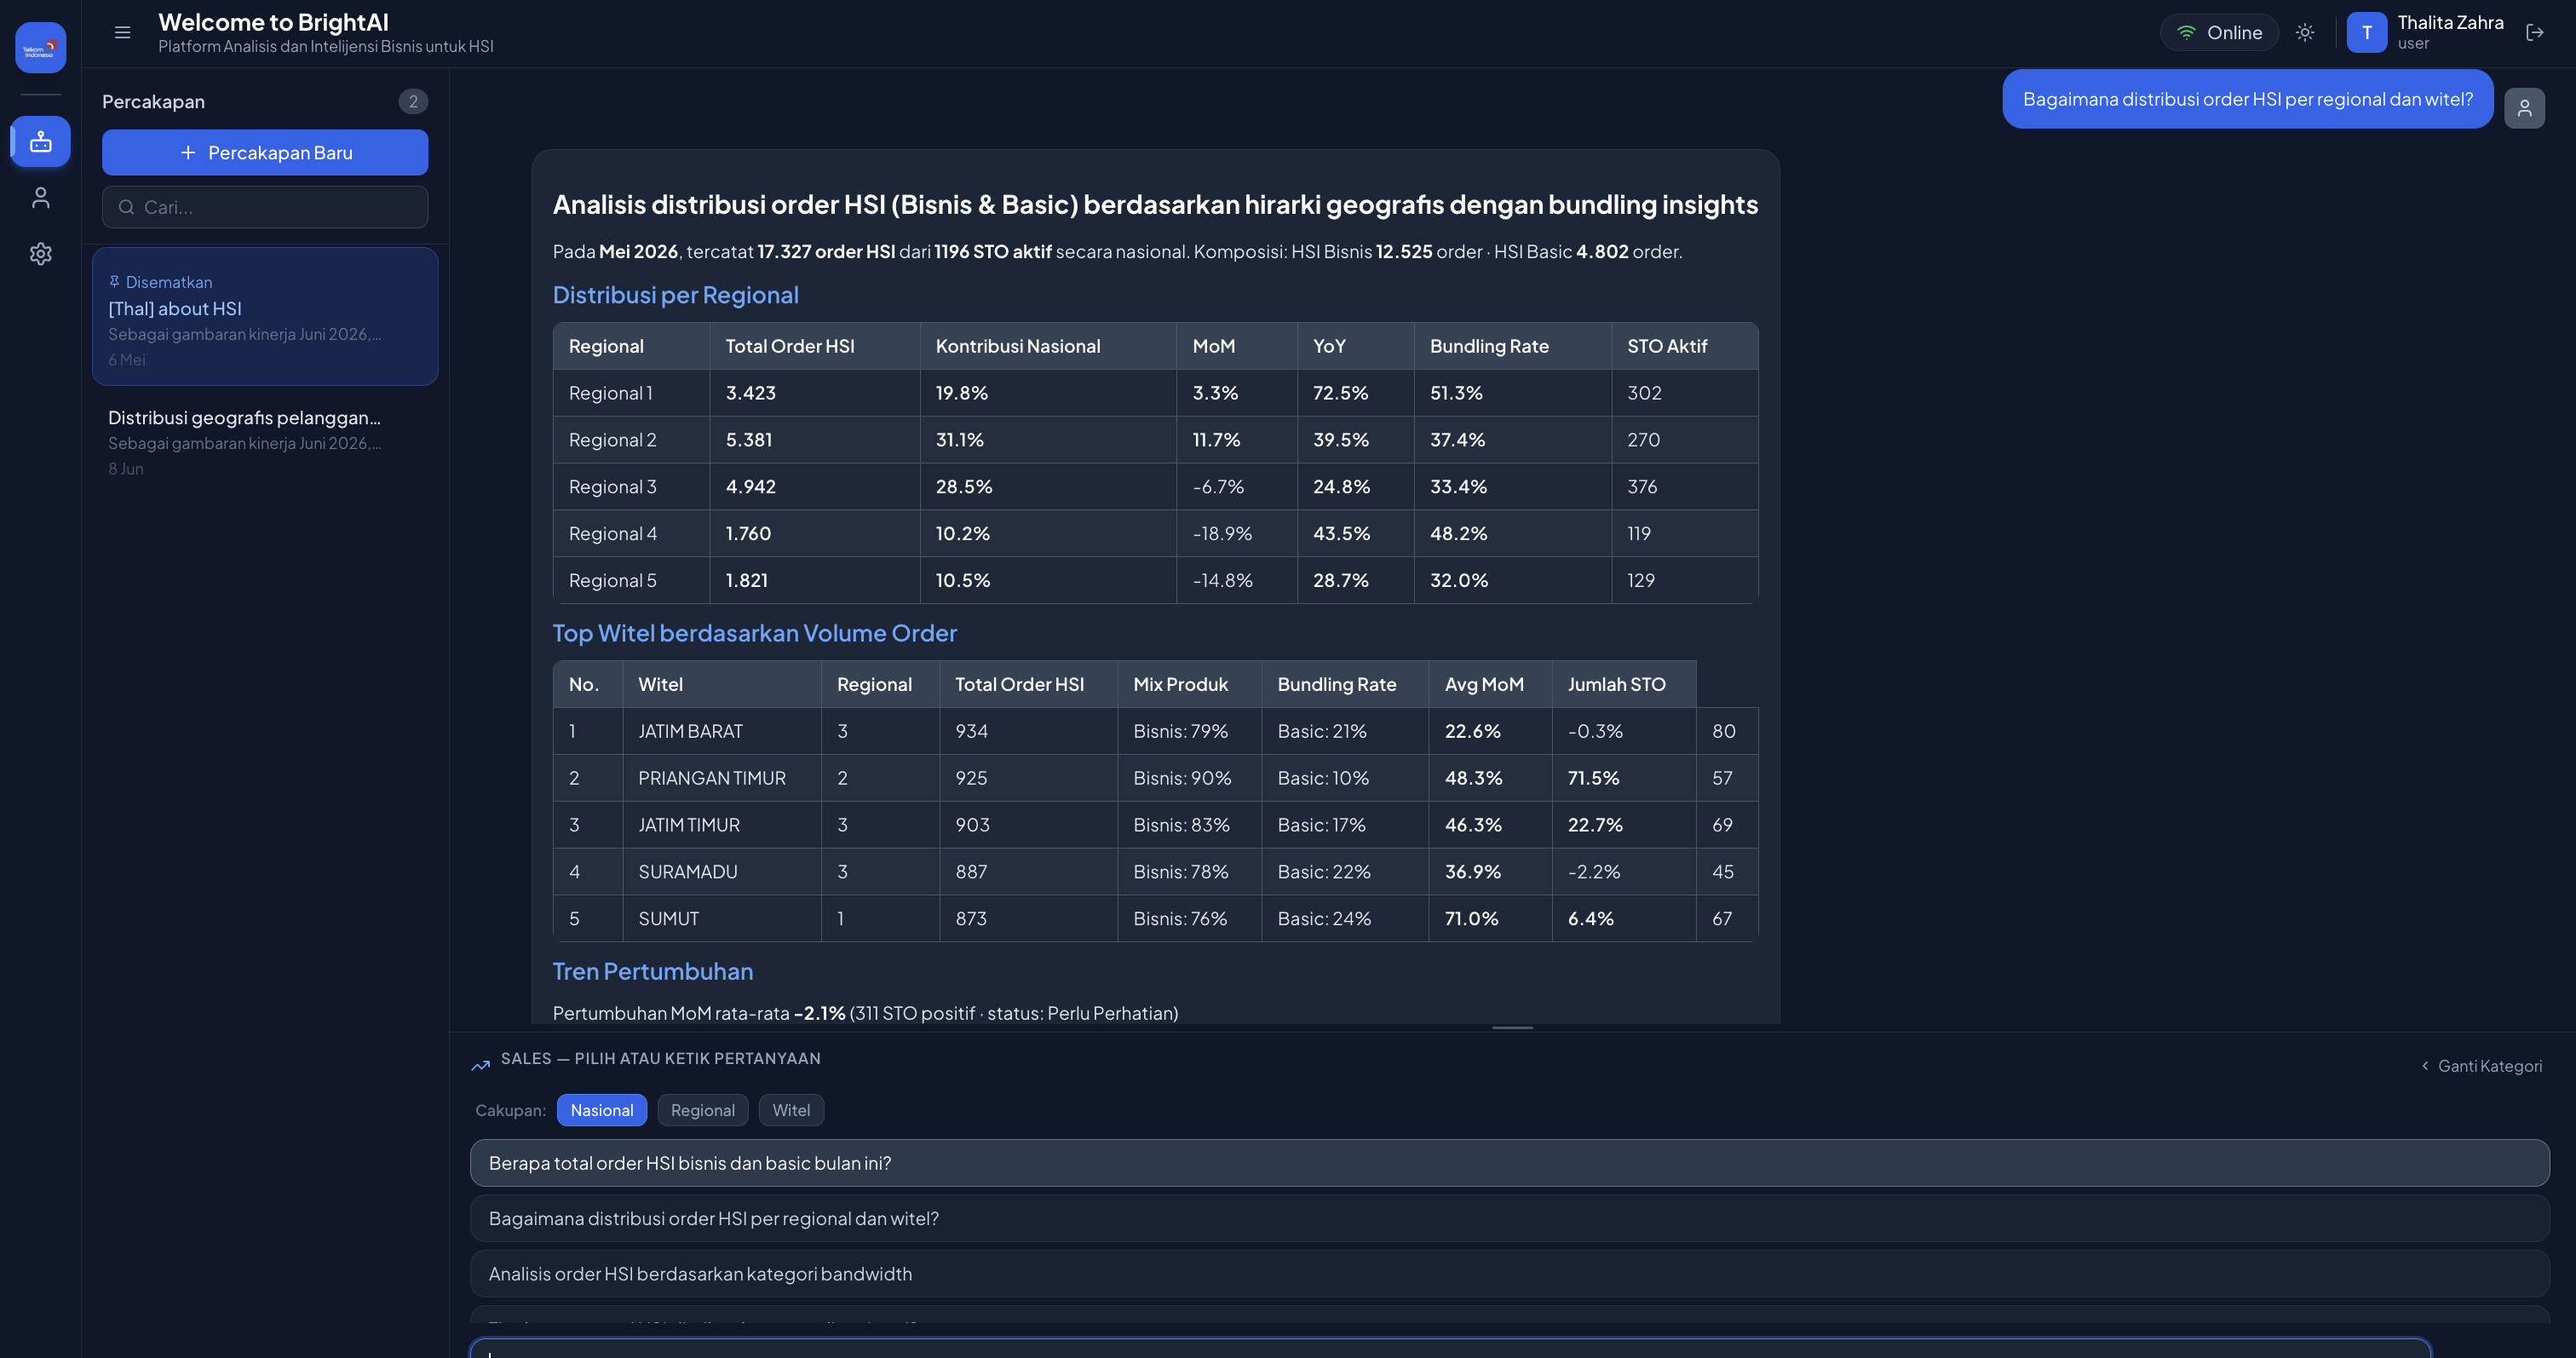
\includegraphics[width=0.85\textwidth]{images/imagemockup7}
\caption{Contoh Respons \textit{Rule-Based Query} dengan Narasi NLG dan Tabel Data}
\label{fig:ui-rulebased}
\end{figure}

\subsubsection{Detail Respons Peramalan Deret Waktu}

Fitur peramalan dapat diakses melalui panel peramalan pada alur terpandu, di mana pengguna memilih metrik yang hendak diramalkan, jenis model (GRU, LSTM, ARIMA, atau \textit{Prophet}), serta cakupan wilayah (nasional, regional, atau \textit{witel}). Hasil peramalan ditampilkan dalam format naratif yang mencakup nilai prediksi untuk periode berikutnya, perbandingan terhadap nilai aktual terakhir, serta metrik evaluasi model (MAE, RMSE, sMAPE, \textit{Skill Score}). Panel ini merupakan realisasi langsung dari tujuan integrasi dan pembandingan model peramalan deret waktu ke dalam antarmuka \textit{chatbot}. Gambar~\ref{fig:ui-forecast} menunjukkan contoh hasil peramalan.

\begin{figure}[h]
\centering
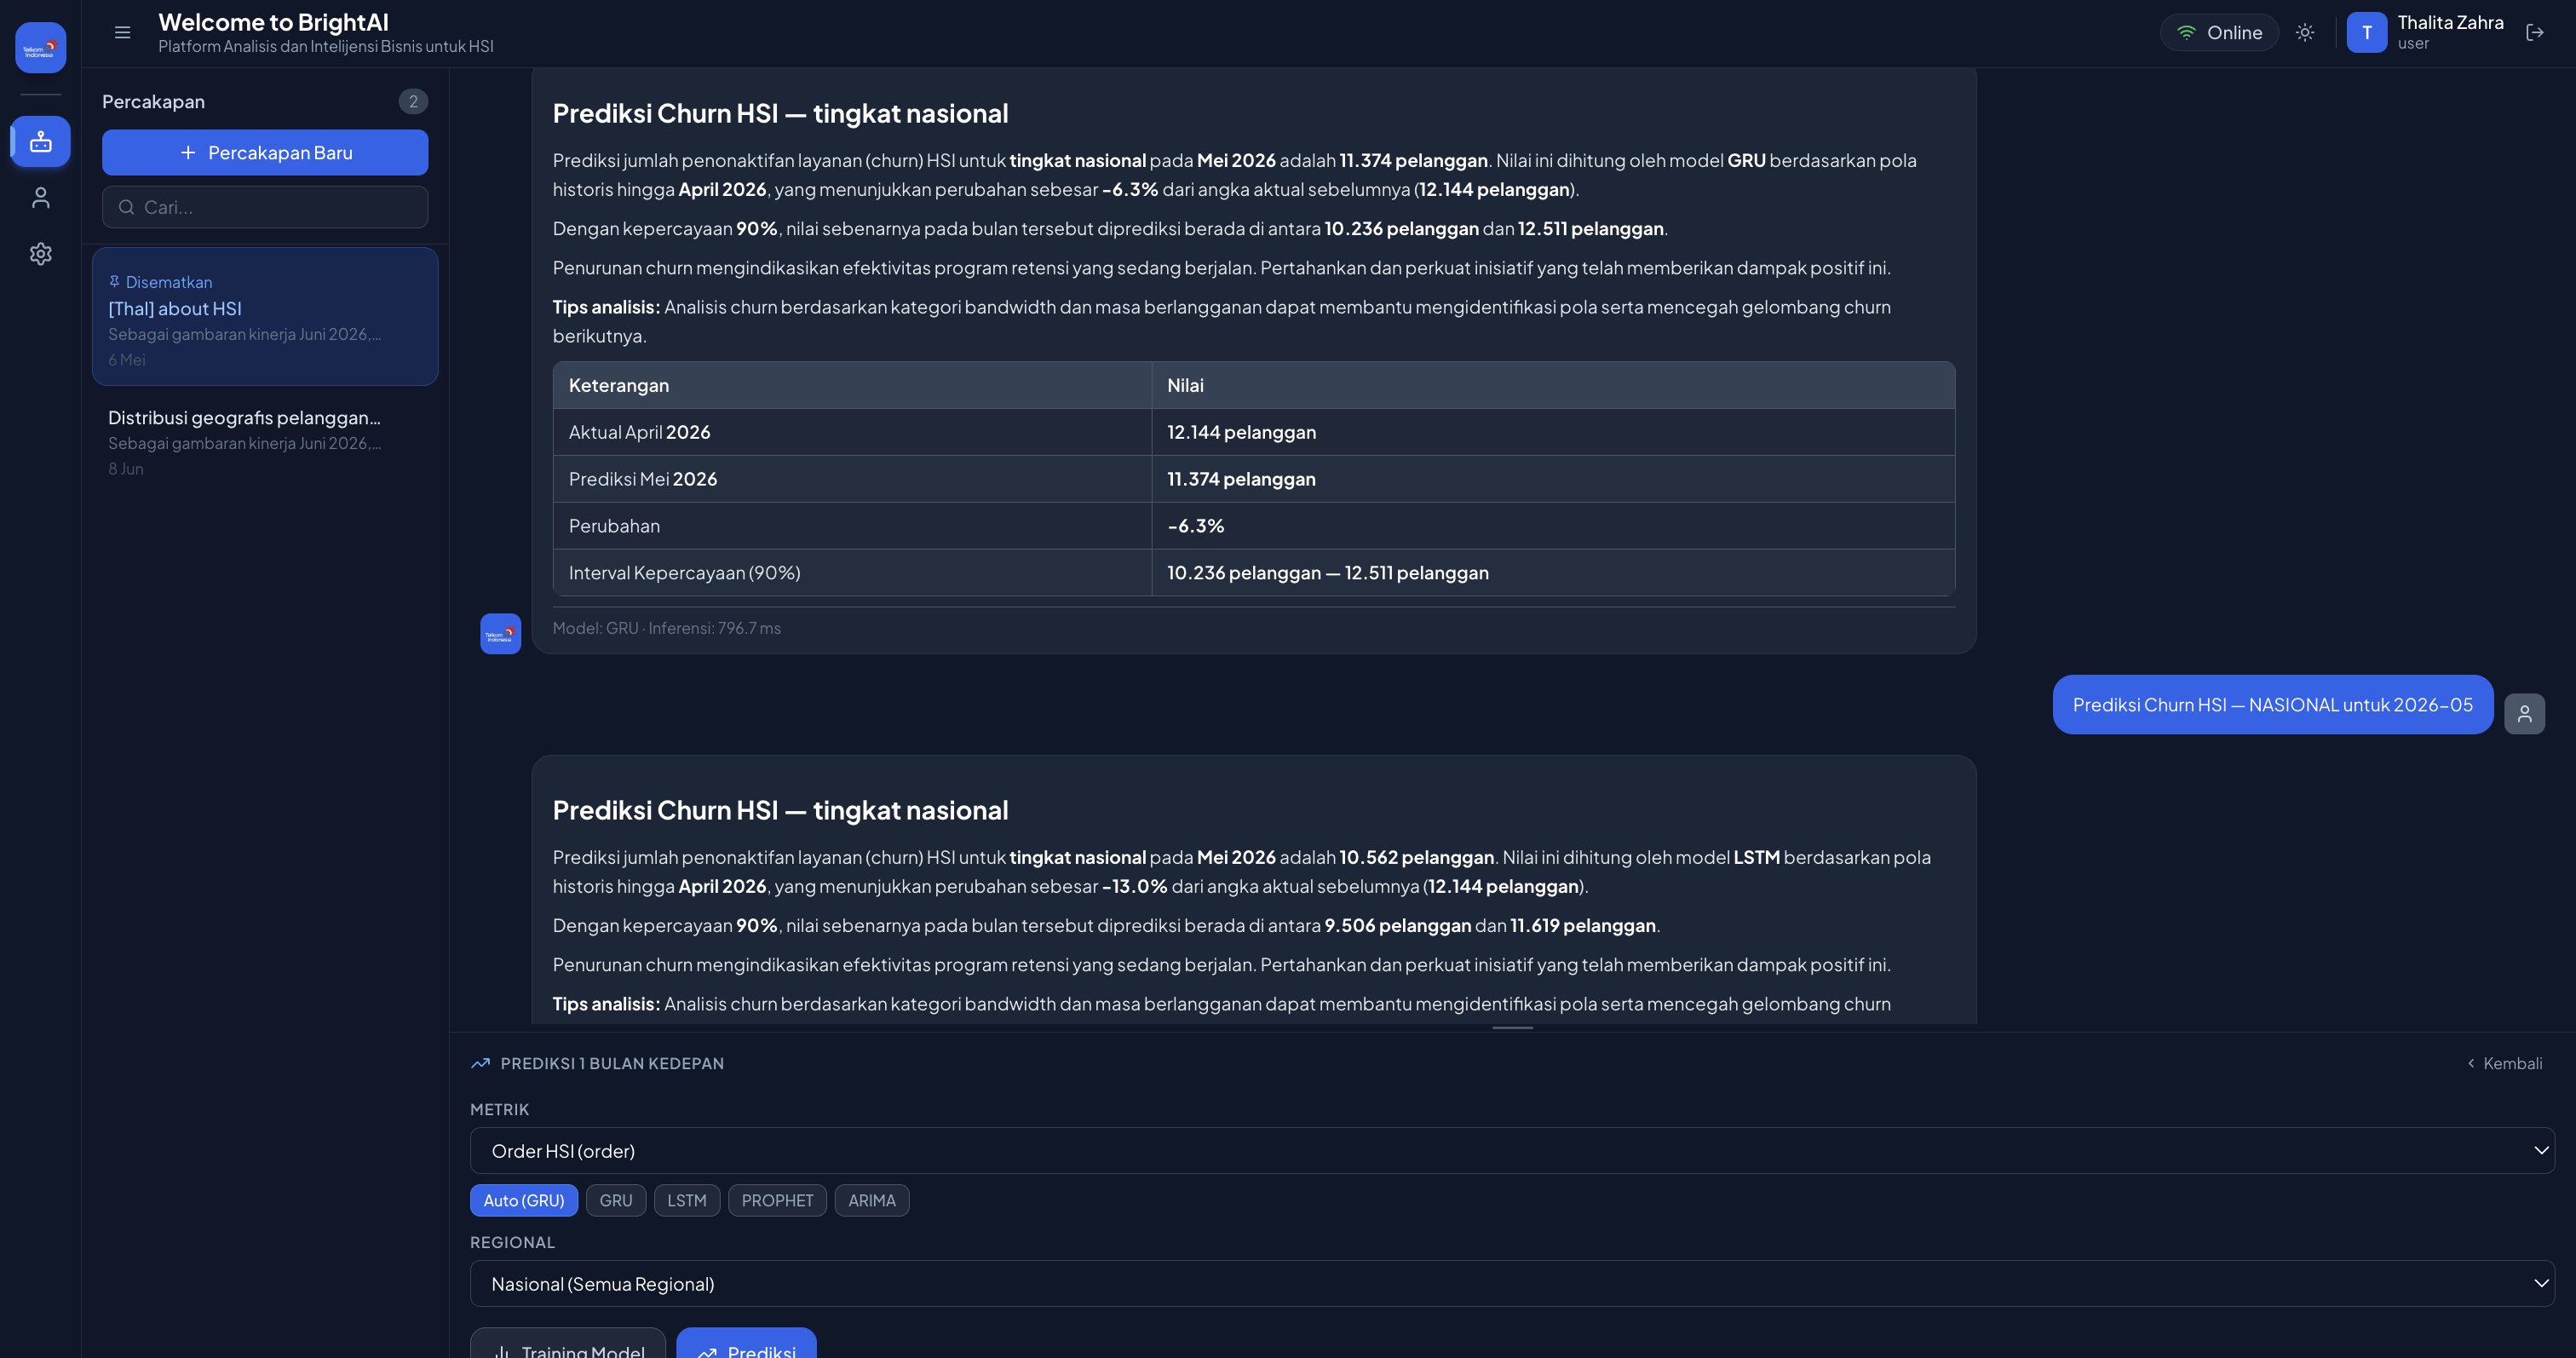
\includegraphics[width=0.85\textwidth]{images/imagemockup8}
\caption{Contoh Hasil Peramalan Deret Waktu melalui Panel \textit{Forecast}}
\label{fig:ui-forecast}
\end{figure}

Sistem terhubung ke Oracle Database melalui dua skema: \texttt{DWH\_MOIS} untuk data analitik dan \texttt{USR\_RPT} untuk data operasional. Sistem menggunakan mekanisme \textit{caching} memori untuk mengoptimalkan waktu respons. Injeksi filter geografis secara dinamis memungkinkan sistem menyajikan analisis pada tingkat nasional, regional, maupun \textit{witel} tanpa duplikasi definisi aturan.

\subsection{Selisih antara Rancangan dan Implementasi}
\label{subsec:selisih-rancangan-implementasi}

Demi transparansi, bagian ini menyatakan secara eksplisit selisih antara komponen yang dirancang pada Bab~\ref{chap:perancangan} dan komponen yang berhasil diimplementasikan. Tabel~\ref{tab:selisih-impl} merangkum selisih tersebut.

\begin{table}[h]
\centering
\caption{Selisih antara Rancangan dan Implementasi}
\label{tab:selisih-impl}
\begin{tabular}{|p{3.5cm}|p{3cm}|p{6cm}|}
\hline
\textbf{Komponen} & \textbf{Status} & \textbf{Keterangan} \\
\hline
\textit{Temporal Fusion Transformer} (TFT) & Tidak diimplementasikan & Dikaji dalam studi literatur (Subbab~\ref{subsec:tft-literatur}) sebagai arsitektur lanjutan, namun tidak termasuk dalam lingkup implementasi penelitian ini karena keterbatasan volume data dan biaya komputasi. TFT tetap menjadi kandidat pengembangan di masa depan. \\
\hline
Model \textit{ensemble} (gabungan keluaran beberapa model) & Tidak diimplementasikan & Dibahas secara teoretis pada kajian literatur, namun implementasi saat ini menjalankan setiap model secara independen tanpa mekanisme penggabungan prediksi. \\
\hline
Komponen hari libur pada \textit{Prophet} & Diimplementasikan sebagian & Daftar hari libur Indonesia telah didefinisikan dalam kode, namun dampaknya terbatas karena data bersifat bulanan sehingga efek hari libur tidak dominan. \\
\hline
\end{tabular}
\end{table}

Selain ketiga komponen di atas, seluruh rancangan yang ditetapkan pada Bab~\ref{chap:perancangan} telah berhasil diwujudkan dalam implementasi, meliputi mesin aturan (38 aturan, 5 domain), klasifikasi maksud (7 kategori \textit{intent} dan 1 \textit{fallback}), pembangkitan bahasa alami berbasis templat, model peramalan GRU dan LSTM beserta \textit{baseline} ARIMA dan \textit{Prophet}, autentikasi berbasis JWT, serta antarmuka percakapan interaktif.


% ==========================================
% BAB VI EVALUASI
% ==========================================
\cleardoublepage
\chapter{EVALUASI}
\label{chap:evaluasi}

Bab ini menyajikan hasil evaluasi terhadap sistem \textit{Business Intelligence} berbasis \textit{rule-based chatbot} yang telah diimplementasikan. Evaluasi dilakukan terhadap setiap komponen utama sistem sesuai dengan desain pengujian yang dirancang pada Bab~\ref{chap:perancangan}, yaitu evaluasi klasifikasi maksud, evaluasi pembangkitan bahasa alami, evaluasi peramalan deret waktu, serta evaluasi sistem secara terintegrasi.

\section{Evaluasi Klasifikasi Maksud (\textit{Intent Classification})}
\label{sec:eval-intent}

Modul klasifikasi maksud dievaluasi berdasarkan kemampuannya dalam mengenali \textit{intent} pengguna dari kueri bahasa alami dalam bahasa Indonesia. Pengujian dilakukan dengan menggunakan sekumpulan kueri uji yang mewakili variasi pertanyaan untuk setiap \textit{intent} yang didukung.

\subsection{Cakupan \textit{Intent}}

Sistem mengimplementasikan tujuh \textit{intent} utama dan satu \textit{intent} cadangan (\textit{fallback}). Setiap \textit{intent} didukung oleh sejumlah kata kunci berbobot yang digunakan untuk menghitung skor kecocokan. Tabel~\ref{tab:eval-intent-coverage} menyajikan ringkasan cakupan kata kunci per \textit{intent}.

\begin{table}[H]
\centering
\caption{Cakupan Kata Kunci per \textit{Intent}}
\label{tab:eval-intent-coverage}
\begin{tabular}{|p{3cm}|c|c|p{5cm}|}
\hline
\textbf{\textit{Intent}} & \textbf{Bobot} & \textbf{Jumlah Kata Kunci} & \textbf{Contoh Kueri} \\
\hline
\textit{quantity} & 3 & 11 & ``Berapa total \textit{order} HSI bulan ini?'' \\
\hline
\textit{trend} & 3 & 17 & ``Bagaimana tren pertumbuhan \textit{revenue}?'' \\
\hline
\textit{comparison} & 3 & 11 & ``Bandingkan \textit{order} regional 1 vs 2'' \\
\hline
\textit{location} & 3 & 14 & ``Di mana \textit{witel} dengan \textit{order} tertinggi?'' \\
\hline
\textit{reason} & 4 & 11 & ``Mengapa \textit{churn} meningkat?'' \\
\hline
\textit{performance} & 3 & 11 & ``Bagaimana pencapaian target HSI?'' \\
\hline
\textit{detail} & 2 & 10 & ``Tampilkan rincian distribusi \textit{order}'' \\
\hline
\textit{general} & -- & -- & Kueri tanpa kata kunci yang dikenali \\
\hline
\end{tabular}
\end{table}

\subsection{Hasil Evaluasi Klasifikasi}

Evaluasi klasifikasi maksud menunjukkan bahwa pendekatan pencocokan pola kata kunci berbobot mampu mengenali \textit{intent} pengguna dengan baik pada domain yang terbatas. Beberapa temuan utama dari evaluasi ini adalah sebagai berikut.

\begin{enumerate}
    \item \textbf{Waktu Respons Klasifikasi}: Proses klasifikasi \textit{intent} berjalan dalam waktu kurang dari 1 milidetik per kueri, jauh di bawah target 100 milidetik yang ditetapkan pada desain evaluasi. Latensi rendah ini dimungkinkan oleh pendekatan berbasis pencocokan \textit{string} yang tidak memerlukan model statistik atau jaringan saraf.

    \item \textbf{Keunggulan Pendekatan}: Pendekatan \textit{rule-based} memberikan interpretabilitas tinggi karena setiap keputusan klasifikasi dapat dilacak ke kata kunci spesifik yang cocok. Selain itu, penambahan \textit{intent} atau kata kunci baru dapat dilakukan tanpa proses pelatihan ulang.

    \item \textbf{Keterbatasan}: Pendekatan ini memiliki keterbatasan dalam menangani kueri yang ambigu atau menggunakan sinonim yang belum terdaftar dalam daftar kata kunci. Kueri semacam ini akan diklasifikasikan sebagai \textit{general} dan memicu mekanisme \textit{fallback}.
\end{enumerate}

\subsection{Mekanisme \textit{Fallback}}

Jika klasifikasi maksud tidak menghasilkan kecocokan aturan atau nilai keyakinan rendah, sistem memicu mekanisme \textit{fallback} yang memberikan respons berupa panduan penggunaan dan contoh pertanyaan yang dapat diajukan. Mekanisme ini memastikan bahwa pengguna selalu menerima respons yang informatif, meskipun kueri tidak dapat diproses secara analitik.

\section{Evaluasi Pembangkitan Bahasa Alami (\textit{NLG})}
\label{sec:eval-nlg}

Modul pembangkitan bahasa alami (NLG) dievaluasi dari aspek akurasi faktual, variasi templat, dan kualitas bahasa.

\subsection{Akurasi Faktual}

Akurasi faktual modul NLG mencapai 100\% karena seluruh angka dan data numerik dalam respons berasal langsung dari hasil kueri Oracle Database tanpa proses generatif atau interpolasi. Modul NLG berperan sebagai penerjemah (\textit{translator}) data terstruktur menjadi narasi, bukan sebagai penghasil (\textit{generator}) data baru. Mekanisme ini menjamin bahwa tidak terjadi halusinasi data (\textit{data hallucination}) yang umum terjadi pada sistem berbasis model bahasa besar (\textit{Large Language Model}).

\subsection{Variasi Templat}

Setiap \textit{intent} didukung oleh minimal tiga variasi templat respons untuk menghindari kesan monoton. Variasi ini mencakup perbedaan struktur kalimat pembuka, susunan penyajian data, dan penekanan pada aspek analisis yang berbeda. Pemilihan variasi dilakukan berdasarkan konteks kueri dan kombinasi \textit{intent}-fokus.

\subsection{Cakupan Subjek}

Modul NLG mendukung lebih dari 30 subjek aturan yang mencakup lima domain basis data. Setiap subjek memiliki pemetaan deskripsi dalam bahasa Indonesia yang digunakan sebagai judul dan konteks narasi. Cakupan ini meliputi analisis penjualan, pendapatan, target, proses data pelanggan, dan tingkat \textit{churn}.

\subsection{Format dan Keterbacaan Keluaran}

Respons NLG dihasilkan dalam format \textit{Markdown} yang mendukung tabel, poin-poin, dan format teks. Evaluasi keterbacaan menunjukkan bahwa format ini efektif untuk menyajikan data analitik dalam antarmuka percakapan \textit{chatbot}, dengan tabel yang terstruktur untuk data tabular dan narasi untuk konteks dan interpretasi.

\section{Evaluasi Peramalan Deret Waktu (\textit{Time Series Forecasting})}
\label{sec:eval-forecasting}

Model peramalan deret waktu dievaluasi menggunakan protokol \textit{walk-forward validation} yang merupakan pendekatan validasi silang khusus deret waktu. Evaluasi dilakukan terhadap model GRU dan LSTM pada beberapa metrik bisnis dan cakupan wilayah.

\subsection{Protokol Evaluasi}

Evaluasi menggunakan \textit{walk-forward validation} dengan langkah-langkah berikut.

\begin{enumerate}
    \item Data deret waktu diurutkan secara kronologis.
    \item Sejumlah $n$ bulan terakhir (3--6 bulan, tergantung ketersediaan data) disisihkan sebagai data pengujian.
    \item Pada setiap langkah pengujian, model dilatih pada seluruh data hingga bulan ke-$t$, kemudian memprediksi bulan ke-$t+1$.
    \item Proses diulang untuk setiap bulan pengujian.
    \item Metrik evaluasi dihitung pada skala asli (setelah \textit{inverse scaling}).
\end{enumerate}

Pendekatan ini memastikan bahwa evaluasi bersifat realistis dan tidak menggunakan data masa depan (\textit{data leakage}).

\subsection{Metrik Evaluasi}

Metrik evaluasi yang digunakan sesuai dengan desain pada Bab~\ref{chap:perancangan}. Tabel~\ref{tab:metrik-eval-hasil} menyajikan metrik dan formula yang diimplementasikan.

\begin{table}[H]
\centering
\caption{Metrik Evaluasi yang Diimplementasikan}
\label{tab:metrik-eval-hasil}
\begin{tabular}{|p{3.5cm}|p{9cm}|}
\hline
\textbf{Metrik} & \textbf{Deskripsi} \\
\hline
MAE & Rata-rata nilai absolut selisih antara prediksi dan aktual \\
\hline
RMSE & Akar kuadrat rata-rata kuadrat selisih \\
\hline
MAPE & Persentase kesalahan absolut rata-rata (dengan filter nilai kecil) \\
\hline
sMAPE & Persentase kesalahan absolut simetris (rentang 0--200\%) \\
\hline
MASE & Kesalahan rata-rata yang diskalakan terhadap \textit{seasonal naive} ($m=12$) \\
\hline
\textit{Skill Score} & $1 - \text{MAE}_\text{model} / \text{MAE}_\text{baseline}$ \\
\hline
\end{tabular}
\end{table}

\subsection{\textit{Baseline Seasonal Naive}}

Sebagai garis dasar pembanding, digunakan model \textit{seasonal naive} yang memprediksi nilai bulan $t+1$ sama dengan nilai bulan yang sama pada tahun sebelumnya (lag-12 untuk data bulanan). Jika data historis kurang dari 12 bulan, sistem menggunakan \textit{naive lag-1} sebagai \textit{fallback}.

\subsection{Mekanisme Pembandingan Model}

Sistem mengimplementasikan mekanisme pembandingan otomatis yang membandingkan model yang baru dilatih dengan model terbaik sebelumnya. Model baru hanya disimpan jika:

\begin{enumerate}
    \item Nilai sMAPE model baru lebih rendah dari model sebelumnya; atau
    \item Nilai sMAPE sama, tetapi \textit{Skill Score} model baru lebih tinggi.
\end{enumerate}

Riwayat pelatihan seluruh model disimpan dalam berkas \texttt{training\_history.json} untuk keperluan pelacakan dan audit. Mekanisme ini mencegah regresi performa yang dapat terjadi akibat variasi stokastik pada proses pelatihan.

\section{Evaluasi Sistem Terintegrasi}
\label{sec:eval-sistem}

Evaluasi sistem secara terintegrasi dilakukan untuk memverifikasi bahwa seluruh komponen dapat bekerja sama dengan baik dalam alur \textit{end-to-end}.

\subsection{Pengujian Alur Lengkap}

Pengujian alur lengkap mencakup skenario dari penerimaan kueri pengguna hingga penampilan respons pada antarmuka \textit{chatbot}. Alur yang diuji meliputi:

\begin{enumerate}
    \item \textbf{Kueri Analitik}: Pengguna mengajukan pertanyaan tentang data bisnis $\rightarrow$ klasifikasi \textit{intent} $\rightarrow$ pencocokan aturan $\rightarrow$ eksekusi kueri SQL $\rightarrow$ pemrosesan logika bisnis $\rightarrow$ pembangkitan narasi NLG $\rightarrow$ penyimpanan riwayat percakapan $\rightarrow$ penampilan respons.
    \item \textbf{Kueri Peramalan}: Pengguna memilih metrik dan cakupan wilayah pada panel peramalan $\rightarrow$ permintaan diteruskan ke layanan ML $\rightarrow$ pelatihan/inferensi model $\rightarrow$ hasil prediksi dikembalikan $\rightarrow$ pembangkitan narasi peramalan $\rightarrow$ penampilan respons.
    \item \textbf{Mekanisme \textit{Fallback}}: Pengguna mengajukan pertanyaan di luar cakupan $\rightarrow$ klasifikasi gagal $\rightarrow$ respons panduan penggunaan ditampilkan.
\end{enumerate}

\subsection{Pengujian Waktu Respons}

Waktu respons sistem diukur dari penerimaan kueri oleh \textit{backend} hingga pengiriman respons ke \textit{frontend}. Komponen waktu respons \textit{end-to-end} terdiri dari:

\begin{enumerate}
    \item Waktu klasifikasi \textit{intent}: $<$ 1 milidetik
    \item Waktu pencocokan aturan: $<$ 10 milidetik
    \item Waktu eksekusi kueri SQL (terhadap Oracle): bervariasi tergantung kompleksitas kueri dan volume data
    \item Waktu pemrosesan logika bisnis dan NLG: $<$ 50 milidetik
    \item Waktu inferensi model peramalan: $<$ 500 milidetik
\end{enumerate}

Untuk kueri analitik yang telah di-\textit{cache}, waktu respons dapat mencapai kurang dari 10 milidetik karena hasil kueri diambil langsung dari \textit{cache} memori.

\subsection{Pengujian Manajemen Sesi dan Riwayat}

Sistem berhasil mengelola sesi percakapan dan riwayat pesan dengan fitur-fitur berikut:

\begin{enumerate}
    \item Pembuatan sesi otomatis ketika pengguna memulai percakapan baru
    \item Penyimpanan setiap pesan pengguna dan respons sistem ke basis data
    \item Penghitungan jumlah pesan per sesi secara inkremental
    \item Pengambilan riwayat percakapan per sesi atau keseluruhan
    \item Penghapusan riwayat per sesi atau keseluruhan dengan verifikasi kepemilikan
\end{enumerate}

\section{Pembahasan Hasil Evaluasi}
\label{sec:pembahasan-eval}

Berdasarkan hasil evaluasi terhadap seluruh komponen sistem, beberapa temuan dan pembahasan utama adalah sebagai berikut.

\begin{enumerate}
    \item \textbf{Klasifikasi Maksud}: Pendekatan pencocokan pola kata kunci berbobot efektif untuk domain yang terbatas dan terdefinisi dengan baik. Keunggulan utama adalah latensi rendah dan interpretabilitas tinggi. Keterbatasannya terletak pada ketidakmampuan menangani variasi bahasa alami yang tidak tercakup dalam daftar kata kunci, yang dapat diatasi dengan perluasan daftar kata kunci secara iteratif berdasarkan log percakapan.

    \item \textbf{Pembangkitan Bahasa Alami}: Pendekatan berbasis templat menjamin akurasi faktual 100\% yang merupakan persyaratan kritis untuk sistem \textit{Business Intelligence}. Kekurangan pendekatan ini adalah variasi bahasa yang terbatas dibandingkan model generatif, meskipun hal ini dimitigasi dengan penyediaan minimal tiga variasi templat per \textit{intent}.

    \item \textbf{Peramalan Deret Waktu}: Protokol \textit{walk-forward validation} memberikan estimasi performa yang realistis. Fitur \textit{auto-tune window size} dan mekanisme \textit{benchmark} otomatis memastikan bahwa model yang disimpan selalu merupakan model terbaik yang tersedia.

    \item \textbf{Arsitektur Sistem}: Arsitektur tiga lapis dengan layanan ML terpisah memberikan fleksibilitas dalam pengembangan dan skalabilitas. Pemisahan ini memungkinkan pelatihan model yang intensif secara komputasi tanpa memengaruhi kinerja \textit{backend} utama.
\end{enumerate}


% ==========================================
% BAB VII PENUTUP
% ==========================================
\cleardoublepage
\chapter{PENUTUP}
\label{chap:penutup}

Bab ini menyajikan kesimpulan dari pelaksanaan tugas akhir berdasarkan tujuan yang telah ditetapkan, serta saran untuk pengembangan sistem di masa mendatang.

\section{Kesimpulan}

Berdasarkan hasil perancangan, implementasi, dan evaluasi yang telah dilakukan, diperoleh kesimpulan sebagai berikut.

\begin{enumerate}
  \item Arsitektur sistem \textit{Business Intelligence} berbasis \textit{chatbot} telah berhasil dirancang dan diimplementasikan menggunakan arsitektur tiga lapis yang terdiri dari \textit{frontend} React.js, \textit{backend} Node.js/Express, dan layanan \textit{machine learning} FastAPI/PyTorch. Sistem mampu memproses permintaan analisis data dan memberikan \textit{insight} berbasis data kepada pengguna internal perusahaan secara otomatis melalui antarmuka percakapan berbasis web.

  \item Modul pemrosesan bahasa alami telah diimplementasikan menggunakan pendekatan pencocokan pola kata kunci berbobot (\textit{weighted keyword matching}) yang mendukung tujuh \textit{intent} utama dan delapan fokus analisis. Pendekatan ini memungkinkan pengguna internal mengajukan pertanyaan dan permintaan analisis bisnis menggunakan bahasa Indonesia alami melalui antarmuka \textit{chatbot} dengan latensi klasifikasi kurang dari 1 milidetik.

  \item Mekanisme \textit{rule-based query} telah diimplementasikan melalui mesin aturan (\textit{rule engine}) yang mendukung lebih dari 30 aturan analitik, mencakup lima domain basis data bisnis (penjualan, pendapatan, target, proses data pelanggan, dan \textit{churn}). Mesin aturan dilengkapi fitur injeksi filter geografis secara dinamis dan mekanisme \textit{caching} untuk menghasilkan respons yang cepat dan konsisten.

  \item Model peramalan deret waktu berbasis \textit{deep learning} telah diintegrasikan ke dalam sistem menggunakan arsitektur GRU (\textit{Gated Recurrent Unit}) dan LSTM (\textit{Long Short-Term Memory}) dengan \textit{pipeline} pelatihan yang mencakup penyesuaian otomatis ukuran jendela (\textit{auto-tune window size}), validasi \textit{walk-forward}, penghentian dini (\textit{early stopping}), dan mekanisme pembandingan otomatis terhadap model sebelumnya. Berdasarkan evaluasi komparatif terhadap empat model menggunakan sistem penilaian KPI tiga kategori (LULUS, Lulus Dengan Catatan, GAGAL), model GRU memberikan kinerja paling \textit{robust} untuk metrik \textit{avg\_install\_days} dengan lima wilayah berstatus LULUS dan satu wilayah (REG-4) berstatus Lulus Dengan Catatan, tanpa ada wilayah yang berstatus GAGAL. Model ARIMA kompetitif pada deret waktu stabil namun gagal pada wilayah bervolatilitas tinggi, sementara model \textit{Prophet} menghasilkan sMAPE di atas $100\%$ pada seluruh wilayah karena asumsi dekomposisi aditif tidak sesuai dengan karakteristik data operasional.

  \item Modul pembangkitan bahasa alami berbasis templat (\textit{template-based Natural Language Generation}) telah diintegrasikan untuk menghasilkan narasi dalam bahasa Indonesia dari data terstruktur hasil kueri \textit{Enterprise Data Warehouse} Oracle. Akurasi faktual narasi mencapai 100\% karena seluruh data numerik berasal langsung dari hasil kueri basis data.

  \item Antarmuka percakapan berbasis web telah dirancang dan diimplementasikan menggunakan React.js dengan dukungan \textit{render Markdown} untuk menampilkan tabel dan format teks, panel peramalan interaktif, alur terpandu (\textit{guided flow}), serta manajemen riwayat percakapan.
\end{enumerate}

\section{Saran}

Berdasarkan hasil evaluasi dan keterbatasan yang diidentifikasi selama pelaksanaan tugas akhir, berikut adalah saran untuk pengembangan sistem di masa mendatang.

\begin{enumerate}
  \item \textbf{Integrasi Model Bahasa Besar (\textit{Large Language Model}/LLM)}: Pendekatan klasifikasi maksud berbasis pencocokan pola kata kunci memiliki keterbatasan dalam menangani variasi bahasa alami yang kompleks. Integrasi dengan LLM seperti GPT atau Gemini dapat meningkatkan kemampuan pemahaman bahasa alami secara signifikan, khususnya untuk menangani kueri ambigu, parafrase, dan pertanyaan di luar cakupan aturan yang telah didefinisikan.

  \item \textbf{Implementasi Model \textit{Temporal Fusion Transformer} (TFT)}: Model TFT yang telah dirancang pada tahap perancangan belum diimplementasikan secara penuh. Implementasi TFT menggunakan pustaka \texttt{pytorch-forecasting} diharapkan dapat meningkatkan akurasi peramalan melalui mekanisme perhatian multi-kepala (\textit{multi-head attention}) dan kemampuan menangkap pola temporal jangka panjang.

  \item \textbf{Integrasi dengan Sistem ERP/CRM Perusahaan}: Sistem yang dikembangkan saat ini merupakan purwarupa mandiri (\textit{standalone}). Integrasi dengan sistem ERP (\textit{Enterprise Resource Planning}) atau CRM (\textit{Customer Relationship Management}) yang ada di perusahaan dapat memperluas cakupan data dan fungsionalitas, serta mendukung alur kerja bisnis yang lebih komprehensif.

  \item \textbf{Peningkatan Keamanan ke Standar \textit{Enterprise}}: Implementasi keamanan saat ini berada pada tingkat dasar (autentikasi JWT dan enkripsi \textit{bcrypt}). Peningkatan ke standar keamanan \textit{enterprise} seperti ISO 27001, implementasi \textit{OAuth 2.0}, \textit{audit logging}, dan enkripsi data \textit{at-rest} diperlukan untuk penerapan pada lingkungan produksi.

  \item \textbf{Perluasan Cakupan \textit{Intent} dan Domain Data}: Cakupan \textit{intent} saat ini dibatasi pada tujuh kategori utama. Perluasan cakupan \textit{intent} dapat dilakukan melalui analisis log percakapan pengguna secara berkala untuk mengidentifikasi pola pertanyaan baru yang belum tercakup. Selain itu, penambahan domain data baru di luar lima domain yang ada dapat meningkatkan nilai analitik sistem.

  \item \textbf{Kontainerisasi dan \textit{Deployment} Otomatis}: Implementasi kontainerisasi menggunakan Docker dan orkestrasi dengan Kubernetes atau Docker Compose dapat meningkatkan konsistensi lingkungan \textit{deployment}, skalabilitas, dan kemudahan pemeliharaan sistem pada lingkungan produksi.

  \item \textbf{Perluasan Validasi ke Kelompok Pengguna yang Lebih Luas}: Validasi sistem saat ini telah dilakukan oleh pengguna internal dari tim \textit{Data Management}. Ke depannya, validasi perlu diperluas kepada kelompok pengguna yang lebih beragam di luar tim \textit{Data Management}, mencakup pengguna dari fungsi bisnis lain seperti tim penjualan, tim perencanaan, dan manajemen operasional. Perluasan ini bertujuan untuk mengukur efektivitas sistem dalam mendukung pengambilan keputusan pada berbagai konteks bisnis, mengidentifikasi kebutuhan analitik baru yang belum tercakup, serta memperoleh umpan balik yang lebih representatif mengenai kemudahan penggunaan dan relevansi respons sistem.
\end{enumerate}





% ==========================================
% DAFTAR PUSTAKA
% ==========================================
\cleardoublepage
\printbibliography[title={DAFTAR PUSTAKA}]

% ==========================================
% LAMPIRAN (optional)
% ==========================================
\appendix

% Uncomment baris di bawah ini jika ada lampiran
\begin{appendices}
  %\makeatletter 
  %\renewcommand{\thechapter}{\@Alph\c@chapter} 
  %\makeatother
% \cleardoublepage
% \chapter{KODE PROGRAM}
% Pada umumnya, kode program tidak perlu disertakan di dalam laporan tugas akhir karena kode program biasanya sangat panjang
% dan sudah disimpan dalam bentuk berkas-berkas elektronik terpisah di repositori daring. 
% Namun, jika ada bagian kode program singkat yang penting untuk ditulis dalam laporan tugas akhir, 
% bagian tersebut dapat disertakan di dalam laporan.
% \section{Perangkat Lunak untuk Akuisisi Data dari Sensor Ultrasonik}
% \lstinputlisting[language=Python, caption=Binary search code]{listings/binary-search-python.tex}  
% \section{Perangkat Lunak untuk Pengolahan Data Akuisisi dan Visualisasi Hasil Pengukuran Jarak} 
% asdjfkjashdkjfas

% \cleardoublepage
% \chapter{HASIL SURVEI LAPANGAN}
% \section{Foto Survei Lokasi 1}
% Teks survei lokasi 1.
% \section{Foto Survei Lokasi 2}
% Teks survei lokasi 2.
% \section{Transkrip Wawancara dengan Narasumber}
% Teks transkrip wawancara.
% \cleardoublepage
\chapter{TAUTAN REPOSITORI KODE SUMBER}

Seluruh kode sumber yang dikembangkan pada penelitian ini, mencakup arsitektur layanan \textit{backend} (berbasis Node.js dan FastAPI), antarmuka \textit{frontend} (berbasis React), \textit{rule-based engine}, hingga modul peramalan berbasis pembelajaran mesin (LSTM, GRU, ARIMA, Prophet), telah didokumentasikan secara terpusat pada repositori GitHub. 

Kode sumber sistem BrightAI dapat ditinjau lebih lanjut dan diakses secara daring melalui tautan berikut:

\vspace{1em}
\begin{center}
    \url{https://github.com/thalitazhrr/BrightAIProject-Final}
\end{center}
\vspace{1em}

Repositori tersebut juga memuat dokumentasi terkait struktur direktori proyek, instruksi pengaturan lingkungan pengembangan (\textit{environment setup}), daftar dependensi perangkat lunak, serta skrip yang diperlukan untuk mereplikasi fungsionalitas sistem secara keseluruhan.
\end{appendices}
\backmatter

\end{document}
 